\documentclass{mythesis}
\usepackage{mythesis}
\usepackage{parskip}
\usepackage{hepnames}
\usepackage[printonlyused]{acronym}
%\usepackage{ptdr-definitions}

%% You can set the line spacing this way
%\setallspacing{double}
%% or a section at a time like this
%\setfrontmatterspacing{double}

%% Define a few useful shorthands
\newcommand{\emu}{\Pe\Pgm}
\newcommand{\ee}{\Pe\Pe}
\newcommand{\mumu}{\Pgm\Pgm}
\newcommand{\mutau}{\Pgm\Pgth}
\newcommand{\etau}{\Pe\Pgth}
\newcommand{\tautau}{\Pgth\Pgth}

%% PDF metadata
\makeatletter
\@ifpackageloaded{hyperref}{%
\hypersetup{%
pdftitle = {Search for H$\rightarrow\tau\tau$ with CMS},
pdfsubject = {Rebecca Lane's PhD thesis},
pdfkeywords = {CMS, H, physics, LHC, Higgs, tau},
pdfauthor = {\textcopyright\ Rebecca Lane}
}
}{}
\makeatother

%% Define the thesis title and author
\title{A search for H $\rightarrow\tau\tau$ with the CMS experiment}
\author{Rebecca Charlotte Lane}

%% Start the document
\begin{document}

%% Define the un-numbered front matter (cover pages, rubrik and table of contents)
\begin{frontmatter}
  %% Title
\titlepage[of Churchill College]%
{A dissertation submitted to the University of Cambridge\\
  for the degree of Doctor of Philosophy}

%% Abstract
\begin{abstract}%[\smaller \thetitle\\ \vspace*{1cm} \smaller {\theauthor}]
  %\thispagestyle{empty}
  \LHCb is a \bphysics detector experiment which will take data at
  the \unit{14}{\TeV} \LHC accelerator at \CERN from 2007 onward\dots
\end{abstract}


%% Declaration
\begin{declaration}
  This dissertation is the result of my own work, except where explicit
  reference is made to the work of others, and has not been submitted
  for another qualification to this or any other university. This
  dissertation does not exceed the word limit for the respective Degree
  Committee.
  \vspace*{1cm}
  \begin{flushright}
    Rebecca Lane
  \end{flushright}
\end{declaration}


%% Acknowledgements
\begin{acknowledgements}
  Of the many people who deserve thanks, some are particularly prominent,
  such as my supervisor\dots
\end{acknowledgements}


%% Preface
\begin{preface}
  This thesis describes my research on various aspects of the \LHCb
  particle physics program, centred around the \LHCb detector and \LHC
  accelerator at \CERN in Geneva.

  \noindent
  For this example, I'll just mention \ChapterRef{chap:SomeStuff}
  and \ChapterRef{chap:MoreStuff}.
\end{preface}

%% ToC
\tableofcontents

%% Strictly optional!
%\frontquote%
%{Writing in English is the most ingenious torture\\
%   ever devised for sins committed in previous lives.}%
%  {James Joyce}

\end{frontmatter}

%% Start the content body of the thesis
\begin{mainmatter}
  %% Actually, more semantic chapter filenames are better, like "chap-bgtheory.tex"
  \chapter{Theory and motivation}
\label{chap:theory}

\section{The standard model of particle physics}
\label{sec:theSM}

The \ac{SM} of particle physics is a theory
which describes the electromagnetic, weak and strong nuclear interactions, often
represented as a collection of the elementary particles contained within the theory.
The \ac{SM} has successfully described data from a wide range of experiments, and in the 
years prior to the LHC, all of the predicted elementary particles were verified 
except for one: the Higgs boson. This chapter briefly describes the theory
behind the \ac{SM} and the Higgs mechanism, before discussing previous
experimental results in \ac{SM} Higgs boson searches and outlining the theory
and motivation behind a possible extension to the \ac{SM} - the \ac{MSSM}.

\subsection{Particles and forces} 
\label{sec:particlesandforces}

The \ac{SM} is a renormalisable quantum field theory, in which the constituents of
matter are represented as spin-$\frac{1}{2}$ fermions which interact with
forces mediated by spin-1 bosons. These interactions are described by a
Lagrangian which is invariant under $SU(3)_{C} \times SU(2)_{L} \times U(1)_{Y}$
symmetries. The $SU(3)_{C}$ part describes the strong interaction, mediated by
particles which carry colour charge (C). In these interactions, described by the
theory of \ac{QCD}~\cite{Griffiths:2008nx,Perkins:2000uq}, the force mediators are massless gluons
and the coloured fermions are the quarks. A notable property of \ac{QCD} interactions
is confinement, in which the coupling strength decreases and the interaction
becomes asymptotically free at high energy, leading to quarks being bound at 
small distances in hadrons~\cite{Gross:1973id,Politzer:1973fx}. The remaining fundamental fermions,
the leptons, do not carry colour charge and hence do not interact via the strong
force. Both the leptons and quarks do participate in electroweak interactions,
which are governed by the $SU(2)_{L} \times U(1)_{Y}$ symmetry.

The electroweak symmetry describes the unified electromagnetic and weak
interactions~\cite{GlashowPartialSymmetries,WeinbergModelOfLeptons,SalamNobelSymposium}, 
and was one of the major achievements of the twentieth
century in the \ac{SM}. In electroweak theory the quantum numbers are
weak isospin $t_{1,2,3}$ and hypercharge $y$. These are related to the
electric charge Q as: 

\begin{equation}
Q = t_{3} + \frac{y}{2}
\end{equation}

The gauge fields associated with these quantum numbers are the three weak isospin fields,
$W_{\mu}^{i}$, $i = 1,2,3$, and the hypercharge field $B_{\mu}$. The weak
isospin fields act on doublets: 

\begin{equation}
\psi_{L} =  \begin{pmatrix} u_{i} \\ d_{i} \end{pmatrix}_{L} ,   
\begin{pmatrix} \nu_{i} \\ {l_{i}} \end{pmatrix}_{L}
\end{equation}

where $u_{i}$ are the up-type quarks ($u,c,t$), $d_{i}$ are the down-type quarks
($d,s,b$), $l_{i}$ are the charged leptons ($e,\mu,\tau$) and $\nu_{i}$ are the
corresponding neutrinos ($\nu_{e},\nu_{\mu},\nu_{\tau}$). The index $i$ indicates first, second or third
generation fermions. The subscript $L$ indicates that the doublets correspond to
the left handed projection of the fermions. The weak force only interacts with
left handed fermions, and as such is maximally parity violating. The right
handed projections $\psi_{R}$
transform as singlet states, which are invariant under $SU(2)_{L}$.

The physical $\gamma, \PZ$ and $\PWpm$ bosons result from mixing between the gauge
fields:

\begin{equation}
W_{\mu}^{\pm} = \frac{1}{\sqrt{2}}\left(W_{\mu}^{1} \mp W_{\mu}^{2}\right) ,\\
\begin{pmatrix} A_{\mu} \\ Z_{\mu}^{0} \end{pmatrix} = 
\begin{pmatrix} \cos{\theta_{W}} & \sin{\theta_{W}} \\ -\sin{\theta_{W}} &
\cos{\theta_{W}} \end{pmatrix} . 
\begin{pmatrix} B_{\mu} \\ W_{\mu}^{3} \end{pmatrix} ,
\end{equation}

where $A_{\mu}$ is the photon field, $Z_{\mu}^{0}$ is the $\PZ$ field
and $\theta_{W}$ is the weak mixing angle,
which can be related to the couplings of the weak neutral ($g$) and electromagnetic
interactions ($g'$) as $\theta_{W}=\tan^{-1}{\frac{g'}{g}}$. The fields
$W_{\mu}^{\pm}$ correspond to the $\PWpm$ bosons. Weak neutral
currents were discovered at the Gargamelle bubble chamber experiment in CERN in
1973~\cite{Hasert:1973ff}, and the $\PZ$ and $\PWpm$ bosons themselves were
discovered by the UA1 and UA2 collaborations at CERN in
1983~\cite{Arnison:1983rp,Banner:1983jy,Arnison:1983mk,Bagnaia:1983zx}.

Crucially, this leads to a Lagrangian which doesn't contain any mass terms.
Gauge mass terms of the form $-M^{2}W_{\mu}W^{\mu}$ break the gauge invariance
of the Lagrangian. Similarly fermion mass terms of the form
$-m\overline{\psi}\psi = -m(\overline{\psi_{R}}\psi_{L} +
\overline{\psi_{L}}\psi_{R})$, where $\overline\psi$ indicates the adjoint of
the field $\psi$, contain field pairs of left and right handed components which transform differently
under the $SU(2)_{L}$ and $U(1)_{Y}$ groups, and so also break gauge invariance.
Experimental results confirm the photon to be massless, but the $\PW$ and $\PZ$
bosons have finite masses of $\approx80.4\,\GeV$ and $\approx91.2\,\GeV$
respectively, and the fermions also have a range of finite masses~\cite{PDG}. As
such the electroweak symmetry must be spontaneously broken. The mechanism of
electroweak symmetry breaking in the \ac{SM} is the Higgs mechanism.

\subsection{The Higgs mechanism in the standard model}
\label{sec:SMHiggs}

A symmetry in a quantum field theory is spontaneously broken when the Lagrangian
itself remains invariant whilst the vacuum state does
not~\cite{AitchisonGaugeTheories}. For electroweak
theory, this is achieved by introducing a complex scalar field which attains a
non-zero vacuum expectation value (VEV)
\cite{Higgs:1964ia,Higgs:1964pj,Guralnik:1964eu,Higgs:1966ev,Kibble:1967sv}. 
This field is an $SU(2)$ doublet, defined as:
\begin{equation}
\phi = \begin{pmatrix}\phi^{+} \\ \phi^{0} \end{pmatrix}
\end{equation}
The electroweak Lagrangian can be written in the following simple form:
\begin{equation}
\mathcal{L}_{EW} = -\frac{1}{4}(\mathbf{F_{\mu\nu}}\cdot\mathbf{F^{\mu\nu}} +
G_{\mu\nu}G^{\mu\nu}), 
\end{equation}
where $\mathbf{F_{\mu\nu}}$ and $G_{\mu\nu}$ are the weak isospin and field strength
tensors respectively, related to the fields as:
\begin{equation}
\mathbf{F_{\mu\nu}} = \partial_{\mu} \mathbf{W_{\nu}} - \partial_{\nu}\mathbf{W_{\mu}} -
g\mathbf{W_{\mu}} \times \mathbf{W_{\nu}} , 
\end{equation}
where $\mathbf{W_{\mu}}= (W_{\mu}^{1},W_{\mu}^{2},W_{\mu}^{3})$. Introducing the
complex scalar field $\phi$ yields an additional term of the form:
\begin{equation}
\mathcal{L_{\phi}} = (D_{\mu}\phi)^{\dagger}(D^{\mu}\phi) - V(\phi), \\ 
\text{with} \quad D_{\mu} = \partial_{\mu} - \frac{1}{2}(igT_{i}W_{\mu}^{i} - ig'B_{\mu}),
\end{equation}
where $T_{i}$ are the $SU(2)$ group generators. The term $V(\phi)$ is the
potential term, given by:
\begin{equation}
V(\phi) = \lambda(\phi^{\dagger}\phi)^{2} - \mu_{SM}\phi^{\dagger}\phi,
\end{equation}
where $\lambda$ and $\mu_{SM}$ are constants parametrising the self-interactions
and masses of the scalar fields. The vacuum states correspond to the minima of
$V(\phi)$ with expectation values of $\bra{0}\phi\ket{0}$, which are given by:
\begin{equation}
\bra{0}\phi\ket{0} = \frac{1}{\sqrt{2}} \begin{pmatrix}0 \\ v \end{pmatrix}, \\
\text{with} \quad v=\sqrt{\frac{\mu_{SM}^{2}}{\lambda}}.
\end{equation}
To obtain the physical particles, perturbations around the vacuum state are
considered. If $\theta_{i}$ and $H_{SM}$ represent small variations in the four
degrees of freedom of the field $\phi$ then:
\begin{equation}
\phi = \exp(-i\theta_{i}T^{i}/2v)\frac{1}{\sqrt{2}}\left(\frac{0}{v+H_{SM}} \right)
\end{equation}
An appropriate gauge transformation can set the phase fields $\theta_{i}$ to be
zero, leaving only $H_{SM}$. Inserting this into the Lagrangian, $H_{SM}$ is
identified as a scalar field with mass $\sqrt{2}\mu_{SM}$ and the $W_{\mu}^{\pm}$
and $Z_{\mu}^{0}$ fields acquire mass terms $m_{\PW}$ and $m_{\PZ}$ related by:
\begin{equation}
m_{\PW} = m_{\PZ}\cos{\theta_{W}}=\frac{gv}{2}.
\label{eq:vaccummw}
\end{equation}
Fermion mass terms are introduced via Yukawa interactions between the fermion
and Higgs fields, with the form:
\begin{equation}
-\lambda_{f}( \overline{\psi_{L}}\phi\psi_{R} +
\overline{\psi_{R}}\phi\psi_{L}),  
\label{eq:HiggsCoupling}
\end{equation}
where $\lambda_{f}$ is the coupling for each fermion. The values $\lambda_{f}$ 
are proportional to the mass of the fermion $m_{f}$, such that heavier fermions have stronger
coupling to the Higgs boson. The \ac{SM} does not predict values for these
couplings, but they can be determined using the experimentally measured masses
of the fermions. The experimentally measured $\PW$ and $\PZ$ masses can be used
alongside the measured value of the fine structure constant to determine
$\sin{\theta_{W}}$, $v$ and $g$, but the value of $\mu_{SM}$ cannot be
predicted. Hence the mass of the Higgs boson associated with the Higgs field,
$m_{\PH}=\sqrt{2}\mu_{SM}$, is not directly predicted by the \ac{SM}. 
Indirect constraints can be derived from theoretical considerations using
precision electroweak data, which favours values of $m_{\PH}$
smaller than $\sim300\,\GeV$~\cite{lepewwg}.

\subsection{Searching for the SM Higgs boson}
\label{sec:LHCSMHiggs}

Since the mass of the Higgs boson is not directly predicted by the \ac{SM},
searches covering a wide range of potential masses must be performed.
The Higgs boson is produced in particle accelerators and searched for via a signature 
resulting from its decay to either fermions or bosons. The coupling of the
Higgs boson to a particular final state is determined as in equation~\ref{eq:HiggsCoupling} and
depends on both the mass of the Higgs boson and the mass of the final state
particles. 

Production of the Higgs boson occurs via the processes shown in
figure~\ref{fig:SMFeynmanDiagrams}: gluon-gluon fusion, \ac{VBF} and associated
production with either a vector boson or a pair of top quarks. The Higgs does
not couple directly to gluons since they are massless, and hence the gluon
fusion process proceeds via a quark loop dominated by the top quark, which is
the heaviest quark. All four of these dominant production modes are
accessible at the LHC. 

\begin{figure}[htbp]
\subfloat[]{
   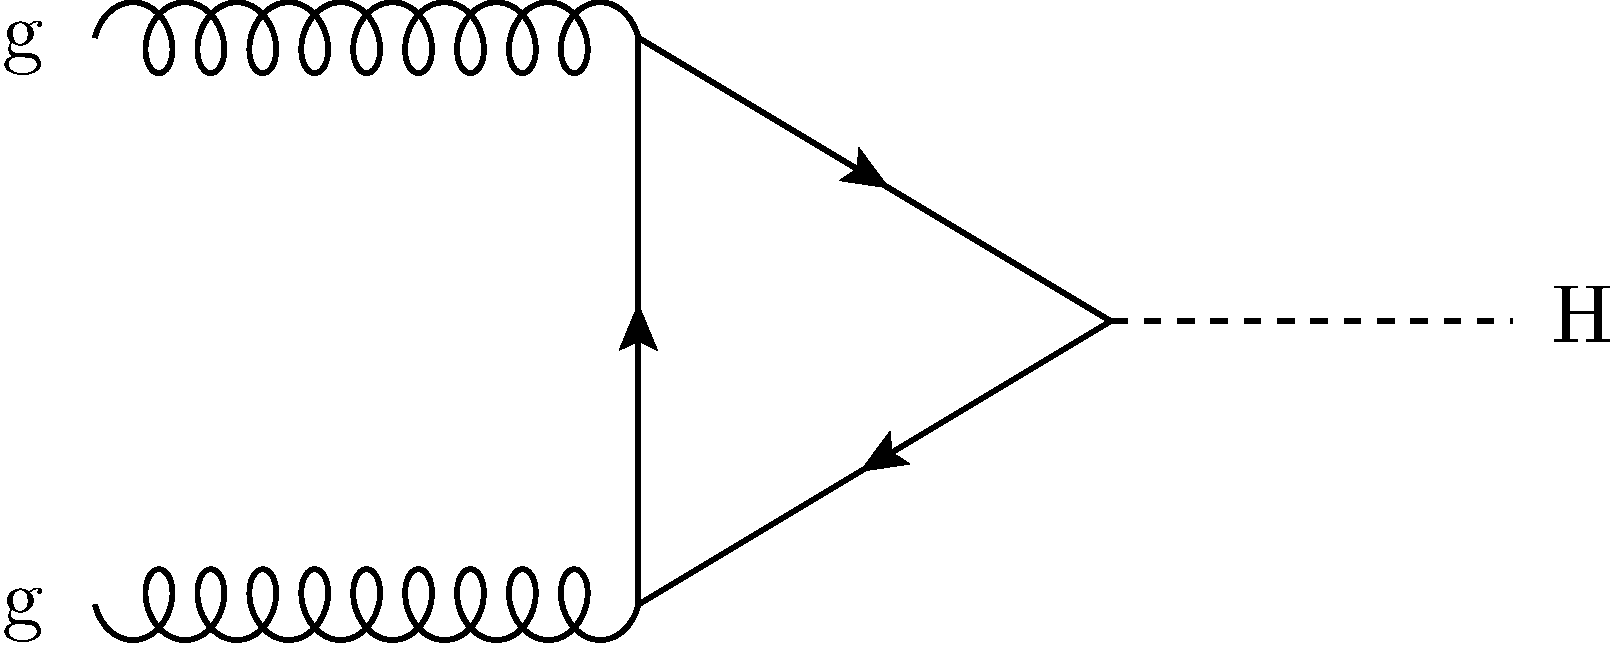
\includegraphics[width=0.48\textwidth]{plots/theory/feynman_ggH.pdf}}
\subfloat[]{
   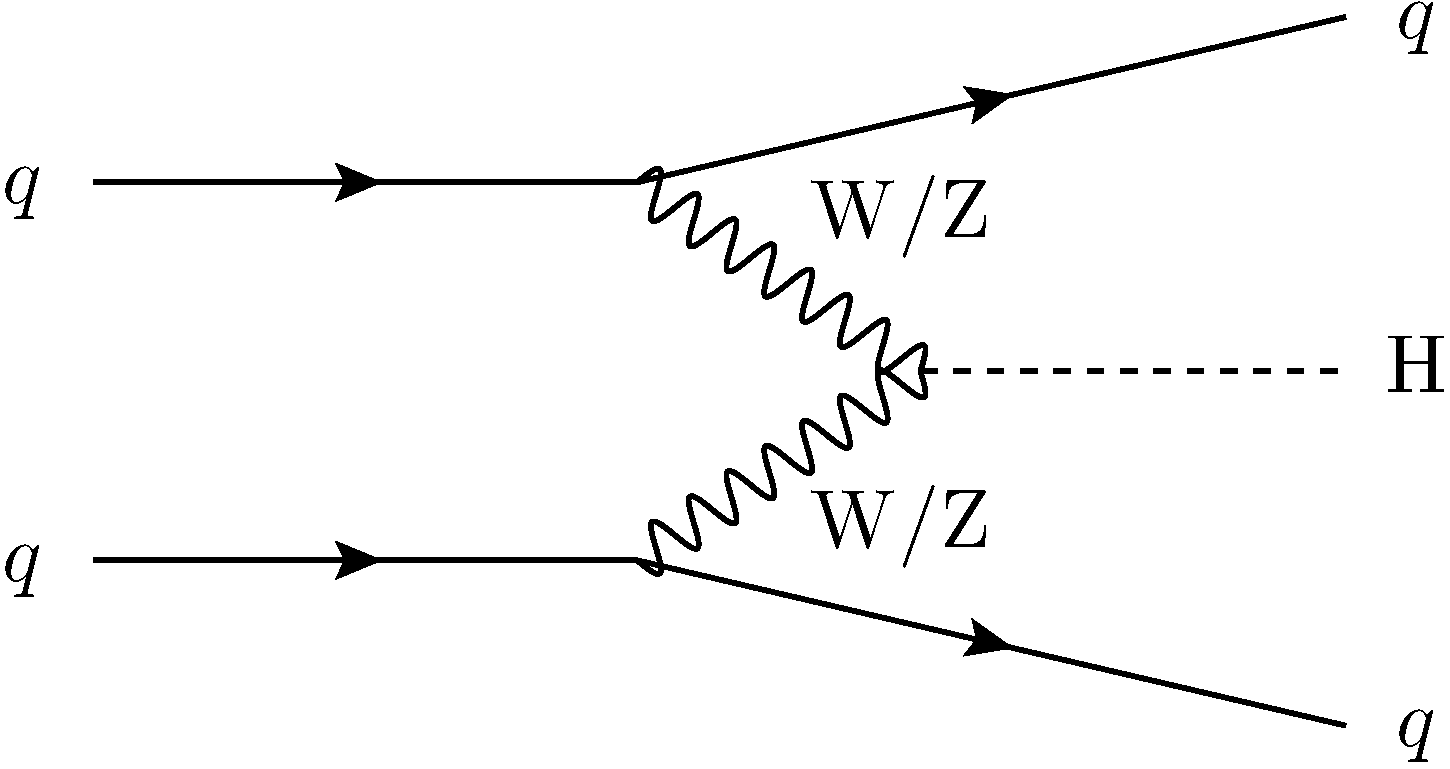
\includegraphics[width=0.4\textwidth]{plots/theory/feynman_qqH.pdf}}

\subfloat[]{
   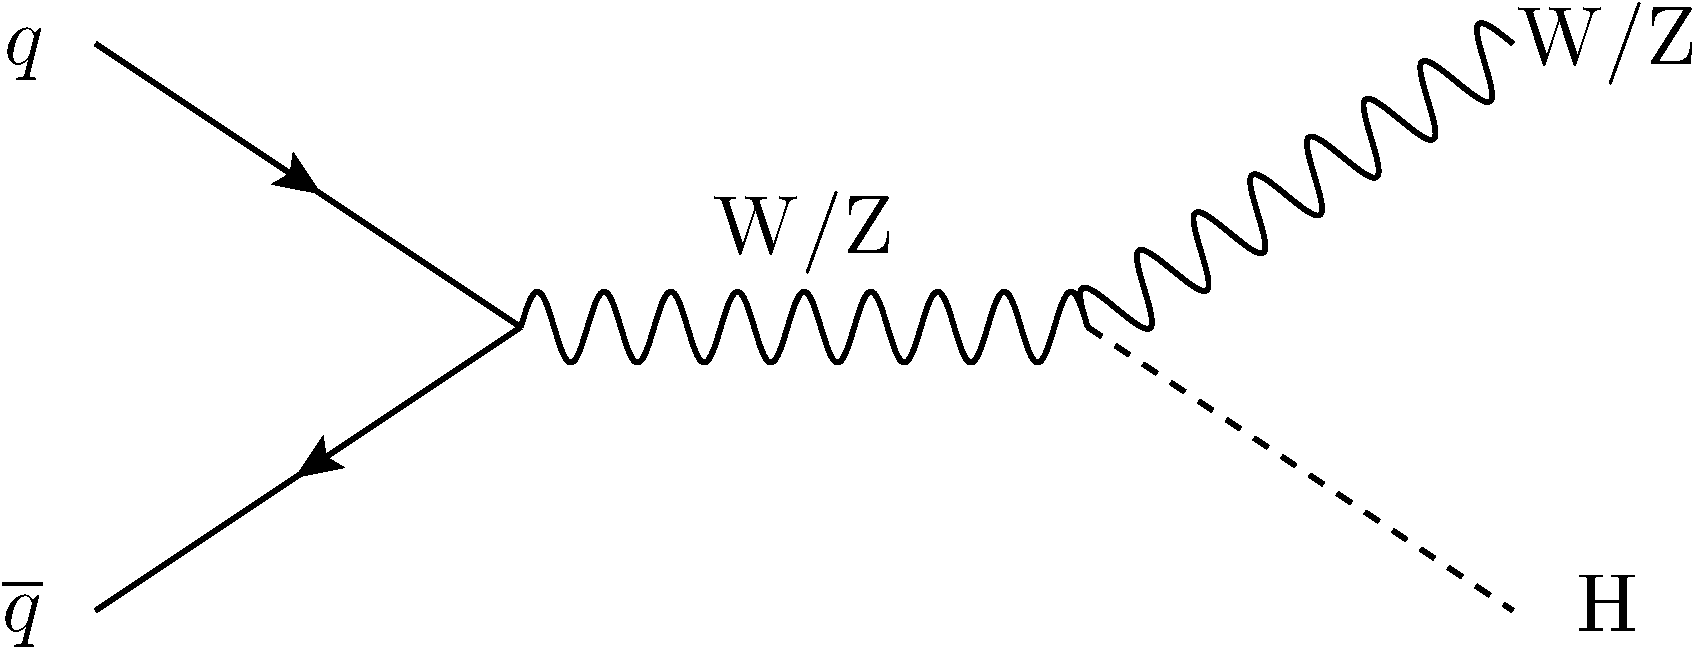
\includegraphics[width=0.48\textwidth]{plots/theory/feynman_VH.pdf}}
\subfloat[]{
   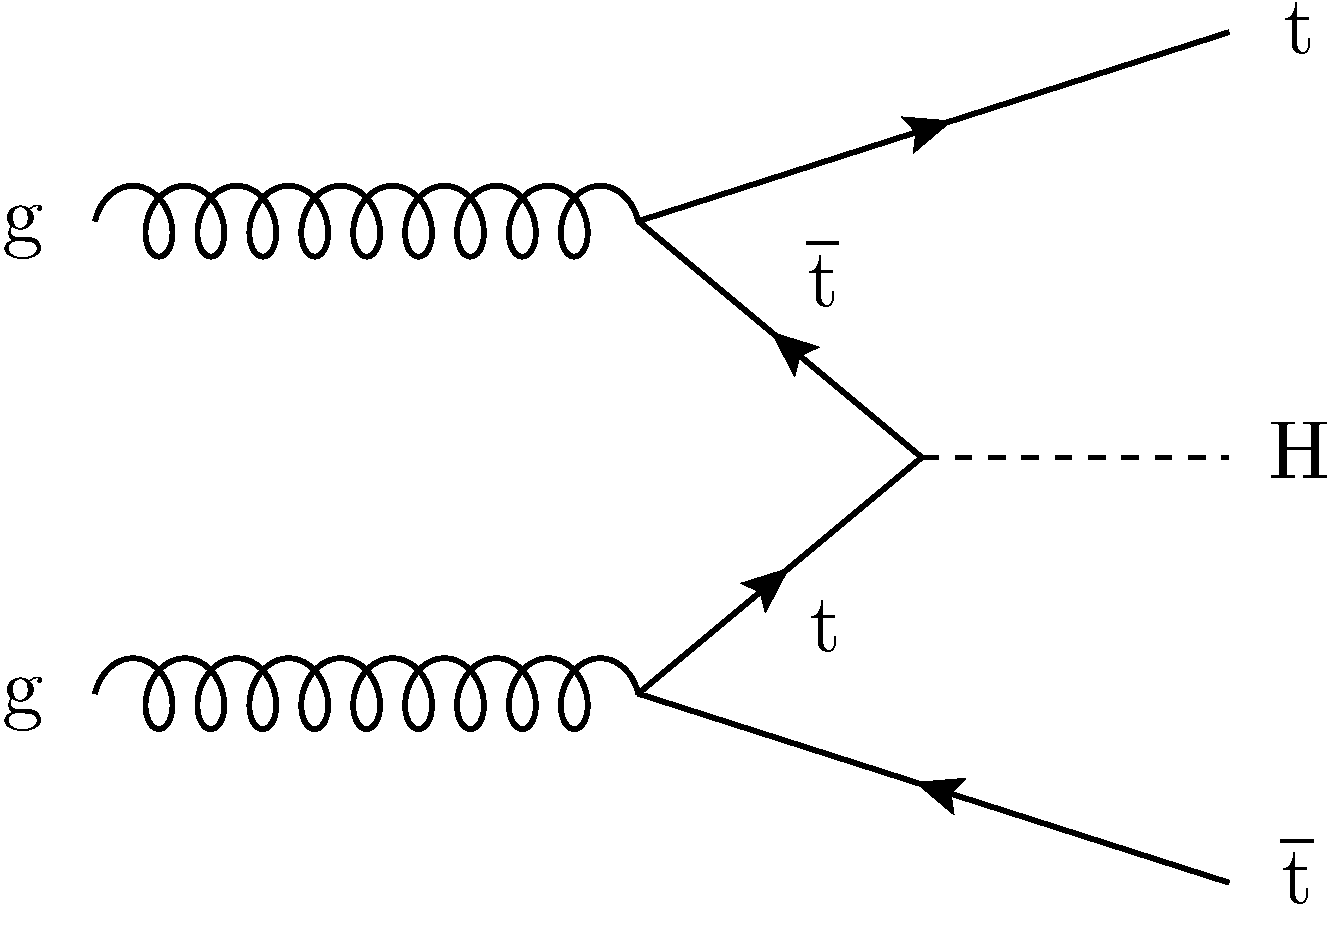
\includegraphics[width=0.4\textwidth]{plots/theory/feynman_ttH.pdf}}
\caption[Feynman diagrams for the dominant production processes of the SM Higgs
boson.]{Feynman diagrams for the dominant production processes of the SM Higgs
boson. Shown is a) gluon fusion, b) vector boson fusion and
associated production with c) vector bosons and d) top quarks.}
\label{fig:SMFeynmanDiagrams}
\end{figure}

Previous searches for the Higgs boson were carried out at LEP and the
Tevatron. LEP collided electrons and positrons at centre of mass
energies ($\sqrt{s}$) between $90$ and $209\,\GeV$. In such collisions the Higgs
boson is predominantly produced in association with a $\PZ$ boson, a process
referred to as ``Higgsstrahlung''. The decay channels used were predominantly decays
to $\Pqb\Paqb$ and $\Pgtp\Pgtm$ pairs. The fact that the Higgs boson was not
observed at LEP yields the exclusion of masses with $m_{\PH}<114.4\,\GeV$ at the
95\% \ac{CL} \cite{Barate:2003sz}. Searches were also performed by the CDF and D0 Collaborations at
the Tevatron accelerator, which collided protons and antiprotons with
$\sqrt{s}=1.96\,\TeV$. The searches were performed in a mass range of
$90$--$200\,\GeV$ and focussed on decays into $\Pqb\Paqb$, $\PWp\PWm$,
$\gamma\gamma$ and $\Pgtp\Pgtm$ pairs, with  $\Pqb\Paqb$ and $\PWp\PWm$ offering
the highest sensitivity. The combined results from the Tevatron yielded
exclusions of $m_{\PH}$ in the ranges $90$--$109\,\GeV$ and $140$--$184\,\GeV$
\cite{Aaltonen:2013kxa}. The results of such direct searches
can be combined with precision measurements of electroweak observables at LEP
and by the SLAC Large Detector (SLD) to constrain the mass of the Higgs
boson to $94^{+29}_{-24}\,\GeV$ \cite{lepewwg}, 
where the uncertainty incorporates experimental effects only.

The LHC provides a higher centre of mass energy than the Tevatron, and so
gives access to higher cross-sections and a wider range of Higgs masses. Figure
\ref{fig:SMHiggsXS} indicates the cross-sections of the different production
processes, for proton-proton collisions at $\sqrt{s}=8\,\TeV$ as used during the 
2012 operating period of the LHC. The gluon fusion production process dominates 
over the others by at least one order of magnitude in cross-section. 
Despite this, the other production modes are useful as they have specific 
topologies which can be exploited in the selection of signal-like events. 
The \ac{VBF} process is characterised by the two outgoing quarks which
hadronise to form jets with high momentum, typically found in the forward
detector region. Production via the associated production process consists of a vector
boson or a pair of top quarks in the final state, yielding multi-lepton and 
multi-jet final states with reduced backgrounds from other \ac{SM} processes.

\begin{figure}[htbp]
   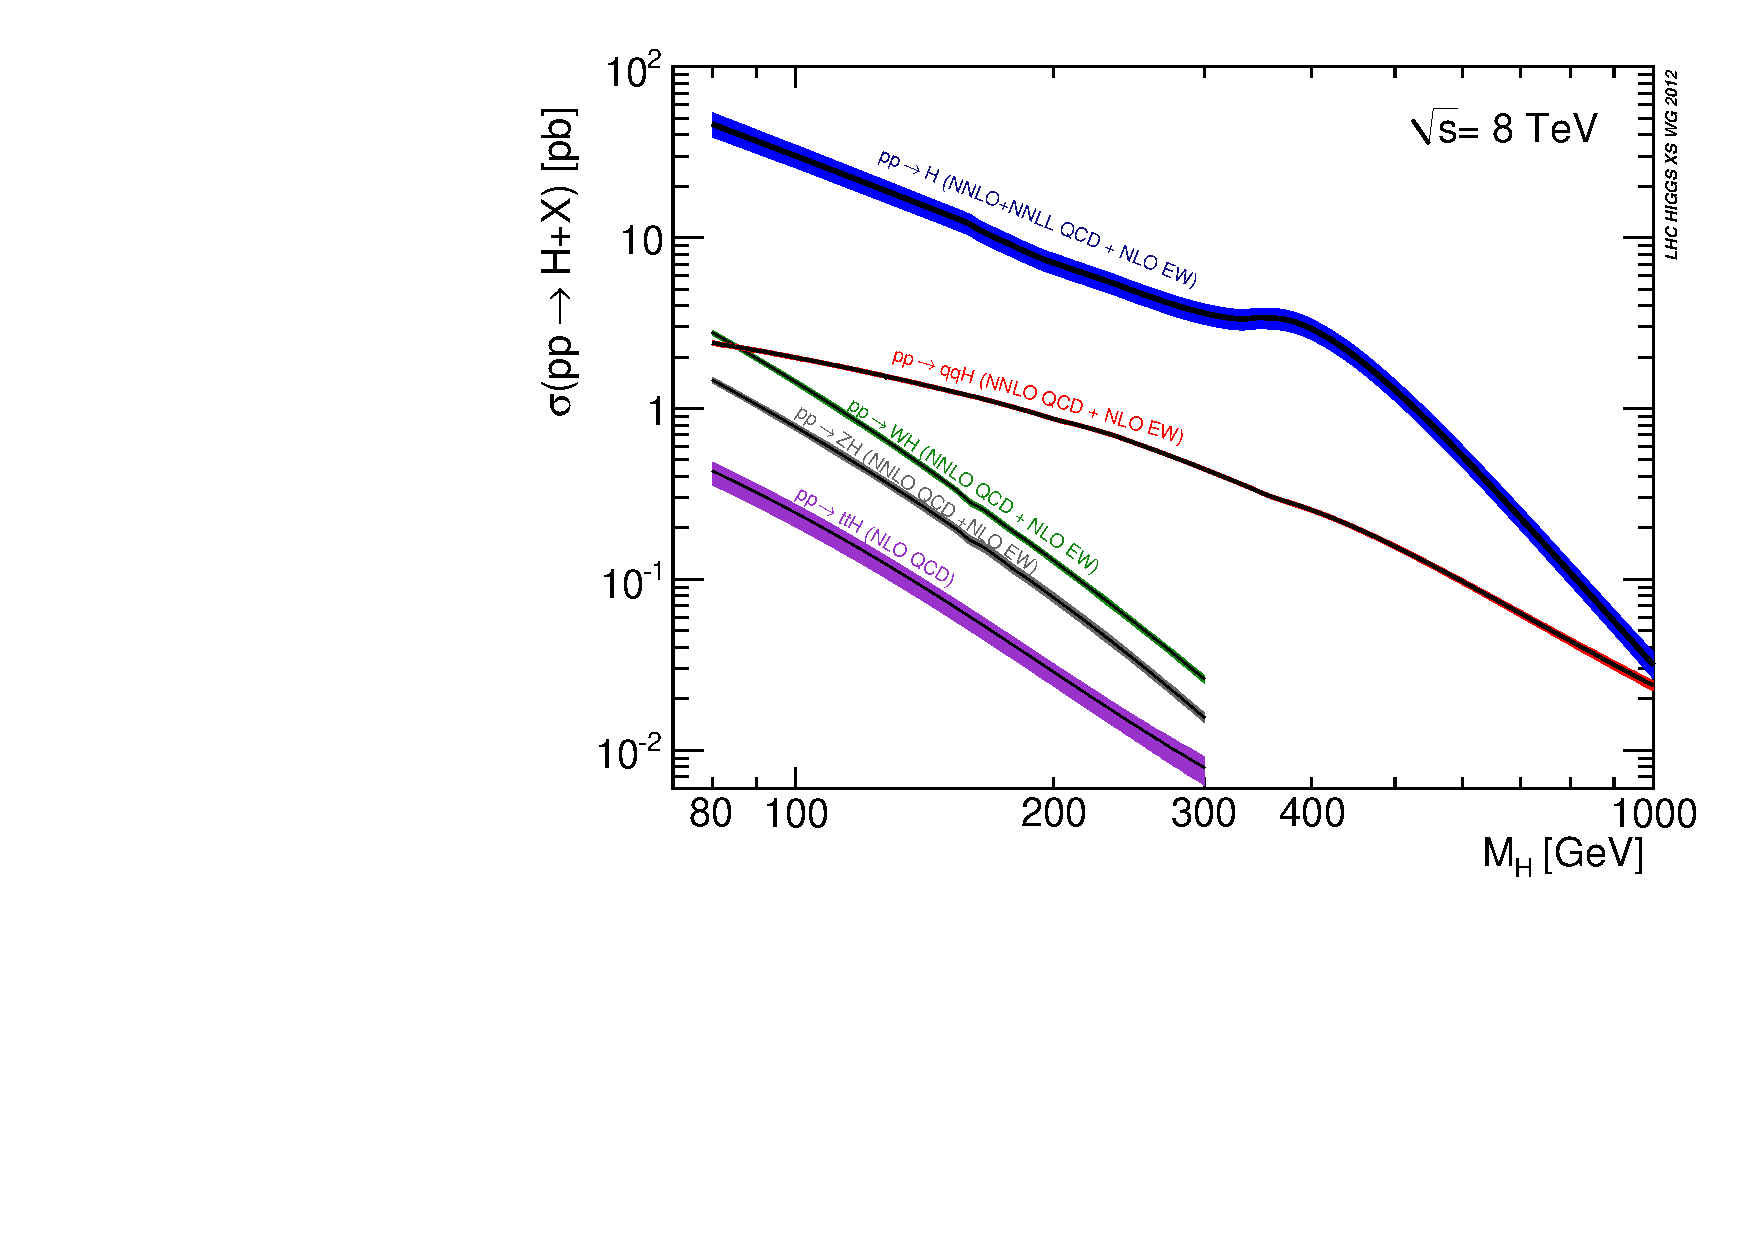
\includegraphics[width=0.7\textwidth]{plots/theory/Higgs_XS_8TeV_lx.pdf}
\caption[Cross sections for Higgs production processes at $\sqrt{s}=8\,\TeV$ for
a range of Higgs boson masses.]{Cross sections for Higgs production processes at
$\sqrt{s}=8\,\TeV$ for a range of Higgs boson masses $m_{\PH}$~\cite{Heinemeyer:2013tqa}. Across the
mass range the gluon-fusion mode dominates, followed by the vector boson fusion
and associated production modes. The widths of the lines represent the
theoretical uncertainties on the cross-section calculation.}
\label{fig:SMHiggsXS}
\end{figure}

The branching fractions to the different decay channels are shown in
figure~\ref{fig:SMHiggsBRs} for a range of possible Higgs masses. At low Higgs
boson masses, a variety of different decay channels are accessible. The decay
into two photons occurs via a fermion and $\PW$ loop, and decays to $\PWp\PWm$, $\PZ\PZ$,
$\Pqb\Paqb$ and $\Pgtp\Pgtm$ pairs are also possible. At higher Higgs masses
above $130\,\GeV$, the decays into $\PWp\PWm$, $\PZ\PZ$ are more kinematically
favourable and hence dominate. In the discovery of a Higgs boson, identication of
any of these decay channels is important, but the most sensitive channels for
discovery in the low mass region are $\Pphoton\Pphoton$ and $\PZ\PZ$ due to
their clean signatures. However, upon discovery of a Higgs boson, decays into 
fermions are particularly important
to establish the Yukawa couplings. In fermionic decays, the decay into
$\Pqb\Paqb$ dominates with a branching fraction of $\sim 80\%$ in this mass
range. However, this final state is difficult to disentangle from the large QCD
jet background at the LHC, meaning that the $\Pgtp\Pgtm$ final state has higher sensitivity.

\begin{figure}[htbp]
   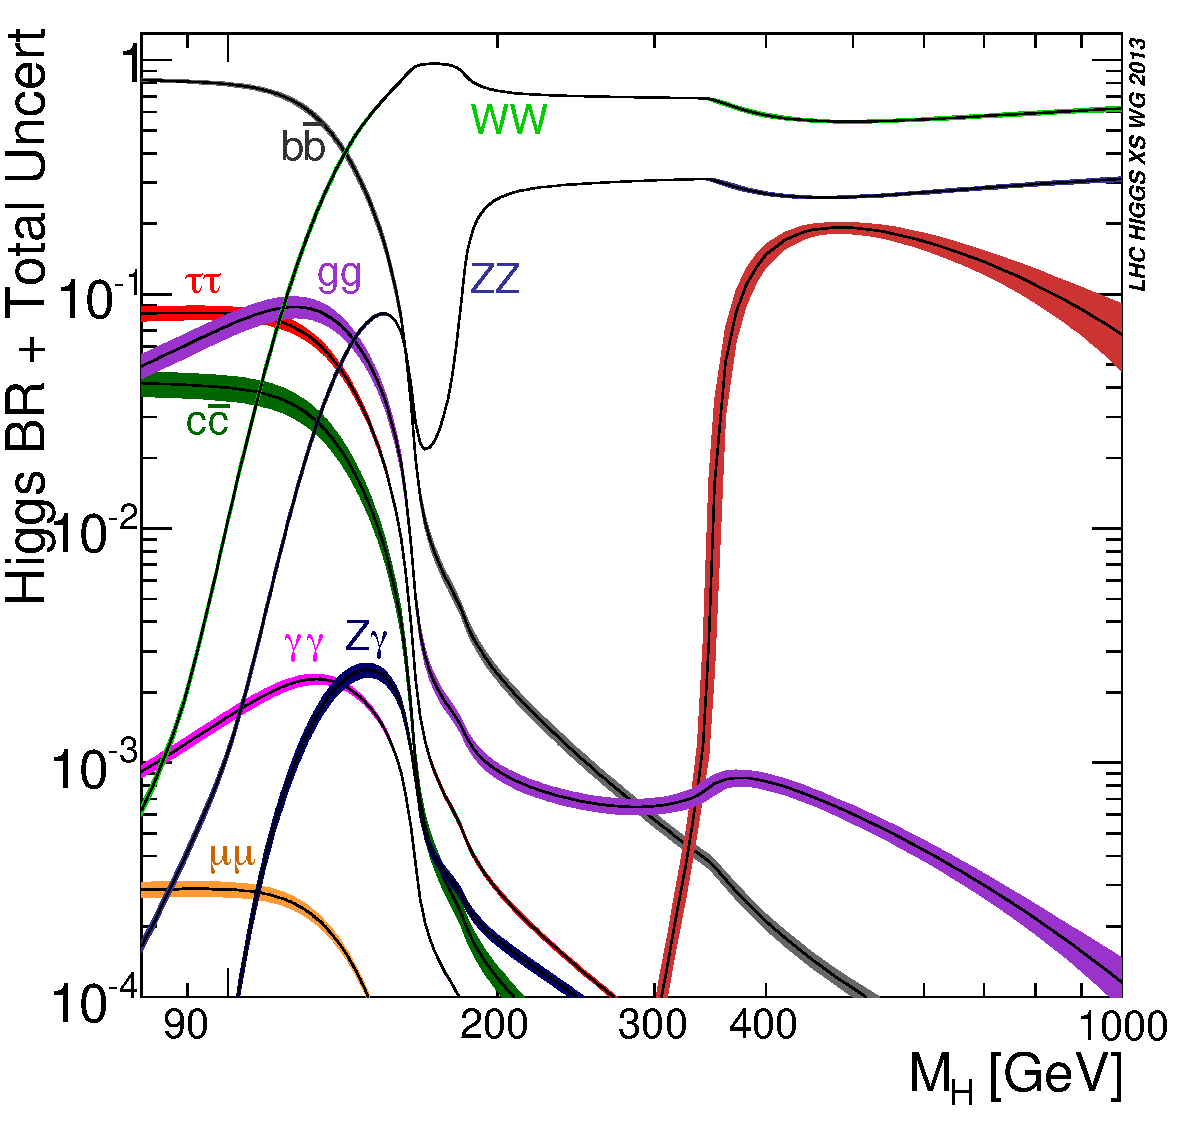
\includegraphics[width=0.6\textwidth]{plots/theory/Higgs_BR.pdf}
\caption[Higgs boson branching ratios in the SM for a range of Higgs boson
masses.]{Higgs boson branching ratios in the SM for a range of Higgs boson
masses $m_{\PH}$ \cite{Heinemeyer:2013tqa}. Whilst the $\PW\PW$ and $\PZ\PZ$
decay modes dominate at higher Higgs masses, at lower masses a wide range of
different final states is possible. The widths of the lines represent the
theoretical uncertainties on the branching ratio calculation.}
\label{fig:SMHiggsBRs}
\end{figure}

On 4 July 2012 the ATLAS and CMS Collaborations announced the discovery of a new
boson with a mass around $125\,\GeV$~\cite{CMSobservation125,ATLASobservation125}. 
Both experiments analysed approximately $5\,\invfb$ of data collected at 
$\sqrt{s}=7\,\TeV$ and $5$--$6\,\invfb$ at $\sqrt{s}=8\,\TeV$. The discovery was
made predominantly using the $\PZ\PZ$ and $\Pphoton\Pphoton$ decay modes with a
combined excess of events in data yielding a $5\sigma$ deviation from the
background-only expectation.

Run 1 of the LHC was completed in early 2013, increasing the dataset to
$\approx20\,\invfb$ at $8\,\TeV$. The increased dataset allows access to the less
sensitive decay modes. The most recent combination of CMS Higgs results yields a
best fit mass of
$125.02^{+0.26}_{-0.27}(\text{stat})^{+0.14}_{-0.15}(\text{syst})\,\GeV$ and a
signal strength relative to the \ac{SM} expectation of
$1.00\pm0.09(\text{stat})^{+0.08}_{-0.07}(\text{theo})\pm0.01(\text{syst})$,
combining results from the $\Pphoton\Pphoton$, $\PWp\PWm$, $\PZ\PZ$,
$\Pqb\Paqb$, $\Pgtp\Pgtm$ and $\APmuon\Pmuon$ final states, as well as 
searches for the $\Pqt\Pqt\PH$ production mode and searches for an invisible
Higgs \cite{CMScomb}. Within the combination is a study of the compatibility of
the couplings in each decay mode with the \ac{SM}. 
These channels all show consistency with the \ac{SM}
predictions for a $125\,\GeV$ Higgs boson. Other analyses from ATLAS have
studied the production rates and couplings in various channels~\cite{Aad:2014eva,Aad:2014lwa,Aad:2015vsa}, 
and results from both ATLAS and CMS study the spin-parity quantum
numbers~\cite{Chatrchyan:2013mxa,Chatrchyan:2013iaa,Aad:2013xqa} and limits on
the decay width~\cite{Khachatryan:2014iha} and invisible branching
fraction~\cite{Aad:2014iia,Chatrchyan:2014tja}. No significant deviations from \ac{SM}
predictions have been found to date in any of these results.

Future studies will further test the compatibility of the observed boson with
the \ac{SM} Higgs, including discovery and precision measurements in the
channels which are less sensitive and require more data. 
The most recent CMS results for the search for the Higgs boson in the $\HToTauTau$
decay channel, corresponding to the complete Run 1 dataset and as included in
the most recent combination, are reported in chapter~\ref{chap:htt-sm}.

\section{Higgs boson physics beyond the standard model}
\label{sec:BSM}

\subsection{Motivation for theories beyond the standard model}
\label{sec:hierarchyproblem}

Despite its successes, the \ac{SM} is known to have some shortcomings. As a
theory, it does not predict a candidate to account for the large fraction of
non-radiating, non-baryonic dark matter in the universe. It also does not
predict the non-zero neutrino masses which are inferred from experimental
results in neutrino oscillations~\cite{PDG}. As a theory it also suffers from a
shortcoming in that the weak and strong coupling constants associated with the
$SU(3)_{C} \times SU(2)_{L} \times U(1)_{Y}$ gauge group do not intersect at a
high energy scale, as would be hoped for in a unified theory~\cite{Amaldi:1991cn}. It also does not
incorporate gravity. Finally, one shortcoming is of particular relevance 
in the Higgs sector, and is known as the Hierarchy Problem.

It is generally accepted that the \ac{SM} is an effective theory up to some
energy scale $\Lambda$ where the effect of new physics becomes important. 
The Higgs mass at tree level is given by $\sqrt{2}\mu_{SM}$. Radiative
corrections adjust the mass as:
\begin{equation}
m_{\PH_{SM}}^{2} = 2\mu_{SM}^{2} - \Delta m_{\PH}^{2}. 
\end{equation}
It can be shown that the size of the correction, $\Delta m_{\PH}^{2}$, is
quadratically dependent on $\Lambda$~\cite{Carena:2002es}:
\begin{equation}
\Delta m_{\PH}^{2} \sim \mathcal{O}(\Lambda^{2}).
\end{equation}
The scale $\Lambda$ can be as high as the Planck scale, where gravitational
interactions become significant~\cite{Griffiths:2008nx}. For a $\Lambda$ at the Planck scale then
$\Delta m_{\PH}^{2}$ is some 30 orders of magnitude larger than 
$m_{\PH_{SM}}^{2}$ for $m_{\PH_{SM}}<1\,\TeV$. This means that the bare Higgs
boson mass requires extreme fine tuning of the bare mass term $2\mu_{SM}^{2}$ to
allow cancellation. Figure~\ref{fig:HiggsMassLoops} indicates the radiative
corrections to the Higgs mass resulting from a fermion and a boson loop.

\begin{figure}[htbp]
\subfloat[]{
   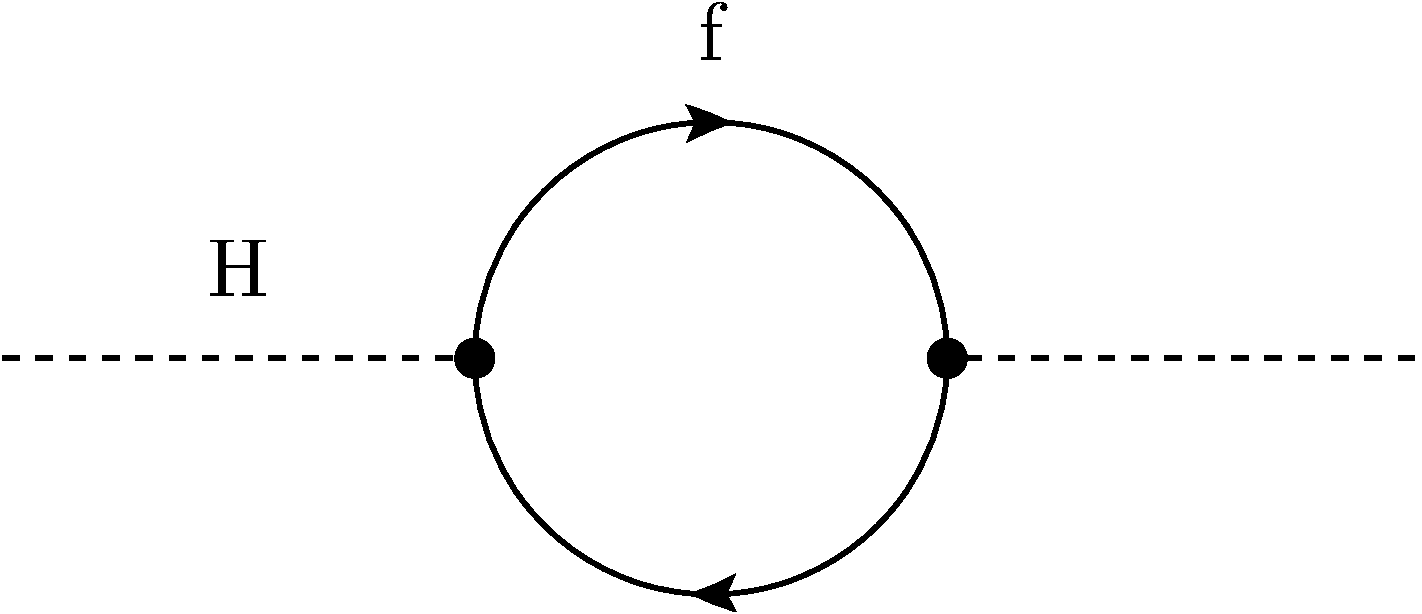
\includegraphics[width=0.48\textwidth]{plots/theory/HiggsMass_fermionLoop.pdf}}
\subfloat[]{
   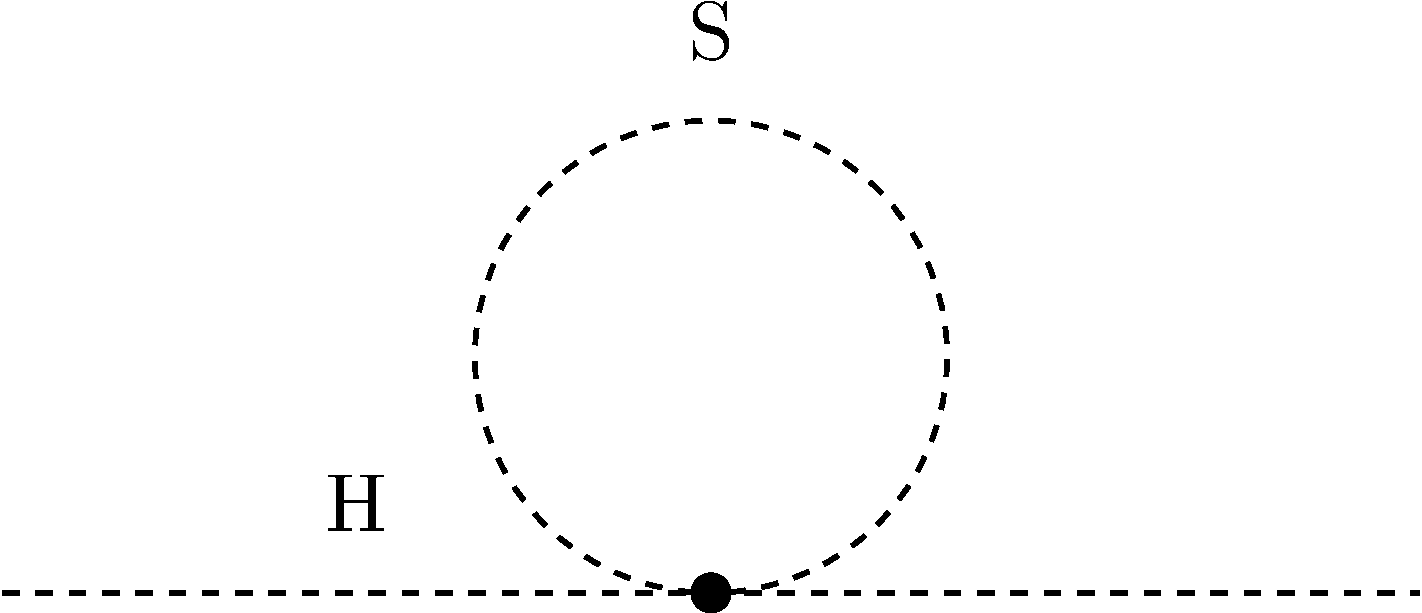
\includegraphics[width=0.48\textwidth]{plots/theory/HiggsMass_bosonLoop.pdf}}
\caption{Feynman diagrams illustrating the one-loop radiative corrections to the Higgs
mass for a fermion, $f$ (a) and scalar boson, $S$ (b)}
\label{fig:HiggsMassLoops}
\end{figure}

Many \ac{BSM} theories are proposed which provide solutions to this Hierarchy
problem. One of the most popular is \ac{SUSY}. In \ac{SUSY}, a new
symmetry between fermions and bosons is introduced~\cite{Martin:1997ns}. This
can be used to solve the issue with the Higgs mass correction by exploiting the
fact that the bosonic and fermionic loop contributions illustrated in 
figure~\ref{fig:HiggsMassLoops} contribute with opposite signs. Thus the symmetry
between bosons and fermions permits the cancellation of $\Delta m_{\PH}^{2}$
terms. In SUSY models, each \ac{SM} fermion has a boson superpartner and each
\ac{SM} boson has a fermion superpartner. If \ac{SUSY} is an unbroken symmetry then
the superpartners have exactly the same mass as their \ac{SM} partner. Since
none of these superpartner particles have been observed in nature, \ac{SUSY} must be
a broken symmetry in which the superpartner masses are larger than the
\ac{SM} masses. The necessity to avoid further fine tuning means the scale of
\ac{SUSY} cannot be much larger than $\mathcal{O}(1\,\TeV)$. An additional motivation
for \ac{SUSY} is the fact that the lightest \ac{SUSY} particles, if stable, could provide
candidates for dark matter. Also the behaviour of the running coupling
constants is modified such that all three intersect at
$\mathcal{O}(10^{16}\,\GeV)$~\cite{Amaldi:1991cn}.

\subsection{The Higgs sector in the MSSM}
\label{sec:mssmhiggs}

The simplest addition of \ac{SUSY} to the \ac{SM} results in the \ac{MSSM}. The
\ac{MSSM} is an extension to the \ac{SM} which minimises the numbers of
additional fields and interactions while preserving R-parity~\cite{Dimopoulos:1981zb}. R-parity
is an operator with eigenvalues of 1 for \ac{SM} particles and -1 for
superparners. It is required to be conserved in order to explain the stability
of the proton~\cite{}. In order to generate the appropriate mass terms for the up-type 
and down-type fermions, two complex scalar weak isospin doublet fields
$\phi_{\Pqu}$ and $\phi_{\Pqd}$ are added:
\begin{equation}
\phi_{\Pqu} = \begin{pmatrix}\phi_{\Pqu}^{+} \\ \phi_{\Pqu}^{0} \end{pmatrix}, \quad
\phi_{\Pqd} = \begin{pmatrix}\phi_{\Pqd}^{0} \\ \phi_{\Pqd}^{-} \end{pmatrix}. 
\end{equation}
This results in an \ac{MSSM} Lagrangian with potential terms as:
\begin{equation}
V=\mu(\phi_{\Pqu}^{+}\phi_{\Pqd}^{-} - \phi_{\Pqu}^{0}\phi_{\Pqd}^{0}),
\end{equation}
where $\mu$ is the \ac{MSSM} equivalent of the \ac{SM} Higgs mass parameter
$\mu_{SM}$. This potential provides spontaneous symmetry breaking as in the
\ac{SM} case yielding VEVs parameterised by:
\begin{equation}
\bra{0}\phi_{\Pqu}\ket{0} = \begin{pmatrix} 0 \\ v_{\Pqu}  \end{pmatrix}, \quad
\bra{0}\phi_{\Pqd}\ket{0} = \begin{pmatrix} v_{\Pqd} \\ 0 \end{pmatrix},
\end{equation}
which are related to the \ac{SM} value and hence $m_{\PW}$ by: 
\begin{equation}
v^{2} = v_{\Pqu}^{2} +  v_{\Pqd}^{2} =  \frac{2m_{\PW}^{2}}{g},
\end{equation}
Thus in the \ac{MSSM}, the
phenomenology is conveniently described in terms of the ratio of the VEVs,
$\tan\beta = v_{u}/v_{d}$, which is not directly predicted by the model.
Of the eight initial degrees of freedom, three become longitudinal states of the
$\PW^{\pm}$ and $\PZ$ bosons which leaves five massive Higgs fields. These
result in five physical Higgs bosons; a neutral pseudoscalar $\PA$, two neutral
scalars $\Ph,\PH$ and two charged scalars $\PH^{\pm}$. These bosons are defined
by the mixing of $\phi_{\Pqu}$ and $\phi_{\Pqd}$, parameterised by a mixing
angle $\alpha$ in addition to $\beta$:
%Check this - typo in Mike's thesis?
\begin{equation}
\PA = \sqrt{2}(\text{Im}(\phi_{\Pqu}^{0})\cos\beta +
\text{Im}(\phi_{\Pqd}^{0})\sin\beta), \\ 
\begin{pmatrix} h \\ H \end{pmatrix} = \sqrt{2} 
\begin{pmatrix} \cos\alpha & -\sin\alpha \\ \sin\alpha & \cos\alpha \end{pmatrix}
\begin{pmatrix} \text{Re}(\phi_{\Pqu}^{0}) - v_{\Pqu} \\ \text{Re}(\phi_{\Pqd}^{0}) -
v_{\Pqd}\end{pmatrix}, \\
\PH^{+} = \phi_{\Pqu}^{+} \cos \beta + \phi_{\Pqd}^{-\dagger} \sin \beta,\\
\PH^{-} = \phi_{\Pqu}^{+\dagger} \cos \beta + \phi_{\Pqd}^{-} \sin \beta.
\end{equation}
The self interactions of the scalar fields are not independent parameters in the
\ac{MSSM} and can be expressed in terms of $g$ and $g'$. As a result, the masses
and couplings of the \ac{MSSM} Higgs bosons can be determined at tree level by
two free parameters: $\tan\beta$ and the mass of one of the Higgs bosons,
conventionally chosen to be the mass of the pseudoscalar, $m_{\PA}$. The masses
of the other Higgs bosons can then be expressed as:
\begin{equation}
m_{\Ph}^{2} = \frac{1}{2} \left( m_{\PA}^{2} + m_{\PZ}^{2} - \sqrt{(m_{\PA}^{2} +
m_{\PZ}^{2})^{2} - 4m_{\PZ}^{2}m_{\PA}^{2}\cos{2\beta}^{2} }\right) ,
\label{eq:mh}\\
m_{\PH}^{2} = \frac{1}{2} \left( m_{\PA}^{2} + m_{\PZ}^{2} + \sqrt{(m_{\PA}^{2} +
m_{\PZ}^{2})^{2} - 4m_{\PZ}^{2}m_{\PA}^{2}\cos{2\beta}^{2} }\right) , \\
m_{\PH^{\pm}} = m_{\PA}^{2} + m_{\PW}^{2},
\end{equation}
where $m_{\Ph}$, $m_{\PH}$ and $m_{\PH^{\pm}}$ are the masses of the $\Ph$,
$\PH$ and $\PH^{\pm}$ bosons respectively. This yields a constraint on $\alpha$:
\begin{equation}
\cos^{2}(\beta-\alpha) = \frac{m_{\Ph}^{2}(m_{\PZ}^{2} -
m_{\Ph}^{2})}{m_{\PA}^{2}(m_{\PH}^{2} - m_{\Ph}^{2}) }.
\end{equation}
Equation \ref{eq:mh} yields an upper bound on $m_{\Ph}$:
\begin{equation}
m_{\Ph} \leq m_{\PZ} |\cos{2\beta}|. 
\end{equation}

This means that at tree level, the mass of the lightest scalar Higgs cannot
exceed that of the $\PZ$ boson ($91.2\,\GeV$). However, the tree level masses and
couplings are modified by higher order corrections. The dominant effect is from
incomplete cancellation of the top and stop (the superpartner of the top) loops.
These corrections, as illustrated in figure \ref{fig:HiggsMassLoops}, do not
completely cancel in the case that \ac{SUSY} is broken. Hence the size of the
corrections is strongly dependent on the top and stop masses, where the stop
mass depends on $\mu$ and the parameters describing \ac{SUSY} breaking. The upper
bound of $m_{\Ph}$ is increased by these radiative corrections and is maximised
for large $m_{\PA}$ ($\gg m_{\PZ}$) and $\tan\beta$ ($\gg1$). The maximum value of
$m_{\Ph}$ for a particular choice of $m_{\PA}$ and $\tan\beta$ is denoted
$m_{\Ph}^{\text{max}}$. If the scale of SUSY breaking, $M_{\text{SUSY}}$, is
chosen to be $1\,\TeV$, $m_{\Ph}^{\text{max}} \approx 135\,\GeV$.

\subsection{Searching for a neutral MSSM Higgs boson}
\label{sec:LHCMSSMHiggs}

It is important that the phenomenology of Higgs bosons, including the higher
order corrections, is understood in order to define the masses of the neutral
Higgs bosons and hence optimise an experimental search for them. This is
complicated by the number of \ac{SUSY} breaking parameters in the \ac{MSSM}. Hence it
is conventional to study particular benchmark scenarios where the \ac{SUSY} breaking
parameters and $\mu$ are fixed to a choice of values and only $m_{\PA}$ and
$\tan\beta$ are varied~\cite{Carena:2002es}. One such scenario is the $m_{\Ph}^{\text{max}}$ scenario
in which $m_{\Ph}=m_{\Ph}^{\text{max}}$ for high $m_{\PA}$ and $\tan\beta$
values, using the choice $M_{\text{SUSY}} = 1\,\TeV$ and $\mu = \pm 200\,\GeV$.
Other alternative benchmark scenarios are discussed in 
section~\ref{sec:mssmbenchmarks}. 

Figure~\ref{fig:mhmaxmasses} indicates the
masses of each of the Higgs bosons in the $m_{h}^{\text{max}}$ scenario
for $\tan\beta=3$ and $\tan\beta=30$ as a function of the mass of the
pseudoscalar $m_{\PA}$. Two different regimes of the $m_{\Ph}^{\text{max}}$
scenario can be considered, in which one of the neutral scalars is approximately
degenerate in mass with the pseudoscalar and has similar couplings. 
At large $\tan\beta$ and for $m_{\PA} \ll m_{\Ph}^{\text{max}}$, $m_{\PA}
\approx m_{\Ph}$ and the couplings of the $\PA$ and $\Ph$ are very similar. The
couplings of the $\PA$ and $\Ph$ bosons to down-type fermions 
are enhanced by a factor $\sim \tan\beta$ relative to the \ac{SM} value, with
negligible couplings to vector bosons. The scalar $\PH$ has couplings
close to those in the \ac{SM}. In the limit where $m_{\PA} \gg
m_{\Ph}^{\text{max}}$, 
$m_{\PA} \approx m_{\PH}$ and the couplings of the $\PA$ and $\PH$ are
very similar. The couplings of the $\PA$ and $\PH$ bosons to down-type fermions 
are enhanced by a factor $\sim \tan\beta$ relative to the \ac{SM} value, 
with negligible couplings to vector bosons. The scalar $\Ph$ has couplings
close to those in the \ac{SM}. 

\begin{figure}[htbp]
   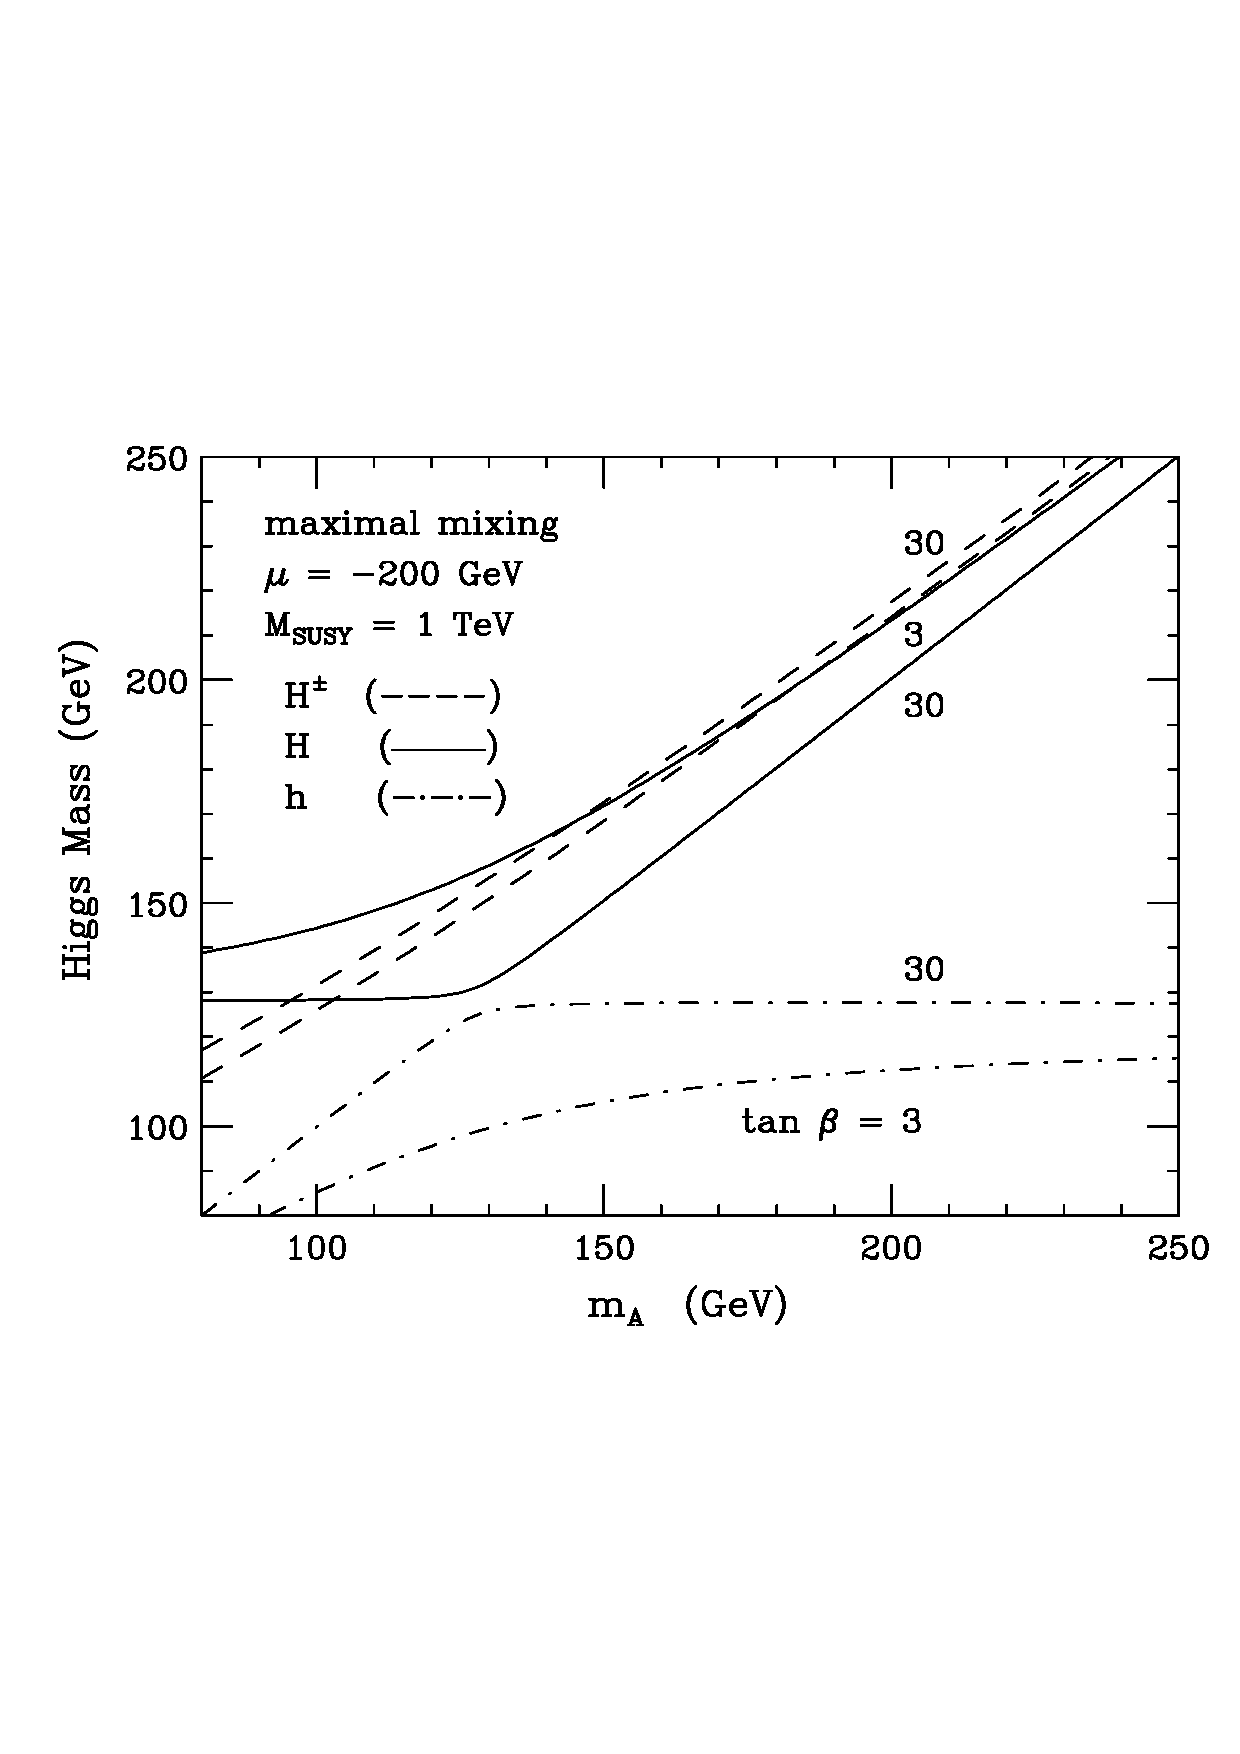
\includegraphics[width=0.7\textwidth]{plots/theory/mssm_masses_mhmax.pdf}
\caption[Masses of the $\Ph$, $\PH$ and $\PH^{\pm}$ bosons in the
$m_{\Ph}^{\text{max}}$ scenario as a function of $m_{\PA}$.]{Masses of the $\Ph$, $\PH$ and $\PH^{\pm}$ bosons in the
$m_{\Ph}^{\text{max}}$ scenario as a function of $m_{\PA}$. Values are shown for
$\tan\beta=3$ and $\tan\beta=30$ \cite{Carena:2002es}.}
\label{fig:mhmaxmasses}
\end{figure}

The effect of enhanced couplings to down-type fermions is illustrated by the
branching ratios of the $\PA$, shown in figure \ref{fig:mhmaxBRs} for $\tan\beta$
values of 10 and 50. It can be seen that the $\Pgt\Pgt$ decay mode has a large
branching ratio for a large range of $m_{\PA}$ and $\tan\beta$ points. This
motivates searches for the \ac{MSSM} Higgs bosons in the final state of $\Pgt\Pgt$. 
Chapter \ref{chap:htt-mssm} discusses the most recent results 
from direct searches for neutral \ac{MSSM} Higgs bosons using the $\Pgt\Pgt$
final state with the CMS detector.

\begin{figure}[htbp]
\subfloat[]{
   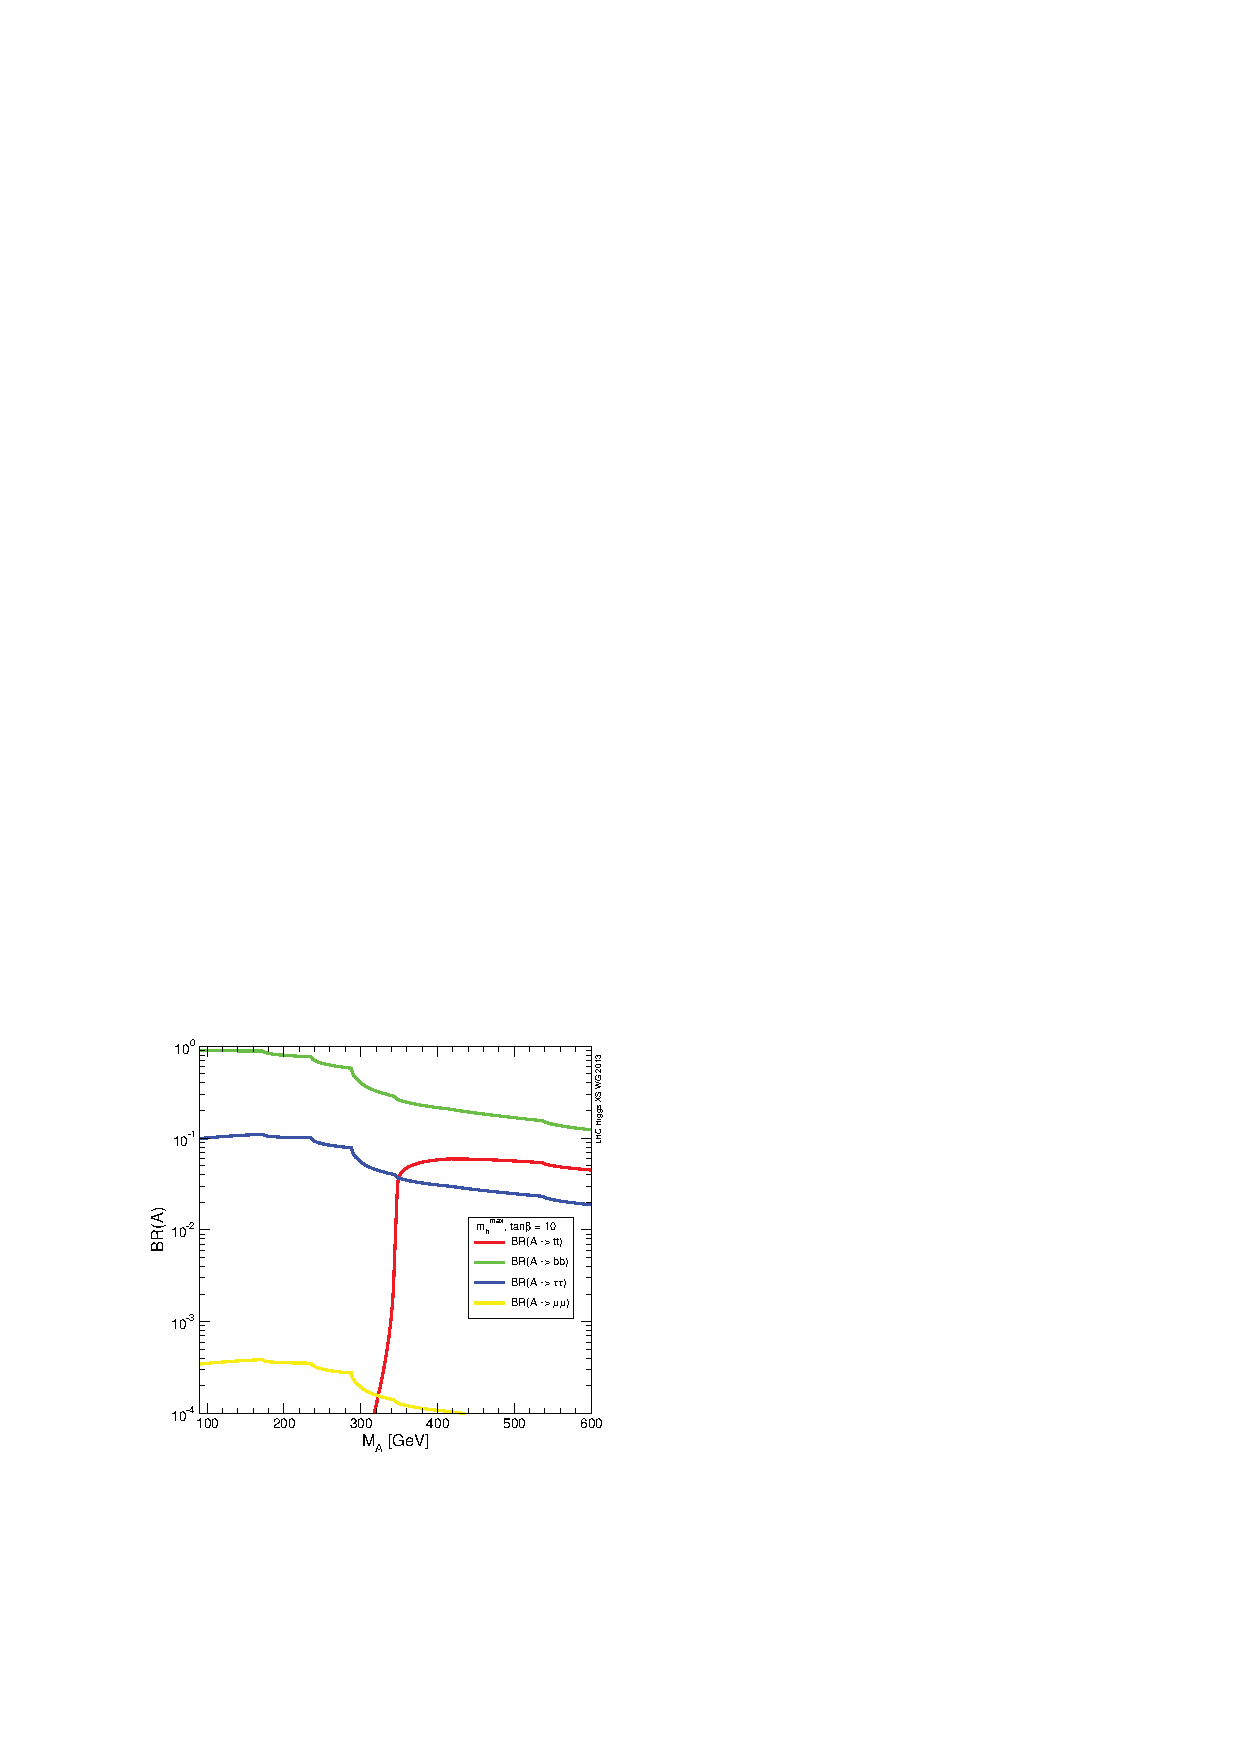
\includegraphics[width=0.5\textwidth]{plots/theory/BR_A_tanb10_mhmax.pdf}}
\subfloat[]{
   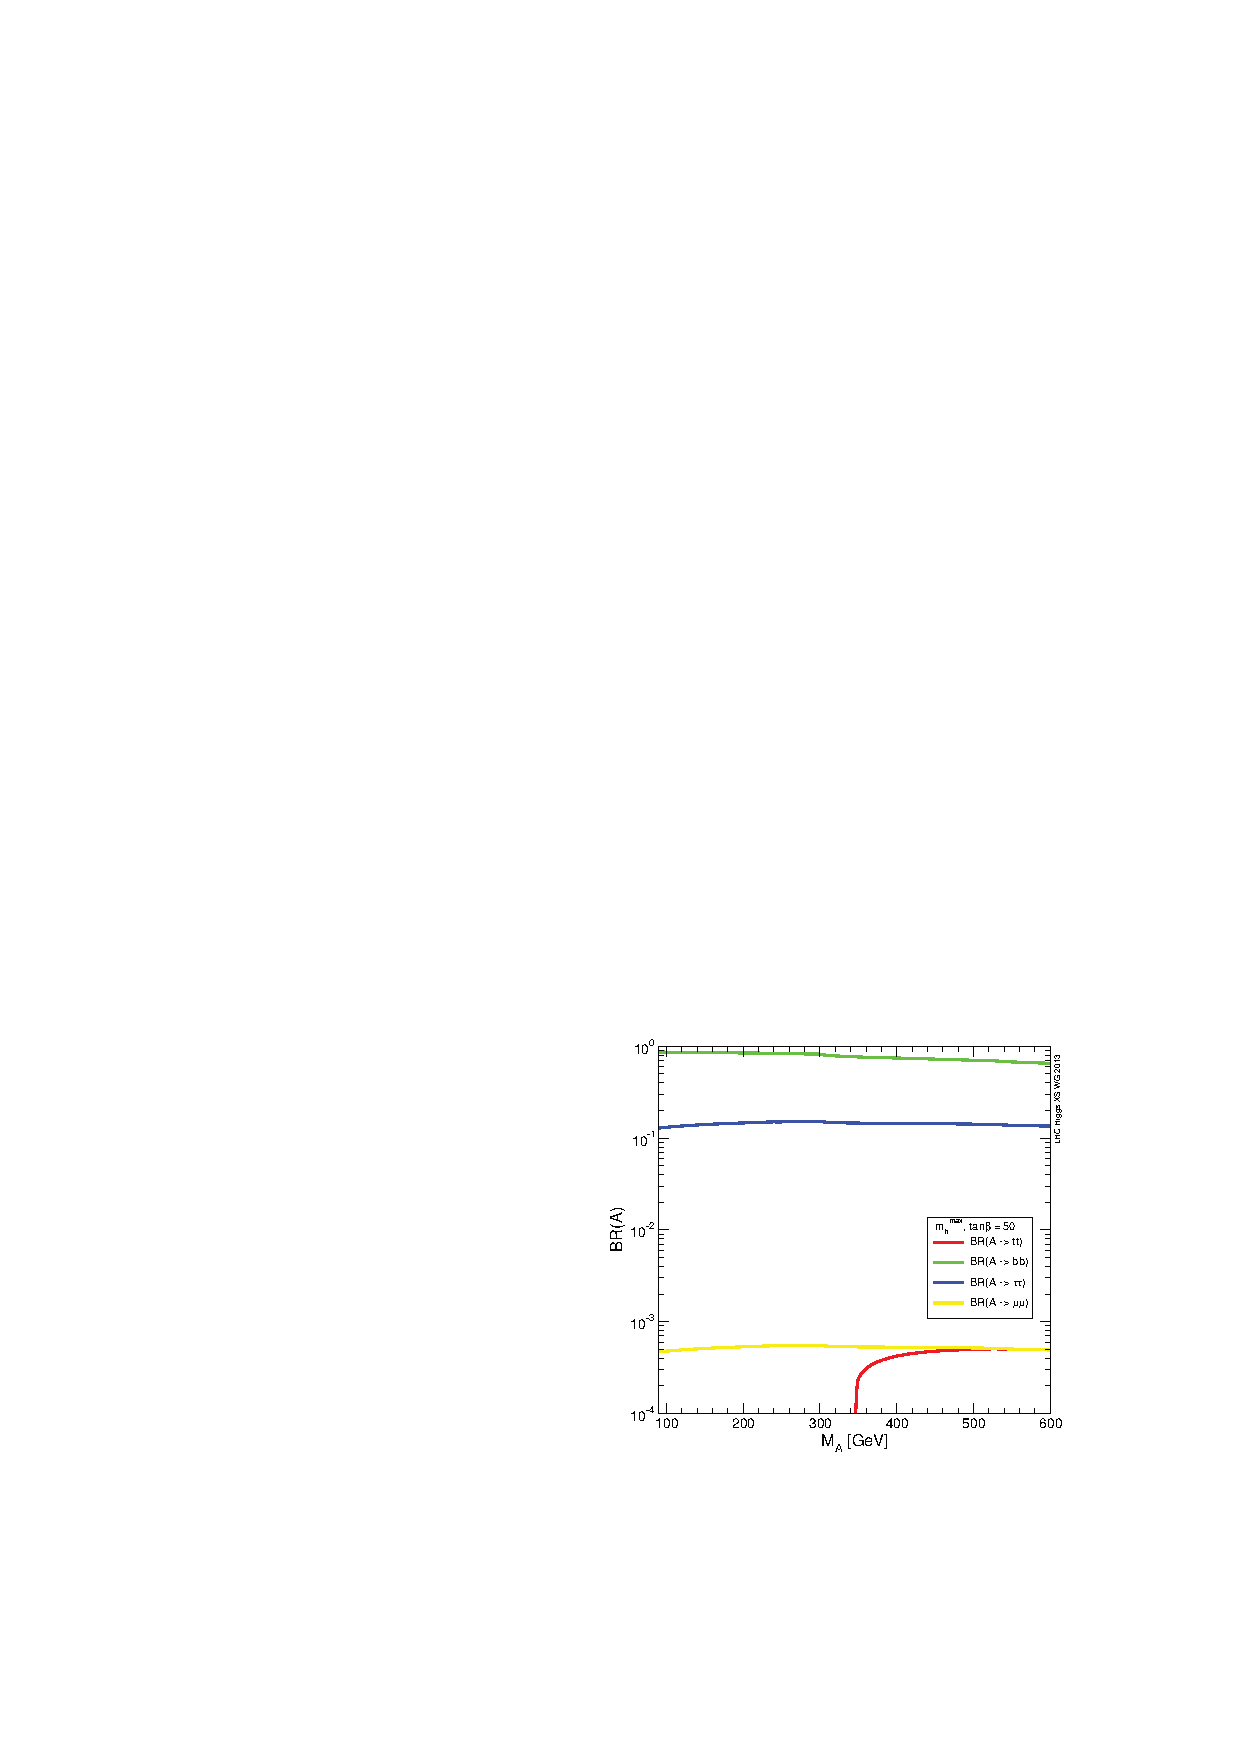
\includegraphics[width=0.5\textwidth]{plots/theory/BR_A_tanb50_mhmax.pdf}}
\caption[Branching ratios of the pseudoscalar Higgs boson $\PA$ in the
$m_{\Ph}^{\text{max}}$ scenario.]{Branching ratios of the pseudoscalar Higgs boson $\PA$ in the
$m_{\Ph}^{\text{max}}$ scenario for $\tan\beta=10$ (a) and $\tan\beta=50$
(b) \cite{Heinemeyer:2013tqa}.}
\label{fig:mhmaxBRs}
\end{figure}

Analogously to the \ac{SM} Higgs production, the dominant production mode at
small $\tan\beta$ is the gluon fusion process, denoted
$\Pgluon\Pgluon\to\Pphi$, where $\Pphi$ denotes any of the three neutral Higgs
bosons, $\Pphi=\PH,\PA,\Ph$. As in the \ac{SM} case the gluon fusion process
proceeds via a quark loop, which at low $\tan\beta$ is dominated by top quarks
but at high $\tan\beta$ the $\Pqb$-quark loops dominate due to enhanced couplings to
down-type fermions. At large $\tan\beta$, the dominant production mechanism is
Higgs radiation by $\Pqb$-quarks, denoted $\Pgluon\Pgluon\to\Pqb\Pqb\Pphi$.
Example tree level Feynman diagrams illustrating these two production processes
are shown in figure~\ref{fig:mssmfeynman}. The cross-sections for each of these 
production processes are shown in
figure~\ref{fig:mhmaxXSs} for $\sqrt{s}=8\,\TeV$, evaluated in the $m_{\Ph}^{\text{max}}$
scenario.

\begin{figure}[htbp]
\subfloat[]{
   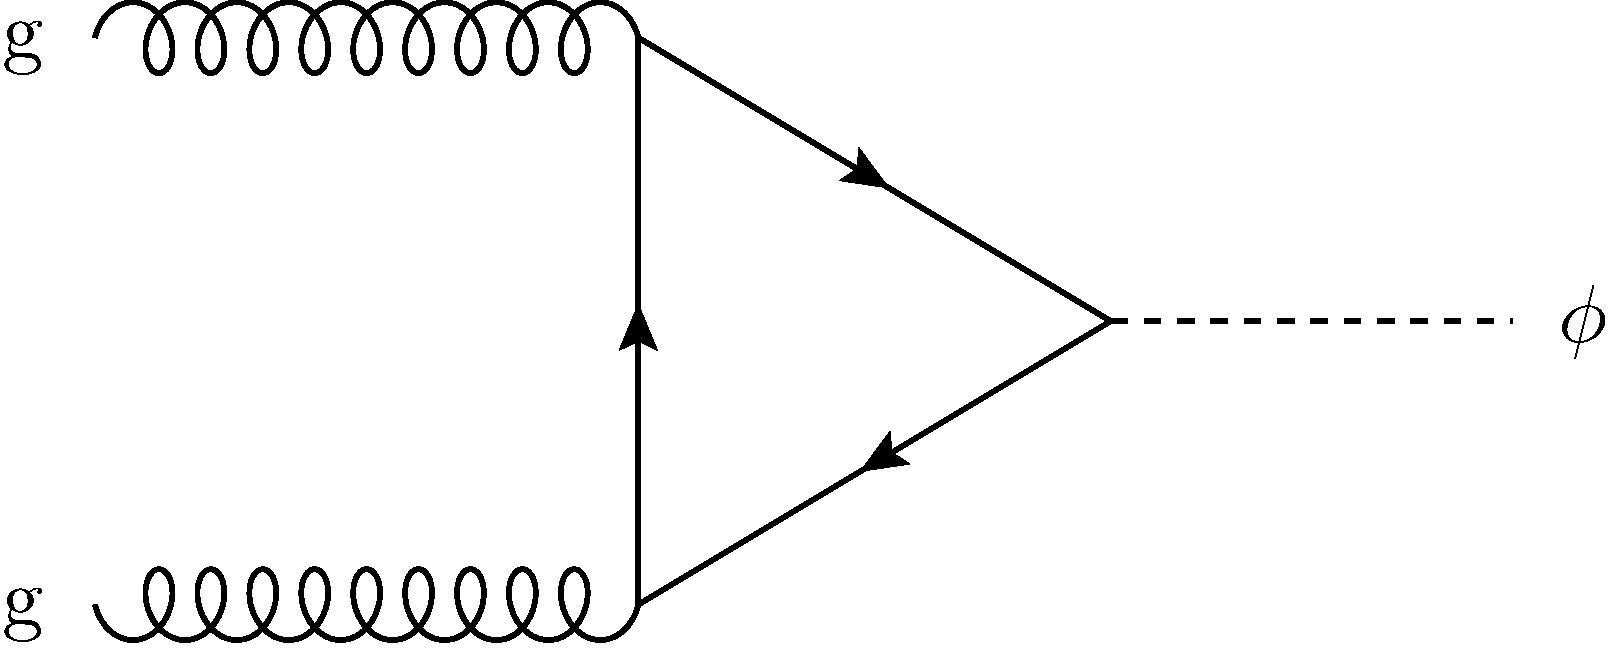
\includegraphics[width=0.55\textwidth]{plots/theory/feynman_mssm_ggH.pdf}}
\subfloat[]{
   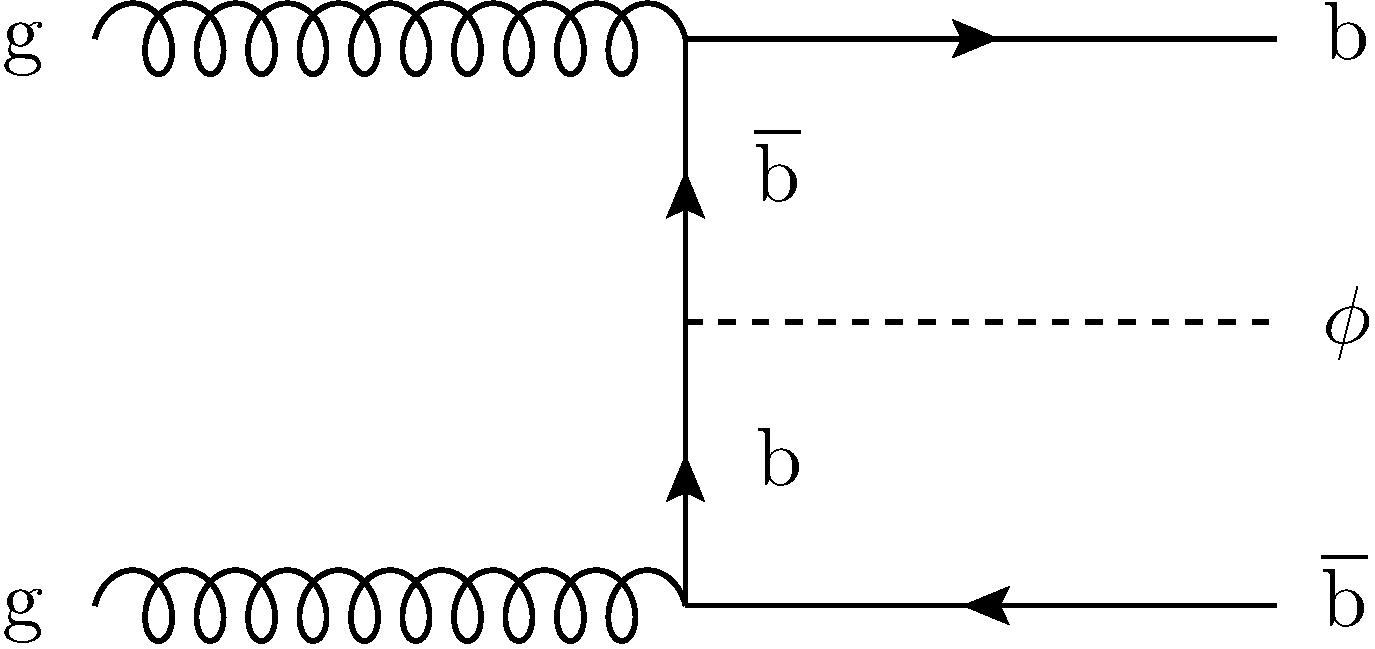
\includegraphics[width=0.45\textwidth]{plots/theory/feynman_mssm_bbH.pdf}}
\caption[Feynman diagrams illustrating example tree level production of neutral
Higgs bosons in the MSSM.]{Feynman diagrams illustrating example tree level production for the
gluon-fusion process (a) or b-assocated production process (b). The
particle $\Pphi$ indicates any one of the three neutral Higgs bosons, $\Ph$,
$\PH$ or $\PA$.}
\label{fig:mssmfeynman}
\end{figure}

\begin{figure}[htbp]
\subfloat[]{
   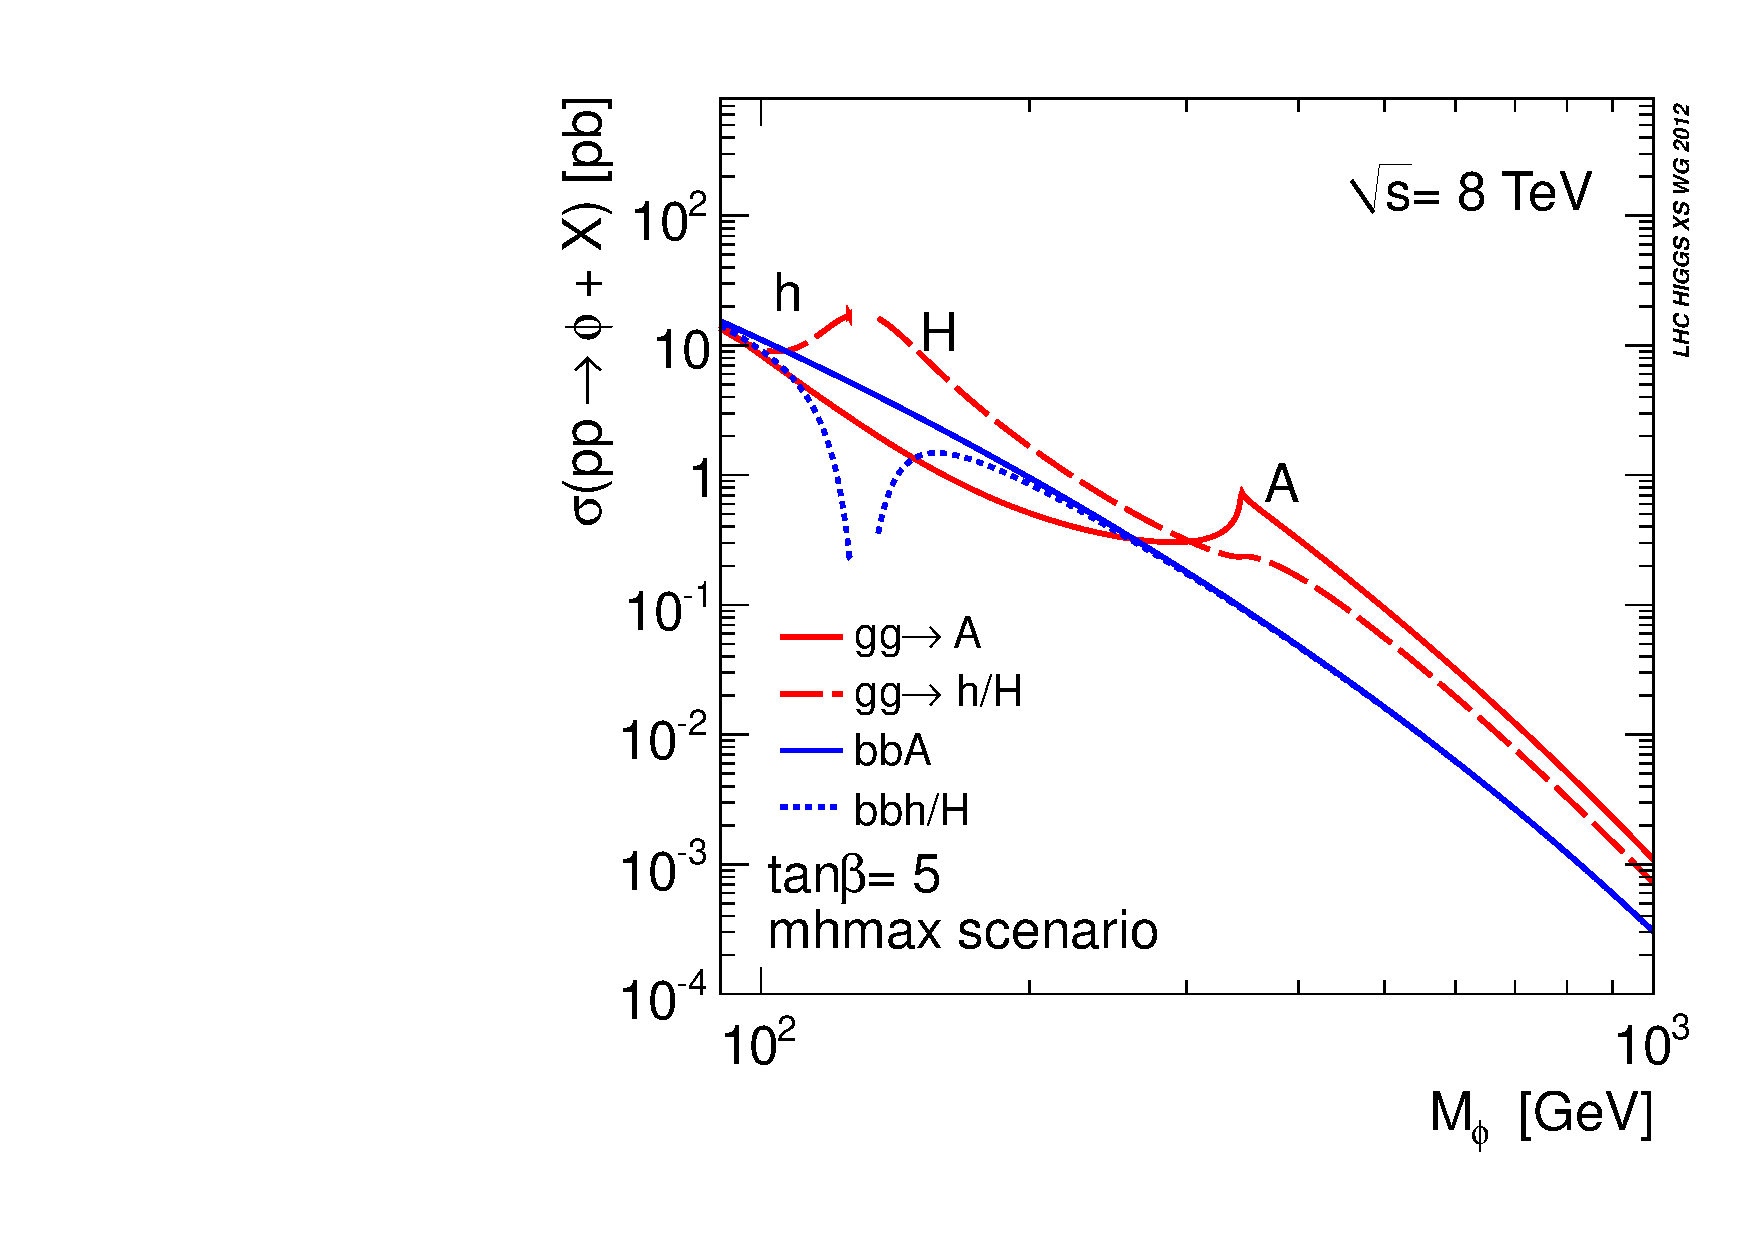
\includegraphics[width=0.5\textwidth]{plots/theory/YR3HXS_XSectSummary_mhmax8TeV_tanbeta5.pdf}}
\subfloat[]{
   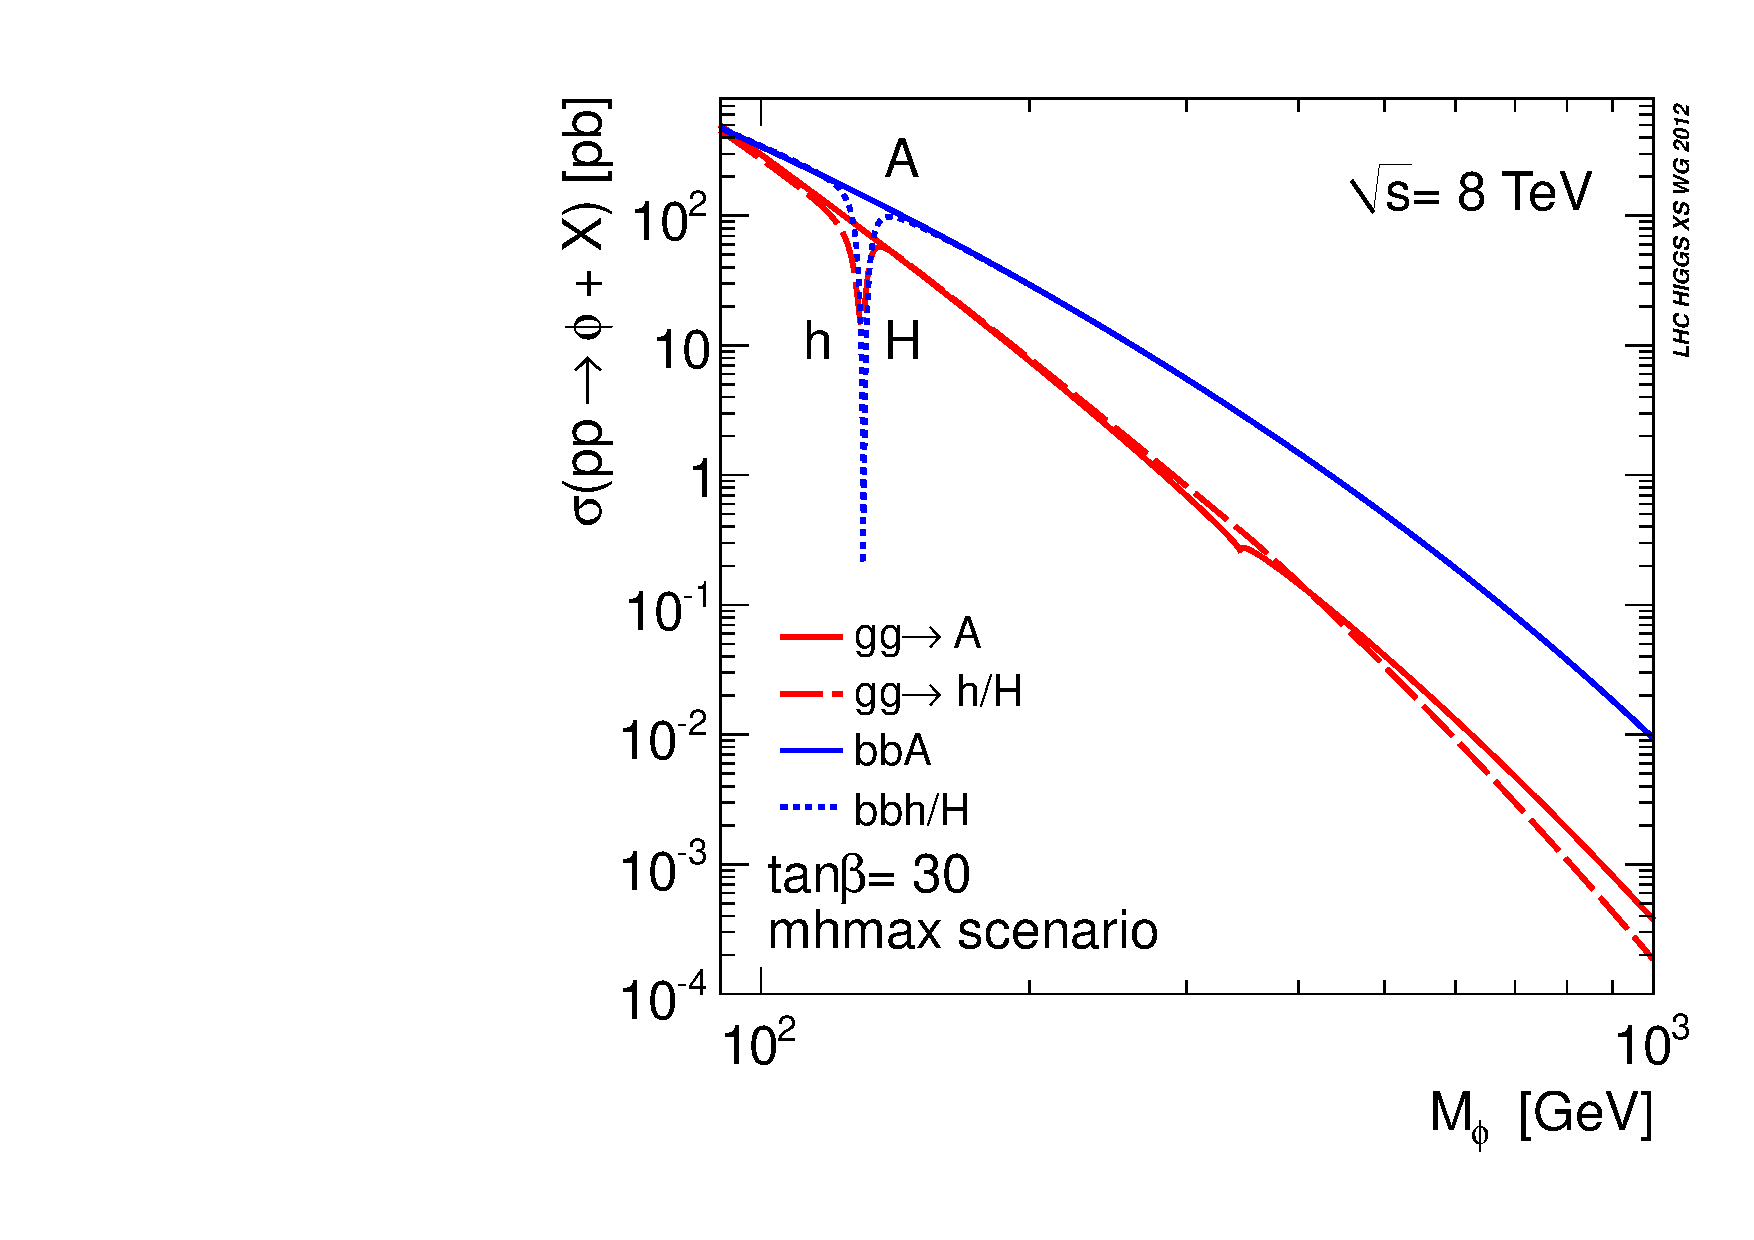
\includegraphics[width=0.5\textwidth]{plots/theory/YR3HXS_XSectSummary_mhmax8TeV_tanbeta30.pdf}}
\caption[Cross-sections for the production of neutral MSSM Higgs bosons in the 
$m_{\Ph}^{\text{max}}$ scenario.]{Cross-sections for the production of neutral MSSM Higgs bosons in the 
$m_{\Ph}^{\text{max}}$ scenario for $\tan\beta=5$ (a) and $\tan\beta=30$
(b) \cite{Heinemeyer:2013tqa}.}
\label{fig:mhmaxXSs}
\end{figure}

Previous searches for neutral \ac{MSSM} Higgs bosons were conducted at LEP, with
interpretation in the $m_{\Ph}^{max}$ scenario~\cite{Schael:2006cr}.
The results were negative and yielded limits $m_{\PA} > 93.4\,\GeV$ at $95\%$ CL.  
Results from the Tevatron~\cite{Benjamin:2010xb} provide complementary exclusion 
limits at high $\tan\beta$, considering masses up to $m_{\PA}=200\,\GeV$. The
higher centre of mass energy of the LHC provides access to $m_{\PA}$ values as
high as $1\,\TeV$. The most recent results from the LHC exclude large regions of
previously unreachable phase space in the $m_{h}^{\text{max}}$ scenario
\cite{Aad:2014vgg,HIG-13-021}. The results discussed in
chapter~\ref{chap:htt-mssm} follow those in \cite{HIG-13-021}.

\section{MSSM models incorporating the LHC Higgs boson}
\label{sec:mssmbenchmarks}

With the discovery of a 125$\,\GeV$ Higgs-like particle at the LHC, the number of
possible \ac{MSSM} scenarios is reduced to those which can incorporate this boson
with its measured properties. This section details some possible \ac{MSSM} scenarios
which can incorporate this 125$\,\GeV$ boson, whilst also exhibiting interesting
phenomenology motivated by experimental measurements. In particular the
scenarios must fulfil the condition $m_{\PH} = 125 \pm 3\,\GeV$ over a wide range
of parameter space, and satisfy the boundaries set by previous searches at LEP,
the Tevatron and the LHC. The $3\,\GeV$ uncertainty on the Higgs mass is
dominated by theoretical uncertainties in the \ac{MSSM} models. All of the scenarios 
considered are defined without allowing CP violation. The scenarios follow those
described in~\cite{MSSMScenarios}, with some small modifications. More detail
can be found in~\cite{HIG-13-021}, where these scenarios are discussed in the context
of the \ac{MSSM} $\Pphi \to \Pgt\Pgt$ analysis. 

As described previously, at tree level the masses of the five Higgs bosons are
defined by $m_{\PA}$ and $\tan\beta$. These masses are adjusted via radiative
corrections, necessary to produce a Higgs with mass consistent with $125\,\GeV$.
The parameters of interest in these radiative corrections are as follows:

\begin{itemize}
\item The mass of the top quark, $m_{\Pqt}$.
\item The mass of the bottom quark, $m_{\Pqb}$.
\item The mass of the 3rd generation squarks: stops and sbottoms, given by
$M_{\text{SUSY}}$.
\item The higgsino mass parameter, $\mu$.
\item The mass of the 3rd generation sleptons: the staus, given by
$M_{\PSlepton_{3}}$.
\item The $U(1)$ gaugino mass parameter, $M_{1}$.
\item The $SU(2)$ gaugino mass parameter, $M_{2}$.
\item The trilinear couplings of the stops, sbottoms and staus, $A_{\Pqt}$,
$A_{\Pqb}$ and $A_{\Pgt}$.
\item The mixing parameters of the stops, sbottoms and staus, $X_{\Pqt}$,
$X_{\Pqb}$ and $X_{\Pgt}$.
\end{itemize}

The dependence on these parameters can be reduced by exploiting relations
between them. For most scenarios, $M_{1}$ and $M_{2}$ are assumed to be related
at the GUT scale as:

\begin{equation}
M_{1} = \frac{5}{3}\frac{{\sin{\theta_{W}}}^{2}}{{\cos{\theta_{W}}}^{2}} M_{2},
\label{eq:GUTrelation}
\end{equation}

%with $\sin{\theta_{W}} = \sqrt{1-{\cos{\theta_{W}}}^{2}}$ and 
%$\cos{\theta_{W} = \frac{m_{W}}{m_{Z}}}$. 
Also the mixing parameters $X_{i}$ ($i=\Pqt$,$\Pqb$ or
$\Pgt$), the trilinear couplings $A_{i}$ and the higgsino mass parameter $\mu$ 
are related to the off-diagonal elements of the mixing matrices in the
stop, sbottom or stau sector as:
\begin{equation}
X_{\Pqt} = A_{\Pqt} -\mu\cot\beta, \quad X_{\Pqb} = A_{\Pqb} -\mu\tan\beta,
\quad X_{\Pgt} = A_{\Pgt} -\mu\tan\beta .
\end{equation}

Thus the list of parameters upon which the following \ac{MSSM} scenarios depend is
reduced to: $m_{\PA}$, $\tan\beta$, $m_{\Pqt}$, $m_{\Pqb}$, $M_{\text{SUSY}}$,
$\mu$, $M_{\PSlepton_{3}}$, $M_{2}$, $A_{\Pqt}$, $A_{\Pqb}$, $A_{\Pgt}$ and
$X_{\Pqt}$. Finally the following parameters have only a very small effect on
the \ac{MSSM} Higgs boson sector, and are fixed at chosen values which are compatible
with the current exclusion limits in direct searches:

\begin{itemize}
\item Masses of the first and second generation squarks, $M_{\Psquark_{1,2}} =
1500\,\GeV$.
\item Masses of the first and second generation sleptons, $M_{\PSlepton_{1,2}}
= 500\,\GeV$.
\item Trilinear couplings of the first and second generation squarks and
leptons, $A_{f} = 0$.
\end{itemize}

A summary of the scenarios considered is given in table
\ref{tab:mssmbenchmarks}, and a short description of each is given in the
following sections.

\subsubsection{The $m_{h}^{\text{max}}$ scenario}
\label{sec:mhmaxscenario}

The $m_{h}^{\text{max}}$ scenario was already discussed in the previous section
as the benchmark used at LEP, the Tevatron and early LHC searches. 
In this scenario the ratio of the stop mixing parameter and the
masses of the third generation squarks is chosen equal to 2
($|X_{\Pqt}/M_{\text{SUSY}}| = 2$). This yields a value of
$m_{\Ph}\sim135\,\GeV$ and high $m_{\PA}$ and $\tan\beta$. 
In light of the $125\,\GeV$ boson discovery, this scenario becomes less relevant,
since there is only a small amount of parameter space where either scalar
Higgs mass is consistent with $125\,\GeV$. Figure~\ref{fig:mhmaxmass} indicates
the region ruled out by this mass constraint. 

\begin{figure}[htbp]
   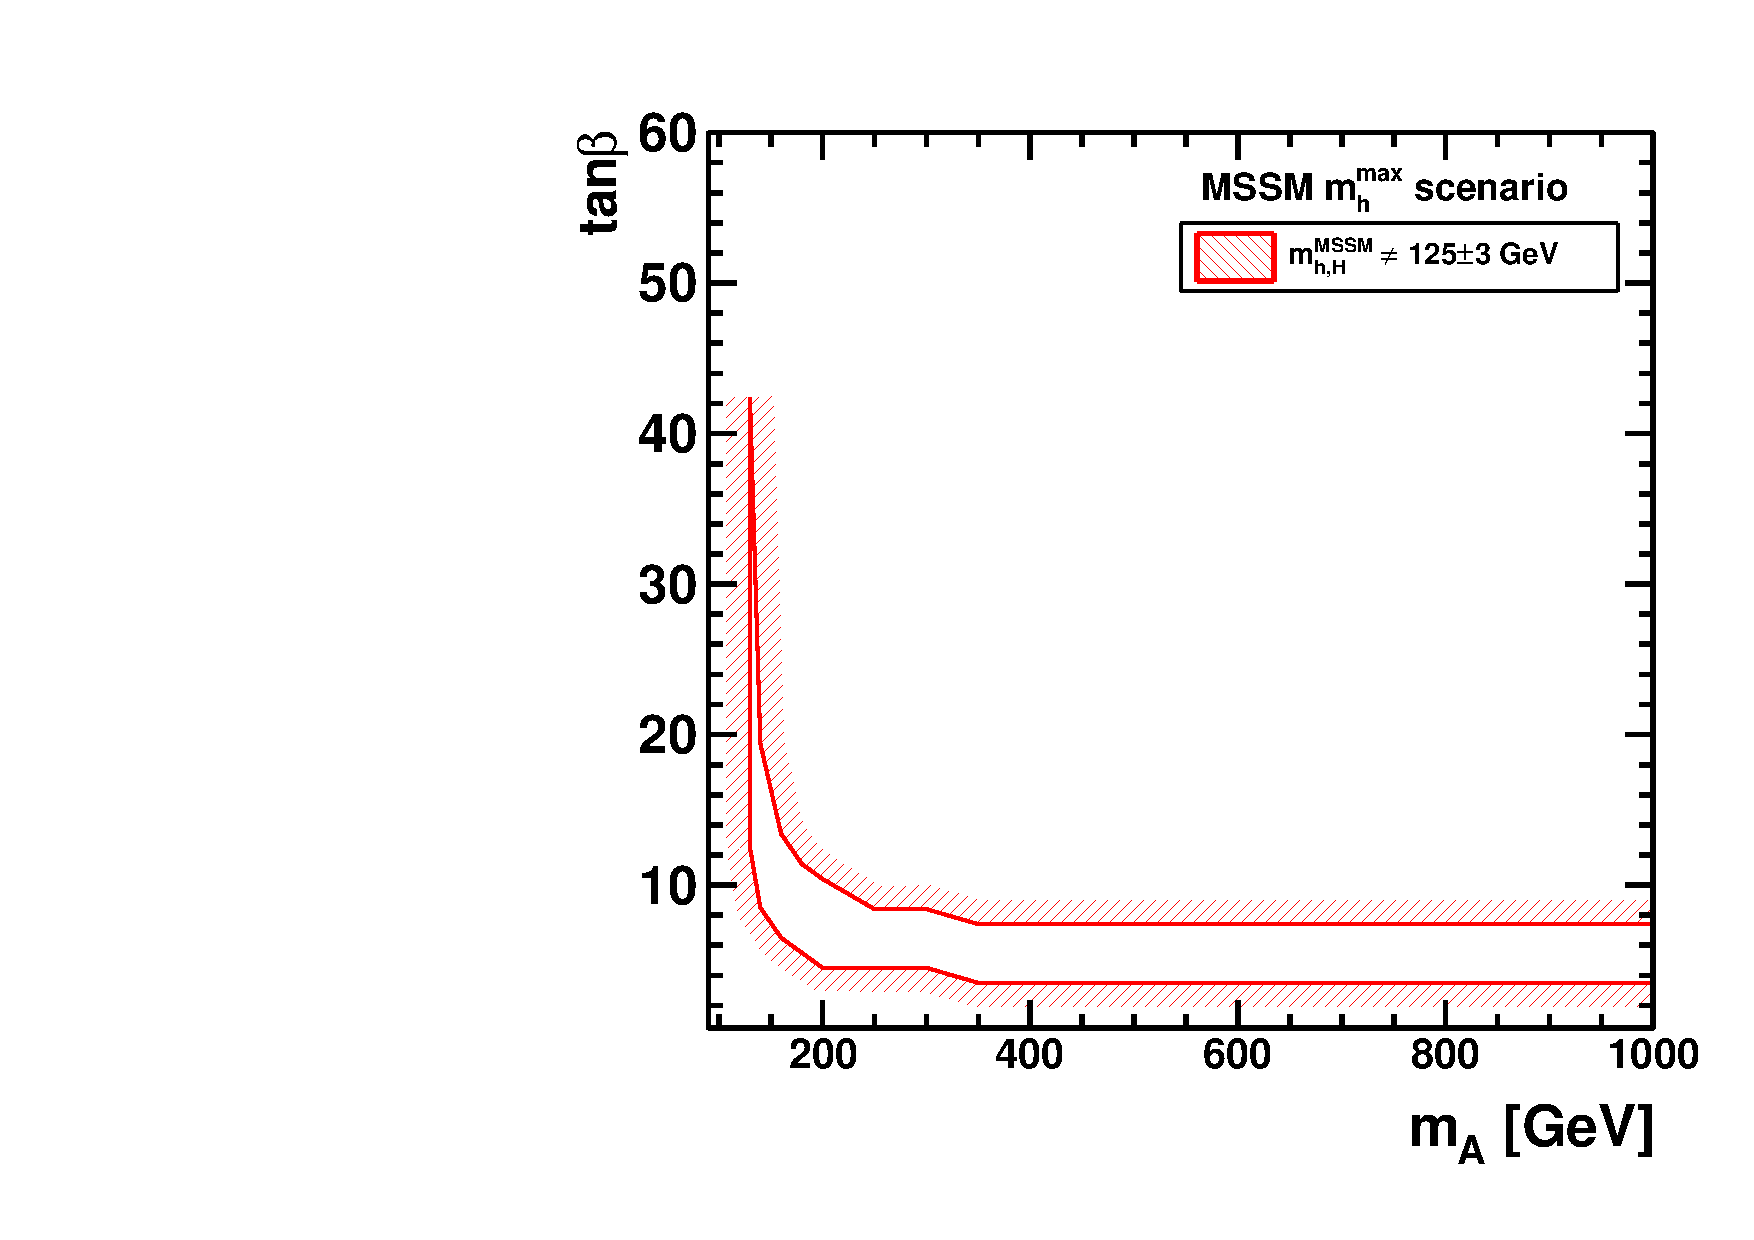
\includegraphics[width=0.5\textwidth]{plots/theory/cmb_mhmax-HypoTest.pdf}
\caption[Region of $m_{\PA}$-$\tan\beta$ space which yields a scalar Higgs mass 
consistent with $125\,\GeV$ in the $m_{h}^{\text{max}}$ scenario.]
{Region of $m_{\PA}$-$\tan\beta$ space which yields a scalar Higgs mass 
consistent with $125\,\GeV$ in the $m_{h}^{\text{max}}$ scenario. The majority of
this scenario is ruled out by the discovery of a 125$\,\GeV$ Higgs boson at the
LHC.}
\label{fig:mhmaxmass}
\end{figure}

\subsubsection{The $m_{h}^{\text{mod}}$ scenario}
\label{sec:mhmodscenario}

As the name suggests, the $m_{h}^{\text{mod}}$ is a slightly modified version of
the $m_{h}^{\text{max}}$, such that the mass of the light Higgs is consistent
with $125\,\GeV$ over a much wider range of phase space. This is achieved by
decreasing the ratio of the stop mixing parameter and the masses of the third
generation squarks, $|X_{\Pqt}/M_{\text{SUSY}}|$. In the $m_{h}^{\text{mod+}}$
scenario, the stop mixing is positive, $X_{\Pqt} = 1.5 \cdot M_{\text{SUSY}}$,
which gives better agreement with the experimental measurements of $(g-2)_{\mu}$
\cite{Miller:2007kk}. In the $m_{h}^{\text{mod-}}$ scenario, the stop mixing parameter is
negative, $X_{\Pqt} = -1.9 \cdot M_{\text{SUSY}}$, which results in a
\cal{B}($\Pqb\to\Pqs\Pphoton$) with better agreement with measurements
\cite{Lees:2012wg}.

Figure \ref{fig:mhmodmass} indicates the region of parameter space which yields
a Higgs consistent with $125\,\GeV$. It can be seen that the area is a lot larger
than in the $m_{h}^{\text{max}}$ case. In all subsequent scenarios, the allowed
region is very similar, excluding only very low $\tan\beta$ values. For the
other scenarios these allowed regions are shown in chapter~\ref{chap:htt-mssm},
in the context of the results of the \ac{MSSM} $\Pphi \to \Pgt\Pgt$ analysis which
are interpreted in these scenarios.

\begin{figure}[htbp]
\subfloat[]{
   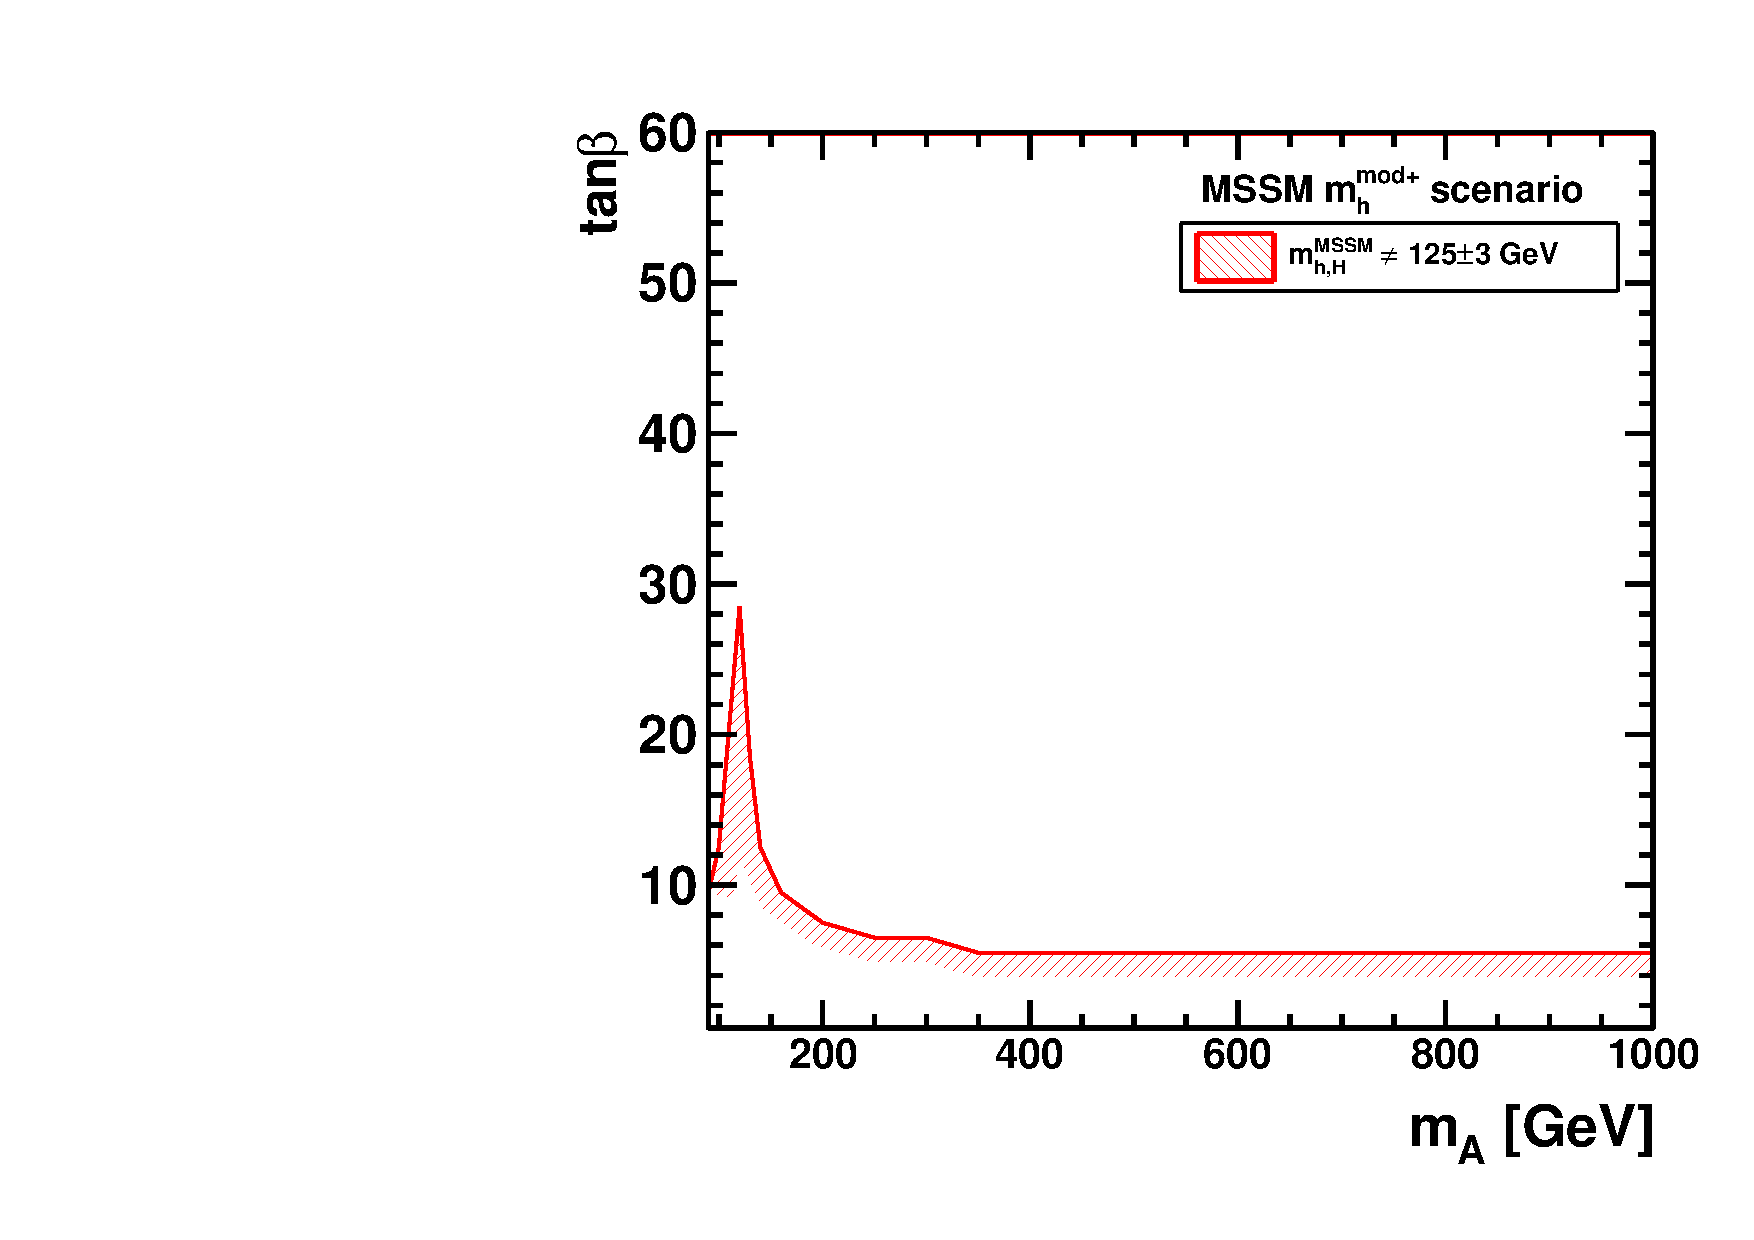
\includegraphics[width=0.5\textwidth]{plots/theory/cmb_mhmodp-HypoTest.pdf}}
\subfloat[]{
   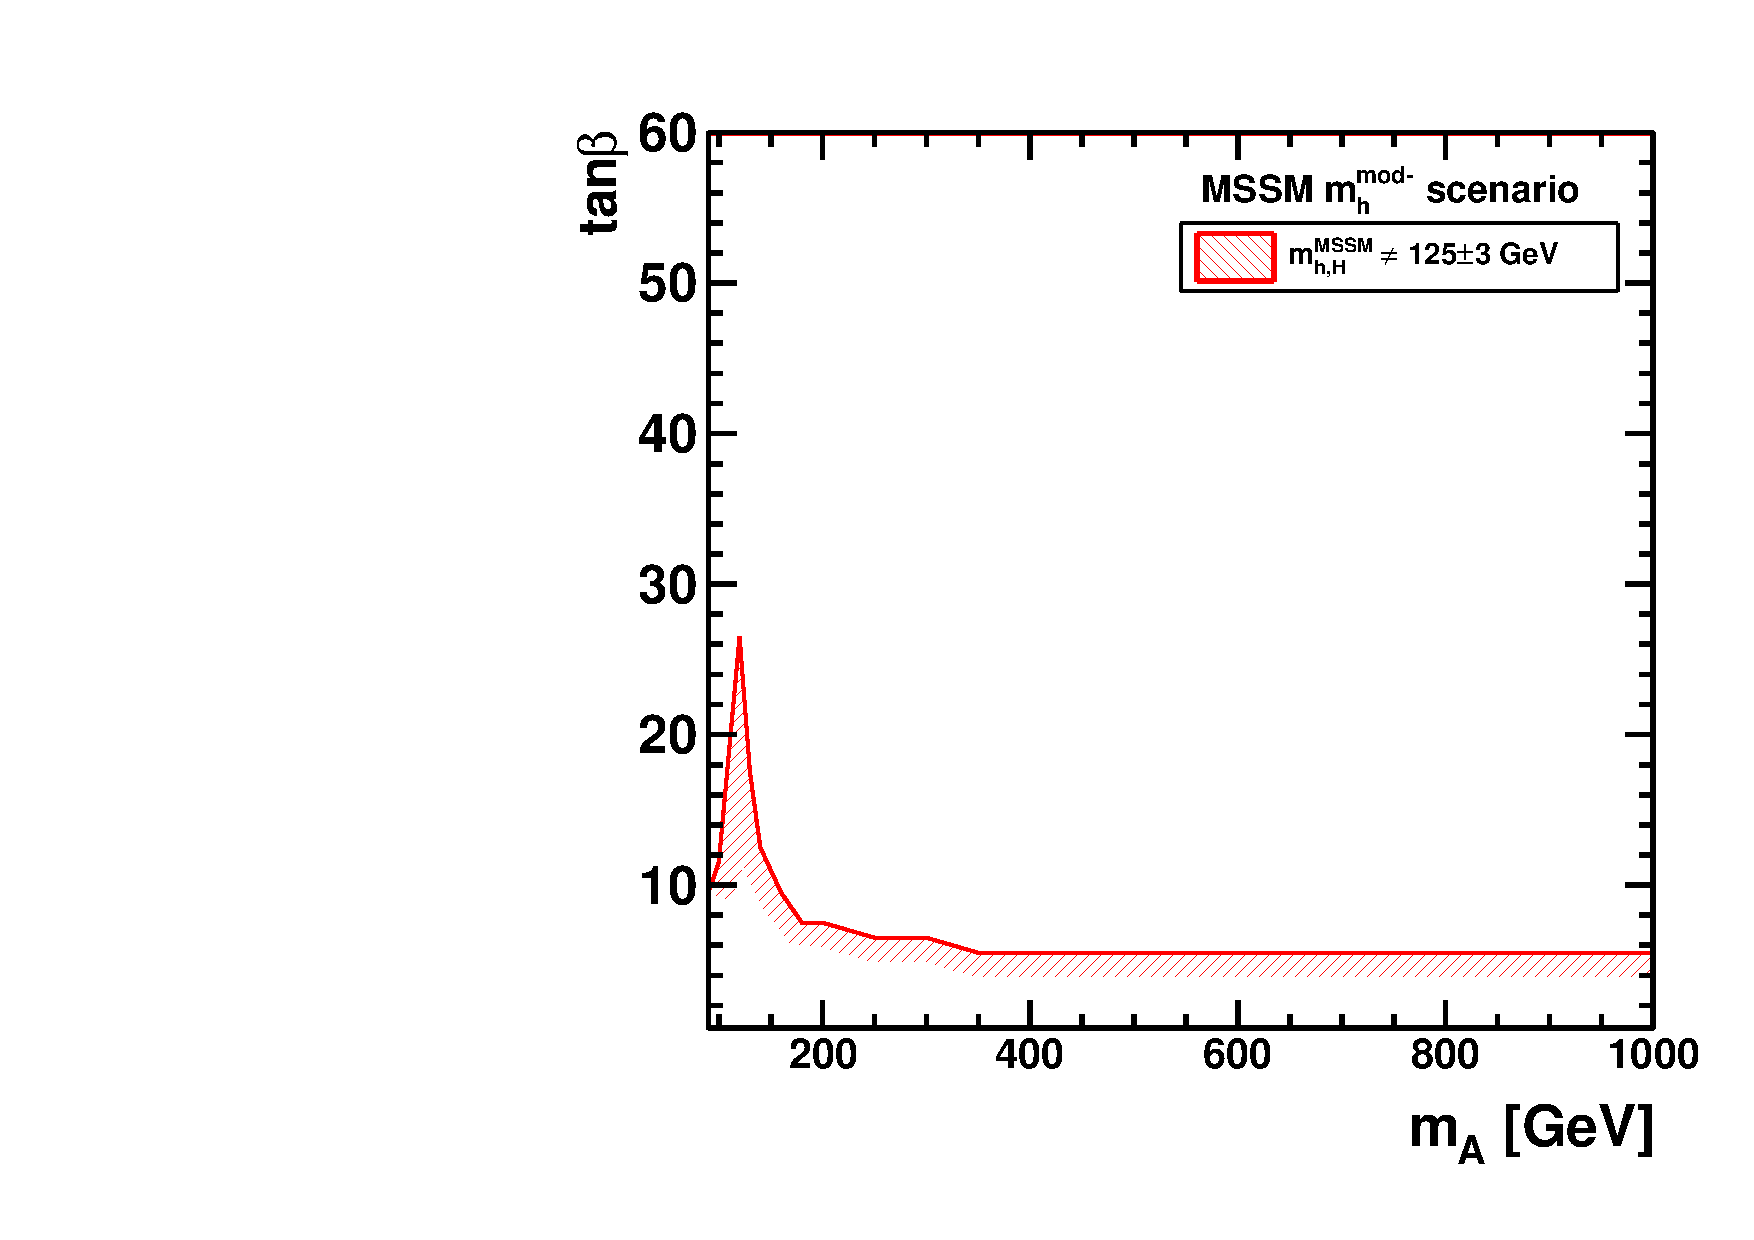
\includegraphics[width=0.5\textwidth]{plots/theory/cmb_mhmodm-HypoTest.pdf}}
\caption[Region of $m_{\PA}$-$\tan\beta$ space which yields a scalar Higgs mass 
consistent with $125\,\GeV$ in the $m_{h}^{\text{mod}}$ scenarios.]
{Region of $m_{\PA}$-$\tan\beta$ space which yields a scalar Higgs mass 
consistent with $125\,\GeV$ in the $m_{h}^{\text{mod+}}$ (a) and
$m_{h}^{\text{mod-}}$ (b) scenarios. In such modified scenarios, the
majority of phase space is consistent with the discovery of a $125\,\GeV$ Higgs.}
\label{fig:mhmodmass}
\end{figure}

\subsubsection{The light stop scenario}
\label{sec:lightstopscenario}

The mass of the lightest CP-even Higgs depends logarithmically on the stop mass,
and therefore a value of $125\,\GeV$ can be reached even with values of
$M_{\text{SUSY}} < 1\,\TeV$, provided the mixing in the stop sector is large. This
leads to light stops, which could modify the gluon-fusion Higgs production rate.
Such a scenario is referred to as the light-stop scenario. This scenario is
defined to be in agreement with current results of direct searches for stops.
Note that in this scenario $M_{1}$ and $M_{2}$ are not related by the GUT
relation in equation~\ref{eq:GUTrelation}. 
%An assumption used for the calculation of cross-sections in this scenario assumes
%that $m_{\PH} < 2\times $

\subsubsection{The light stau scenario}
\label{sec:lightstauscenario}

The light stau scenario is motivated by the excess of events in the decay
channel of the $\PH\to\Pphoton\Pphoton$ measured by ATLAS~\cite{ATLAS-CONF-2013-012}. 
Light staus lead to a modification of the ratio of the lightest Higgs boson decaying into
two photons with respect to the \ac{SM} expectation:
\begin{equation}
r_{\Pphoton\Pphoton} =
\frac{\Gamma(\Ph\to\Pphoton\Pphoton)_{\text{MSSM}}}{\Gamma(\Ph\to\Pphoton\Pphoton)_{\text{SM}}}
.
\end{equation}

For high values of $\tan\beta$ and $m_{\PA}$ this ratio can be as high as 1.3. 

\subsubsection{The $\Pgt$-phobic scenario}
\label{sec:tauphobicscenario}

Similarly to the case of the light stau scenario, the $\Pgt$-phobic scenario is
motivated by the possibility to allow reduced couplings to down-type fermions.
In high $\tan\beta$ and $m_{\PA}$, the ratios:
\begin{equation}
r_{\Pqb\Pqb} =
\frac{\Gamma(\Ph\to\Pqb\Pqb)_{\text{MSSM}}}{\Gamma(\Ph\to\Pqb\Pqb)_{\text{SM}}}
, \quad
r_{\Pgt\Pgt} =
\frac{\Gamma(\Ph\to\Pgt\Pgt)_{\text{MSSM}}}{\Gamma(\Ph\to\Pgt\Pgt)_{\text{SM}}}
\end{equation}

can be significantly lower than 1.

\subsubsection{The low-$m_{\PH}$ scenario}
\label{sec:lowmHscenario}

The low-$m_{\PH}$ scenario is somewhat different from the other scenarios due to
the fact that in this scenario, the Higgs boson with mass of $125\,\GeV$ is
assumed to be the heavier scalar Higgs $\PH$. This means that the mass of the
pseudoscalar Higgs must be chosen to be not too high, and is fixed at $m_{\PA} =
110\,\GeV$. Since $m_{\PA}$ is fixed in this scenario, the 2-D parameter space
for the scan is chosen as $\mu$-$\tan\beta$, with $\mu$ varied between 300 and
$3100\,\GeV$ and $\tan\beta$ between 1.5 and 9.5. All the other parameters are
very similar to those in the $\Pgt$-phobic scenario. In this scenario, the
couplings of the lightest Higgs boson $\Ph$ to gauge bosons is significantly
reduced compared with the \ac{SM} expectations by a factor 2-10, to ensure that
the \Ph is not already excluded by LEP limits. 

\begin{table}[tbh]
\begin{tabular}{|l|c|c|c|}
\hline
Parameter & $m_{h}^{\text{max}}$ & $m_{h}^{\text{mod+}}$ & $m_{h}^{\text{mod-}}$ \\
\hline
$m_{\PA}$ & $90-1000\,\GeV$ & $90-1000\,\GeV$ & $90-1000\,\GeV$\\
$\tan\beta$ & 0.5-60 & 0.5-60 & 0.5-60 \\
$M_{\text{SUSY}}$ & $1000\,\GeV$ & $1000\,\GeV$ & $1000\,\GeV$\\
$\mu$ & $200\,\GeV$ & $200\,\GeV$ & $200\,\GeV$\\
$M_{1}$ & $(5/3)M_{2}\tan{\theta_{W}}^{2}$ & $(5/3)M_{2}\tan{\theta_{W}}^{2}$ & $(5/3)M_{2}\tan{\theta_{W}}^{2}$\\
$M_{2}$ & $200\,\GeV$ & $200\,\GeV$ & $200\,\GeV$ \\
$X_{\Pgt}$ & $2M_{\text{SUSY}}$ & $1.5M_{\text{SUSY}}$ & $-1.9M_{\text{SUSY}}$ \\
$A_{\Pqb},A_{\Pqt},A_{\Pgt}$ & $A_{\Pqb} = A_{\Pqt} = A_{\Pgt}$ & $A_{\Pqb} = A_{\Pqt} = A_{\Pgt}$ & $A_{\Pqb} = A_{\Pqt} = A_{\Pgt}$\\
$m_{\PSgluino}$ & $1500\,\GeV$ & $1500\,\GeV$ & $1500\,\GeV$\\
$m_{\PSlepton_{3}}$ & $1000\,\GeV$ & $1000\,\GeV$ & $1000\,\GeV$\\
\hline
\end{tabular}
\begin{tabular}{|l|c|c|c|c|}
\hline
Parameter & light-stop & light-stau & $\Pgt$-phobic & low-$m_{\PH}$ \\
\hline
$m_{\PA}$ & $90-1000\,\GeV$ & $90-1000\,\GeV$ & $90-1000\,\GeV$ & $110\,\GeV$\\
$\tan\beta$ & 0.7-60 & 0.5-60 & 0.9-50 & 1.5-9.5\\
$M_{\text{SUSY}}$ & $500\,\GeV$ & $1000\,\GeV$ & $1500\,\GeV$ & $1500\,\GeV$\\
$\mu$ & $400\,\GeV$ & $500\,\GeV$ & $2000\,\GeV$ & $300-3100\,\GeV$\\
$M_{1}$ & $340\,\GeV$ & $(5/3)M_{2}\tan{\theta_{W}}^{2}$ & $(5/3)M_{2}\tan{\theta_{W}}^{2}$  & $(5/3)M_{2}\tan{\theta_{W}}^{2}$ \\
$M_{2}$ & $400\,\GeV$ & $200\,\GeV$ & $200\,\GeV$ & $200\,\GeV$\\
$X_{\Pgt}$ & $2M_{\text{SUSY}}$ & $1.6M_{\text{SUSY}}$ & $2.45M_{\text{SUSY}}$ & $2.45M_{\text{SUSY}}$ \\
$A_{\Pqb},A_{\Pqt},A_{\Pgt}$ & $A_{\Pqb} = A_{\Pqt} = A_{\Pgt}$ & $A_{\Pqb} = A_{\Pqt}, A_{\Pgt} = 0$ & $A_{\Pqb} = A_{\Pqt} = A_{\Pgt}$ & $A_{\Pqb} = A_{\Pqt} = A_{\Pgt}$ \\
$m_{\PSgluino}$ & $1500\,\GeV$ & $1500\,\GeV$  & $1500\,\GeV$ & $1500\,\GeV$ \\
$m_{\PSlepton_{3}}$ & $1000\,\GeV$ & $245\,\GeV$ & $500\,\GeV$ &  $1000\,\GeV$ \\
\hline
\end{tabular}
\caption[Parameters defining the $m_{h}^{\text{max}}$, $m_{h}^{\text{mod+}}$,
$m_{h}^{\text{mod-}}$, light-stop, light-stau, $\Pgt$-phobic and
low-$m_{\PH}$ MSSM benchmark scenarios.]{Parameters defining the $m_{h}^{\text{max}}$, $m_{h}^{\text{mod+}}$,
$m_{h}^{\text{mod-}}$, light-stop, light-stau, $\Pgt$-phobic and
low-$m_{\PH}$ MSSM benchmark scenarios \cite{HIG-13-021}.}
\label{tab:mssmbenchmarks}
\end{table}

\subsection{Modification of MSSM models at low $\tan\beta$}
\label{sec:lowtanbscenario}

In all of the scenarios discussed in the previous sections, the mass of either
the lighter or heavier scalar Higgs boson is consistent with $125\,\GeV$ over a
wide range of phase space. However, one thing common to all of these scenarios
is the fact that in general the mass is not consistent at very low $\tan\beta$
values, where the mass of the lightest Higgs becomes too light to be consistent
with $125\,\GeV$. As results such as those discussed in chapter~\ref{chap:htt-mssm} 
rule out larger regions of phase space at high $\tan\beta$, attention turns to this low
$\tan\beta$ region and analyses which could access it.

The low $\tan\beta$ region can be re-opened if the value of $M_{\text{SUSY}}$ is
allowed to be higher than $1\,\TeV$~\cite{Djouadi:2013vqa}. In the \ac{MSSM}, values of
$M_{\text{SUSY}}$ must be lower than $3\,\TeV$ to avoid too much fine tuning in
the model. However, as searches at the LHC have yet to discover supersymmetric
particles, it is natural that models with higher \ac{SUSY} scales are being
considered, and as the allowed amount of fine-tuning in a model is somewhat
subjective, attention is turning more to these types of scenarios. Figure
\ref{fig:MSUSYcontours} illustrates the mass of the $\Ph$ boson at different
choices of $M_{\text{SUSY}}$ for a range of $\tan\beta$ values. It can be seen
that $m_{\Ph} = 125\pm 3\,\GeV$ can be achieved for values of $\tan\beta$ as low
as $1\,\GeV$ if $M_{\text{SUSY}}$ is allowed to be in the range $100-1000\,\TeV$.
Slightly higher $\tan\beta$ values in the range 2--5 can be achieved with
$M_{\text{SUSY}}$ values only as high as a few $\TeV$. 

\begin{figure}[htbp]
   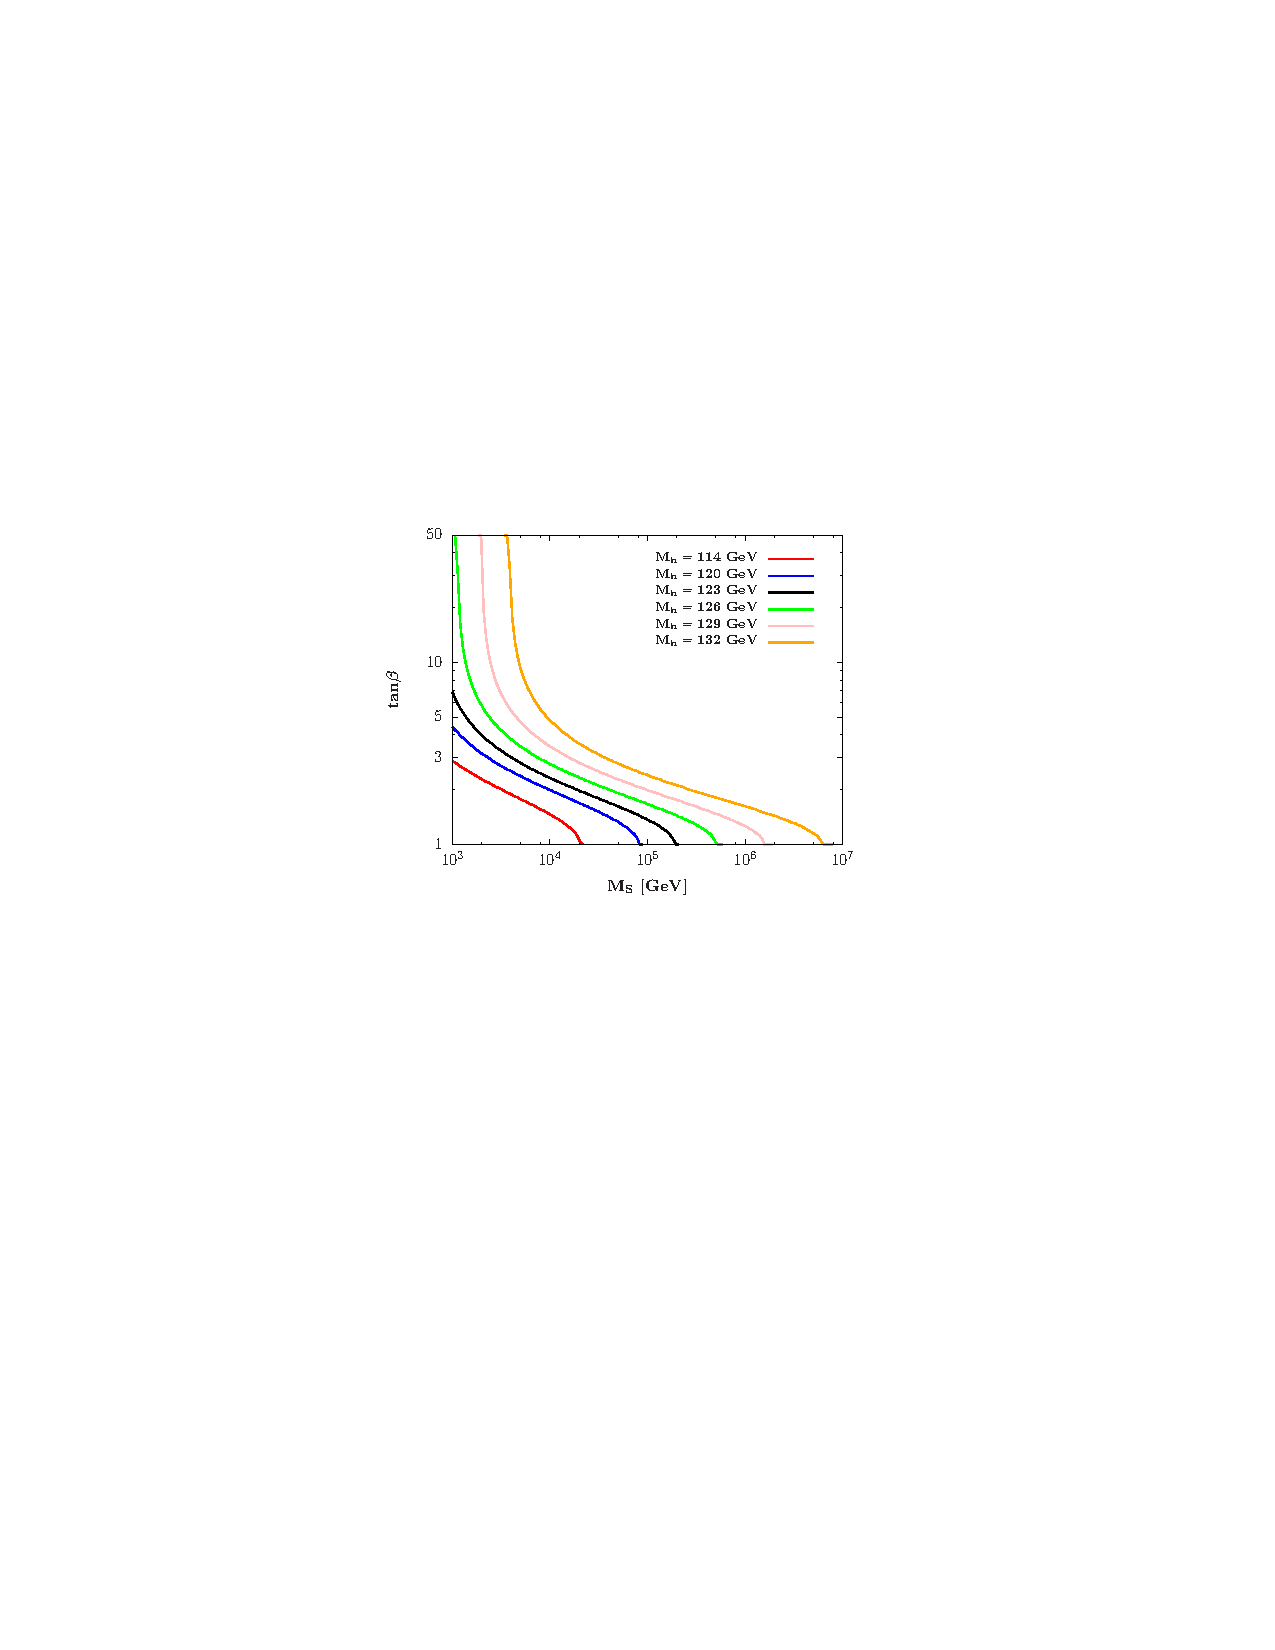
\includegraphics[width=0.7\textwidth]{plots/theory/MSUSY_tanb.pdf}
\caption[Contours in the $M_{\text{SUSY}}$-$\tan\beta$ plane for
constant $m_{\Ph}$ values around $125\,\GeV$.]{Contours in the $M_{\text{SUSY}}$($M_{S}$)-$\tan\beta$ plane for
constant $m_{\Ph}$ values around $125\,\GeV$, illustrating that higher
$M_{\text{SUSY}}$ values can allow a light Higgs consistent with $125\,\GeV$ for
even very low $\tan\beta$ values \cite{Djouadi:2013vqa}.}
\label{fig:MSUSYcontours}
\end{figure}

In such a low $\tan\beta$ region, the gluon fusion production process dominates
over any b-associated production. Figure~\ref{fig:XSlowtanb} indicates the
production cross-sections for each of the neutral Higgs bosons in such a low
$\tan\beta$ regime for $\sqrt{s}=8\,\TeV$. It can be seen that the production of
the heavier $\PA$ and $\PH$ bosons via gluon fusion dominates over any of the
other production mechanisms. Thus to access information about such a scenario,
the heavier Higgs bosons with masses up to $1\,\TeV$ must be searched for.
Figure~\ref{fig:BRlowtanb} illustrates the branching ratios of the $\PA$ and
$\PH$ bosons in such a mass range. 

\begin{figure}[htbp]
   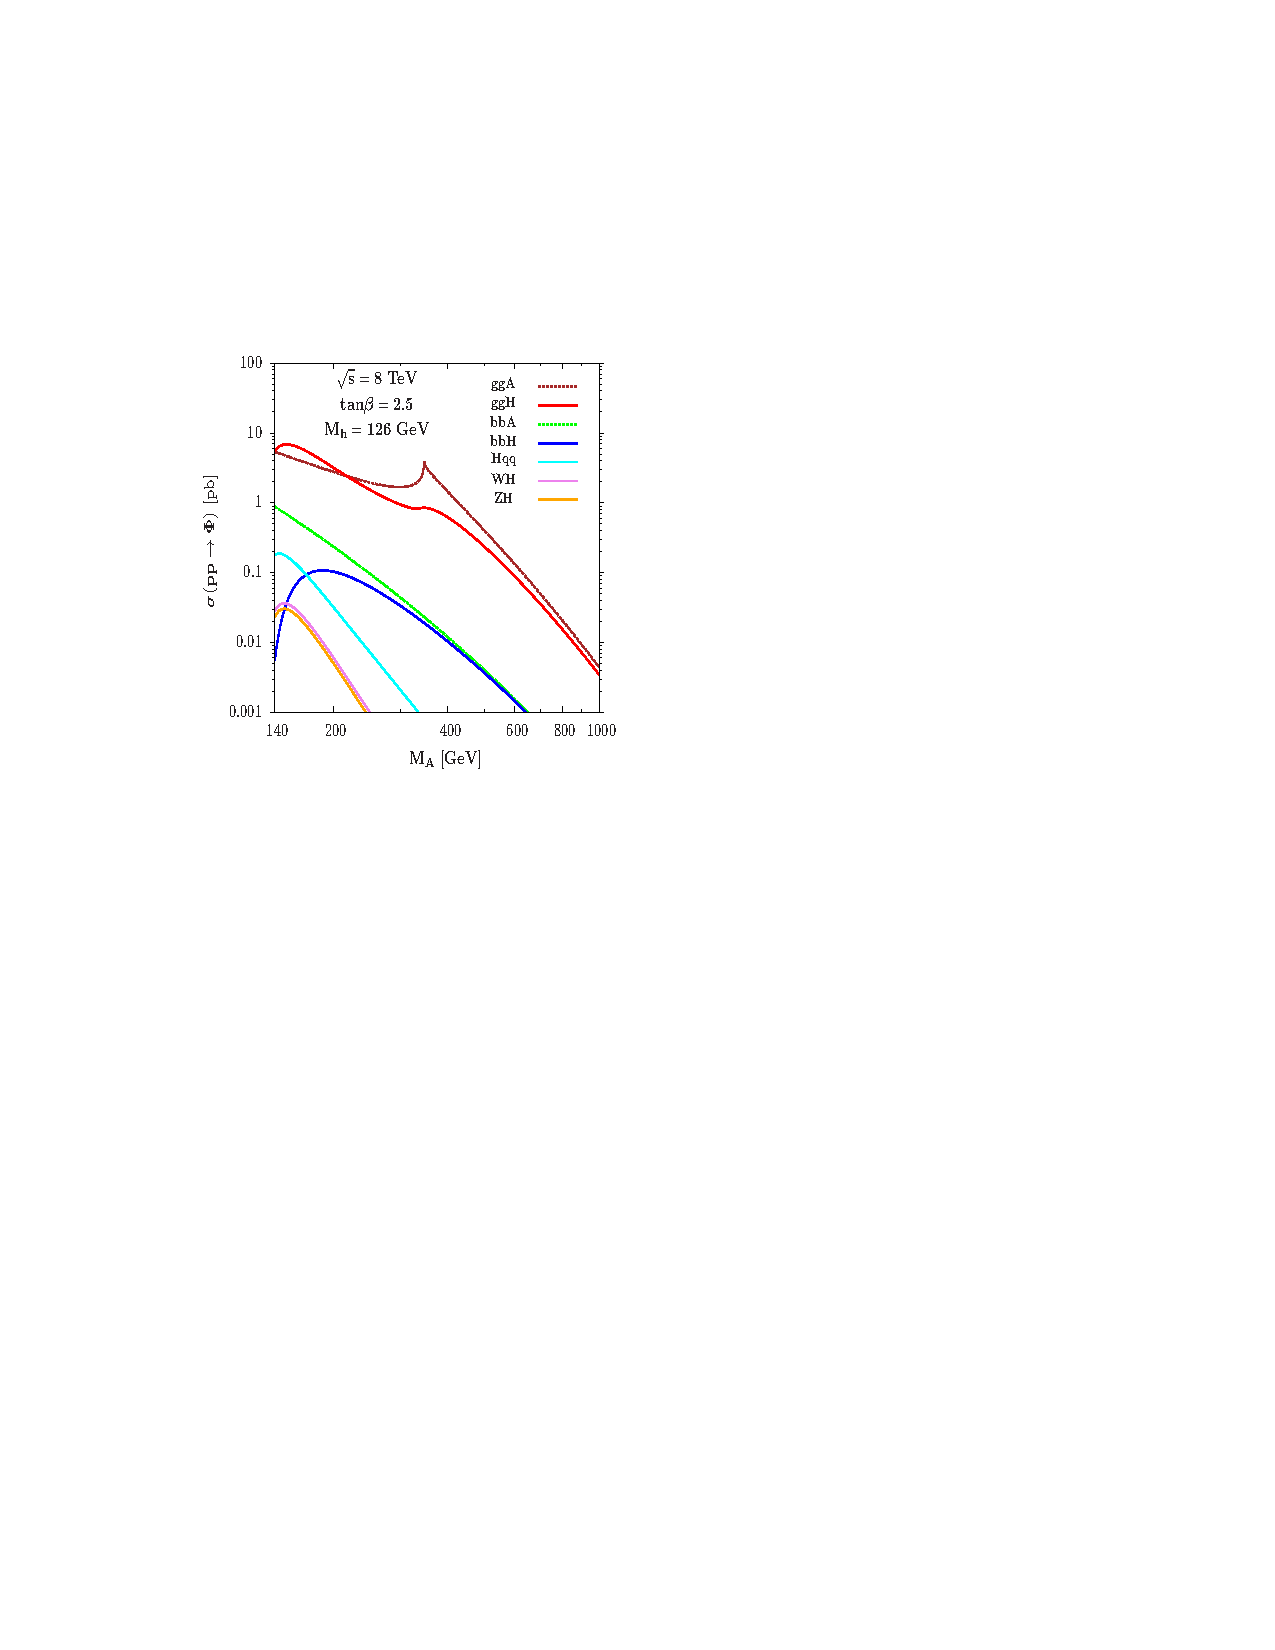
\includegraphics[width=0.5\textwidth]{plots/theory/XS_lowtanb.pdf}
\caption[Cross-sections for the production of the three neutral Higgs bosons in
the low $\tan\beta$ regime.]{Cross-sections for the production of the three neutral Higgs bosons in
the low $\tan\beta$ regime. The production of the $\PH$ and $\PA$ bosons
via gluon fusion dominates over any of the other production processes~\cite{Djouadi:2013vqa}.}
\label{fig:XSlowtanb}
\end{figure}

\begin{figure}[htbp]
   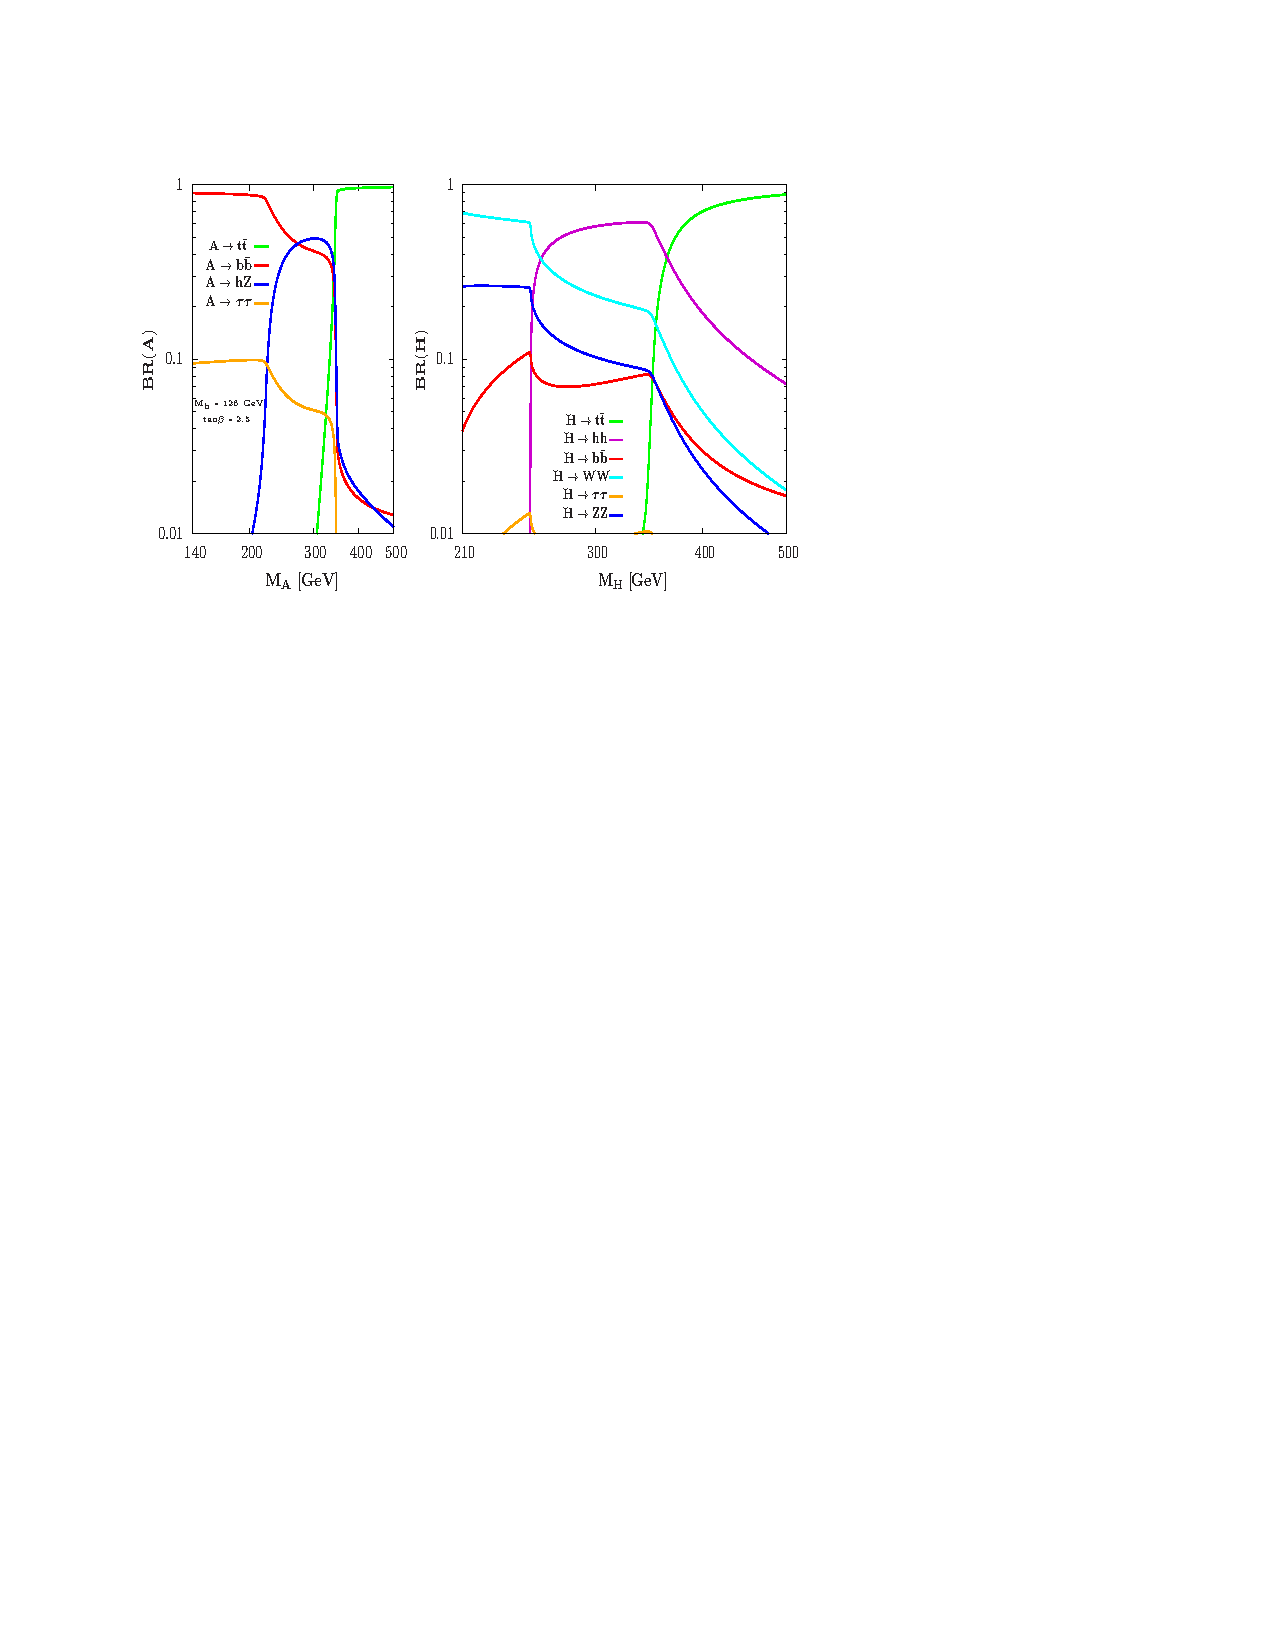
\includegraphics[width=0.7\textwidth]{plots/theory/BR_lowtanb.pdf}
\caption[Branching ratios for the $\PH$ and $\PA$ bosons in the low $\tan\beta$
regime.]{Branching ratios for the $\PH$ and $\PA$ bosons in the low $\tan\beta$
regime, for $\tan\beta=2.5$~\cite{Djouadi:2013vqa}.}
\label{fig:BRlowtanb}
\end{figure}

From figure \ref{fig:BRlowtanb}, it can be seen that in the central region of 
$m_{\PA}-\tan\beta$ space, branching ratios for the decays of
$\PH\to\Ph\Ph$ and $\PA\to\PZ\Ph$ are enhanced. Several recent LHC analyses have
made searches for these decays in the scenario where the $\Ph$ is the $125\,\GeV$
Higgs discovered at the LHC. Various final states have been studied including
for the $\PH\to\Ph\Ph$ analysis $\Pphoton\Pphoton\Pqb\Pqb$ \cite{Aad:2014yja,CMS-PAS-HIG-13-032} and 
$\Pqb\Pqb\Pqb\Pqb$ \cite{CMS-PAS-HIG-14-013} and for the $\PA\to\PZ\Ph$ analysis $\ell\ell\Pqb\Pqb$
and $\ell\ell\Pgt\Pgt$ \cite{Aad:2015wra,CMS-PAS-HIG-14-011}. 
Chapter~\ref{chap:Hhh} documents a $\PH\to\Ph\Ph$ analysis in the
final state of $\Pgt\Pgt\Pqb\Pqb$. Such results can be interpreted in an
appropriate low $\tan\beta$ scenario.

\subsubsection{The low-$\tan\beta$-high scenario}
\label{sec:lowtanbscenario}

An appropriate \ac{MSSM} scenario at low $\tan\beta$ is known as the
low-$\tan\beta$-high scenario~\cite{lowtanbhighwiki}. Such a scenario depends on radiative
corrections like those described previously. To attain a light Higgs boson mass
consistent with $125\pm3\,\GeV$ for low-$\tan\beta$ values in the range 0.5-4,
$M_{\text{SUSY}}$ is varied between $1$-$100\,\TeV$ and the parameter $X_{\Pqt}$ is
varied such that:

%\begin{align}
%\begin{array}{ll}

%\text{for $\tan\beta\leq2$} & |X_{\Pqt}/M_{\text{SUSY}}| = 2 \\ 
%\text{for $2<\tan\beta\leq8.6$} & |X_{\Pqt}/M_{\text{SUSY}}| =
%0.0375\tan^{2}\beta - 0.7\tan\beta + 3.25 \\
%\text{for $8.6<\tan\beta$} & |X_{\Pqt}/M_{\text{SUSY}}| = 0 \\

%\end{array}
%\end{align}

\begin{align*}
%\Delta R =
%  \left\{
    \begin{array}{ll}
        \text{for $\tan\beta\leq2$}: & |X_{\Pqt}/M_{\text{SUSY}}| = 2 \\
        \text{for $2<\tan\beta\leq8.6$}:  & |X_{\Pqt}/M_{\text{SUSY}}| = 0.0375\tan^{2}\beta - 0.7\tan\beta + 3.25  \\
        \text{for $8.6<\tan\beta$}: & |X_{\Pqt}/M_{\text{SUSY}}| = 0 \\ 
    \end{array}
%  \right.
\end{align*}

%\begin{equation}
%\text{for $\tan\beta\leq2$},\ |X_{\Pqt}/M_{\text{SUSY}}| = 2 \\
%\text{for $2<\tan\beta\leq8.6$},\ |X_{\Pqt}/M_{\text{SUSY}}| =
%0.0375\tan^{2}\beta - 0.7\tan\beta + 3.25  \\
%\text{for $8.6<\tan\beta$},\ |X_{\Pqt}/M_{\text{SUSY}}| = 0  \\
%\end{equation}

All other trilinear couplings are set to $2000\,\GeV$, $\mu=1500\,\GeV$ and
$M_{2}=2000\,\GeV$. With these choices, the region of $m_{\PA}-\tan\beta$ space
consistent with the $125\,\GeV$ mass is as shown in
figure~\ref{fig:lowtanbhighmass}.

\begin{figure}[htbp]
   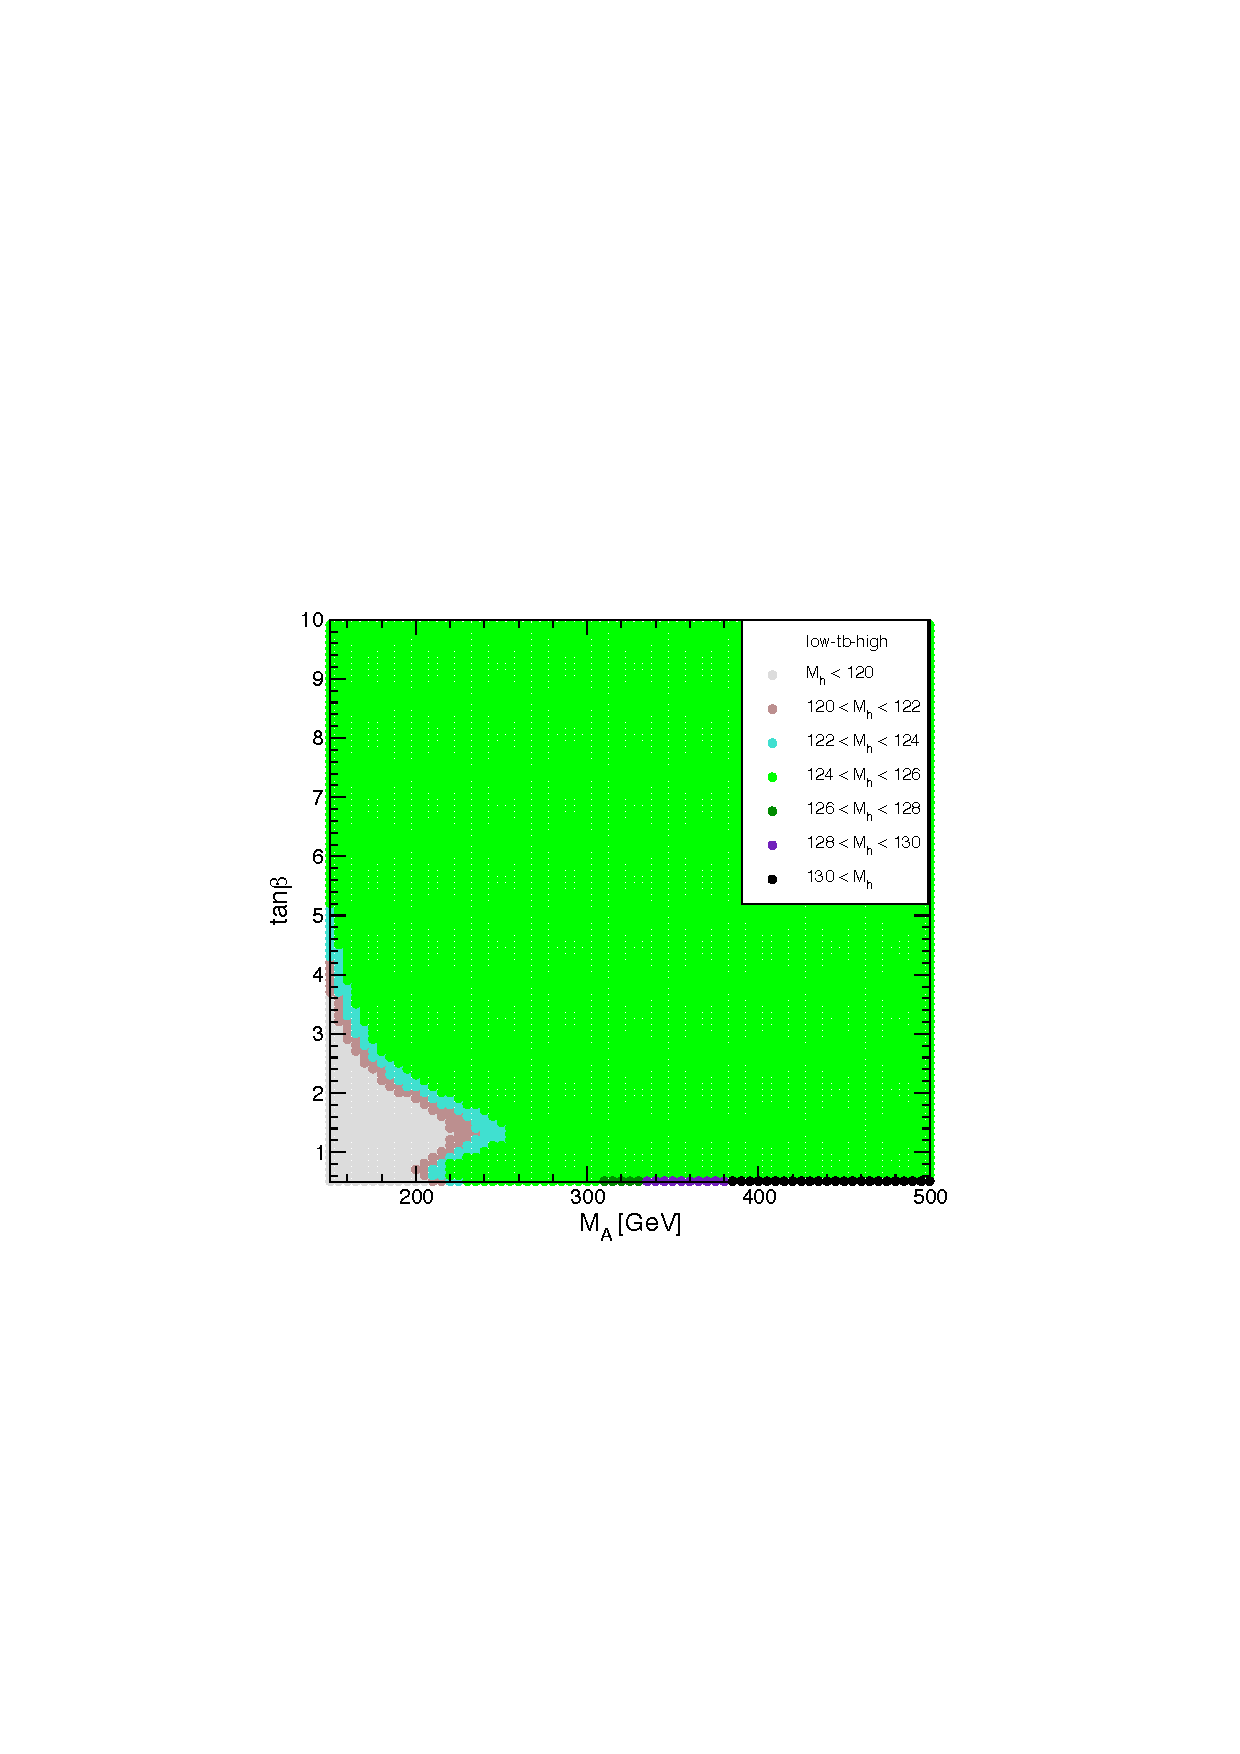
\includegraphics[width=0.5\textwidth]{plots/theory/low-tanb-high-mass.pdf}
\caption[Region of $m_{\PA}$-$\tan\beta$ space which yields a scalar Higgs mass 
consistent with $125\,\GeV$ in the low-$\tan\beta$-high scenario.]{
    Region of $m_{\PA}$-$\tan\beta$ space which yields a scalar Higgs mass 
consistent with $125\,\GeV$ in the low-$\tan\beta$-high scenario. The
majority of phase space is consistent with the discovery of a $125\,\GeV$ Higgs
boson~\cite{lowtanbhighwiki}.}
\label{fig:lowtanbhighmass}
\end{figure}

Figure~\ref{fig:lowtanbhighBRs} shows the branching ratio for the $\PH\to\Ph\Ph$
process in the low-$\tan\beta$-high scenario in the phase space of interest. It
can be seen that there are regions of phase space where this branching ratio is
significantly enhanced, illustrating how analyses targeting the $\PH\to\Ph\Ph$ process will be
sensitive in such regions.

\begin{figure}[htbp]
   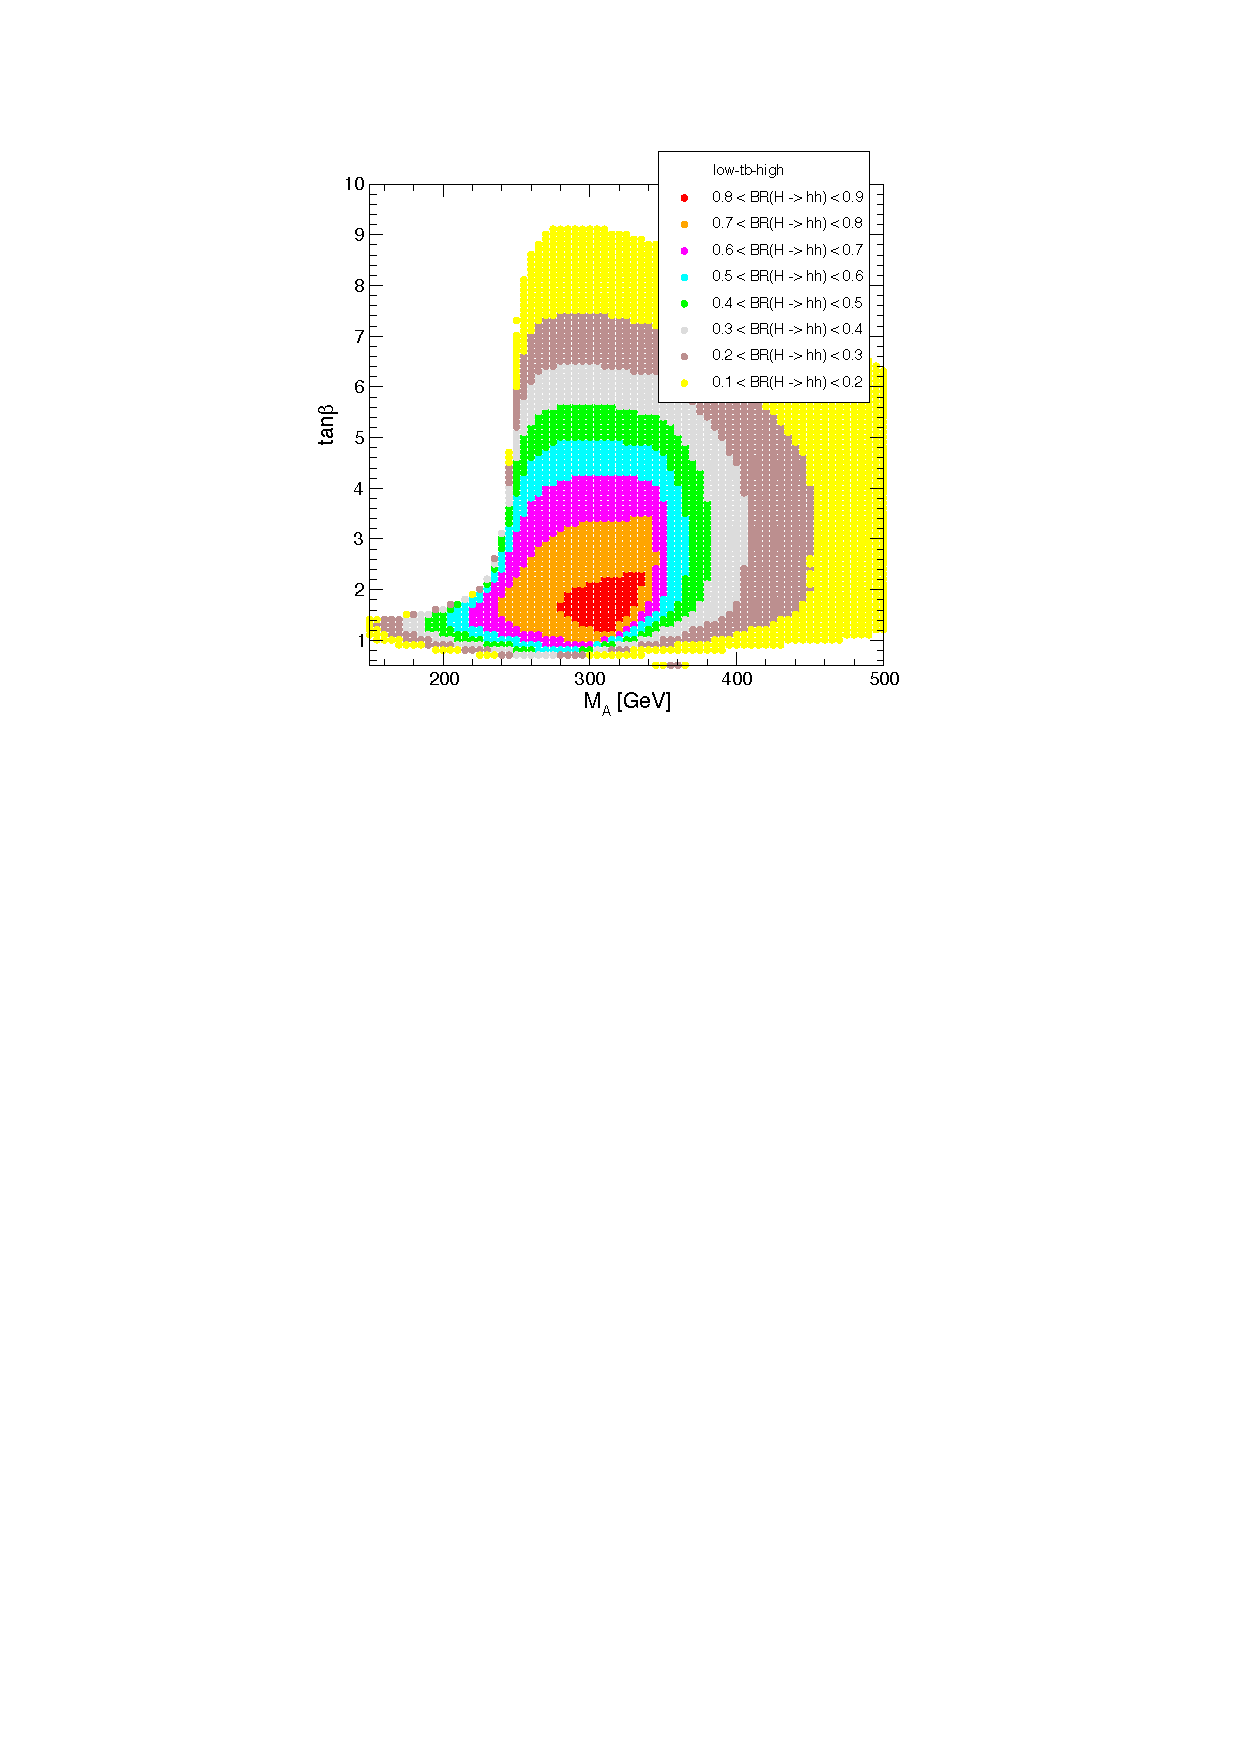
\includegraphics[width=0.5\textwidth]{plots/theory/low-tanb-high-BR.pdf}
\caption[Branching ratios for the $\PH\to\Ph\Ph$ process in the low-$\tan\beta$-high
scenario for different values of $m_{\PA}$ and $\tan\beta$.]{
Branching ratios for the $\PH\to\Ph\Ph$ process in the low-$\tan\beta$-high
scenario for different values of $m_{\PA}$ and $\tan\beta$. The branching ratio
can be significantly enhanced in these regions~\cite{lowtanbhighwiki}.}
\label{fig:lowtanbhighBRs}
\end{figure}


An alternative method for defining such a scenario uses the $m_{\Ph}=125\,\GeV$
mass constraint to define the radiative corrections at each point in the
$m_{\PA}-\tan\beta$ space, such that no particular choices for the \ac{SUSY} breaking
parameters is necessary. This is found to produce similar cross-sections times
branching ratios as the low-$\tan\beta$-high scenario. More detail on this
method can be found in~\cite{Djouadi:2015jea}. Both methods are currently being studied by the 
\ac{LHCHXSWG}~\cite{LHCHiggsCrossSectionWorkingGroup:2011ti,Dittmaier:2012vm,Heinemeyer:2013tqa}. 



 




  \chapter{The CMS experiment}
\label{chap:detector}

\section{The LHC}
\label{sec:theLHC}

The Large Hadron Collider (LHC) \cite{theLHC} is a synchrotron accelerator
with a $27\,\kilo\metre$ circumference designed to
collide beams of protons at centre of mass energies as high as $14\,\TeV$. It is
hosted in the tunnel of the former Large Electron Positron (LEP) \cite{LEP:1983aa} experiment on the French-Swiss border
near Geneva and operated by the European Organisation for Nuclear Research
(CERN). As well as proton-proton collisions, the LHC also accelerates beams of
lead ions to produce both lead-lead (PbPb) and proton-lead (pPb) collisions.

Protons originate from hydrogen gas, the atoms of which are stripped of
their electrons using an electric field. The protons are then accelerated to an
energy of $50\,\MeV$ in the Linac 2 accelerator. Proton bunches are formed inside
the \ac{PSB}, increasing the energy to $1.4\,\GeV$. The \ac{PS} creates proton
beams from the bunches, increasing the energy to $26\,\GeV$. Further acceleration
in the \ac{SPS} raises the beam energy to $450\,\GeV$ before being injected into
the LHC. The LHC contains two beams circulating in opposite directions. The
design operation conditions consist of each beam containing up to 2800 bunches
spaced $25\,\ns$ apart and made up of $\mathcal{O}(10^{11})$ protons each. 
Approximately 1200 superconducting dipole magnets keep the beams circulating
before collisions. The beams collide at four points around the LHC where they
are recorded by four detectors: ALICE \cite{Aamodt:2008zz}, ATLAS
\cite{Aad:2008zzm}, CMS \cite{Chatrchyan:2008aa} and LHCb \cite{Alves:2008zz}. A
schematic of the LHC ring and the detectors is shown in figure
\ref{fig:LHCschematic}.

\begin{figure}[htbp]
   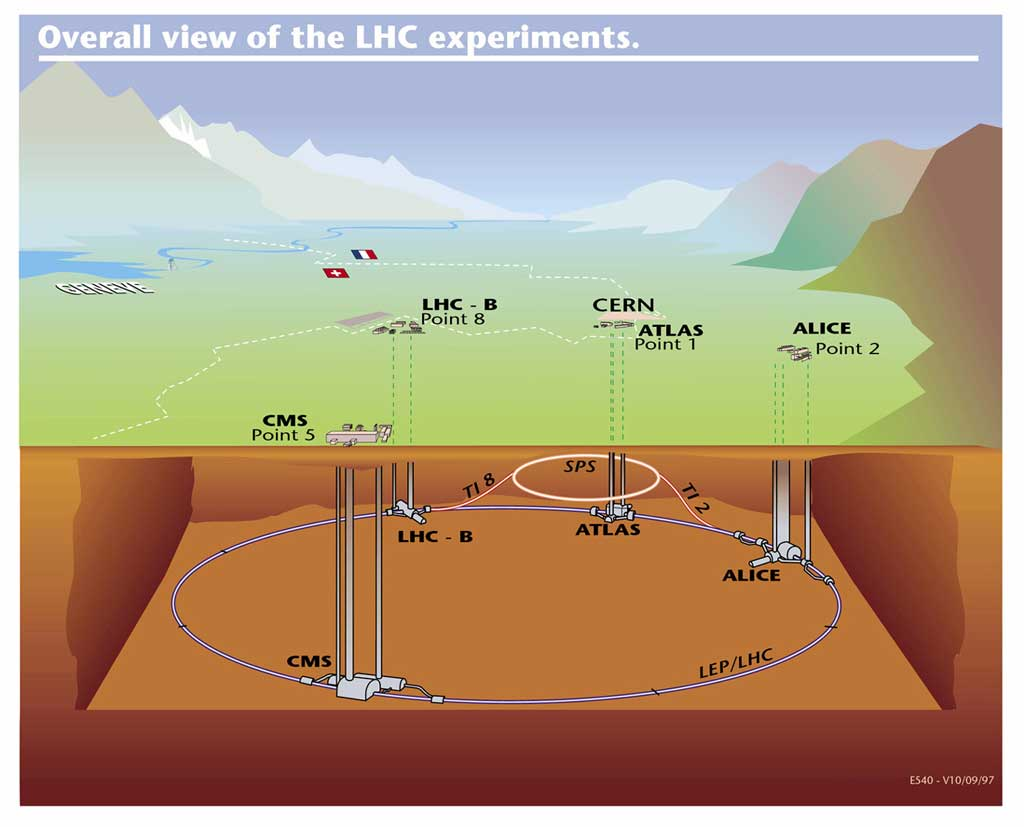
\includegraphics[width=0.7\textwidth]{plots/detector/LHC_layout_sch.jpg}
\caption{Schematic of the LHC accelerator, showing the positions of the four
large detectors.}
\label{fig:LHCschematic}
\end{figure}

The LHC was designed to study physics at the $\TeV$ scale. One of the major
goals of the ATLAS and CMS detectors is to understand the mechanism behind
electroweak symmetry breaking and search for the Higgs boson predicted by this
mechanism in the \ac{SM}. The detectors are also used in searches for \ac{BSM}
physics, with the huge acceleration power of the LHC allowing studies of 
interactions at higher energies than have ever been possible before. 

Higgs boson production occurs only rarely amongst other possible interactions from known
\ac{SM} processes. Figure~\ref{fig:LHCcrosssections} shows the cross-sections of
some of these processes compared with the total proton-proton cross-section. It can be
seen that \ac{SM} Higgs boson production has a cross-section some $10^{-9}$ times
smaller than the total proton-proton cross-section. 
As such, it is necessary to collect large numbers of
collisions to ensure sufficient numbers of events containing these rare
processes. Hence the LHC operates at a high instantaneous luminosity of up to
$10^{34}\,\lumiunits$, where luminosity is defined as:

\begin{equation}
L=\frac{N_{b}^{2}n_{b}f_{\text{rev}}\gamma}{4\pi\epsilon_{n}\beta^{*}}F,
\end{equation}

where $N_{b}$ is the number of protons in the bunch, $n_{b}$ is the number of
bunches, $f_\text{rev}$ is the revolution frequency, $\gamma$ is the Lorentz
factor, $\epsilon_{n}$ is the normalised emittance, $\beta^{*}$ is the beta
function at the collision point and $F$ is a reduction factor due to the
crossing angle.

\begin{figure}[htbp]
   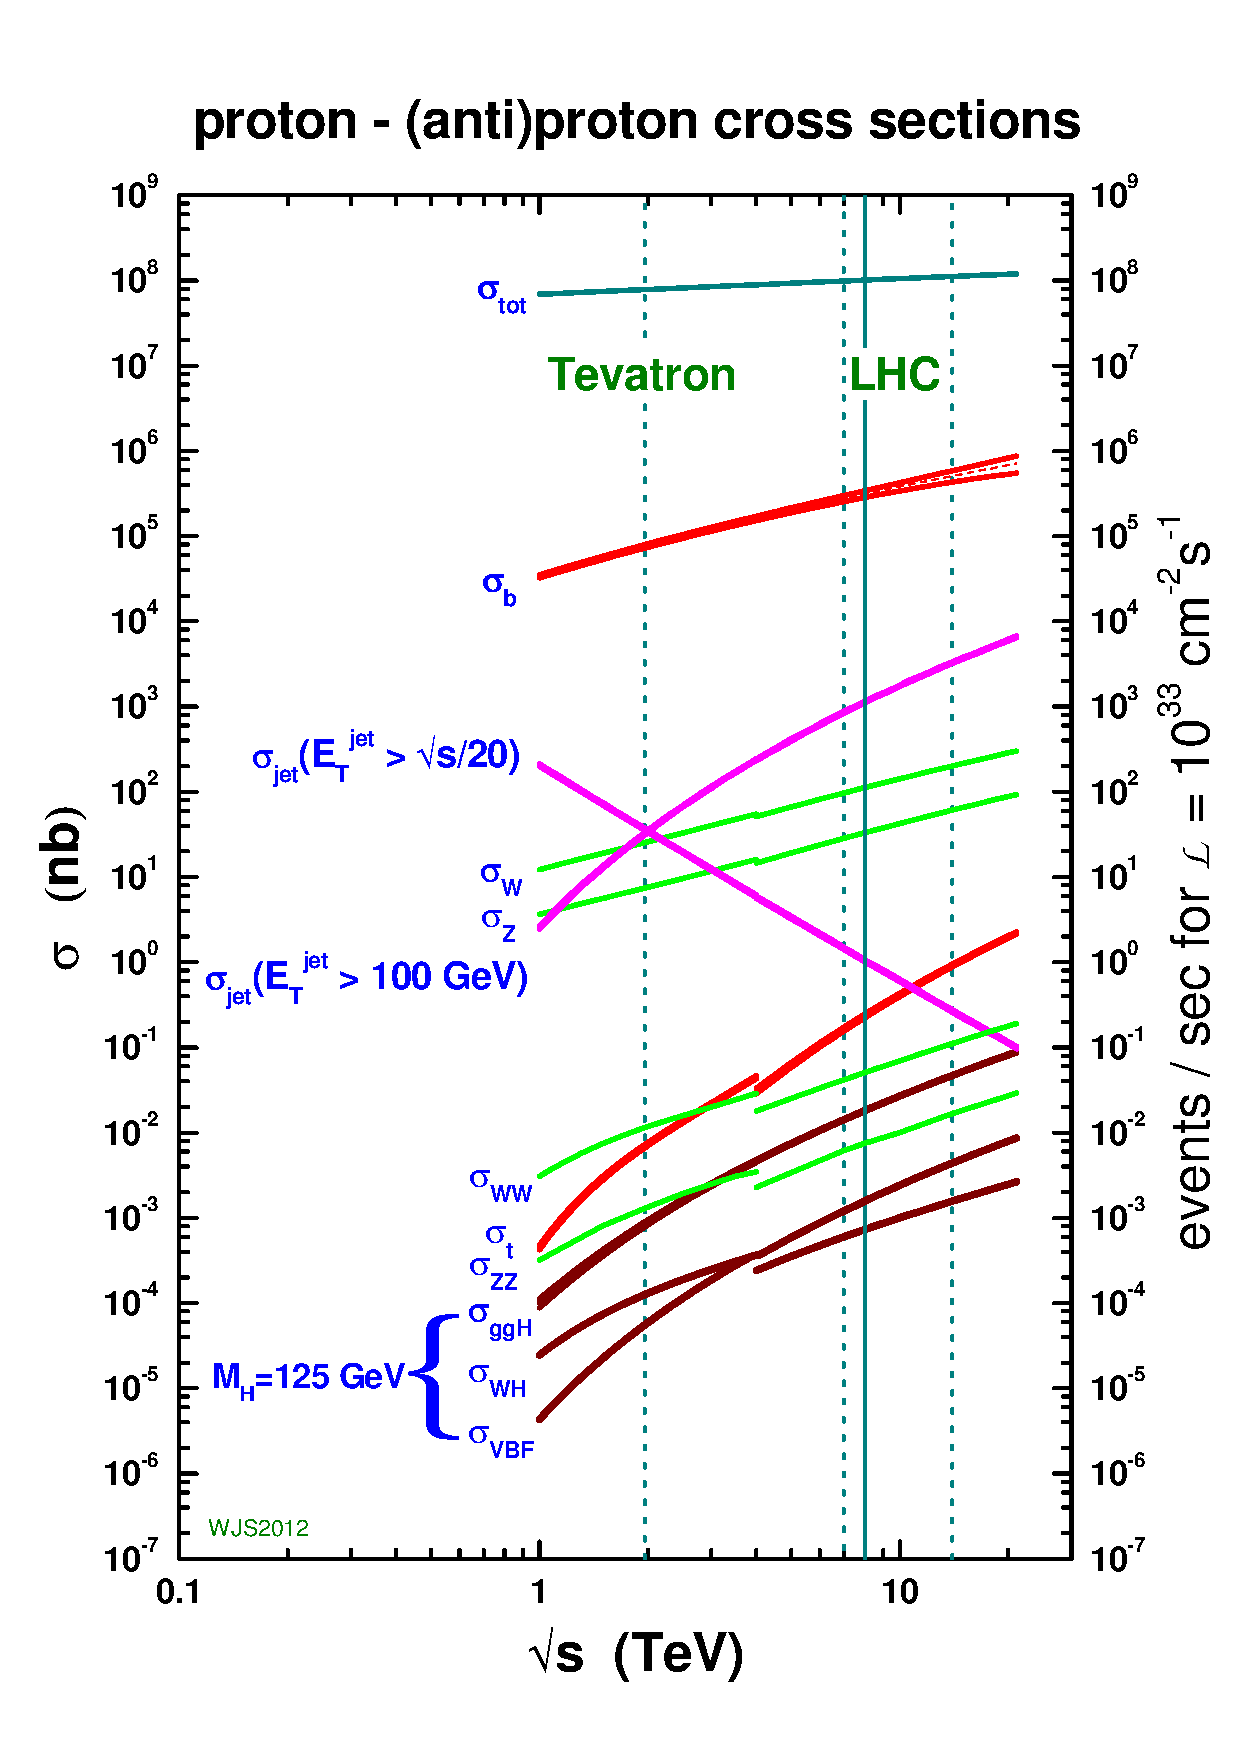
\includegraphics[width=0.6\textwidth]{plots/detector/crosssections2012_v5.pdf}
\caption[Cross sections for several processes in proton-proton or proton-anti
proton collisions, dependent on centre of mass energy.]
{Cross sections for several processes in proton-proton or proton-anti
proton collisions, dependent on centre of mass energy. Energies of the LHC at
different points in running history are highlighted, as is the energy of the
Tevatron. It can be seen that even with the high energies of the LHC, the
cross-section for Higgs boson production is several orders of magnitude smaller than
the total cross-section \cite{stirling:xsecs}.}
\label{fig:LHCcrosssections}
\end{figure}

The LHC began its first major physics run in May 2010 with a centre of mass
energy of $\sqrt{s} = 7\,\TeV$ and gathered an integrated luminosity of $44.2\,\invpb$
before the winter break. It then continued at $\sqrt{s} = 7\,\TeV$
producing an integrated luminosity of $5.6\,\invfb$ in 2011, before increasing to
$\sqrt{s} = 8\,\TeV$ for the 2012 run, where it collected $23.3\,\invfb$,
completing Run 1 of the LHC.
During this time the LHC operated with a bunch spacing of $50\,\ns$. 
Figure~\ref{fig:detlumi} shows the summary of the
integrated luminosity collected by the CMS detector during Run 1 of the LHC,
which concluded in early 2013. Not all luminosity delivered by the LHC is
certified for use in physics analyses - only those events where it is known that
the whole CMS detector was operating successfully, and so the usable luminosity
was reduced to $5.1\,\invfb$ in 2011 and $19.7\,\invfb$ in 2012.
It was after the 2011 run and $\approx6\,\invfb$ of the 2012 run that the
observation of a boson consistent with the Higgs boson of the \ac{SM} was
announced in July 2012 \cite{CMSobservation125,ATLASobservation125}. 

\begin{figure}[htbp]
   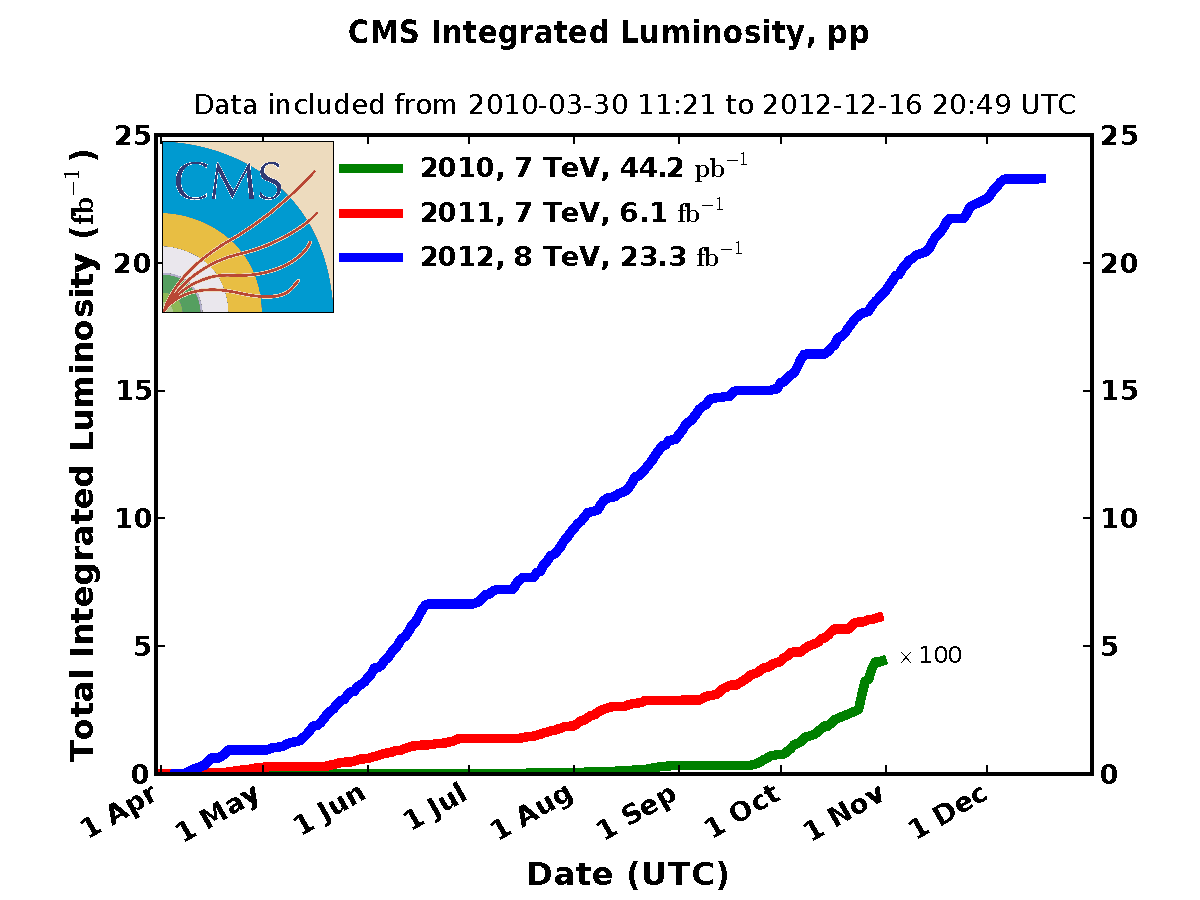
\includegraphics[width=0.7\textwidth]{plots/detector/int_lumi_cumulative_pp_2.pdf}
\caption[Illustration of the total integrated luminosity collected by CMS during
Run 1 of the LHC.]{Illustration of the total integrated luminosity collected by
CMS during Run 1 of the LHC, separated into the 3 years of running \cite{cmslumitwiki}.}
\label{fig:detlumi}
\end{figure}

Since the LHC operates at such high luminosity, the probability of multiple
proton-proton collisions occurring in each bunch crossing is very high. Figure 
\ref{fig:PU} shows the number of interactions per bunch crossing in the
2012 dataset, where the average number was 21. The number for 2011 was slightly
lower at 9 due to the lower instantaneous luminosity. 
These additional collisions on top of the interesting
underlying process in an event are referred to as \ac{PU}.

\begin{figure}[htbp]
   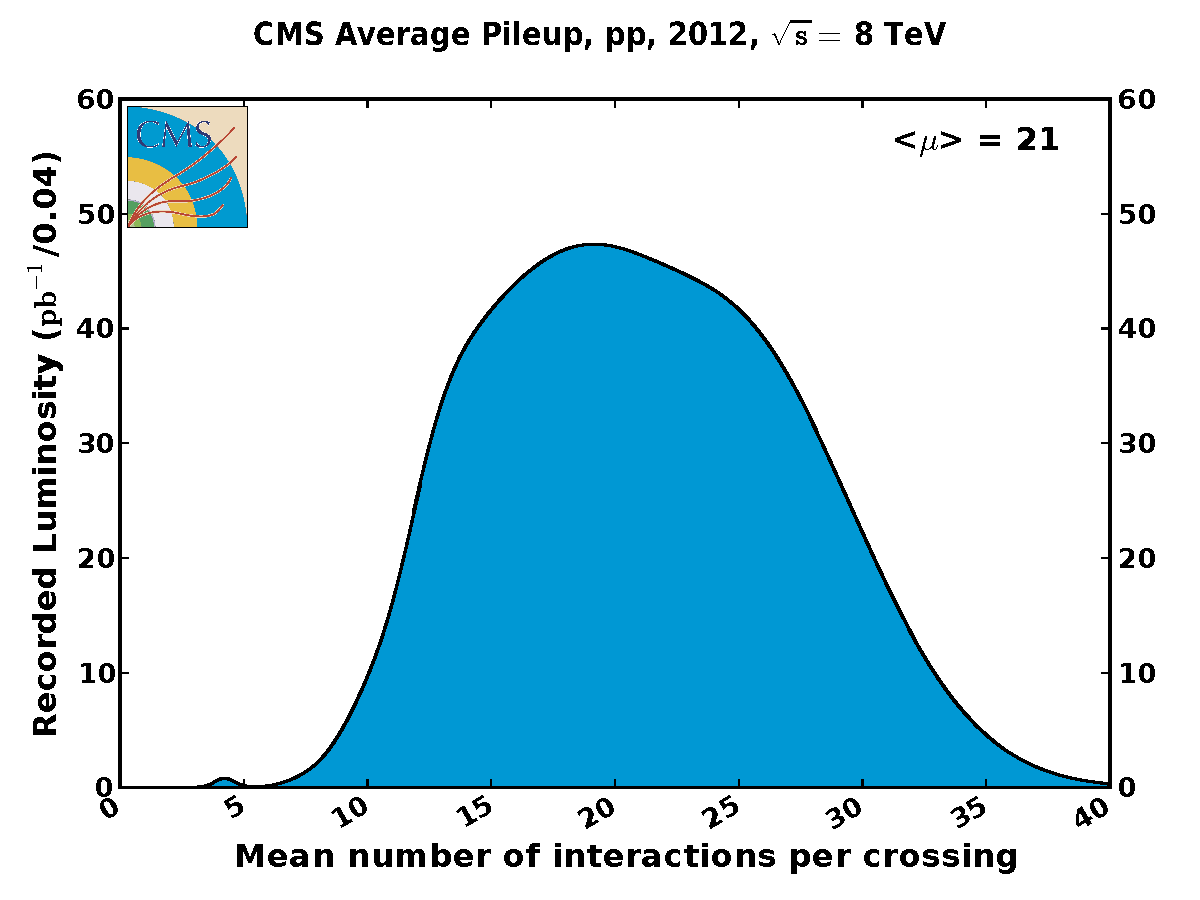
\includegraphics[width=0.7\textwidth]{plots/detector/pileup_pp_2012-2.pdf}
\caption[Distribution of number of pileup events per bunch crossing in 2012
data.]{Distribution of number of pileup events per bunch crossing in 2012 data \cite{cmslumitwiki}.}
\label{fig:PU}
\end{figure}

\section{The CMS experiment}
\label{sec:CMSInDetail}

The CMS detector is a general purpose detector designed to search for the
\ac{SM} Higgs and new physics. As discussed in section~\ref{sec:SMHiggs}, the
mass of the Higgs boson is not directly predicted by the \ac{SM}, and hence upon
design it was important that CMS be able to achieve sensitivity to the \ac{SM} Higgs for a
wide range of possible masses. As shown in figure~\ref{fig:SMHiggsBRs}, at different
Higgs masses the branching ratios of the Higgs boson to different final states
vary considerably, and so CMS must be able to detect the particles from all
possible decay channels. Thus CMS is a hermetic detector featuring
a layered system of different subdetectors, each of importance to the detection
of different particles. 

\begin{figure}[htbp]
   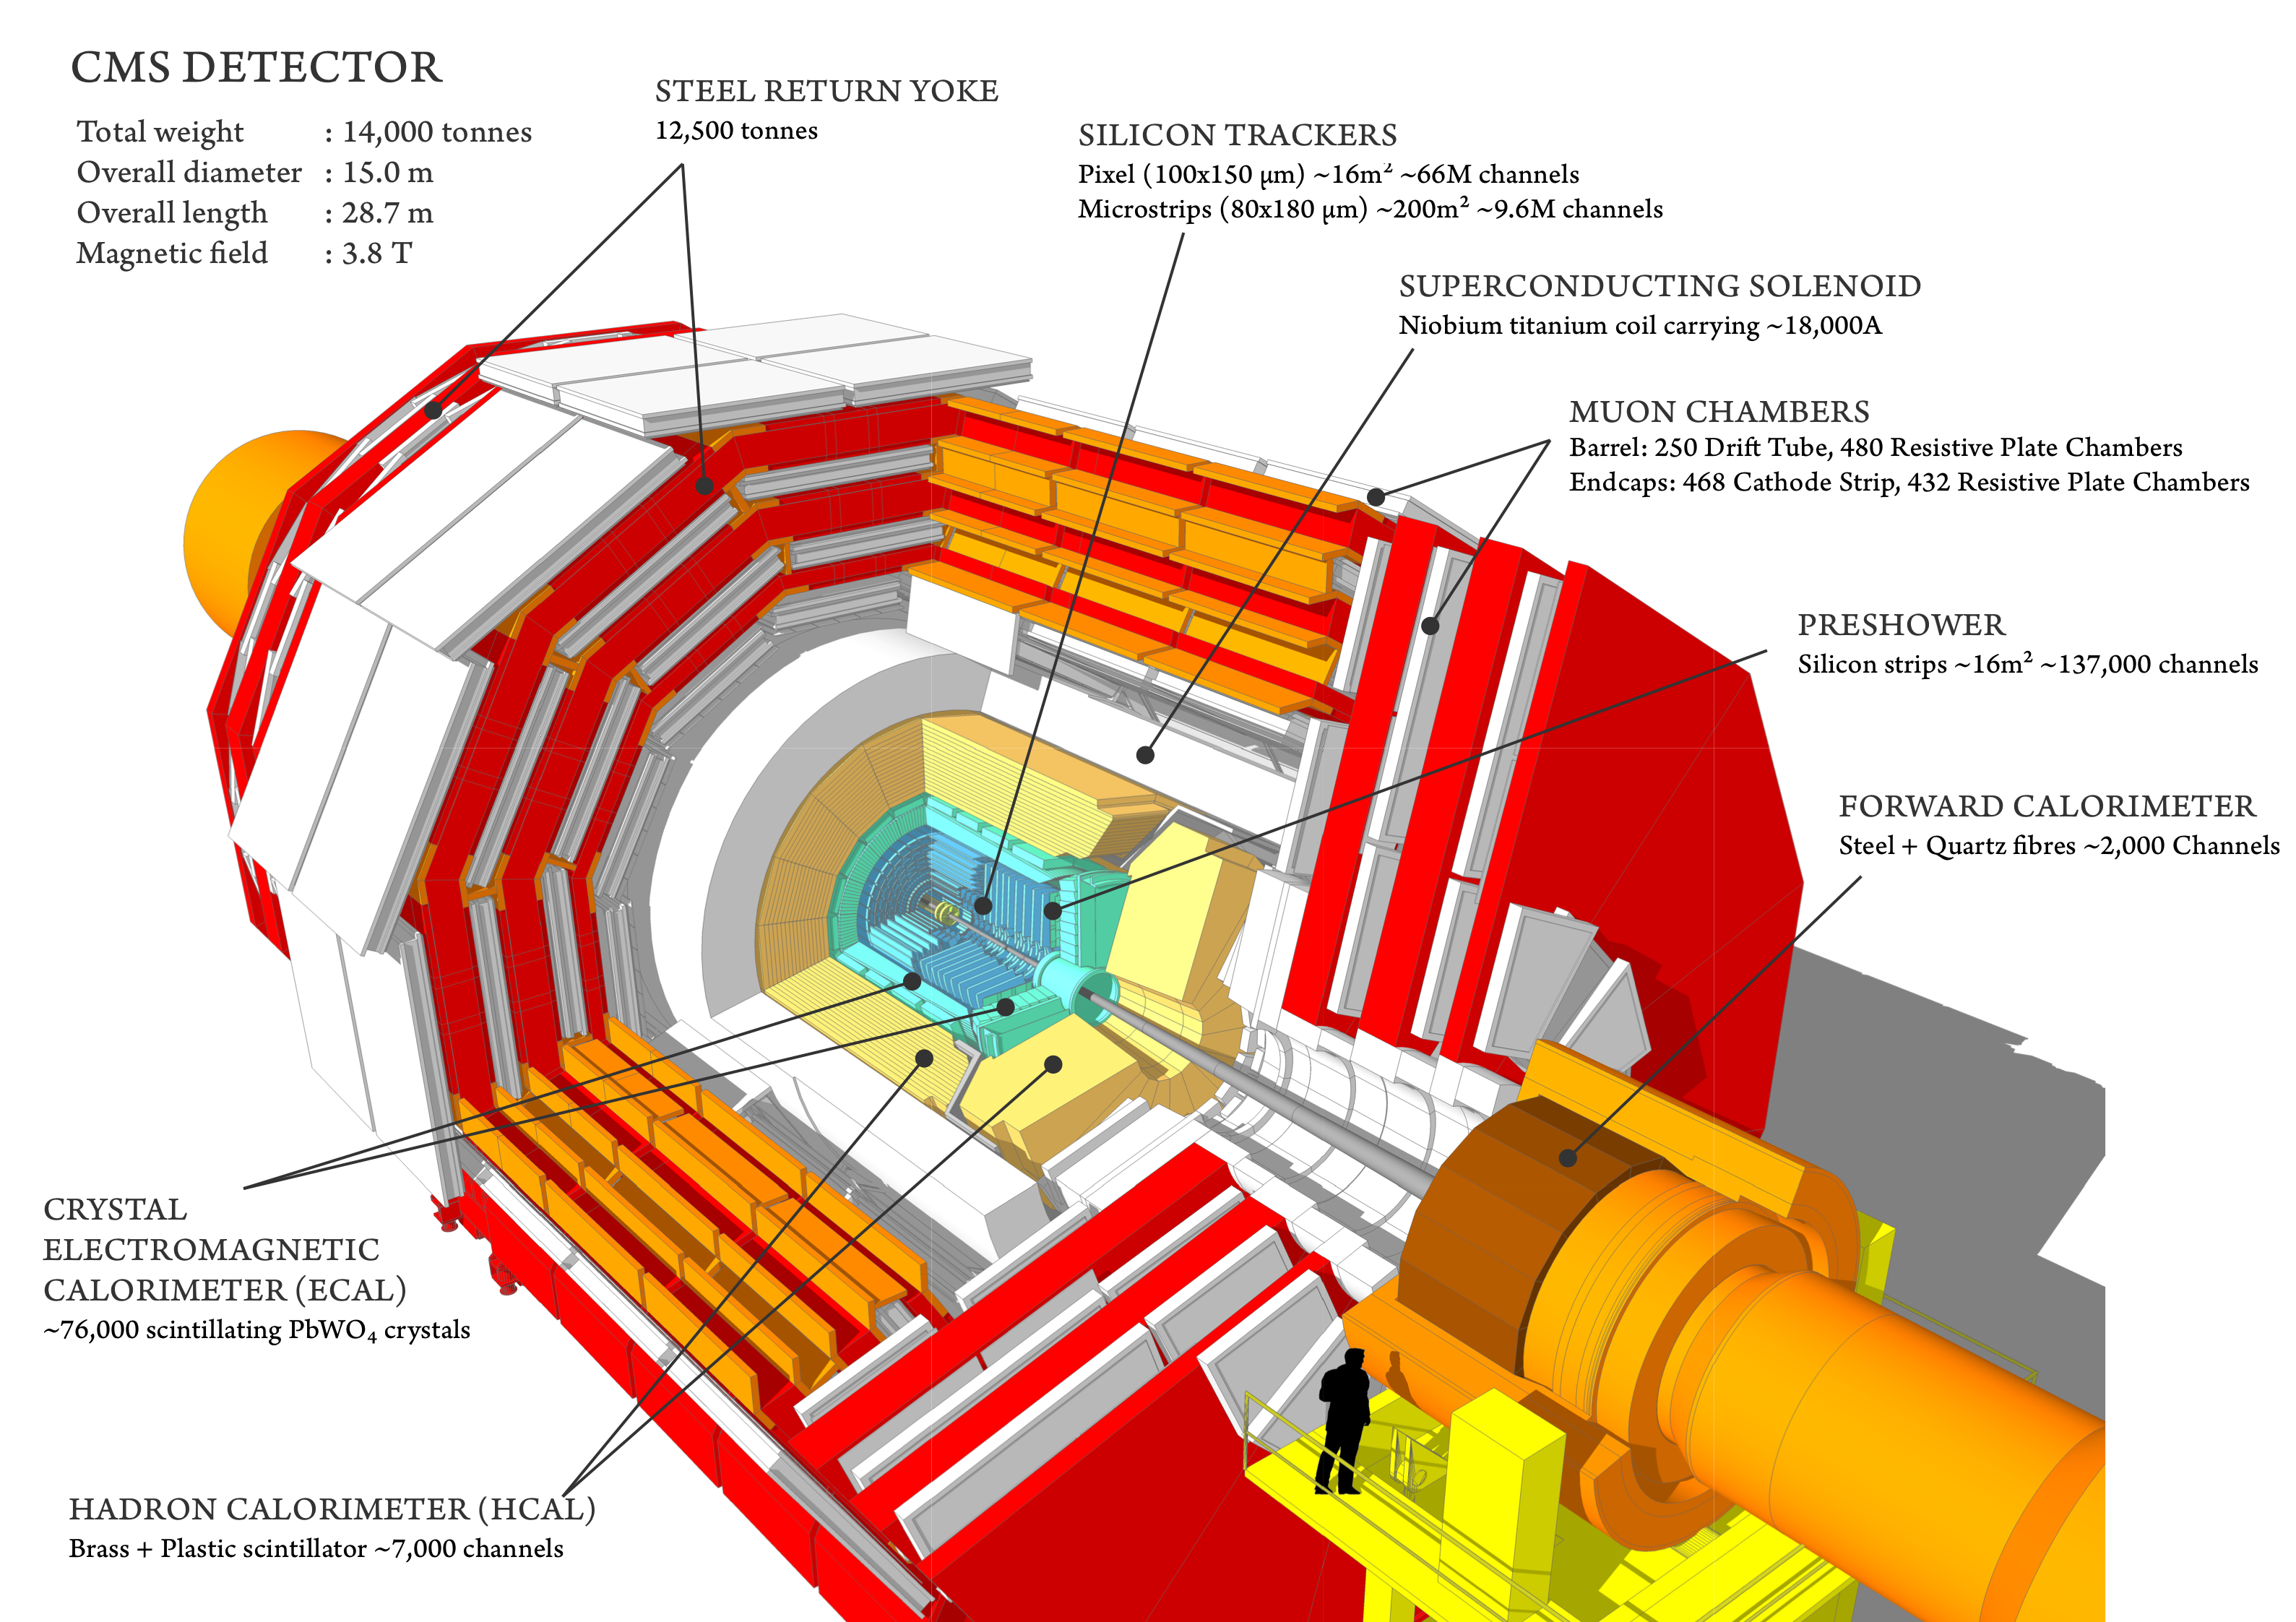
\includegraphics[width=0.95\textwidth]{plots/detector/CMS_Schematic.png}
\caption[A schematic of the CMS detector, illustrating the positions of the
various subdetectors.]
{A schematic of the CMS detector, illustrating the positions and of the
various subdetectors~\cite{1742-6596-513-2-022032}.}
\label{fig:CMSschematic}
\end{figure}

A schematic of the CMS detector is shown in figure~\ref{fig:CMSschematic}. 
The first layer is the tracker, which records the tracks of charged particles,
from which can be extracted the particle's momentum and the location of the
vertex from which it originated. This is followed by the \ac{ECAL} which measures
energy deposited in electromagnetic showers from electrons or photons. The
\ac{HCAL} does a similar job for the hadronic activity, by providing energy
measurements of collections of hadrons, known as jets, which deposit energy
through nuclear interactions. The \ac{HCAL} is a sampling calorimeter, meaning
that the active material is sandwiched between dense absorbing material to
increase the depth of the calorimeter to around 11 radiation lengths. The
\ac{HCAL} coverage is increased in the forward regions by the addition of 
the \ac{HF} calorimeter. The tracker and calorimeters are encased within a 3.8T axial magnetic
field provided by a superconducting magnet which forms the next layer. This
magnetic field provides the mechanism for deflecting the charged particle paths in
a curve such that their momentum can be measured by the size of the curve in the
track and their charge by the direction. The
outermost layers form the muon detector systems, interspersed with iron plates
of the return yoke of the magnet. Muons deposit little energy
through the detector and often travel through to the surrounding cavern. 
%The entire CMS detector is $22\,\metre$ long and $15\,\metre$ in diameter
%\cite{Chatrchyan:2008aa}.

CMS uses a right handed cartesian coordinate system. The
origin is placed at the nominal interaction point with the $z$ axis collinear with the
beam. Then the $x$ axis is chosen to point towards the centre of the LHC ring
and forms a plane with $y$, the remaining transverse coordinate perpendicular to
$x$ and $z$. The angle $\phi$ is the azimuthal angle with respect to the $x$
axis and $\theta$ is the polar angle in the $x$--$y$ plane. Another coordinate
often used is pseudorapidity, defined as:
\begin{equation}
\eta = - \ln[\tan(\theta/2)]. 
\end{equation}

Distance in the $\eta$-$\phi$ plane is given by $\Delta R =
\sqrt{\Delta\phi^{2} + \Delta\eta^{2}}$.
Another important quantity relating to the measurement of collisions is the
projection of the momentum of a particle onto the transverse plane: $\pt =
\sqrt{p_{x}^{2} + p_{y}^{2}}$. The corresponding transverse energy is referred
to as $E_{\text T}$. Hard collisions generally produce particles with
high $\pt$. Descriptions of the detector often separate the regions of
``barrel'' and ``endcaps'', which correspond to the main cylindrical body of
the detector or the circular ends enclosing the cylinder respectively. 

%Figure~\ref{fig:CMSslice} shows a slice of the CMS detector, illustrating 
%the paths of various particles through the different subdetectors.

%\begin{figure}[htbp]
%   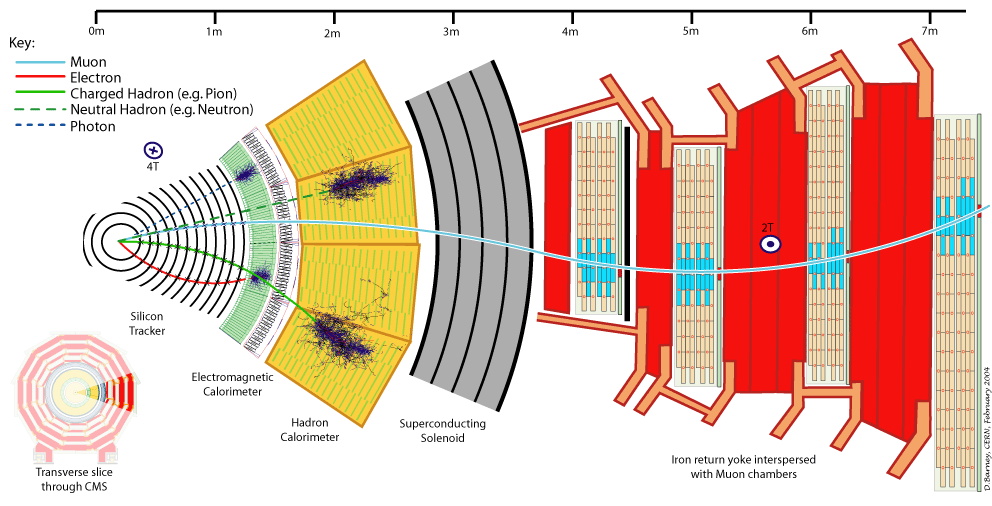
\includegraphics[width=0.9\textwidth]{plots/detector/CMS_Slice.png}
%\caption[A slice of the CMS detector, indicating the various subdetectors.]
%{A slice of the CMS detector, indicating the various subdetectors. The
%paths taken by different types of particles travelling through the detector are
%indicated.}
%\label{fig:CMSslice}
%\end{figure}

\subsection{Tracker}
\label{sec:tracker}

The CMS tracker is designed to reconstruct charged particles close to the
interaction point \cite{Chatrchyan:2008aa}. The magnetic field in combination with the tracker allows
measurement of the particle's momentum and charge. This requires a high level of
granularity to make precise measurements of positions of particles and hence to
locate the vertex from which they originate. Due to the design bunch spacing
of the LHC of $25~\ns$, the rate of collision is extremely high, and so the tracker is
required to be both fast response and radiation hard. This motivates the use of a
silicon based tracking system.

The layout of the tracker is shown in figure~\ref{fig:trackerlayout}.
The tracker is composed of layers of silicon pixel and strip detectors covering
the pseudorapidity range $|\eta| < 2.5$. The pixel detector consists of 66
million individual silicon pixels, each $100~\micron \times 150~\micron$
in size, forming three layers in the barrel region and two in each endcap. The
spatial resolution of the pixel detector is $10$ and $20\micron$ in the $r$--$\phi$ plane
and the $z$ direction respectively, allowing a three-dimensional vertex reconstruction.
Surrounding the pixel detector are layers of strip detectors. These consist of
four cylindrical layers which extend to $r=55\,\cm$ referred to as the
\ac{TIB}, and three disks in each endcap referred to as the \ac{TID}. Each strip
is $10$--$20\,\cm$ long and $80$--$180\,\micron$ wide. Surrounding the \ac{TIB}
and \ac{TID} is the \ac{TOB}, which which extends to $r=116\,\cm$ and
$z=\pm118\,\cm$ and contains six barrel layers. The \ac{TEC} is comprised of nine
disks covering the endcaps. The position resolution of the strip detectors is in
the range $23$--$52\,\micron$ in the $r$--$\phi$ plane and $230$--$530\,\micron$
in the $z$ direction depending on layer. Better resolution in the $r$--$\phi$
plane is required for the measurement of $\pt$.

\begin{figure}[htbp]
   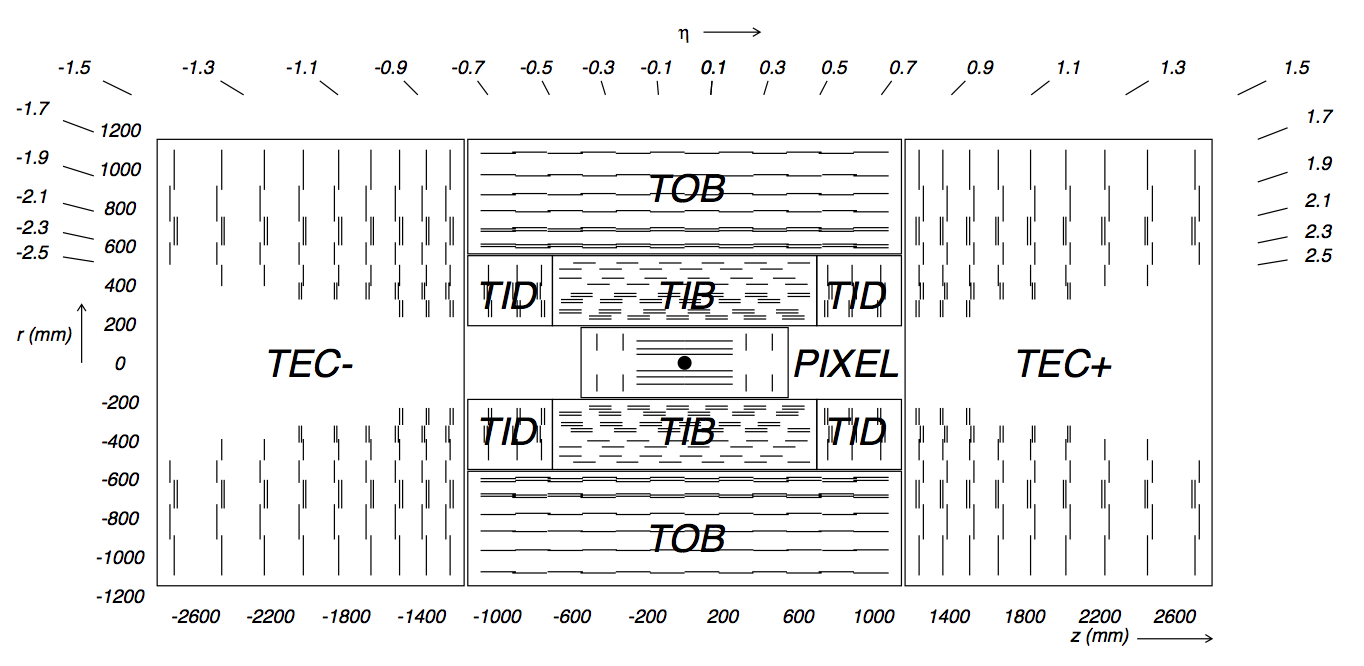
\includegraphics[width=0.9\textwidth]{plots/detector/tracker_layout.png}
\caption[Cross-section of the CMS tracking system, indicating the pixel and
strip detectors and their positions relative to the interaction point.]
{Cross-section of the CMS tracking system, indicating the pixel and
strip detectors and their positions relative to the interaction point \cite{Chatrchyan:2008aa}.}
\label{fig:trackerlayout}
\end{figure}

Tracks are reconstructed using multiple precise measurements throughout the
tracking system. The reconstruction is seeded by triplets of hits in the inner
tracking layers. The trajectory of this seed is extrapolated to the outer tracking
layers using the Kalman filter method \cite{Fruhwirth:1987fm}. The hits found in each layer
which are compatible are added to the trajectory and its uncertainties are
updated until no more compatible hits are found. The use of the tracks to
reconstruct the \ac{PV} is discussed further in section \ref{sec:vertex}.
Momentum resolution degrades with increasing momentum due to decreasing
curvature in the tracks. The $\pt$ resolution of muon tracks is approximately
$1$--$2\%$ for muons with $\pt$ as high as $100\,\GeV$ in the region
$|\eta|<1.6$, rising as high as $8\%$ is the larger $\eta$ regions which have
lower coverage~\cite{Chatrchyan:2008aa}.  

\subsection{Electromagnetic calorimeter}
\label{sec:ecal}

The \ac{ECAL} is constructed from high density lead tungstate
($\mathrm{PbWO_{4}}$) crystals which form a barrel section (EB) 
and two endcaps (EE) outside the tracker~\cite{Chatrchyan:2008aa}. 
$\mathrm{PbWO_{4}}$ was chosen for its
radiation hardness, short radiation length ($0.89\,\cm$) and small Moli\`ere
radius ($2.2\,\cm$), meaning that almost the entire photon or electron energy
can be deposited in the \ac{ECAL}. High energy electrons or photons
entering a crystal initiate an electromagnetic shower, which produces a cascade
of low energy electrons and photons which undergo bremsstrahlung and pair
production respectively. The shower will continue until energy falls below pair
production threshold and ionisation begins to dominate for electrons. 
The depth of each crystal is equivalent to 25.8 radiation lengths, and
thus electrons and photons deposit most of their energy within the crystals.
The atoms in the $\mathrm{PbWO_{4}}$ de-excite by producing scintillation light that is read by
photodetectors. The decay time of the scintillation light is short, such that
about 80\% is emitted before the next bunch crossing (within $25\,\ns$). This
results in a calorimeter with excellent energy resolution, granularity and timing
precision.

Figure \ref{fig:ecal} shows the layout of the \ac{ECAL}. The EB covers the
pseudorapidity range $|\eta|<1.479$. The crystals are arranged in 36 modules such
that the gap between modules are offset by $3^\circ$ with respect to the axis
from the detector origin to avoid particles travelling along the gaps between
crystals. In
the endcaps the crystals are arranged in an $x$--$y$ grid each with an area of
28.6$\,\times\,$28.6 $\mathrm{mm^{2}}$. Two lead plates and two silicon strip
layers mounted before the EE form the pre-shower detectors (PS). These correspond to about
three radiation lengths of absorber material and are designed to initiate
showering and provide sufficient resolution to distinguish single photons from
the pairs produced in neutral pion decays. Uninstrumented regions exist
between the EB and EE, $1.442 < |\eta| < 1.566$, through which cables pass. It
is not possible to provide good measurement of electrons and photons traversing
this region. Overall the \ac{ECAL} covers a pseudorapidity range of $|\eta|<3$.

\begin{figure}[htbp]
   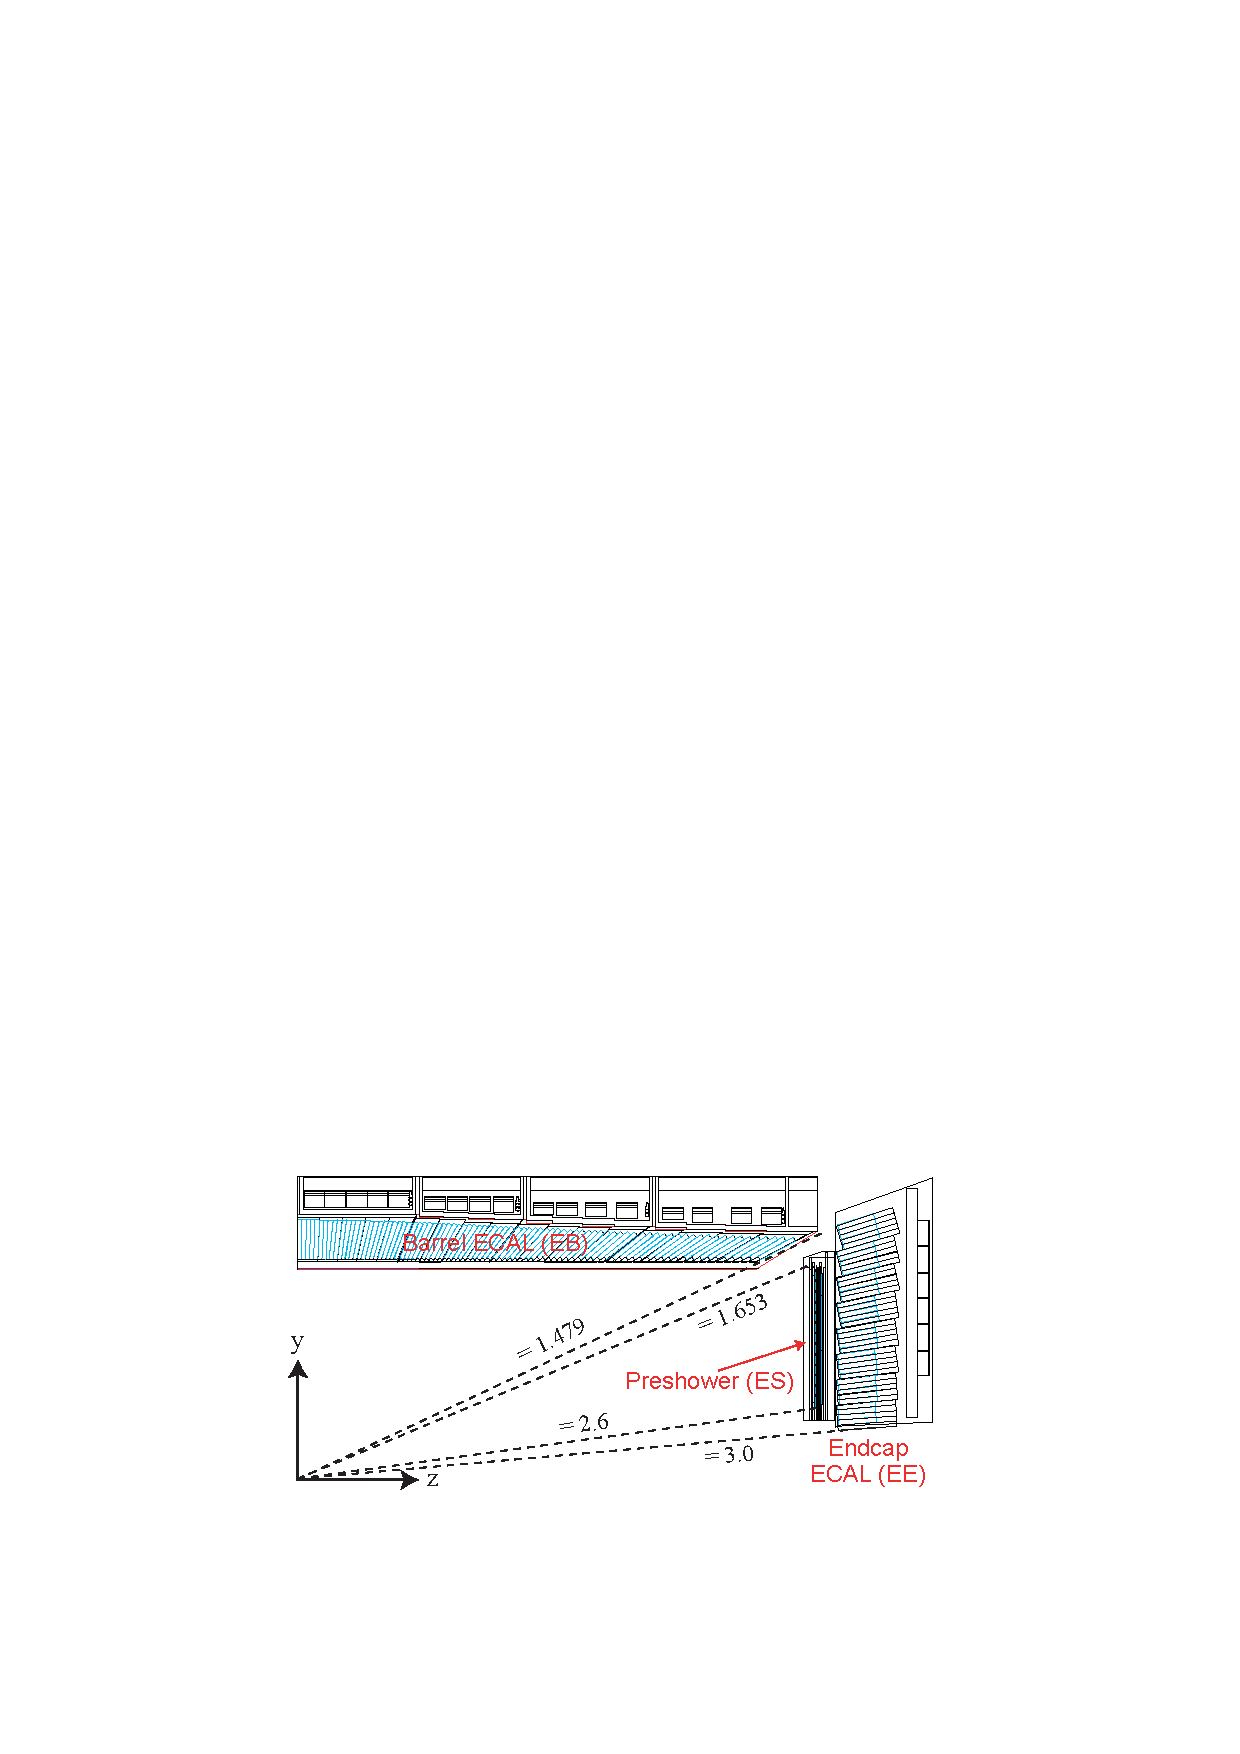
\includegraphics[width=0.9\textwidth]{plots/detector/ecal_layout.pdf}
\caption[Transverse section through the ECAL, indicating its geometry.]
{Transverse section through the \ac{ECAL}, indicating its geometry. The
parts of the detector in the barrel (EB) and endcaps (EE) are indicated
\cite{TDR}.}
\label{fig:ecal}
\end{figure}

The energy resolution of the \ac{ECAL} can be parametrised as a combination of
three unrelated uncertainties as follows:

\begin{equation}
\frac{\sigma}{E} = \frac{A}{\sqrt{E}} \oplus \frac{B}{E} \oplus C , 
\end{equation}

where $E$ is the energy of the incident particle in $\GeV$ and $A$, $B$ and $C$ are the
stochastic, noise and constant contributions respectively. The constants are
derived from test beam data \cite{Chatrchyan:2008aa}. The stochastic term, ($A=2.83\pm0.3\%$),
parametrises stochastic fluctuations in scintillation and shower shape, and is
very low for lead tungstate since the shower can mostly be contained within the
crystals. The noise term $B=0.12~\GeV$ is determined by the electronics. The
constant term $C=0.26\pm0.4\%$ accounts for non uniformity of read-out, 
and limits the \ac{ECAL} accuracy at high energies.
High resolution is essential to allow accurate reconstruction of high energy
photons, such as those produced in $\PH\to\Pphoton\Pphoton$ decays, an important
discovery channel for the \ac{SM} Higgs.

\subsection{Hadronic Calorimeter}
\label{sec:hcal}

The sampling \ac{HCAL} surrounds the \ac{ECAL} and also
covers the pseudorapidity range $|\eta|<3$~\cite{Chatrchyan:2008aa}. The
\ac{HCAL} is designed to detect and measure the energy of strongly interacting
particles. It consists of alternating layers of brass absorber and plastic
scintillator. Brass is used as the absorber material due to its fairly short
nuclear interaction length ($16.42~\cm$) and the fact that it is not magnetic
\cite{PDG}. A hadron shower initiated in an absorber layer causes pulses of 
light in the plastic scintillator tiles which are fed to hybrid photodiodes 
by wavelength shifting fibres. Surrounding the \ac{HCAL} is the solenoid magnet,
which maximises shower containment and reduces non-Gaussian tails in energy
resolution due to energy loss. 

The layout of the \ac{HCAL} is shown in figure \ref{fig:hcal}. The \ac{HB}
covers $|\eta|<1.4$ and is read out in towers of size
$\Delta\eta \times \Delta\phi = 0.087\times0.087$. The \ac{HO}
is a layer of scintillating tiles lining the outside of the solenoid, and
samples the tails of the highly penetrating or late starting showers using the magnet coil as an
absorber. The \ac{HE} at each end of the barrel
consist of towers with dimensions varying between $\Delta\eta \times \Delta\phi
= 0.087\times0.8$ and $0.35\times0.8$. The \ac{HB} provides between 5.8 and 10.6
interaction lengths of absorber, and with combination with the \ac{HO} this increases
to a minimum of $11.8$ interaction lengths. The \ac{HE} provides approximately
10 interaction lengths. 

The \ac{HF} detectors extend the \ac{HCAL} to cover up
to $|\eta|=5.2$ and experience the highest fluxes of particles in the whole
detector, and so are made using radiation hard quartz fibres as the active medium
embedded in a steel absorber. In the \ac{HF} a signal is generated when charged
showering hadrons emit Cherenkov radiation in the fibre, which is detected by
photomultiplier tubes. The \ac{HCAL} contains no
uninstrumented regions. The large coverage of the
\ac{HCAL} is necessary to be able to accurately calculate the missing transverse energy
(\MET) in an event as a result of neutrinos which are invisible to the detector,
using energy balance with the visible objects. This is discussed further in
section~\ref{sec:met}.


\begin{figure}[htbp]
   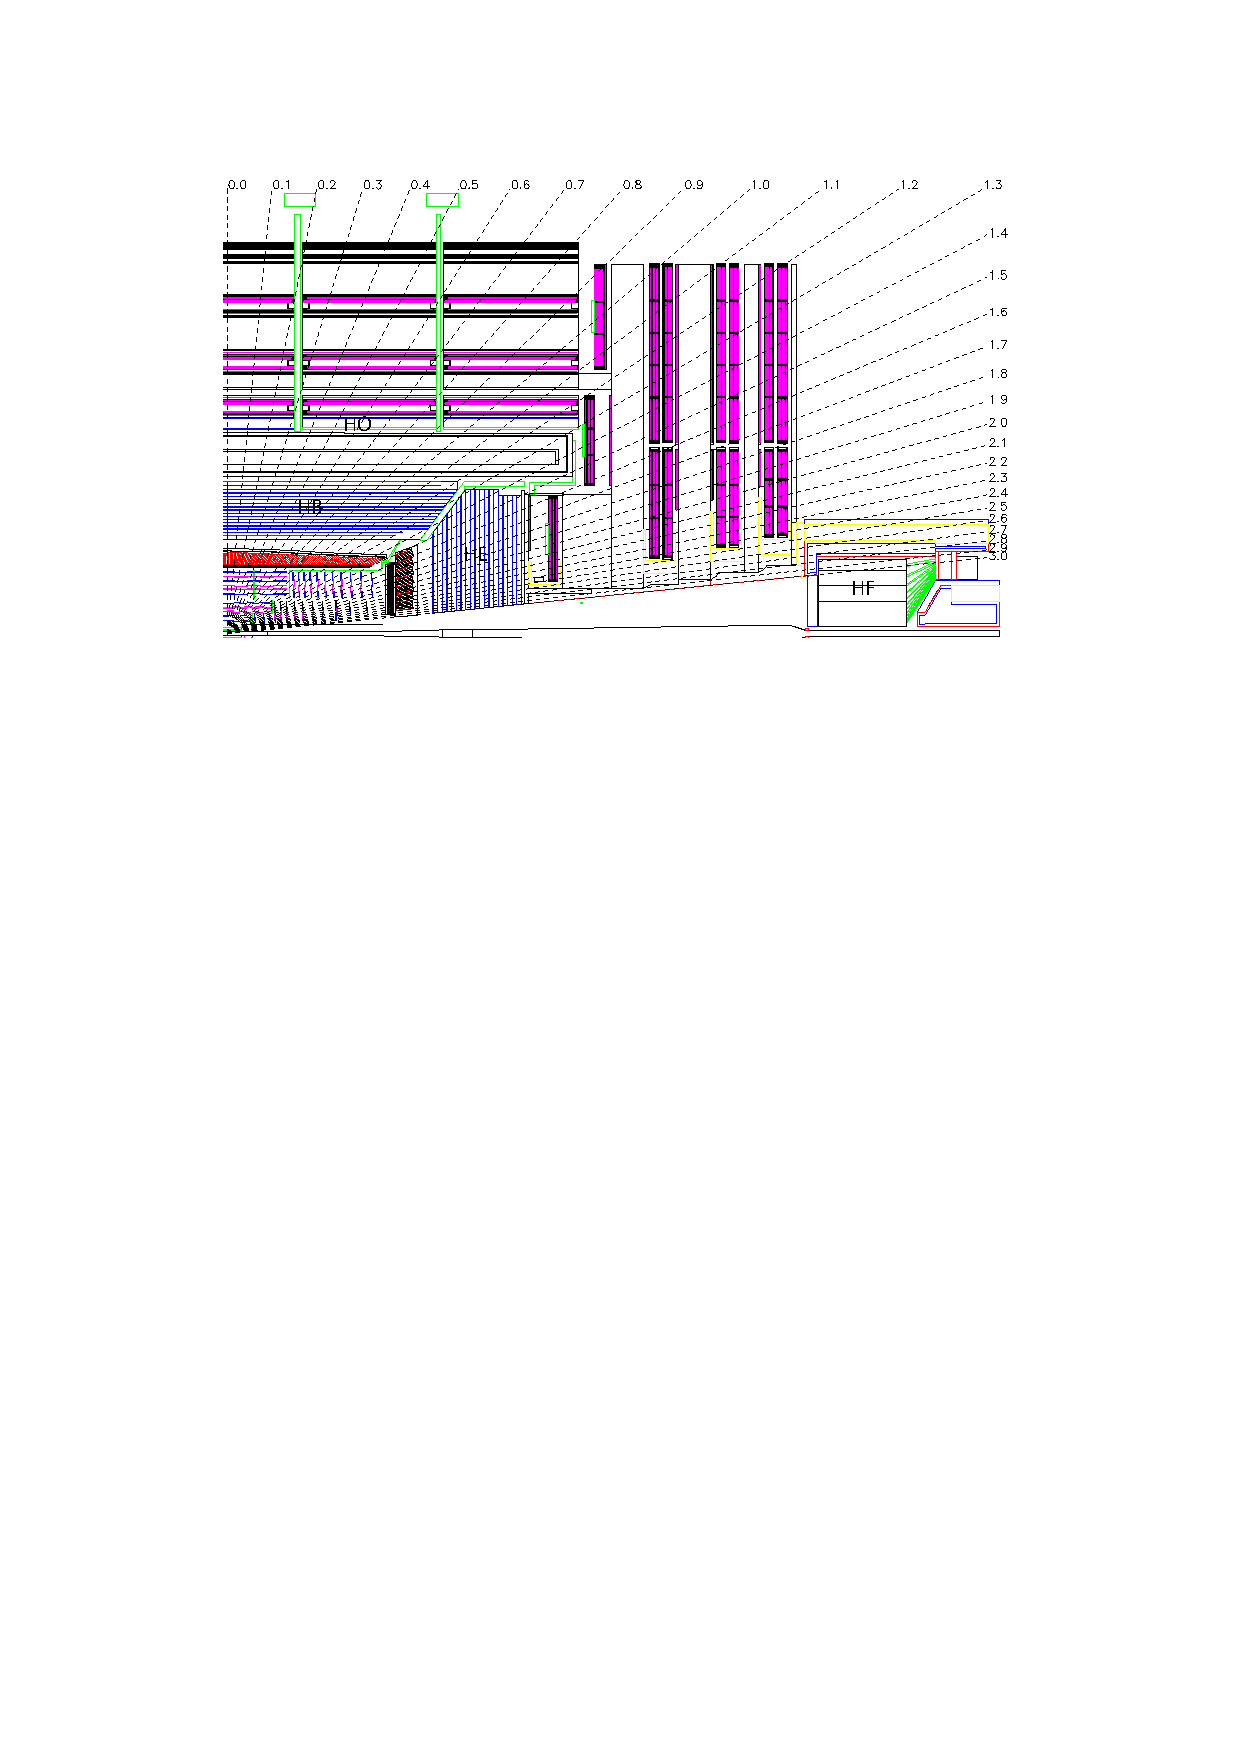
\includegraphics[width=0.9\textwidth]{plots/detector/hcal_layout.pdf}
\caption[Illustration of the HCAL in the r--z plane, indicating its
geometry.]
{Illustration of the \ac{HCAL} in the r--z plane, indicating its geometry \cite{Chatrchyan:2008aa}.}
\label{fig:hcal}
\end{figure}

Both the granularity and the energy resolution of the \ac{HCAL} are worse than
the \ac{ECAL}. The resolution is measured using a test beam of charged pions and
found to be \cite{Abdullin:2009zz}:

\begin{equation}
\frac{\sigma}{E} = \frac{94.3\%}{\sqrt{E}} \oplus 8.4\%,
\end{equation}

where $E$ is the energy of the showering particle. 

\subsection{Muon Detector}
\label{sec:muondetector}

The iron return flux of the magnet is instrumented with the muon detectors
\cite{Chatrchyan:2008aa}, covering a pseudorapidity range of $|\eta|<2.4$. Due
to the fact that muons have considerably higher masses than electrons, they lose
little energy via bremsstrahlung or ionisation, and so typically pass through
the calorimeters and the solenoid without depositing much energy. The muon
systems are therefore used for efficient identification of muons, as well as
being able to provide a complementary measurement of their momentum additional
to the one made in the tracker. The best momentum resolution is achieved by 
combining hits in the tracker and the muon chambers, as described in section~\ref{sec:muons}. 

The muon detector is shown in figure \ref{fig:muondetectors}. The barrel region
(covering $|\eta|<1.2$) consists of the \ac{DT} chambers arranged in four
cylindrical layers positioned between the plates of the magnet return yoke. The
\ac{DT}s are augmented by \ac{RPC} in the range covering $|\eta|<1.6$. The
\ac{DT} chambers consist of a tube of cross-section $13\times42\,\text{mm}^{2}$,
each filled with wires about $2.4\,\metre$ long. The tubes are filled with a
mixture of argon and carbon dioxide gas. When a muon travels through the tube,
it ionises the gas, and free electrons drift towards the anode wire resulting in
an electrical signal. Each chamber consists of several layers of tubes, oriented
in different directions to measure the muon $\phi$ direction and the $z$
coordinate. The position resolution of the \ac{DT}s is approximately
$200~\micron$.

\begin{figure}[htbp]
   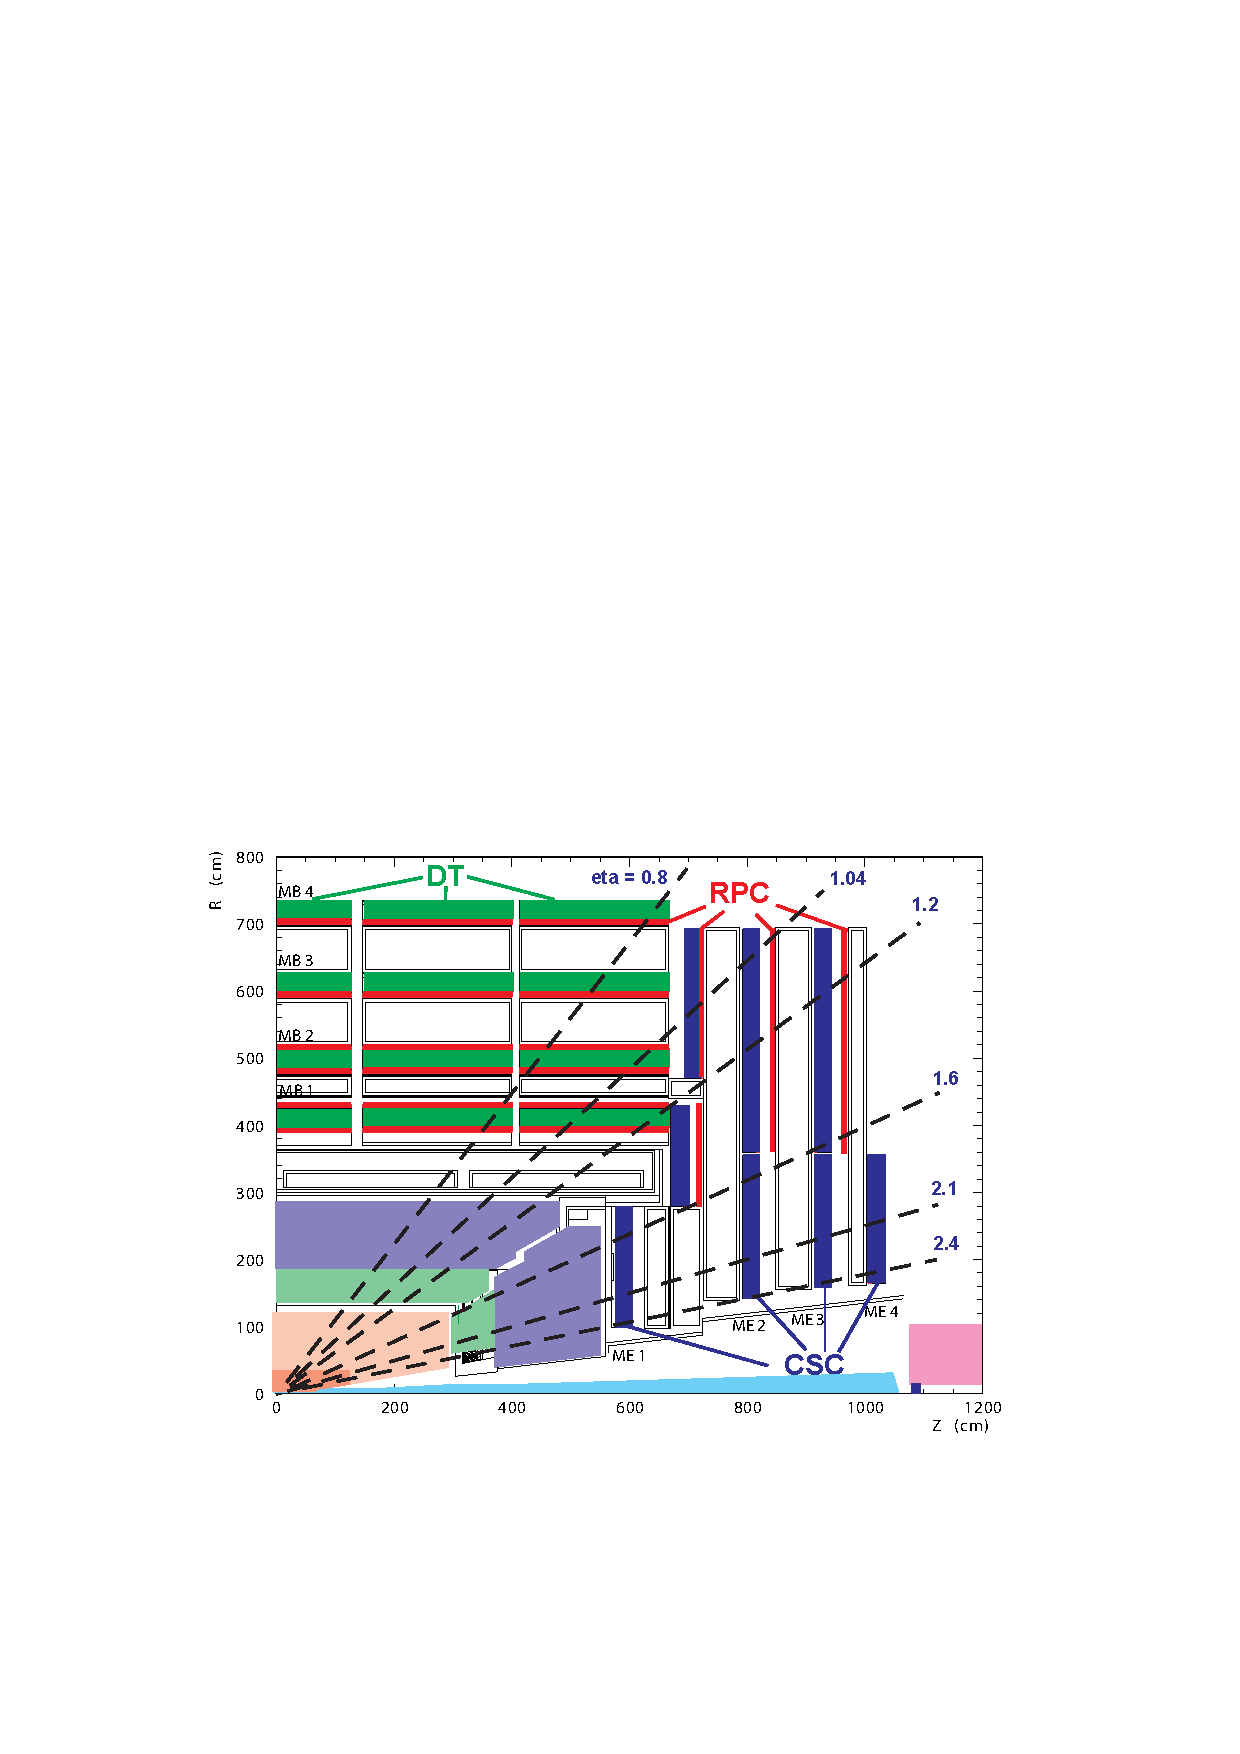
\includegraphics[width=0.9\textwidth]{plots/detector/muon_layout.pdf}
\caption[Layout of one quadrant of the muon systems.]{
    Layout of one quadrant of the muon systems, indicating the positions
of the DT, CSC and RPC \cite{TDR}.}
\label{fig:muondetectors}
\end{figure}

The endcaps use \acs{CSC}, which have a fast response, fine segmentation and are
radiation hard. This is necessary in the endcaps due to the higher rate of muons
and backgrounds. Each \ac{CSC} has six gas layers with cathode strips running
radially outward to measure hits in the $r$-$\phi$ plane, with anode wires
running perpendicular to the cathodes to measure $\eta$. The position resolution
of the \ac{CSC}s varies between 100 and $200~\micron$ depending on $\eta$. In the region
$|\eta|<1.6$, the \ac{CSC}s are augmented by \ac{RPC}s, as in the barrel. The
\ac{RPC}s consist of a gas gap enclosed by parallel anode and cathode plates, in
which the muon ionisation is detected by arrays of metallic strips running
parallel to the beam axis. The \ac{RPC}s have worse resolution than the \ac{DT}s
and \ac{CSC}s but an extremely fast time response of
$1~\ns$, meaning they can be used to correctly identify the bunch crossing in
which a muon originates, and can be used as a dedicated muon trigger.


\subsection{Triggering and data processing}
\label{sec:trigger}

At the design specification of the LHC, the proton bunch crossing rate is
$40~\MHz$, and to date collisions have been recorded at $20~\MHz$, which will
increase to the design $40~\MHz$ in Run 2 starting this year. Each event
consists of approximately $1~\text{MB}$ of data and it is not feasible to write
data at this rate to tape, nor is it feasible for the \ac{DAQ} system to perform
read-out of the events at this rate. Thus the rate at which events are saved is
reduced to $\mathcal{O}(100\,\Hz)$ using a trigger system to select the
interesting events.

The first stage of the trigger system is the \ac{L1} trigger, which is
constructed using custom electronics to incorporate information from the
calorimeters and muon systems only~\cite{Chatrchyan:2008aa}. The \ac{L1} starts with local information
such as calorimeter energy deposits and hit patterns in the muon chambers. A
regional trigger combines this local trigger information from different sections
of the detector to give a $\pt$ sorted list of candidate objects. Finally the
global trigger issues a decision to accept or reject the event based on the
\ac{L1} information from all parts of the detector. This decision is made within
$3.2\,\micro\second$ and hence uses only the front-end electronics. The \ac{L1}
trigger reduces the rate to around $100\,\kHz$.  

Events accepted by the \ac{L1} trigger are then read out to the \ac{HLT}. This
operates on a processor farm of several thousand CPU cores and processes the 
complete detector information, including input from the tracker. The \ac{HLT}
is capable of determining the object momenta with much greater accuracy, and
apply tighter identification criteria, using algorithms much closer to those
used in offline reconstruction. Due to the fact that the instantaneous luminosity
increased across the Run 1 period, the trigger $\pt$ and energy thresholds were
changed several times in order to retain a stable rate of read-out. Over the Run
1 period, CMS operated at a rate of about $1\,\kHz$, with $300\,\Hz$ being promptly
reconstructed and the rest being ``parked'' to be reconstructed after the LHC running
finished when more computing power was freed \cite{CMS:2012ooa}.

Even incorporating the trigger, the rate of production of data by CMS is at
several petabytes per year. The CMS and the other LHC experiments make use of
the \ac{WLCG} \cite{web:grid}, a global data storage and analysis network which
integrates the computing facilities of universities and research institutes
around the world. The system consists of different tiers: the Tier~0 centre at
CERN performs full event reconstruction, before all data are distributed to at
least one Tier~1 centre, to keep a copy at several sites across the globe. A
larger number of Tier~2 centres process this data for specific analyses to give
access to researchers across the globe. 

  \chapter{Event Reconstruction}
\label{chap:reco}

This chapter describes the reconstruction of events collected by the CMS
detector. The $\PH \to \Pgt\Pgt$ analysis uses almost every object measured in
CMS and makes use of information from every sub-detector. 
Section \ref{sec:vertex} describes the reconstruction of the
primary vertex using measured tracks in the event. Sections \ref{sec:electrons}
and \ref{sec:muons} describe the reconstruction of the electrons and muons in
the event combining the tracks with information from the \ac{ECAL} and muon
chambers respectively. Section \ref{sec:jets} describes the reconstruction and
treatment of jets, followed by section \ref{sec:met} describing how the missing
energy of the event is computed. The reconstruction of hadronic taus
is described in section \ref{sec:taus}.

In addition to the reconstruction of the objects used in the $\PH \to \Pgt\Pgt$
analysis, the final section of this chapter contains a description of a tool of
great importance to this analysis - a likelihood based reconstruction of the
di-tau pair mass, described in section \ref{sec:svfit}.

\section{Primary Vertex Reconstruction}
\label{sec:vertex}
%Consider adding track reconstruction here too.

The reconstruction of the \ac{PV} of the event allows us to identify the hard
$pp$ interaction over the other vertices from multiple $pp$ collisions in the same
bunch crossing, known as \ac{PU}. At CMS there was an average of 9
\ac{PU} vertices per event in 2011 data and 21 in 2012. Correct
identification of the \ac{PV} also allows us to distinguish ''prompt" production of
particles, i.e. production at the \ac{PV} from the hard interaction, from
in-flight decays of hadrons or photon conversions.  

The vertices are reconstructed using the tracks in the inner
tracker. A clustering algorithm, called the \ac{DA} algorithm
\cite{DetAnnealing}, is used to assign tracks to their most likely 
vertex. Each vertex is seeded by at least two tracks separated in $z$ by less than
$1~\cm$ at the point of closest approach to the $z$ axis.
The most likely position of each vertex is then determined using the
adaptive vertex fitter \cite{adaptivevertex}. In
this fitter each track is assigned a weight, $w_{i}$, which is close to 1 for tracks which
are highly compatible with the fitted vertex position and close to 0 for tracks with low
compatibility. These weights are used to define the number of degrees of freedom
for the fit as: $n_{dof}^{vertex} = 2\sum_{i}^{\text{tracks}}w_{i}-3$. This
variable is an assessment of the mutual compatibility of the component tracks of
the vertex, and is used to distinguish real $pp$ interactions from
mis-reconstructed vertices. For most analyses, quality cuts \cite{CMS-PAS-TRK-10-005} on each vertex are
applied as follows:
\begin{itemize}
\item The distance in the $z$ direction from the vertex to the nominal interaction
point must be smaller than $24~\cm$. 
\item The corresponding distance in the transverse plane must be smaller than
$2~\cm$.
\item $n_{dof}^{vertex} > 4$.
\end{itemize}

The \ac{PV} is taken to be the vertex with the highest sum squared $\pt$ of its
associated tracks. 

\section{Electrons}
\label{sec:electrons}

Electrons are reconstructed by matching \ac{ECAL} deposits with tracks from the
inner tracker. This is made more difficult by the fact that the electrons
undergo bremsstrahlung when interacting with the material of the tracker.
The photons produced can also convert to $\Pep\Pem$ pairs before
reaching the \ac{ECAL}. This means that the energy deposited in the \ac{ECAL} 
can be spread out in the $\phi$ direction. Hence dedicated algorithms are used
to combine the energy deposits from both the initial electron and the
bremsstrahlung products, known as ``supercluster'' algorithms \cite{ElectronReco}.

The algorithms used are different for electrons in the barrel and endcaps, in
order to be optimal for the different geometries. In both cases, a clustering is performed
in the $\eta-\phi$ plane starting from the \ac{ECAL} crystal with the most energetic deposit, and
continuing outwards to the surrounding crystals until there are no more
unclustered crystals above a certain energy threshold. In the barrel, the
``hybrid'' clustering algorithm is used. In this algorithm the seed crystal has
$\Et > 1~\GeV$ and the clustering is performed in a ``domino'' of $3\times1$ or
$5\times1$ crystals, with additional dominoes (which attempt to collect
radiation deposits) stepping in both $\phi$
directions around the seed up to $\Delta\phi\approx0.3$. The energy threshold
below which crystals are not clustered  is $100~\MeV$. In the endcaps the
approach is similar with a clustering algorithm
is the ``Multi5$\times$5'' algorithm using $5\times5$ arrays of crystals within
$\Delta\eta<0.07$ and $\Delta\phi<0.3$.

The energy-weighted average position of the supercluster is computed, and this
position is the equivalent of the impact point in the \ac{ECAL} of a
non-radiating electron with energy equal to the supercluster energy. This is
matched to a compatible hit in a loose $\phi$-$z$ search region 
in the in the first pixel layer, under the
hypothesis that the electron could be either charge. If a compatible hit is
found, the hit in the first layer is used to update the estimated electron
trajectory which would result in hits in the outer layers. This seeds the
reconstruction of the electron trajectory through the Silicon Strip Tracker
using the \ac{GSF} algorithm \cite{GSFalgorithm}. This provides an additional momentum measurement
which is used to improve the electron energy resolution. 

%Backgrounds to electrons are expected to originate
%in hadronic jets, for example where a $\Pgpz$ and $\Pgppm$ overlap, or where a
%$\Pgppm$ showers early in the \ac{ECAL}.
% read the paper and understand better what these backgrounds are!! pions?
Electron ID criteria are used in many analyses to improve the efficiency of
selecting real electrons over backgrounds which tend to originate from
hadronic jets. The most commonly used variables are \cite{Baffioni:2006cd}:

\begin{itemize}
\item $\Delta\eta_{\text in}$ and $\Delta\phi_{\text in}$, the separation in the
$\eta$ and $\phi$ between the supercluster and track direction
evaluated at the \ac{PV} position and extrapolated to the \ac{ECAL} (generally
smaller for prompt electrons).
\item $\sigma_{i\eta i\eta}$, the energy-weighted $\eta$ width of the cluster.
This is typically small for prompt electrons, which have a more localised
cluster.
\item $H/E$, the ratio of hadronic to electromagnetic energy in the region of
the seed cluster. This is also generally lower for prompt electrons.
\end{itemize}

Figure \ref{fig:electronID} shows the distributions of these variables in both simulated
electrons and jets in the barrel, and the discrimination power can be seen.

\begin{figure}
\begin{center}
\subfloat[]{
    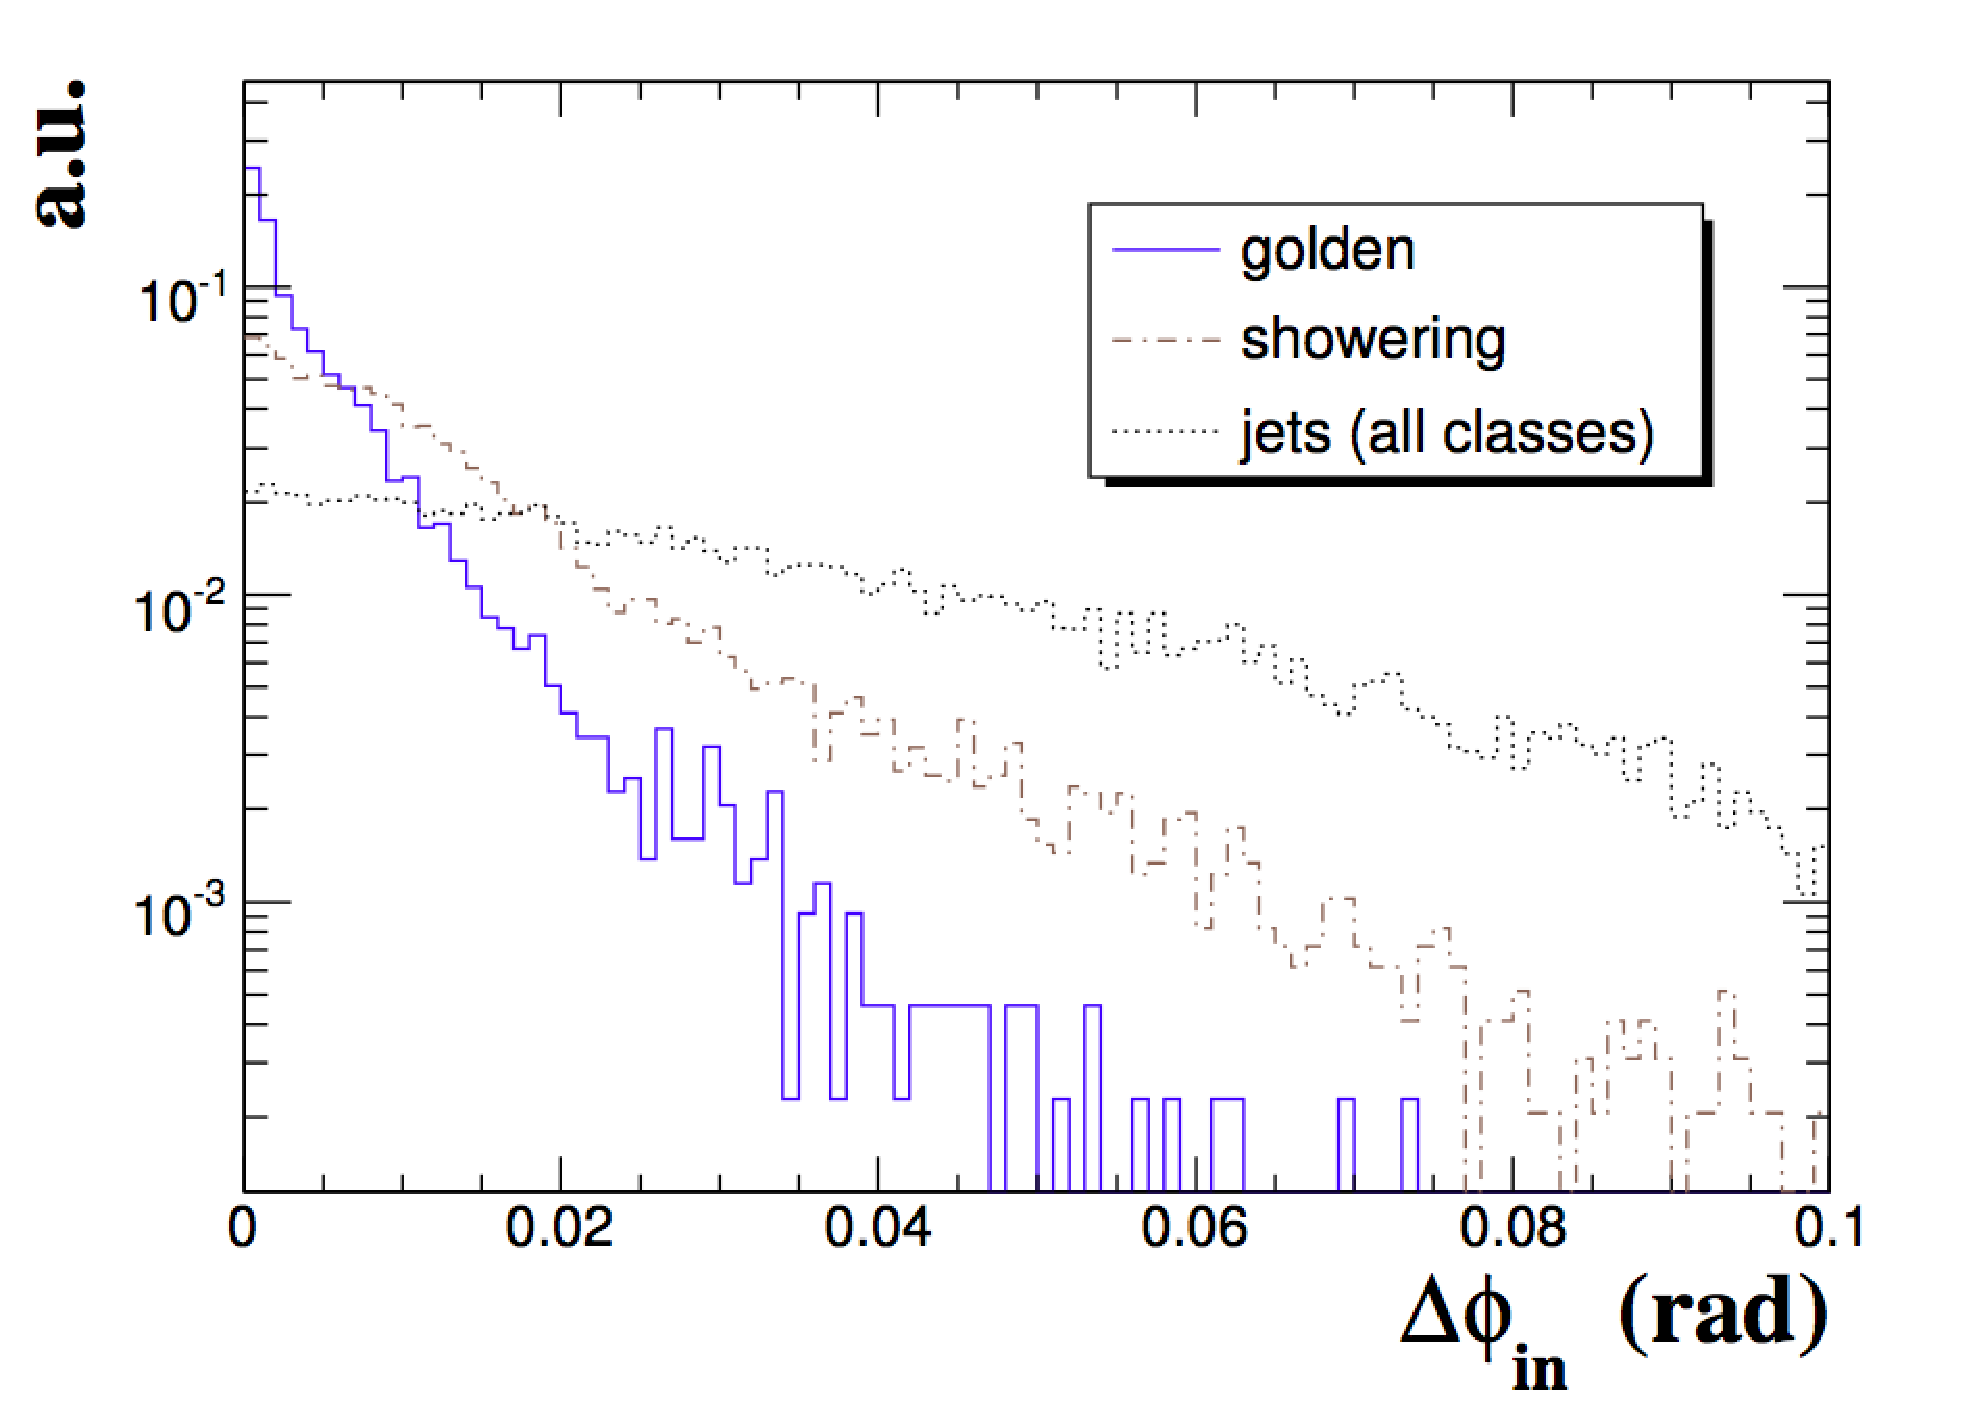
\includegraphics[width=0.5\textwidth]
      {plots/reco/elec-dphi.pdf}}
\subfloat[]{
    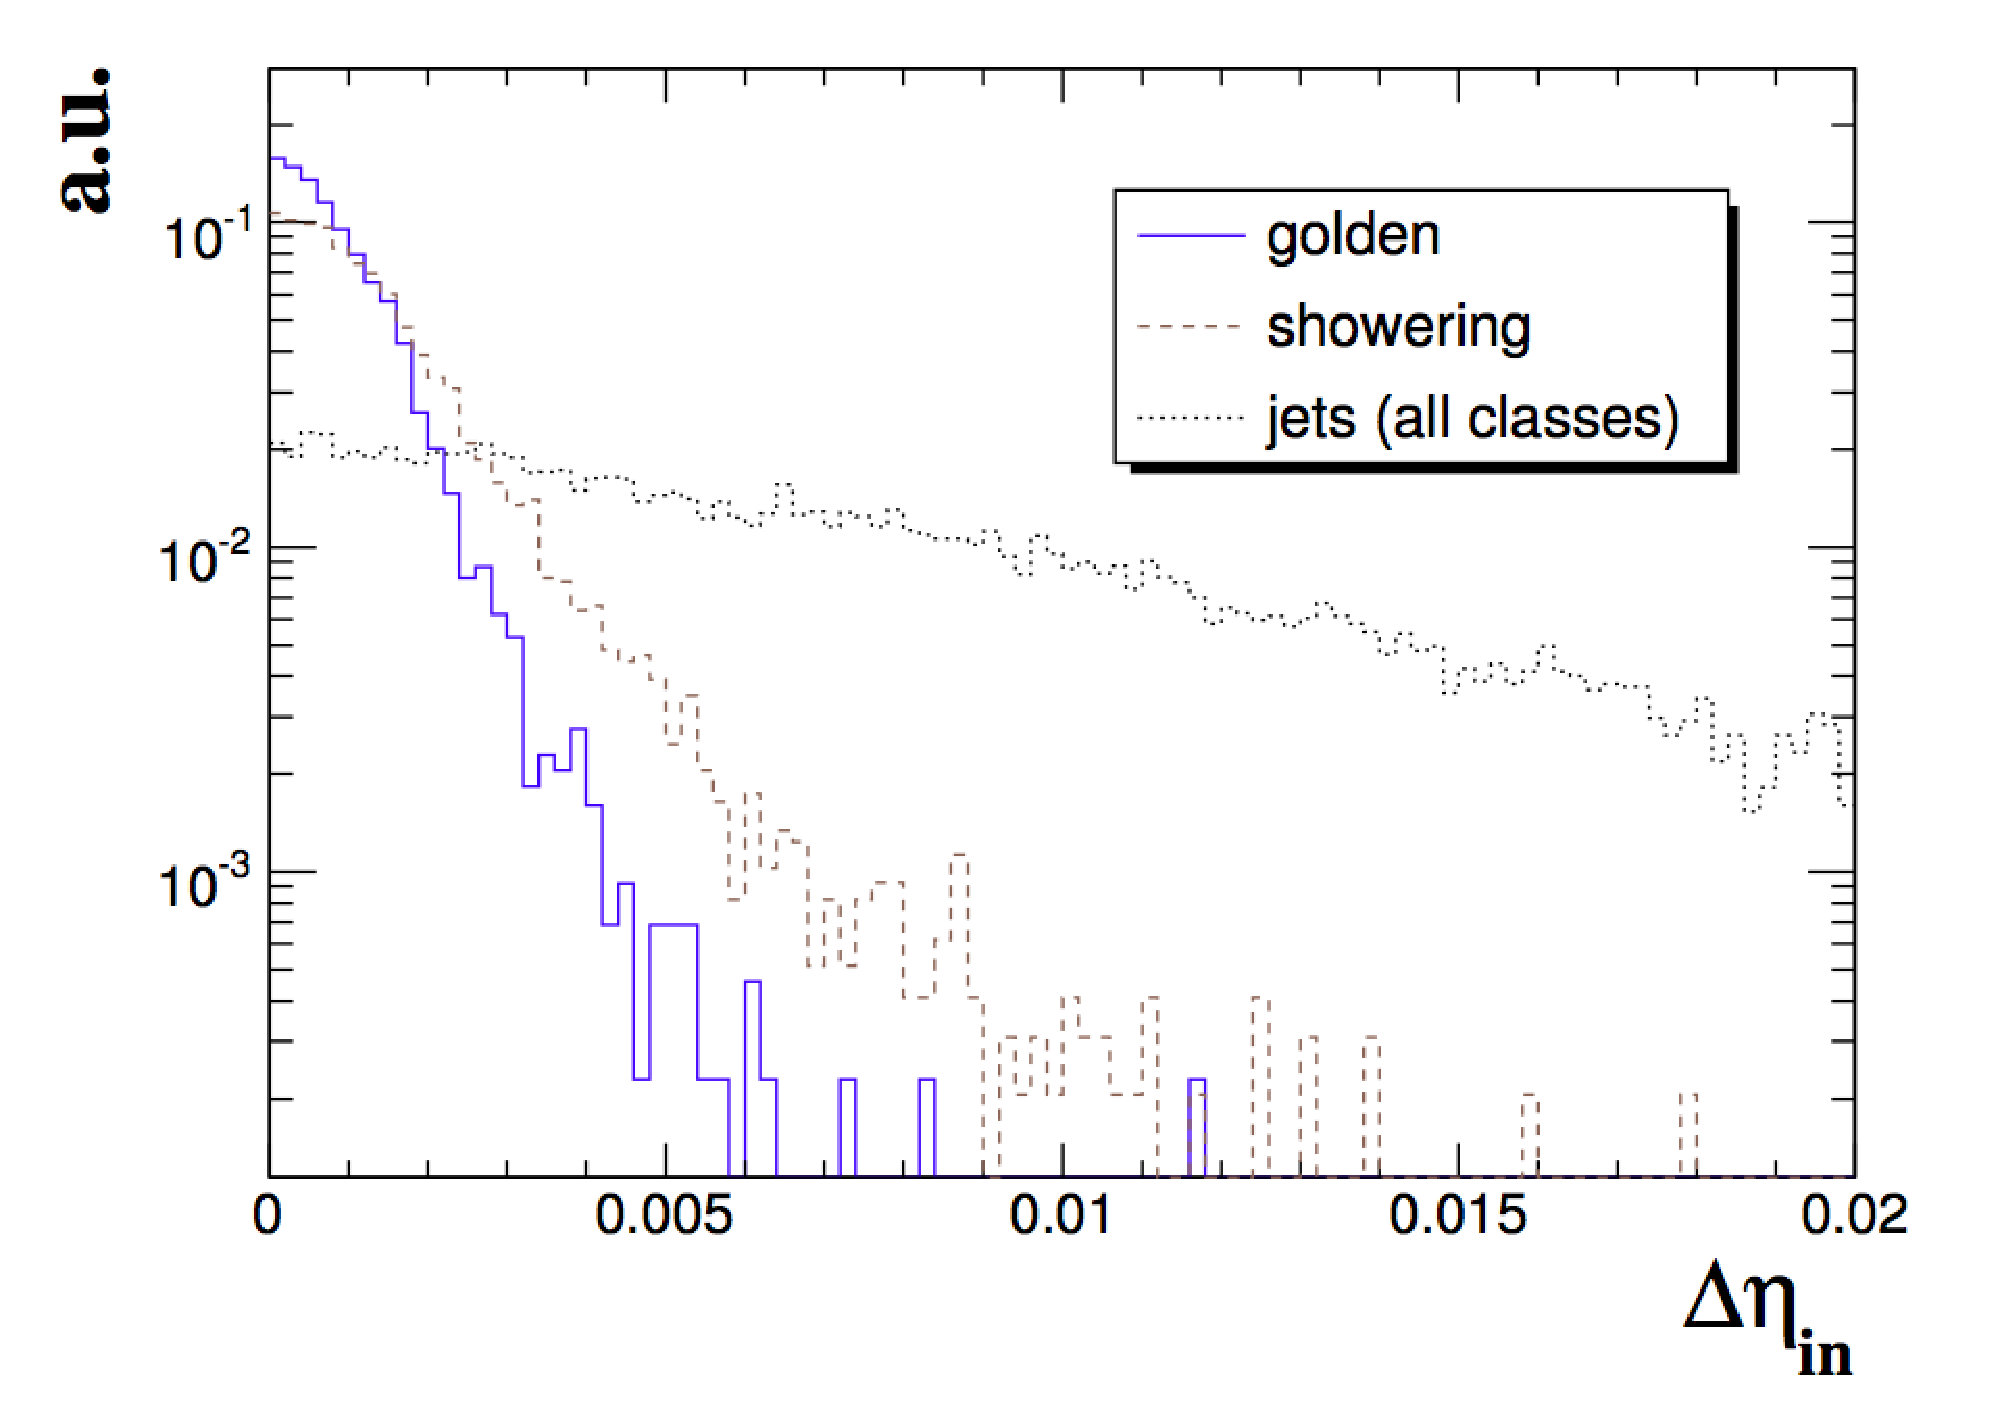
\includegraphics[width=0.5\textwidth] 
      {plots/reco/elec-deta.pdf}} 

\subfloat[]{
    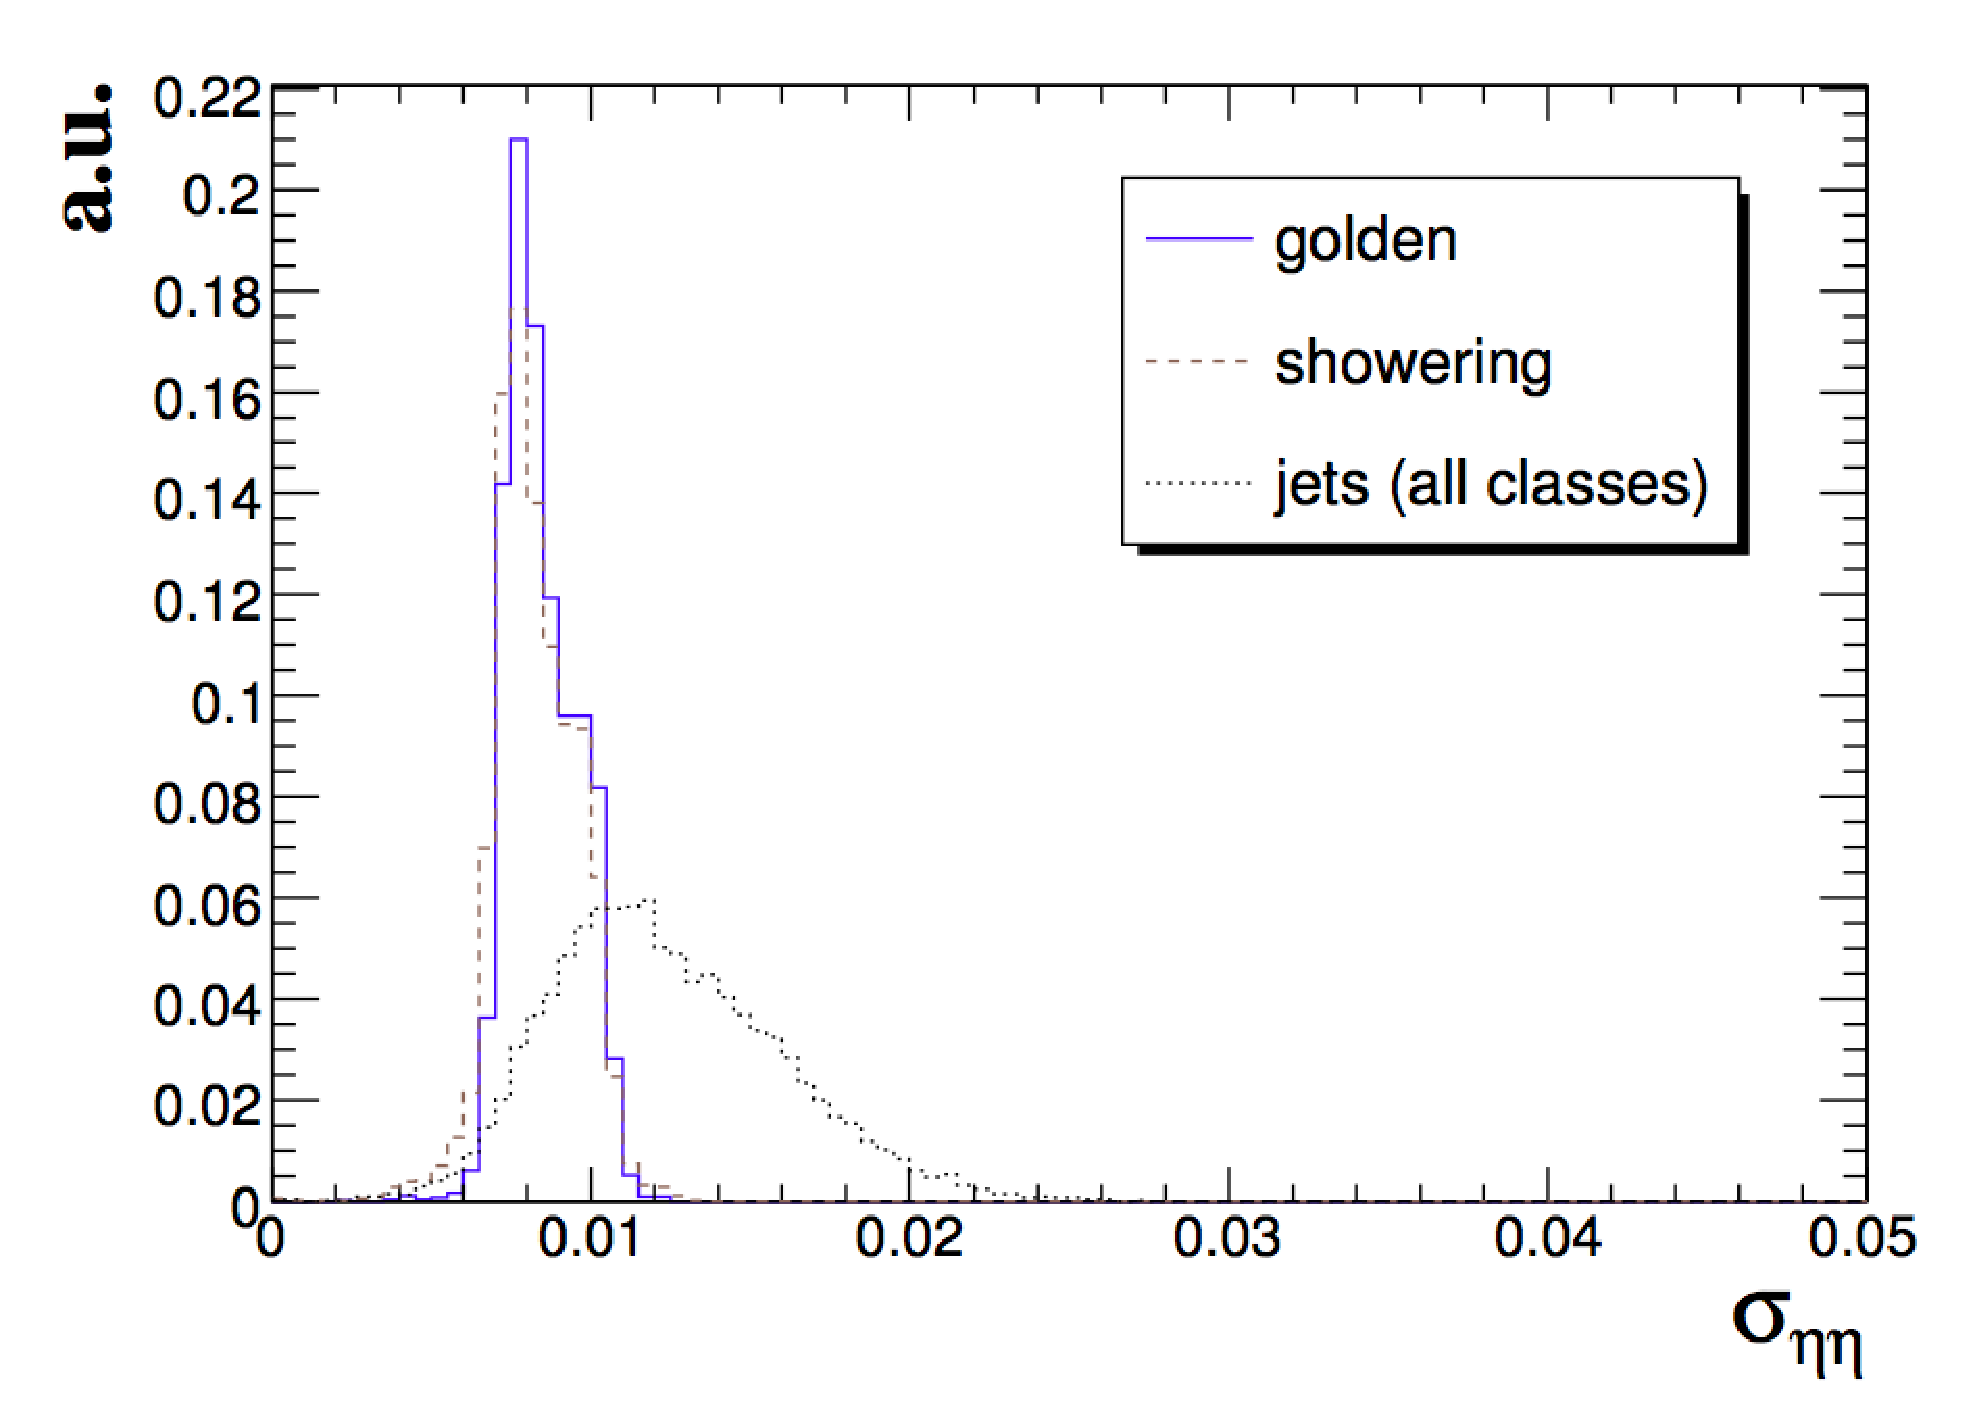
\includegraphics[width=0.5\textwidth]
      {plots/reco/elec-sigieie.pdf}}
\subfloat[]{
    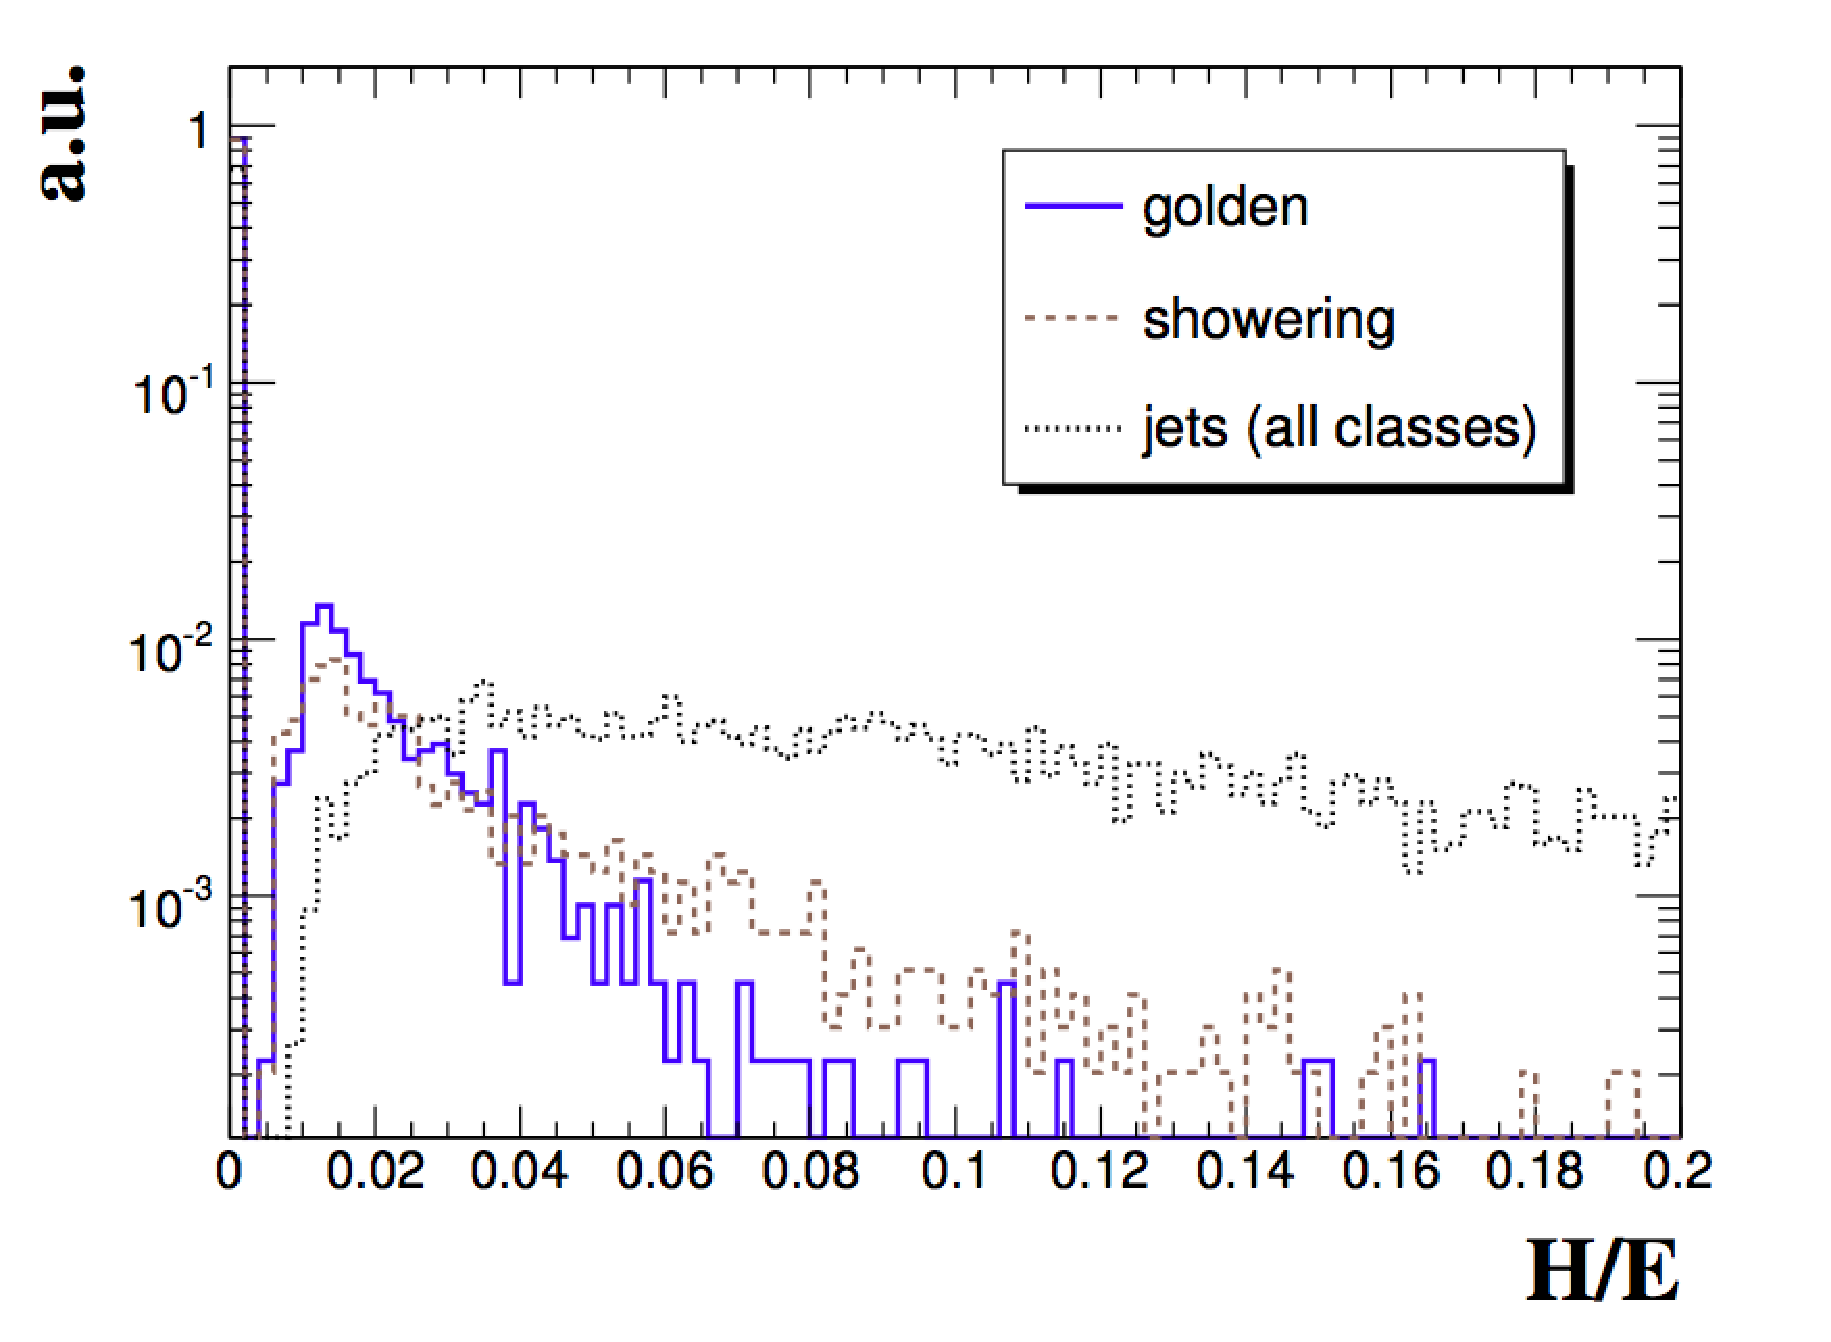
\includegraphics[width=0.5\textwidth]
      {plots/reco/elec-HE.pdf}} 
\end{center}
\caption{
    Plots showing: the separation in a) $\phi$ and b) $\eta$ between the supercluster and the
    track direction, c) the energy-weighted $\eta$ width of the cluster and d)
    the ratio of hadronic and electromagnetic energy in the region of the seed
    cluster. Plots are shown for electrons and backgrounds from jets. 
}
\label{fig:electronID}
\end{figure} 

The $\PH \to \Pgt\Pgt$ analysis makes use of these four variables and additional
conditions on the track quality and kinematics \cite{Baffioni:2006cd} to provide
improved identification efficiency. These variables are combined in a
multivariate \ac{BDT} \cite{TMVA}, which is trained in two bins of
$\pt$ and three bins of $\eta$ using $Z/\gamma^{*} \to \Pe\Pe$ events in data.
The additional variables used as inputs to the \ac{BDT} are as follows:

\begin{itemize}
\item Quantities relating to the quality of the tracks, including the normalised
$\chi^{2}$ and the number of valid hits in the track fit.
\item Additional quantities to the above relating to the cluster shape, including the
variable $f_{e}=1-e_{1\times5}/e_{5\times5}$, in which $e_{1\times5}$
($e_{5\times5}$) denotes the energy deposited in an array of $1 \times 5$ ($5
\times 5$) cells in the vicinity of the supercluster seed, and the variable
$R_{9}$, which gives the fraction of the supercluster energy in an array of
$3\times3$ cells in the vicinity of the supercluster seed.  
\item Additional variables relating to the compatibility of the hadronic and EM
energy with the track momentum, including the ratio of supercluster energy over
the momentum of the associated track evaluated at the \ac{PV} (E/P), the
quantity $1/E-1/p$ which quantifies the energy-momentum compatibility, the ratio
of the electron cluster energy to the momentum of the associated track evaluated
at the surface of the calorimeter and the ratio of the energy reconstructed in
the pre-shower detector over the raw energy of the supercluster.  
\end{itemize}

The \ac{BDT} output is then a $\pt$ and $\eta$ dependent cut threshold. Finally
non-prompt electrons from photons interacting with the tracker are suppressed
by requiring there are no missing hits in the inner tracker and that the
electron is not matched to a reconstructed conversion. The electron must also be
consistent with the \ac{PV}, by having small impact parameters. More information
on the efficiency of the electron ID in the $\PH \to \Pgt\Pgt$ analysis can be
found in section \ref{sec:datamcfactors}.

\section{Muons}
\label{sec:muons}

Muons typically travel through the CMS calorimeters with minimal energy deposit
and are reconstructed in the muon chambers. Thus we are able to reconstruct
muons in two independent places - the tracker and the muon chambers. This
greatly improves the ability to isolate muons from hadronic activity. The
``global'' muon reconstruction algorithm \cite{MuonReco} uses both sets of information by
starting from each track in the muon chambers and searching for a compatible
track in the inner tracker. If a compatible track is found, the energy and
momentum of the muon is determined by a fit to the hits in both the inner
tracker and the muon chambers, taking into account the expected energy loss
within the magnet. This improves the momentum resolution compared to
the track only measurement for muons with $\pt$ larger than 200 $\GeV$. For
lower $\pt$ muons, the momentum resolution is driven by the fit to the tracker
hits. For low $\pt$ muons ($< 5~\GeV$), the reconstruction starting from the inner
tracker is more efficient due to the lower probability of these muons reaching
the muon chambers. This is known as ``tracker'' muon reconstruction.  

Backgrounds to prompt muons consist of non-prompt muons from in-flight decays of
hadrons and punch-through of charged hadrons which pass through the calorimeters
into the muon chambers. These backgrounds are reduced through the use of ID
requirements based on the properties of the muon track. In flight decays are
reduced by the requirement of hits in at least one pixel detector and $5$
tracking layers. The $\chi^{2}$ of the global track fit must be better than
$10$, and the global track fit must include hits from at least one segment in
the muon detector, both of which provide rejection of punch-through hadrons. In
addition, track segments must be found in at least two stations of the muon
detector. These conditions taken together provide the ``tight'' muon ID used in
many analyses, including the $\PH\to\Pgt\Pgt$ analysis.
The efficiency of CMS muon reconstruction is found to be better
than $96\%$ for muons with $\pt > 10~\GeV$. Some studies of the ID efficiency of
muons in data and \ac{MC} in the context of the $\PH \to \Pgt\Pgt$ analysis can
be found in section \ref{sec:datamcfactors}.

\section{Lepton Isolation}
\label{sec:leptonisolation}

In order to further reduce background contributions from mis-identified \ac{QCD} jets,
electrons and muons are required to be isolated. Isolation is computed as the
scalar sum of transverse momenta of the candidates within a cone in
$\eta-\phi$ space of size $\Delta R = 0.4$ centred on the lepton direction. 
This sum includes all charged particles, neutral hadrons and photon candidates. 
To reduce the contamination of particles which originate from \ac{PU} events 
in this cone, charged  candidates with an impact parameter greater than 
$0.1~\cm$ from the primary vertex are excluded from the sum. An estimate of the 
neutral pileup contribution is made based on the charged pileup contamination,
multiplied by a factor 0.5, which is approximately the ratio of neutral to
charged components of the hadronisation, as determined from simulation.   
The isolation is then defined as follows:

\begin{equation}
I = \sum^{\substack{\text{charged} \\ \text{non-pileup}}}\pT +
\text{max}\left(0,\sum^{\text{neutral}}\pT+\sum^{\text{photon}}\pT-\frac{1}{2}\sum^{\substack{\text{charged}
\\ \text{pileup}}}\pT\right).
\end{equation}

Then requirements are usually placed on relative isolation, defined as
$I / \pt^{\text{lepton}}$. In the $\PH\to\Pgt\Pgt$ analysis the electrons and
muons are both required to have $I / \pt^{\text{lepton}} < 0.1$. 

\section{Jets}
\label{sec:jets}

Jets result from the large numbers of quarks and gluons present in a hadron
collider. The term `jet' is used to refer to the collimated shower of particles
which is produced from the hadronisation of such a quark or gluon. In order to
reconstruct the original parton, these showers of particles need to be collected
and combined correctly. Before describing exactly how this is done, section
\ref{sec:particleflow} decribes an important algorithm which greatly improves
this reconstruction. 

\subsection{Particle Flow}
\label{sec:particleflow}

CMS uses a \ac{PF} \cite{CMS-PAS-PFT-09-001,CMS-PAS-PFT-10-001,CMS-PAS-PFT-10-002} 
algorithm to combine the individual track and energy deposits in each sub-detector. 
This allows the reconstruction of individual particles emerging from all vertices: charged
hadrons, neutral hadrons, photons and the muons and electrons already discussed.
These particles can then be 
used to calculate the missing transverse energy $\MET$,
reconstruct jets and quantify the isolation of leptons and photons. A separate
algorithm is used to reconstruct hadronic decays of taus, discussed in section
\ref{sec:taus}. 

The success of the \ac{PF} algorithm is to combine the high resolution of
the tracker with the energy resolution and high granularity of the calorimeters.
The output of the algorithm is a set of the stable particles in the event
resulting from the hard interaction, from the inputs of charged particle tracks,
calorimeter energy deposits and muon chamber hits. The clustering of energy
deposits is performed separately in the \ac{ECAL} and \ac{HCAL}, for electrons
as discussed in section \ref{sec:electrons} this allows the combination of
bremsstrahlung photons with the parent electrons and in the \ac{HCAL} this
allows the separation of the neutral and charged hadrons. The clustering
proceeds by first defining a cluster seed, which corresponds to the calorimeter
cell with the highest local energy. The threshold for clustering neighbouring
cells is that they must have energy greater than 2 standard deviations above
noise level. After the clustering, the different \ac{PF} elements are linked into
blocks to be interpreted as a particular particle. This can be done using
extrapolation of tracks into the calorimeters, where the two elements are linked
if the track falls inside the cluster volume.

\subsection{Jet Identification by Clustering}
\label{sec:jetID}

Jets are composed of a wide range of particle types which interact in the
detector in different ways. These particles must be combined using a clustering
algorithm. The choice of algorithm defines how the particles should be combined
taking into account the distance between the objects. In particular the
algorithm should be infrared- and collinear- safe, meaning that the jet
reconstruction is not affected by soft \ac{QCD} radiation or gluon splitting.
The algorithm used for the
analyses in this thesis is the `anti-$k_{\text{T}}$' algorithm as implemented in
the \textsc{fastjet} package \cite{Cacciari:fastjet1}, which considers all 
objects within a certain jet `size' defined by a parameter $R=0.5$, and 
sequentially combines them starting from the one with the
smallest distance from the beamline. If this distance is smaller than the
distance between this object and the closest second object then the first is
taken to be a final state jet and removed from the object list,
otherwise the two objects are combined into one and the process repeats. 
This process is repeated for all objects until none remain in the list. The effect of this
is to form a cluster around the hardest particles in a cone in $\eta$-$\phi$.

Jet identification criteria are applied to reduce the contribution of jets from
noise in the calorimeters. These include the following:
\begin{itemize}
\item Jets must consist of at least one \ac{PF} component. 
\item It is required that the jet energy has contributions
from both the \ac{ECAL} and \ac{HCAL}.
\item The fraction of the total jet energy as a result of photons or neutral
hadrons should be less than 0.99 of the total jet energy.
\item Jets within the acceptance of the inner tracker must have at least one
charged object and a charged energy fraction greater than zero and an electron
energy fraction less than 0.99. 
\end{itemize}

\subsection{Jet Energy Corrections}
\label{sec:JEC}

An important aspect of jet identification is the correct measurement of the jet
energy, which is typically different between reconstructed and true hadron-level jet energy
due to experimental effects. This can be due to uninstrumented regions of the
detector, non-linear calorimeter responses and contamination by jets from \ac{PU}
interactions. Particles from different \ac{PU} vertices can be clustered and identified as a
jet, or overlap with a jet from the primary vertex affecting the measurement of the jet energy.
Pileup jet identification \cite{CMS-PAS-JME-13-005} is used to classify these events, which consists
of a \ac{BDT} \cite{TMVA} with input variables such as
momentum and spatial distribution of the jet particles. In addition
a calibration factor is applied to account for imperfections in the
neutral-hadron calibration, the jet energy containment and small differences
between the simulated and observed response.

To correct for remaining \ac{PU} and the other detector effects, a correction to the jet energy
scale is derived \cite{CMS-JME-10-011}:

%Read this paper when you have internet and find a better way to write this
%equation

\begin{equation}
P_{\text{corr}}^{\mu} = C_{\text{PU}}(\pT^{\text{raw}},\eta) \cdot
C_{\text{rel}}(\pT^{\text{PU}},\eta) \cdot C_{\text{abs}}(\pT^{\text{rel}},\eta) \cdot
P_{\text{raw}}^{\mu}\, .
\end{equation}

In this equation, $C_{\text{PU}}$ is the correction for \ac{PU},
$C_{\text{rel}}$ is a relative correction and $C_{\text{abs}}$ is an absolute
correction. The corrections are applied sequentially such that the \ac{PU}
correction is a function of raw jet $\pt$ ($\pt^{\text{raw}}$),
the relative correction is a function
of the $\pt$ corrected for the pileup effects ($\pt^{\text{PU}}$) and finally
the absolute correction is a function of the relative-corrected $\pt$
($\pt^{\text{rel}}$). All of the corrections are applied as a function of
jet $\eta$. These subsequent corrections are applied to the raw
4-vector of the jet $P_{\text{raw}}^{\mu}$ to yield the corrected 4-vector
$P_{\text{corr}}^{\mu}$.

The \ac{PU} correction is determined using the $\pt$ density in the event to
estimate the contribution from \ac{PU} on a per-jet basis. The relative
correction is determined using a dijet $\pt$ balance method which uses dijet
events containing a jet with $|\eta| < 1.3$ and exploits momentum conservation.
The probe jet (which can have any value of $\eta$), is used to calculate the
average of a balance quantity, defined as:
$(\pT^{\text{probe jet}}-\pT^{\text{ref jet}})/\pT^{\text{average}}$, in bins of
average dijet $\pt$ and probe $\eta$. Figure \ref{fig:jetresponse} shows the
values of the response for \ac{MC} and data. The absolute correction is measured
using the \ac{MPF} method \cite{Abe:1992sj}, using $\gamma$+jets and $\PZ$+jets
events and enforcing momentum conservation in light of the fact that these
events shouldn't contain any real $\MET$. Thus any measured $\MET$ can be used to
calibrate the $\pt$ of the jets. The total uncertainty on the jet energy scale
is given by the sum in quadrature of the estimated uncertainties in each of the
correction factors. This uncertainty varies between approximately $3$ and $5\%$
depending on $\pt$ and $\eta$. 

\begin{figure}
\begin{center}
\subfloat[]{
    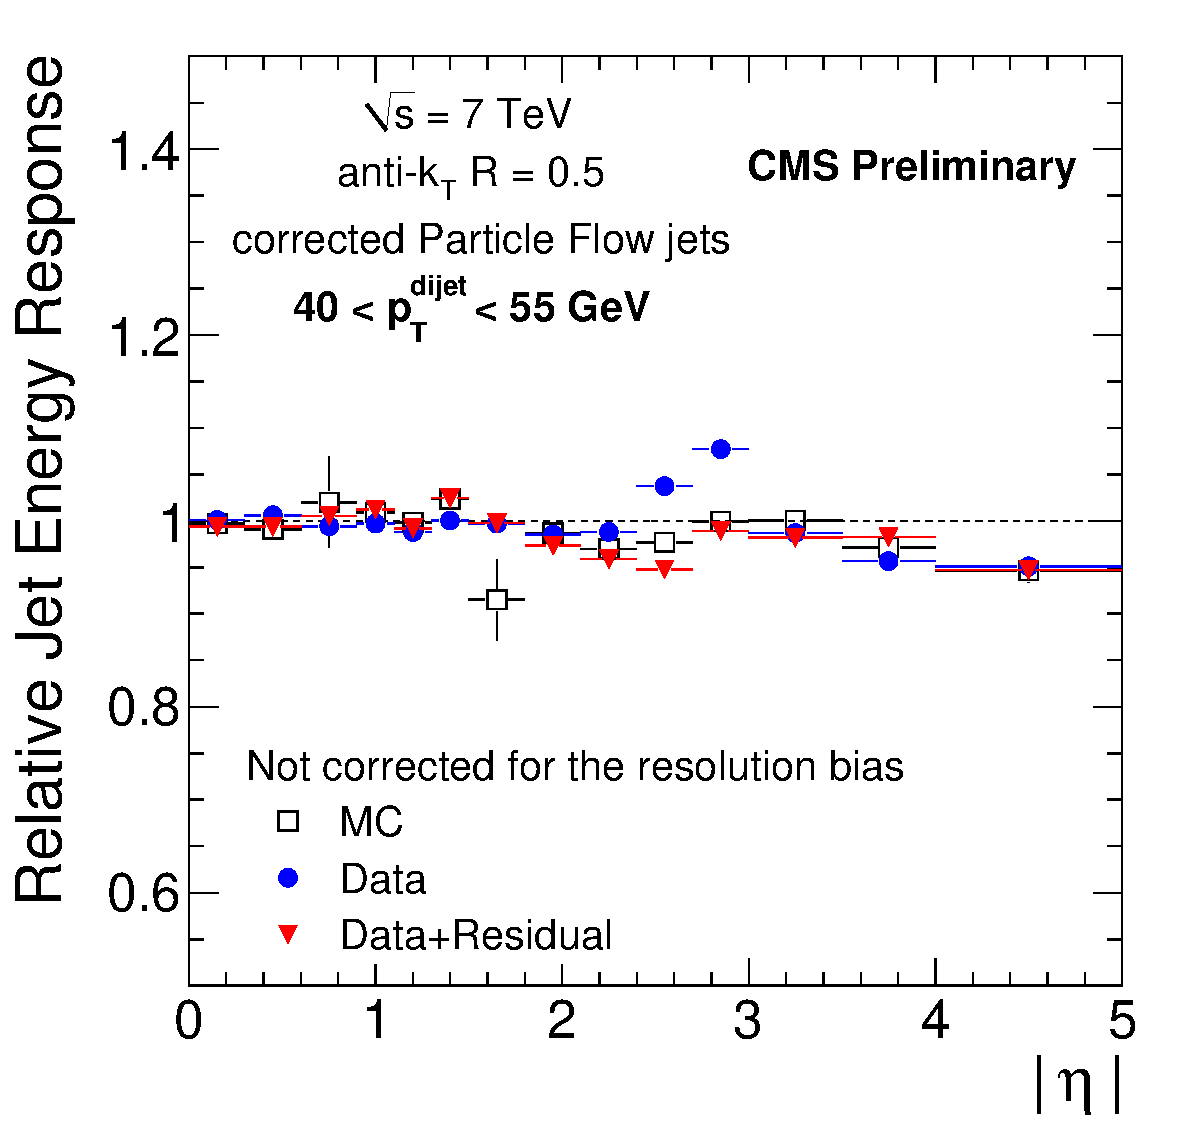
\includegraphics[width=0.5\textwidth]
      {plots/reco/jes-response-a.pdf}}
\subfloat[]{
    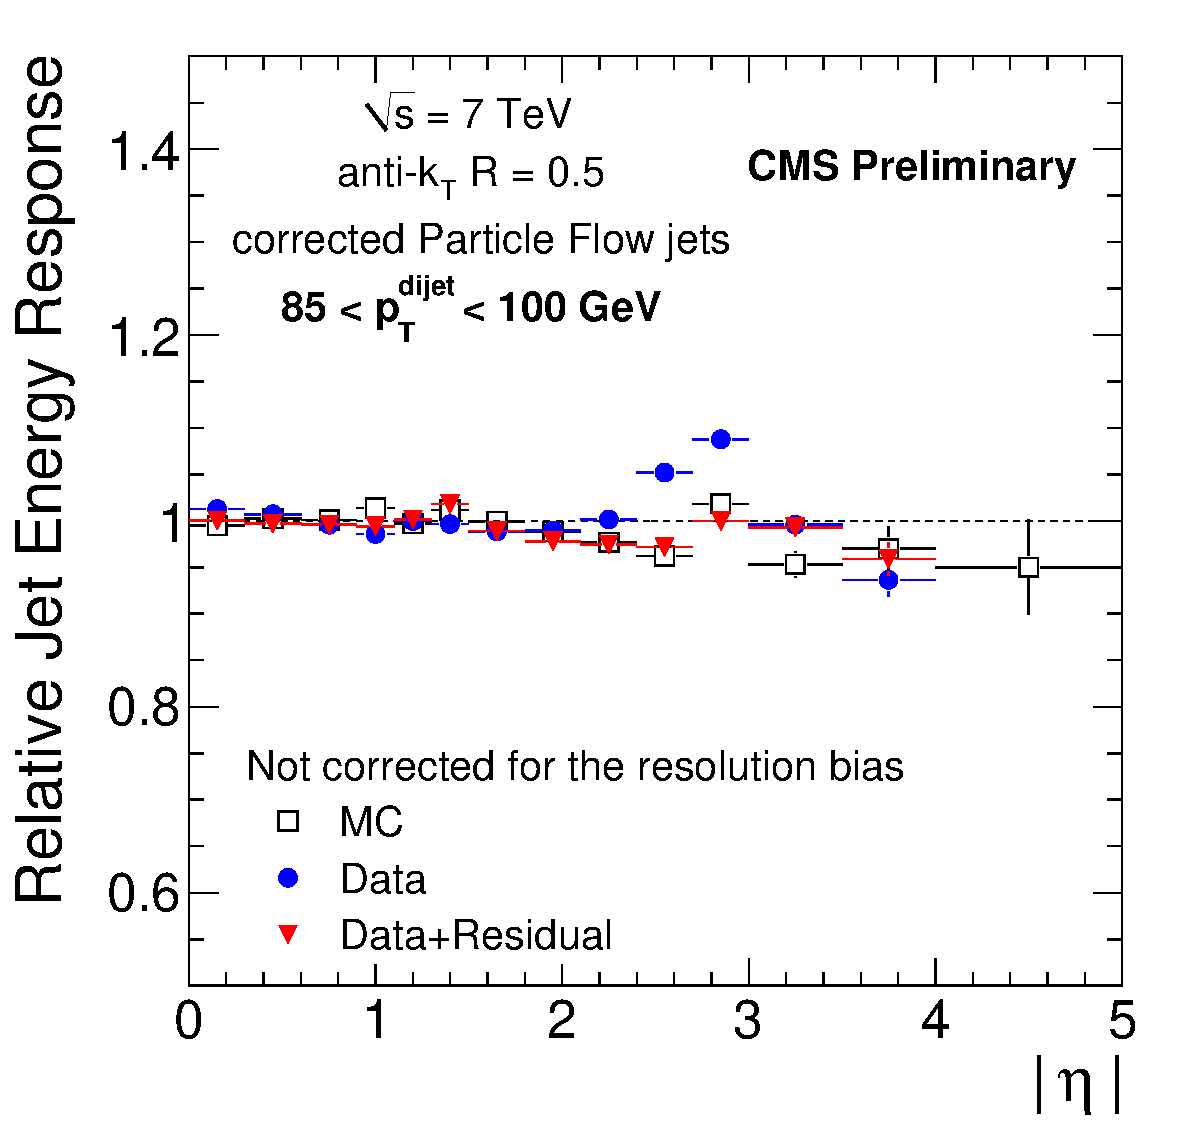
\includegraphics[width=0.5\textwidth] 
      {plots/reco/jes-response-b.pdf}} 

\end{center}
\caption{
Relative jet energy response as a function of jet $\eta$ measured in dijet
events, for jets with $40 < p_{T}^{\text{dijet}} < 55$ (left) and 
$85 < p_{T}^{\text{dijet}} < 100$ in data and MC.       
}
\label{fig:jesresponse}
\end{figure}

\subsection{B-tagged Jets}
\label{sec:btag}

The identification of jets which originate from b-quarks is important in many
\ac{SM} and \ac{BSM} processes. As a result of the fact that decays of b-quarks
are suppressed by small CKM matrix elements, b-flavoured hadrons have relatively
long lifetimes. Such hadrons are also relatively heavy due to the large mass of
the b-quark, and as such the decay products typically have large momenta
perpendicular to the b-hadron momentum direction. Both of these features are
exploited in identification of b-tagged jets.

In the $\PH \to \Pgt\Pgt$ analysis, jets originating from b-quark
hadronization are identified using the \ac{CSV} b-tagging
algorithm \cite{bjets}. The long lifetime of the b-hadrons results in a
secondary decay vertex which can be reconstructed. In the \ac{CSV} algorithm, a
jet is considered b-tagged if it has $\pT>20\,\GeV$, $|\eta|<2.4$ and a
\ac{CSV} discriminator output greater than a loose, medium or tight working
point, chosen to give different levels of ID efficiency and mis-tag rates. The
inputs to the calculation of the \ac{CSV} discriminator include secondary
vertex information and the track-based lifetime information. Two likelihoods are
built from these variables, one to discriminate between b and c jets and one to
discriminate between b and light jets. 

In the $\PH\to\Pgt\Pgt$ analysis, the medium working point of the \ac{CSV}
discriminator is used to identify b-jets, corresponding to a discriminator
output greater than 0.679. The distribution of the \ac{CSV} discriminator 
can be seen in figure \ref{fig:csv}. The medium working point corresponds to a
b-tag efficiency of $\approx 85\%$ and a mis-tag rate of $\approx 1\%$. 

\begin{figure}
\begin{center}
    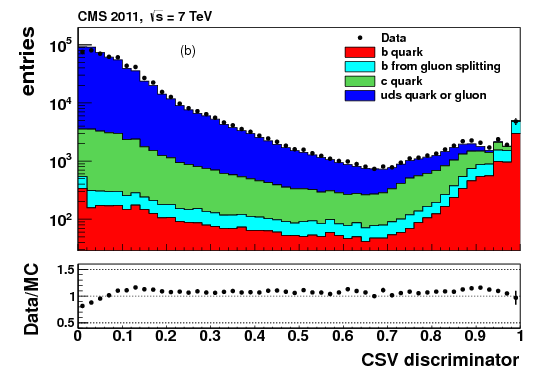
\includegraphics[width=0.6\textwidth]
      {plots/reco/csv.png}
\end{center}
\caption{
The distribution of the \ac{CSV} discriminator used to identify b-jets.    
}
\label{fig:csv}
\end{figure}


\section{$\MET$}
\label{sec:met}

Neutrinos and any other hypothetical weakly interacting stable particles do not
interact with the CMS deterctor. We infer their production from the resulting
imbalance in $\ET$ in a given event, which the hermeticity of the CMS detector
allows us to measure to a high degree of accuracy. This is crucial not only in
many searches for new physics involving such hypothetical particles, but also for
\ac{SM} processes involving neutrinos. In particular for the $\PH \to \Pgt\Pgt$
analysis accurate measurement of the $\MET$ is essential to reconstruct the
candidate taus after they decay via the weak interaction.

The \ac{PF} algorithm allows us to calculate $\MET$ as the opposite of the vectorial sum
of the transverse momenta of all \ac{PF} particles. The resolution of the $\MET$
can be degraded by a number of factors. These include minimum energy thresholds
in the calorimeters, non-instrumented detector regions and multiple \ac{PU}
interactions. The performance of the \ac{PF} $\MET$ response differs in data and
MC, and a correction is derived from an independent $\PZ\to\mu\mu$ sample which
does not contain any `real' $\MET$. The longitudinal and transverse component of
the $\pt$ response and the resolution of the $\PZ$ boson recoil is parameterised
as a function of $\pt$ and jet multiplicity. This parameterization is then
applied to all simulated events as a function of the $\pt$ of the boson. Then
finally the $\MET$ is the transverse energy of the vectorial sum of the visible
decay proucsts and the recoil as parametrised in data. 
%A number of techniques exist for correcting both the response and
%resolution of the \ac{PF} $\MET$ \cite{Chatrchyan:2011tn}. 

To further reduce the dependence of resolution on \ac{PU}, the $\PH\to\Pgt\Pgt$
analysis makes use of so-called MVA $\MET$ \cite{CMS-PAS-JME-12-002}, 
which uses a \ac{BDT} regression multivariate analysis
including the \ac{PF} $\MET$ as one input. Other inputs are versions of the
$\MET$ calculated using the following combinations of \ac{PF} particles: 
\begin{itemize}
\item charged hadrons from the primary vertex;
\item charged hadrons from the primary vertex and neutral particles in jets
passing the pileup jet ID;
\item charged hadrons from pileup vertices and neutral particles in jets failing
the pileup jet ID;
\item charged hadrons from the primary vertex and all neutral particles in the
event, to which is added the vectorial sum of the transverse momenta of neutral
particles within jets failing the pileup jet identification.
\end{itemize}

For each type of $\MET$ the recoil is calculated defined by:
\begin{equation}
\vec{u} = \MET \cdot \hat{\phi} - \sum_{i}{ \vec{\pt}^{\text{lep}}} ,
\label{eq:recoil}
\end{equation}

where $\hat{\phi}$ is the direction of the $\MET$ in the transverse plane and
$\vec{\pt}^{\text{lep}}$ is the $\pt$ vector of the leptons originating from the
hard interaction. The \ac{BDT} produces a correction to both the angle and the
magnitude of the \ac{PF} recoil. The final computed recoil is added to the
vector sum of leptons as in equation \ref{eq:recoil} and the resulting corrected
$\MET$ is then taken. 

The MVA $\MET$ has a resolution which is much less
dependent on pileup, as can be seen in figures \ref{fig:mvamet}.

\begin{figure}
\begin{center}
\subfloat[]{
    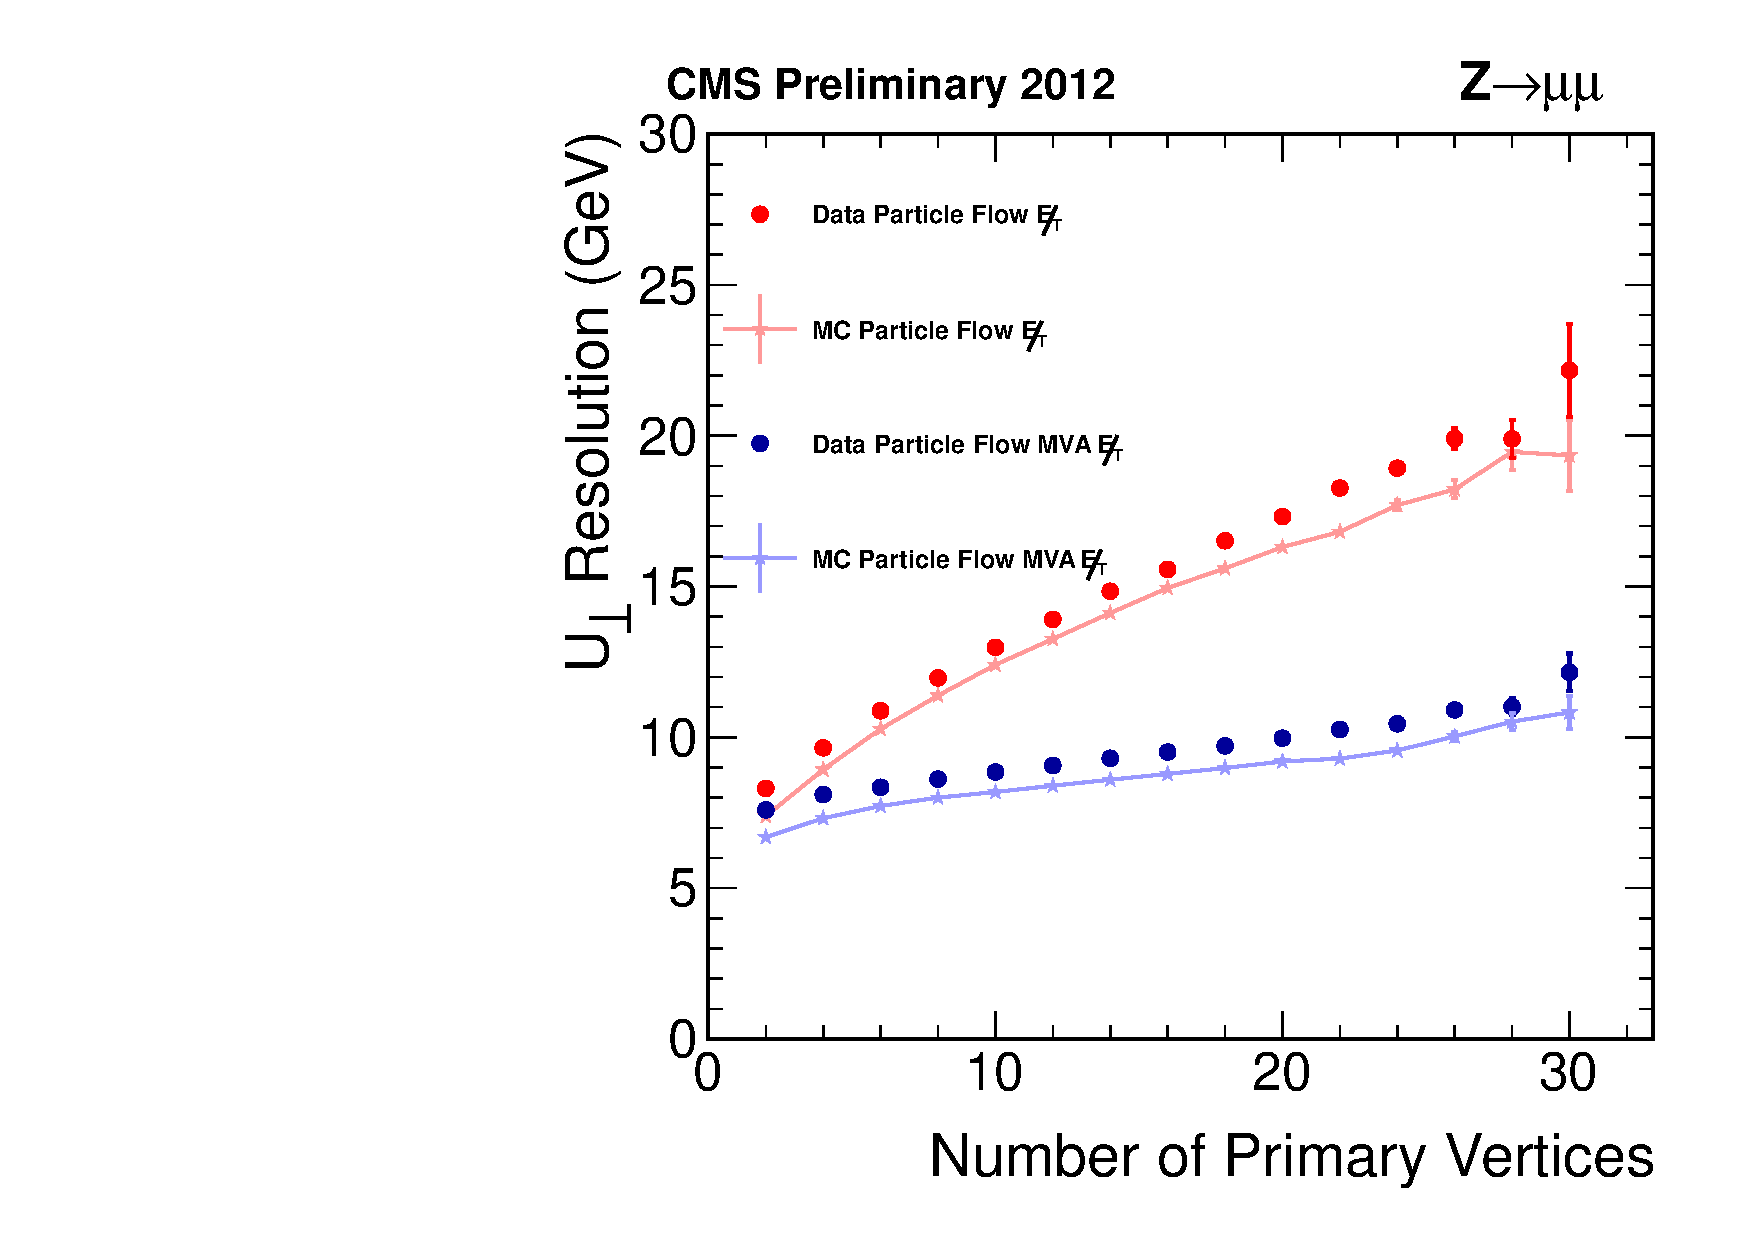
\includegraphics[width=0.5\textwidth]
      {plots/reco/U1Res.pdf}}
\subfloat[]{
    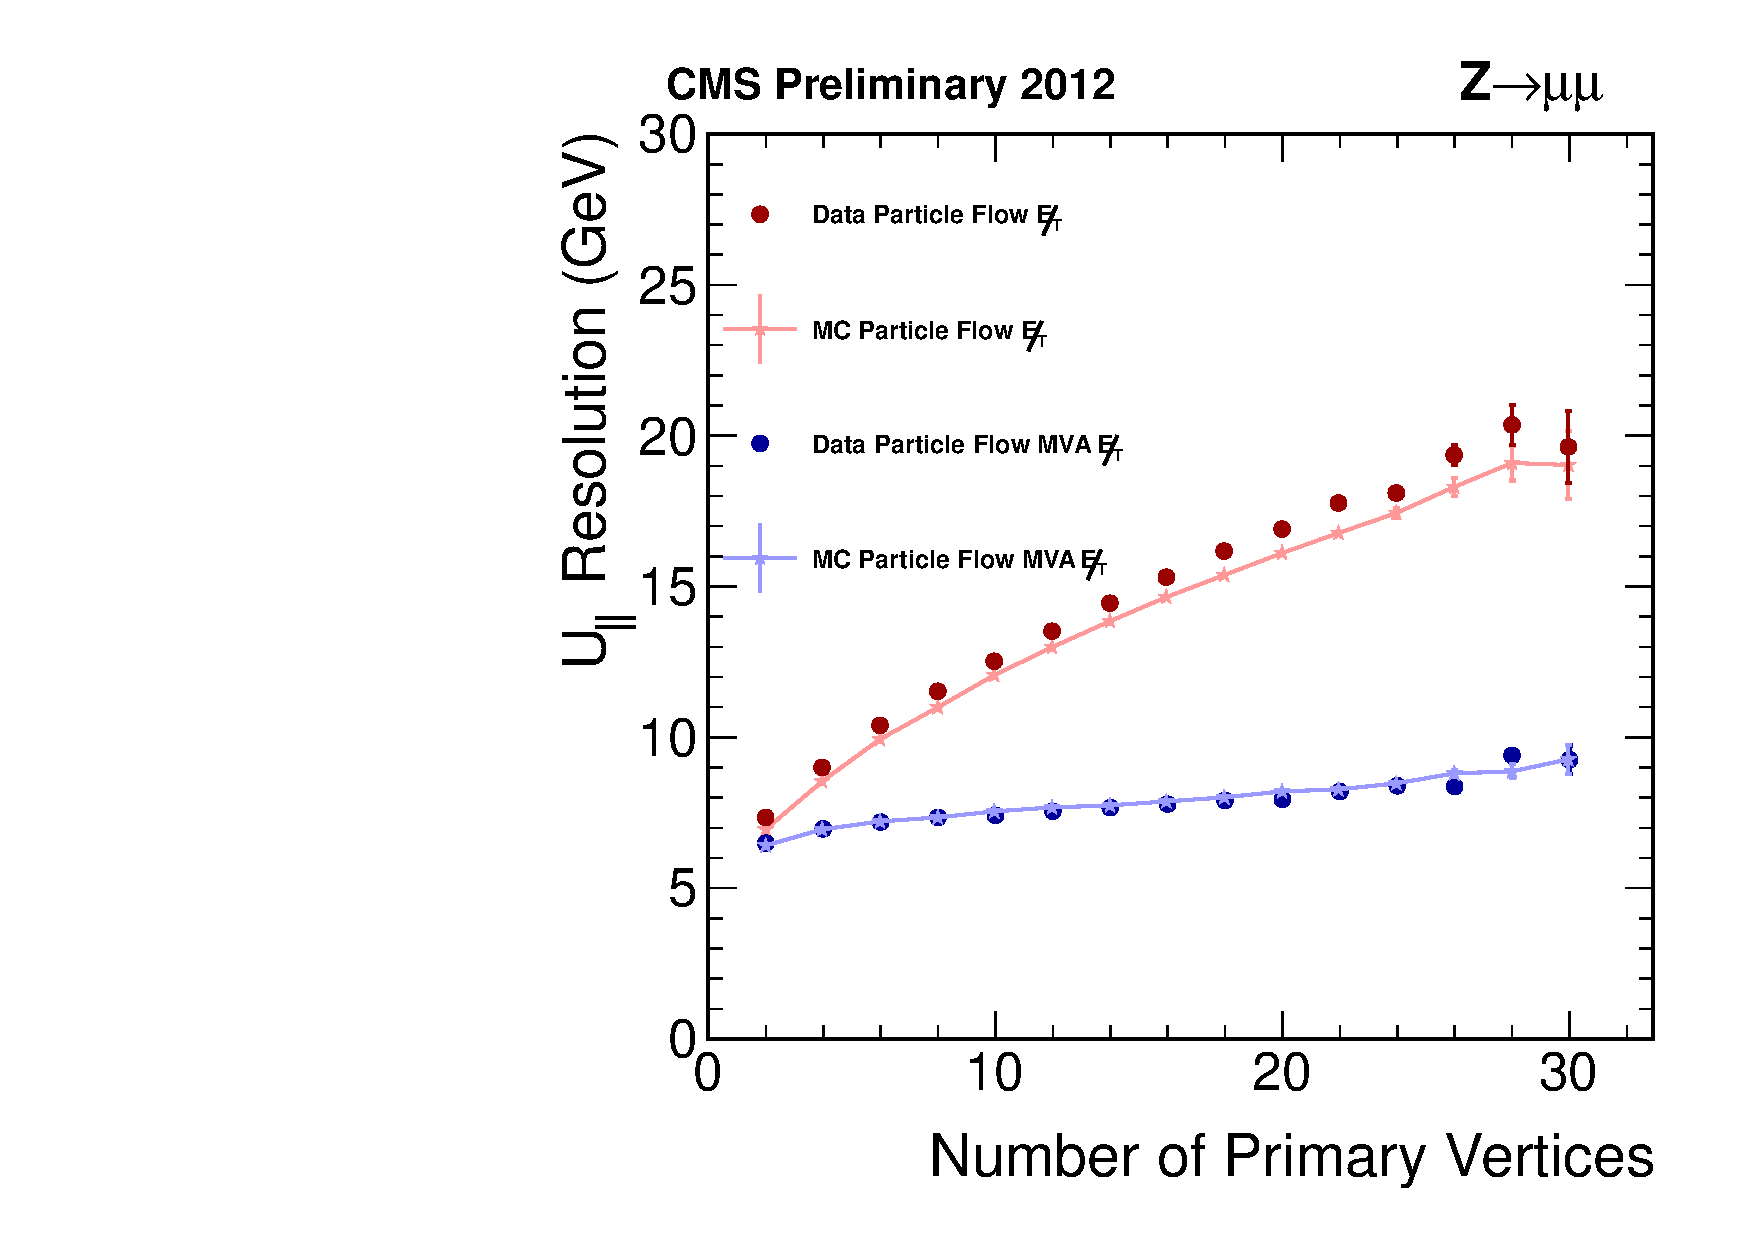
\includegraphics[width=0.5\textwidth] 
      {plots/reco/U2Res.pdf}} 
\end{center}
\caption{Plots illustrating the dependence of the resolution of the hadronic
recoil response on the number of primary vertices in the event.
}
\label{fig:mvamet}
\end{figure}

\section{Hadronic Taus}
\label{sec:taus}

Taus decay via the weak force. Approximately $35\%$ of the time, they decay into a final state consisting of a tau
neutrino, an electron/muon and the associated electron/muon neutrino. 
This section describes the identification of taus for the other $\approx65\%$ of the time,
when they decay into a tau neutrino plus quarks yielding a hadronic tau, $\tau_{h}$. The different
possibilities for hadronic tau decays are listed in table \ref{tab:hadronictaus}.

\begin{table}[bth]
\begin{tabular}{|c|c|c|}
\hline
Decay Mode & Intermediate Resonance & Branching Fraction [\%] \\
\hline
\hline
$\Pgtpm\to\Pgppm\Pgpz\Pgngt$ & $\Pgr$(770) & 26.0 \\
\hline
$\Pgtpm\to\Pgppm\Pgngt$ & -  & 11.6 \\
\hline
$\Pgtpm\to\Pgppm\Pgpz\Pgpz\Pgngt$ & $\text{a}_{1}$(1260) & 10.8 \\
\hline
$\Pgtpm\to\Pgppm\Pgpmp\Pgppm\Pgngt$ & $\text{a}_{1}$(1260) & 9.8 \\
\hline
$\Pgtpm\to\Pgppm\Pgpmp\Pgppm\Pgpz\Pgngt$ & -  & 4.8 \\
\hline
Other hadronic modes & - & 1.7 \\
\hline
\hline
Total & &  64.7 \\
\hline
\end{tabular}
\caption{List of the possible hadronic tau decay modes. The branching ratios for
each is given, and where the decay proceeds via an intermediate resonance this
is given along with its mass in $\MeV$\cite{PDG}.}
\label{tab:hadronictaus}
\end{table}

The largest fraction of hadronic decays proceeds via the $\Pgr$(770) resonance
resulting in one charged and one neutral pion. Other common modes produce
different numbers of neutral or charged pions. Decays with more than 3 charged
pions are included in the other hadronic modes listed in the table and are
relatively rare. The knowledge of the number of pions in the final state is used in the
identification of hadronic taus, using the \ac{HPS} algorithm
described in section \ref{sec:hps}.

Hadronic taus are a collection of hadronic particles and as such the first level
of identification is similar to jet ID. 
Since the decay products come directly from the tau they are constrained by the
tau mass, this results in a highly collimated hadronic system compared with the
typical jet. This allows us to differentiate hadronic taus from
quark and gluon jets. This property is utilised in the tau isolation,
described in section \ref{sec:tauisolation}.

\subsection{Hadron Plus Strips Algorithm}
\label{sec:hps}

For the $\PH \to \Pgt\Pgt$ analysis, the \ac{HPS} algorithm is used to identify
hadronic taus \cite{CMS-PAS-TAU-11-001}. The \ac{HPS} algorithm, makes us of \ac{PF} candidates to reconstruct the
charged pions and the photons resulting from the decays of the neutral pions. In
addition, the kinematic properties listed in table \ref{tab:hadronictaus} can be
applied. In this algorithm only the visible products of the taus are considered
- the tau neutrino forms part of the missing energy.

The algorithm is seeded by a \ac{PF} jet, which is reconstructed as described in
section \ref{sec:jetID} with distance parameter $R=0.5$. The photons from the neutral pion decay have a high
probability to convert to electron-positron pairs within the tracker, resulting
in an EM shower spread in the $\phi$ direction. These candidates are clustered
using strips with size $\Delta\eta = 0.05$ and $\Delta\phi = 0.2$ initially
centred on the most energetic EM candidate in the \ac{PF} jet. Strips with
$\pt>1~\GeV$ are considered. The energy of the
strip is required to be consistent with the mass of the neutral pion, and hence
between 50 and 200 $\MeV$. The strips are then combined with the charged hadrons
from \ac{PF} to give us 4 different cases:

\begin{itemize}
\item Single charged hadron or "prong", no strips: corresponds to $\Pgtpm\to\Pgppm\Pgngt$,
with some contribution from $\Pgtpm\to\Pgppm\Pgngt\Pgpz$ in the case that the
neutral pion is not energetic enough to be detected.
\item Single charged hadron or "prong", one strip: this selects decays to the intermediate
resonance of $\Pgr$(770), $\Pgtpm\to\Pgrpm\Pgngt\to\Pgppm\Pgpz\Pgngt$. In this
case the combined system must have invariant mass consistent with the
$\Pgr$(770).
%or $\text{a}_{1}$(1260), so between 300 and 1300 $\MeV$. %check - is the lower
%bound 300 or 400? 
\item Single charged hadron or "prong", two strips: corresponds to
$\Pgtpm\to\Pgppm\Pgpz\Pgpz\Pgngt$. Here, consistency of the mass with the
$\text{a}_{1}$(1260) resonance is required. 
\item Three charged hadrons or "prongs": these correspond to
$\Pgtpm\to\Pgppm\Pgpmp\Pgppm\Pgpz\Pgngt$ or $\Pgtpm\to\Pgppm\Pgpmp\Pgppm\Pgngt$. 
In this case, the tracks are required
to come from the same vertex, with a minimum inpact parameter in the tranverse
plane of $2~\mm$. The three candidates must also have total charge of 1, and a
mass consistent with $\text{a}_{1}$(1260). 
\end{itemize}

In all of the above cases, the charged hadrons and strips must be contained
within a cone defined by $\Delta R=2.8~\GeV/\pt^{\tau_{h}}$, where
$\pt^{\tau_{h}}$ is the $\pt$ of the hadronic tau candidate, for taus with $28 <
\pt^{\tau_{h}} < 56~\GeV$. For taus with $\pt^{tau_{h}} < 28~\GeV$ the cone is
is fixed at 0.1 and for taus with $\pt^{\tau_{h}} > 56~\GeV$ at 0.05. 
Figure \ref{fig:taudecaymode} illustrates the number of events reconstructed in
each of the tau decay modes in the backgrounds to the $\PH \to \Pgt\Pgt$ analysis.

\begin{figure}
\begin{center}
    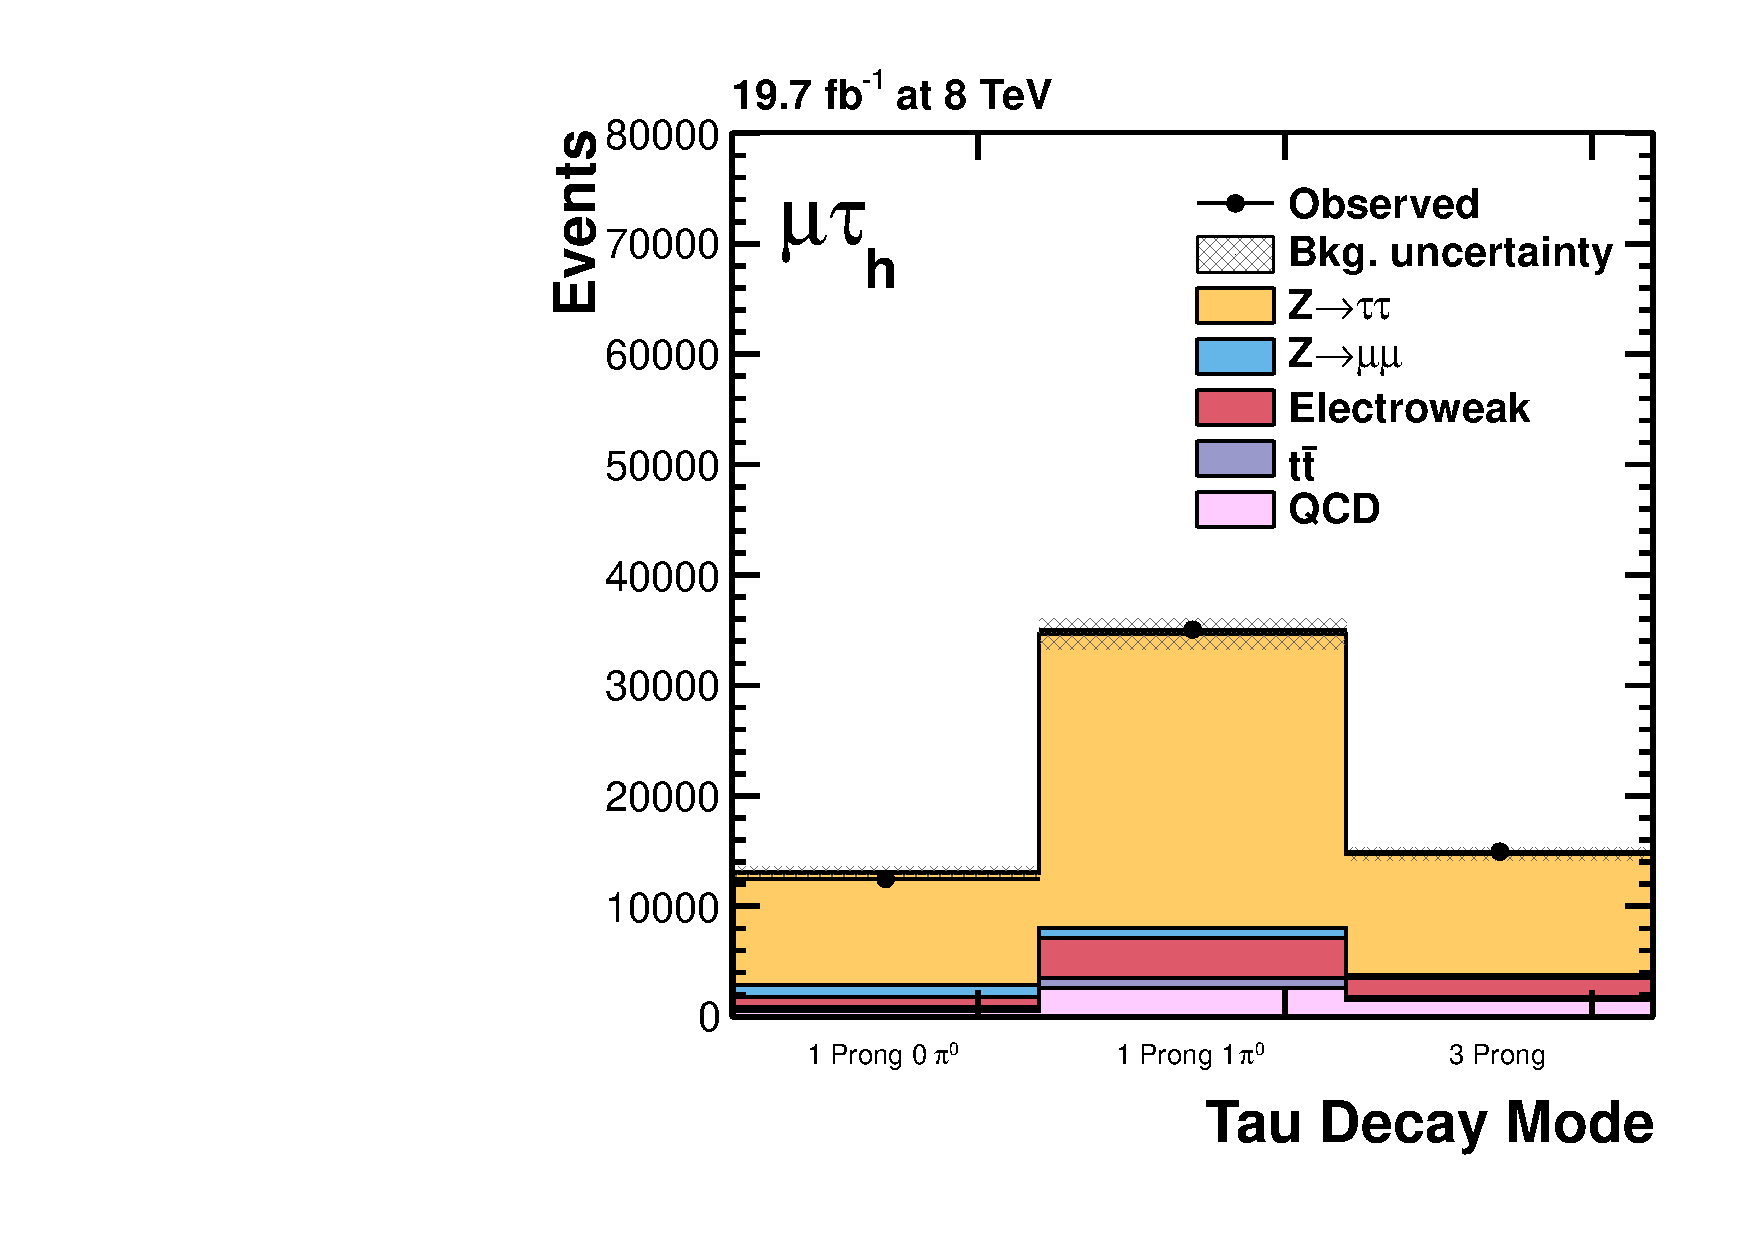
\includegraphics[width=0.5\textwidth]
      {plots/reco/tau_decay_mode_inclusive_mt_2012.pdf}
\end{center}
\caption{Plot illustrating the fraction of events in each tau decay mode in the
$\mutau$ channel of the $\PH\to\Pgt\Pgt$ analysis. The term "prong" refers to a
charged hadron. The "1 prong 1 \Pgpz" bin contains both single charged hadron
with one strip and single charged hadron with two strips, defined in the text.
}
\label{fig:taudecaymode}
\end{figure}

\subsection{Isolation}
\label{sec:tauisolation}

A measure of the isolation of the hadronic tau candidate is used to exploit the
collimated nature of the $\tau$-jets to reduce the background from quark and gluon
jets. The isolation is similar to that used for electrons and muons described in
section \ref{sec:leptonisolation}. The isolation variable is constructed from 
the sum of the $\pt$ of the
hadronic and photon \ac{PF} candidates with $\pt > 0.5~\GeV$ within a cone centred on 
the $\tau_{h}$ with size $\Delta R = 0.5$. The charged hadrons in the sum are
required to have $\Delta z < 2\mm$ with respect to the production vertex of the
$\tau_{h}$. The charged hadrons associated with other vertices (i.e. with
$\Delta z > 2\mm$) are used to
estimate and subtract the contribution to the isolation from photons produced in
\ac{PU} interactions. The isolation variable is therefore given by:

\begin{equation}
I_{\tau} = \sum \pt^{\text{charged}} + \max \left( \pt^{\gamma} - \Delta \beta,
0 \right) , 
\label{eq:tauIsolation}
\end{equation}

Where $\pt^{\text{charged}}$ is the $\pt$ of charged hadrons with $\Delta z < 2~\mm$, and
$\Delta \beta$ is the \ac{PU} correction given by the sum of charged hadrons with $\Delta
z > 2~\mm$ within a cone of $\Delta R = 0.8$ multiplied by a factor ($\approx$0.45) which is the
ratio of photons to charged hadrons in minimum bias events. Different working
points of the value of $I_{\tau}$ are chosen to correspond to loose, medium and
tight working points of tau isolation.

\subsection{Electron and muon rejection}

An electron can be misidentified as a hadronic tau with one charged hadron when
it has an isolated energy deposit in the calorimeters. Electrons can also be
reconstructed as hadronic taus when they emit photons via bremmstrahlung in the
one charged hadron plus strips modes. A \ac{BDT} is trained to reduce
misidentified electrons, using many of the same variables exploited in electron
ID. The $\PH\to\Pgt\Pgt$ analysis makes use of this discriminator in the tight
working point, which reduces the rate of misidentified electrons to around
$3\%$. 

The probability of a muon to produce a fake hadronic tau is much lower. Such
cases are suppressed by requiring that the track of the leading charged hadron
constituent in the hadronic tau is not also reconstructed as a tracker muon.
Loose, medium and tight working points are available for this discriminator
also, depending on how strict the criteria are in determining whether or not
this track matches a signal in the muon systems. 

\subsection{Energy Scale}

As in the case of jets, corrections are needed to ensure that the energy scale
of hadronic taus in \ac{MC} matches that in data. For the $\PH \to \Pgt\Pgt$
analysis this is done by fitting the tau mass distribution separately for each
decay mode for different ranges of tau $\pt$, allowing the tau energy scale to
float freely in each fit. The result is a set of $\pt$ and decay mode dependent
corrections which are applied to MC. Figure \ref{fig:taumass} shows the tau
mass distribution for the $\mutau$ channel of the $\PH\to\Pgt\Pgt$ analysis. 

\begin{figure}
\begin{center}
    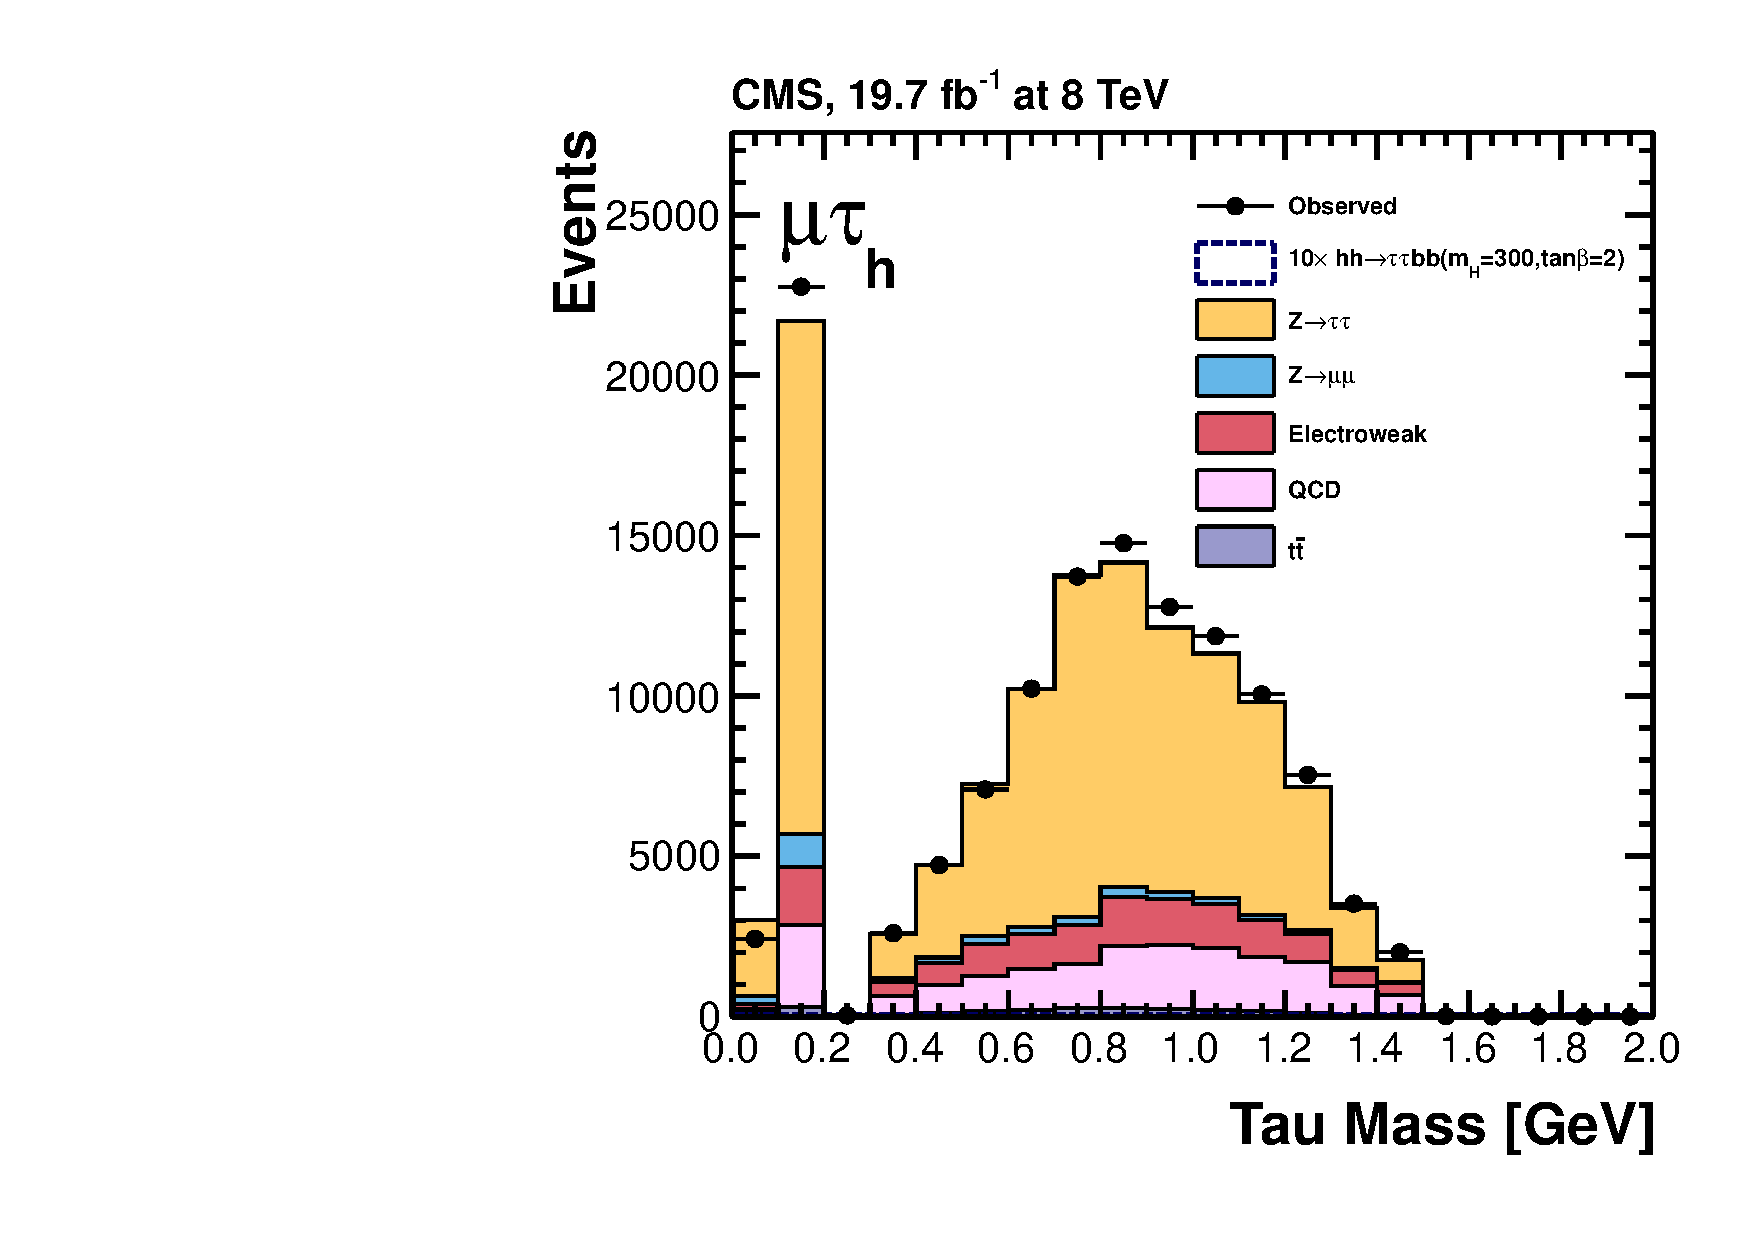
\includegraphics[width=0.5\textwidth]
      {plots/reco/m_2_inclusive_mt_2012.pdf}
\end{center}
\caption{The invariant mass of the hadronic tau in $\mutau$ channel events of
the $\PH\to\Pgt\Pgt$ analysis.}
\label{fig:taumass}
\end{figure}

\section{Di-tau Mass Reconstruction in $\PH \to \Pgt\Pgt$}
\label{sec:svfit}

In $\PH \to \Pgt\Pgt$ events, evaluation of the mass of the Higgs requires reconstruction of the 
full di-tau mass. This is important in distinguishing possible $\PH\to\Pgt\Pgt$
events from, for example, the irreducible $\PZ \to \Pgt\Pgt$ process. 
The reconstruction of the tau pair is made less straightforward
by the fact that the taus themselves decay. We can simply combine the visible
products of leptons or hadronic taus to evaluate a quantity known as visible mass,
but greater accuracy is achieved if the full mass can be reconstructed including the
invisible neutrinos. This can be achievied using a likelihood based algorithm called
SVFit, which combines the visible decay products and the reconstructed $\MET$. A
short description of this method is given in this section. A more detailed
description can be found in \cite{HIG-13-004}.

The inputs to the SVFit algorithm are the kinematics of the visible decay
products and the missing transverse energy. If all visible components of a
hadronic tau decay are treated as a single composite object, the visible part of
the decay is specified by five parameters, which are chosen to be the momentum,
polar and azimuthal angles in the lab frame, and two decay angles in the rest
frame of the tau lepton. The invisible component of the decay adds another
degree of freedom, which is chosen to be the invariant mass of the invisible
system. Leptonic tau decays produce an additional neutrino, and so an additional
variable is required which is chosen to be the invariant mass of the
two-neutrino system. The unknown parameters are constrained by three
observables: the momentum, polar and azimuthal angles of the visible products
measured in the lab frame. Further constraints are provided by
$E_{x}^{\text{miss}}$ and $E_{y}^{\text{miss}}$, the x and y components of the
$\MET$, within the experimental resolution possible. This leaves either 2 or 3 
unconstrained parameters for the hadronic or leptonic tau decay respectively. 
These are chosen to be the following:

\begin{itemize}
\item $x$: the fraction of the energy of the tau carried by the visible decay
products in the lab frame.
\item $\phi$: the azimuthal angle of the tau in the lab frame. 
\item $m_{\nu\nu}$: the mass of the neutrino system. This is set to zero for hadronic tau
decays which have only one neutrino.
\end{itemize}

The SVFit algorithm employs a likelihood approach, in which possible
$M_{\tau\tau}$ values are reconstructed by combining $E_{x}^{\text{miss}}$ and
$E_{y}^{\text{miss}}$ with a probability model with terms to account for the tau
decay kinematics and $\MET$ resolution. We define the vector $\vec{a}$ to
specify the kinematics of the tau decay as $\vec{a} =
\left(x_{1},\phi_{1},m_{\nu\nu}^{1},x_{2},\phi_{2},m_{\nu\nu}^{2}\right)$. Then the
probability that we observe the values of $\vec{x} = \left(E_{x}^{\text{miss}},
E_{y}^{\text{miss}}\right)$, given that the momenta of the visible decay products are
equal to the observed $\vec{y} = \left(p_{1}^{vis},p_{2}^{vis} \right)$,
yielding a value of $M_{\Pgt\Pgt}$ is given by: 

\begin{equation} \label{eqn:svfit-prob}
P(M_{\Pgt\Pgt}^{i}) = \int\delta\left(M_{\Pgt\Pgt}^{i} -
M_{\Pgt\Pgt}(\vec{y},\vec{a})\right)p(\vec{x},\vec{y},\vec{a})\,\text{d}\vec{a}\,
.
\end{equation}

for a series of mass hypotheses $M_{\Pgt\Pgt}^{i}$. The best estimate for the
value of $M_{\Pgt\Pgt}$ is the value which maximises this probability. 

Likelihood functions are used to model the tau decay kinematics. These are
different for hadronic and leptonic tau decays. For hadronic tau decays, a model
based on two-body phase space is used\cite{PDG}, in which all the decay products of the
tau are grouped to be one particle:

\begin{equation}
\mathcal{L}_{\Pgt}^{\text{had}} = \frac{\text{d}\Gamma}{\text{d}x\,\text{d}\phi}
\propto \frac{1}{1 - m_{\text{vis}}^{2} / m_{\Pgt}^{2}},
\end{equation}

which is valid in the physically allowed region of $m_{\text{vis}}^{2} /
m_{\Pgt}^{2} \leq x \leq 1$. The leptonic function is derived using a matrix
element approach from \cite{TauPol}:

\begin{equation}
\mathcal{L}_{\Pgt}^{\text{lep}} =
\frac{\text{d}\Gamma}{\text{d}x\,\text{d}m_{\nu\nu}\,\text{d}\phi} \propto
\frac{m_{\nu\nu}}{4m_{\Pgt}^{2}}\left[(m_{\Pgt}^{2}+2m_{\nu\nu}^{2})(m_{\Pgt}^{2}-m_{\nu\nu}^{2})\right],
\end{equation}

for which the physically allowed region constitutes $0 \leq x \leq 1$ and $0
\leq m_{\nu\nu} \leq m_{\tau}\sqrt{1-x}$. The final part of the likelihood
quantifies the compatibility of a particular tau decay hypothesis with the
reconstructed $\MET$. The resolution of the neutrino energy measurement is
modelling using a Gaussian resolution:

\begin{equation}
\mathcal{L}_{\nu}(E_{x}^{\text{miss}},E_{y}^{\text{miss}}) =
\frac{1}{2\pi\sqrt{|V|}}\text{exp}\left[
-\frac{1}{2}\begin{pmatrix}E_{x}^{\text{miss}}-\sum p_{x}^{\nu} \\
E_{y}^{\text{miss}}-\sum p_{y}^{\nu}\end{pmatrix}^{T} V^{-1}
\begin{pmatrix}E_{x}^{\text{miss}}-\sum p_{x}^{\nu} \\ E_{y}^{\text{miss}}-\sum
p_{y}^{\nu}\end{pmatrix}\right].
\end{equation}

In this equation $V$ is the covariance matrix which accounts for the expected
resolution of the $\MET$ reconstruction, and is determined for each event from
the MVA MET algorithm described in section \ref{sec:met}. This resolution is
typically of around $10$-$15~\GeV$. 

Figure \ref{fig:svfit} shows the shape comparison between $\PH\to\Pgt\Pgt$ signal
and $\PZ \to \Pgt\Pgt$ background in the case of using the visible mass or the mass from SVFit. It can
be seen that the shape separation is greatly improved in the SVFit case.
The improvement in expected limit from using SVFit over visible mass in the $\PH
\to \Pgt\Pgt$ analysis is around 40$\%$. The use of SVFit mass in the
$\PH\to\Pgt\Pgt$ analysis is discussed further in the next chapter.

\begin{figure}
\begin{center}
\subfloat[]{
    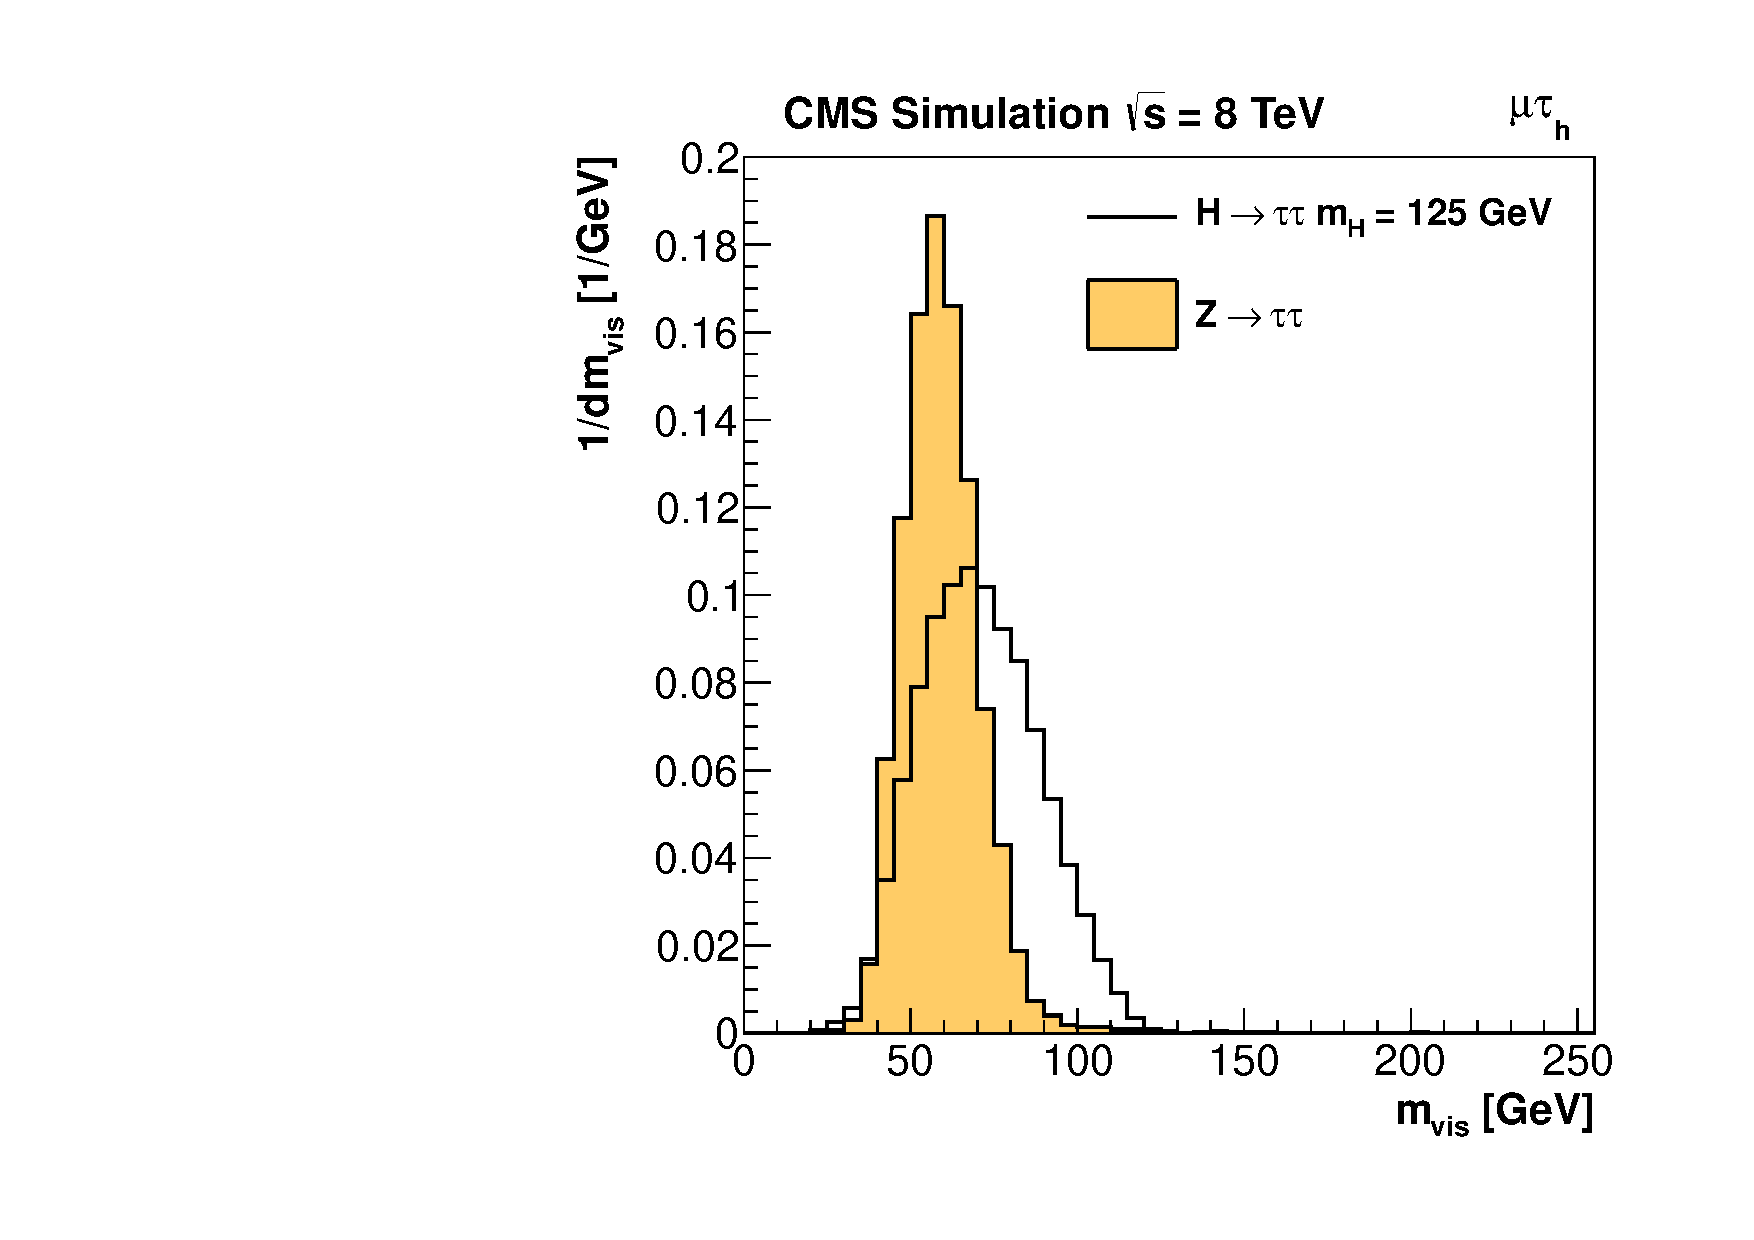
\includegraphics[width=0.5\textwidth]
      {plots/reco/svFitPerformance_forColin_visMass.pdf}}
\subfloat[]{
    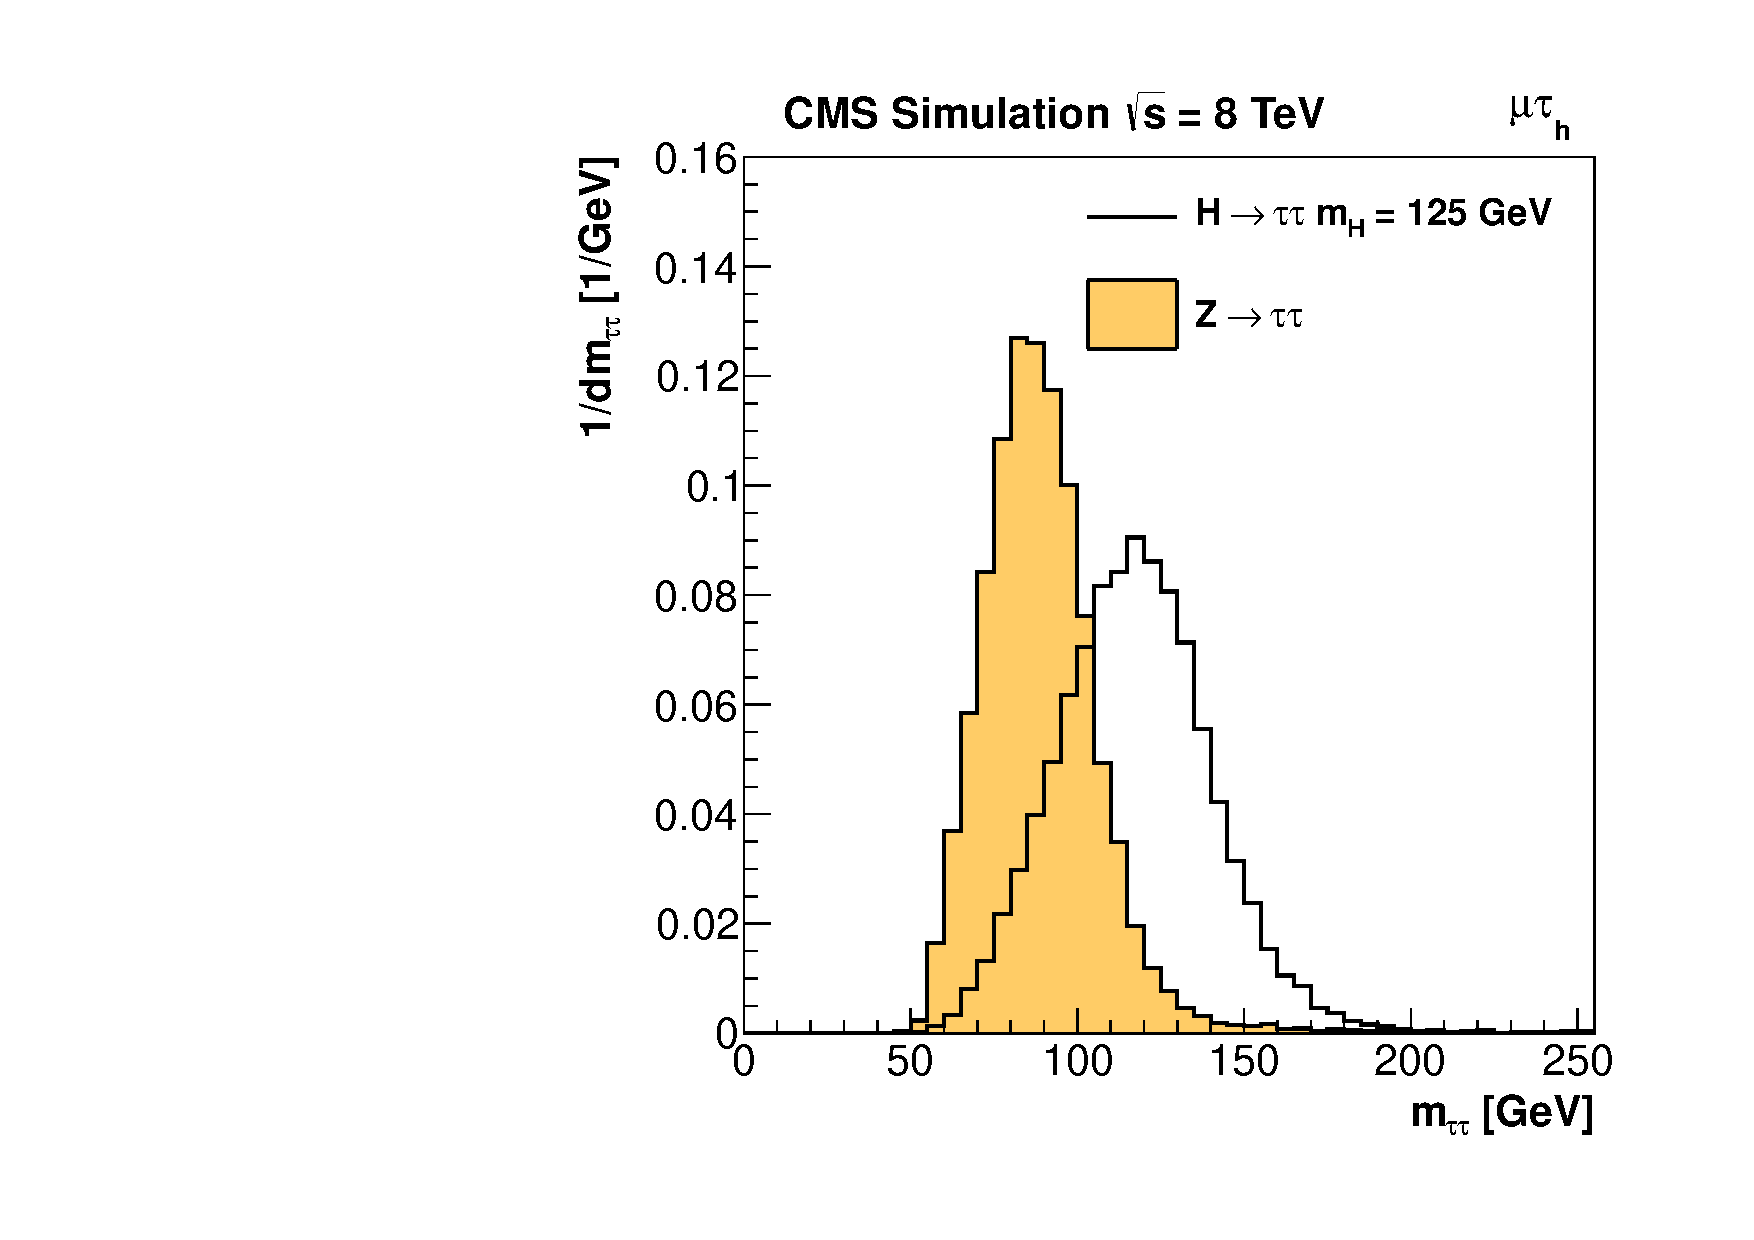
\includegraphics[width=0.5\textwidth] 
      {plots/reco/svFitPerformance_forColin_svFitMass.pdf}} 
\end{center}
\caption{
}
\label{fig:svfit}
\end{figure}

%\section{\ac{MC} simulation of signal and backgrounds}

%To model the contributions of signal and background events in the analysis
%Monte-Carlo (MC) simulation is used. Simulation of signal events is generated
%using POWHEG \cite{powheg} interfaced to PYTHIA \cite{pythia}, and of
%background events using MADGRAPH \cite{madgraph}. Pileup is simulated using
%additional interactions from PYTHIA and reweighting the simulated events to
%match the observed pileup distribution in data, which is different depending on
%the run period. In addition, the $E_{\rm{T}}^{\rm{miss}}$ response in
%simulation is corrected for the $E_{\rm{T}}^{\rm{miss}}$ energy scale and
%resolution which is measured in $Z\rightarrow\mu\mu$ events. The generated
%events are then processed through a simulation of the CMS detector based on
%GEANT4 \cite{geant4} and are reconstructed with the same algorithms used in
%data.




  \chapter{Search for Standard Model $\PH \to \Pgt\Pgt$}
\label{chap:httSM}

As described in chapter \ref{chap:theory}, the Higgs boson is the final missing 
piece of the Standard Model of particle physics. In order to complete the
\ac{SM}, this Higgs boson should have all the predicted properties of the
\ac{SM} Higgs, including decaying to tau leptons at the predicted rate. This
chapter describes the search for the Higgs boson of the Standard Model 
decaying into two tau leptons.

This chapter outlines the ``legacy'' result from run 1 of the \ac{LHC}, including the
full dataset collected in 2011 and 2012 by CMS. This corresponds to an
integrated luminosity of 4.9 fb$^{-1}$ at a centre of mass energy of 7 TeV and
19.7 fb$^{-1}$ at 8 TeV. The results in this chapter are parts of a publication 
in the Journal of High Energy Physics \cite{HIG-13-004}. The material included 
in this chapter is particularly focussed towards the parts of the analysis which 
included the work of the author. 

The $\PH \to \Pgt\Pgt$ analysis is performed in different final states dependent
on the final decay products of the taus. As discussed in section
\ref{sec:hadronictaus}, taus can decay into electrons $e$,
muons $\mu$ and hadrons (denoted $\tau_{h}$), all with associated neutrinos.
This gives a total of six possible final states, $\ee$, $\mumu$, $\emu$,
$\etau$, $\mutau$ and $\tautau$. The most direct involvement of the author in this
analysis and the analyses in the subsequent chapters was for the $\etau$ and
$\mutau$ channels, although considerable work was also done on the statistical
interpretation side using results from all channels. 
As such the analysis details described in sections \ref{sec:eventSelection},
\ref{sec:backgrounds}, \ref{sec:datamcfactors} and \ref{} are focussed on the
$\etau$ and $\mutau$ channels, whilst results including the combination of all
six channels, and additional channels from a dedicated $\PW\PH\to\Pgt\Pgt$ and
$\PZ\PH\to\Pgt\Pgt$ analysis, are shown in \ref{sec:results}. More detail on the other channels
can be found in \cite{HIG-13-004}. 

\section{Event Selection}
\label{sec:eventSelection}

This section describes how the objects described in chapter
\ref{chap:reco} are used to select the most signal-like events. 
The following sections describe in more detail the selections
used for each of the $\mutau$ and $\etau$ channels.

\subsection{Candidate Pair in the $\etau$ Channel}

Events in the $\etau$ channel require an electron and hadronic tau
candidate. The events are first selected by a trigger algorithm which requires
an electron and tau object. At the \ac{L1} trigger the requirement is simply a
single electron. Then at \ac{HLT} loose ID and isolation requirements are placed on the
electron, and additionally a $\tau_{h}$ object is required. For
this a simplified version of the \ac{PF} algorithm is used, and a loose
isolation is applied. These ID and isolation requirements are only approximate
compared to the more sophisticated algorithms which can be applied offline.  

In the offline selection the electron is required to have $\pt$ larger than ($20~\GeV$)
$24~\GeV$ in (2011) 2012 data. The higher $\pt$ cut in 2012 data is necessary
due to increased trigger thresholds necessary to maintain stable rates in the
higher instantaneous luminosity conditions. In all data taking periods the $\eta$ requirement
on the electron is $|\eta| < 2.1$. The electron is required to pass the electron
ID \ac{BDT} as described in section \ref{sec:electrons}, using a $\pt$ and
$\eta$ dependent cut which corresponds to the tight working point.  
The isolation definition described in section \ref{sec:leptonisolation} is
applied with a threshold of 0.1. The electron must be compatible with
originating at the chosen \ac{PV}, and so the impact parameters in the
transverse and beam directions, $d_{xy}$ and $d_{z}$ respectively, must be
small (less than ... ). 

The hadronic tau is selected with $\pt$ of larger than $30~\GeV$ and
$|\eta|<2.3$. The tau is identified using the \ac{HPS} algorithm as described in 
section \ref{sec:hps}. The tau must be compatible with
originating at the chosen \ac{PV}, and so the impact parameters in the
transverse and beam directions, $d_{xy}$ and $d_{z}$ respectively, must be
small (less than...). As described in section \ref{sec:tauleptonrejection}, 
tau candidates are required to pass criteria to reduce the mis-identification of electrons and
muons. In the $\etau$ channel, a tight working point for electron rejection is
used, and a loose working point for muon rejection. Isolation as described in
section \ref{sec:tauisolation} is applied using an optimised working point of
$1.5~\GeV$.  

The electron and hadronic tau are required to be of opposite charge. If more
than one such pair exists in the event, then the pair with the highest sum $\pt$
is selected. The $\pt$ and $\eta$ distributions of the selected pair in the
$\etau$ channel are shown in figure \ref{fig:etauelectrons} for the electron and
\ref{fig:etautaus} for the tau. 


\begin{figure}[htb]
\begin{center}
\subfloat[]{
    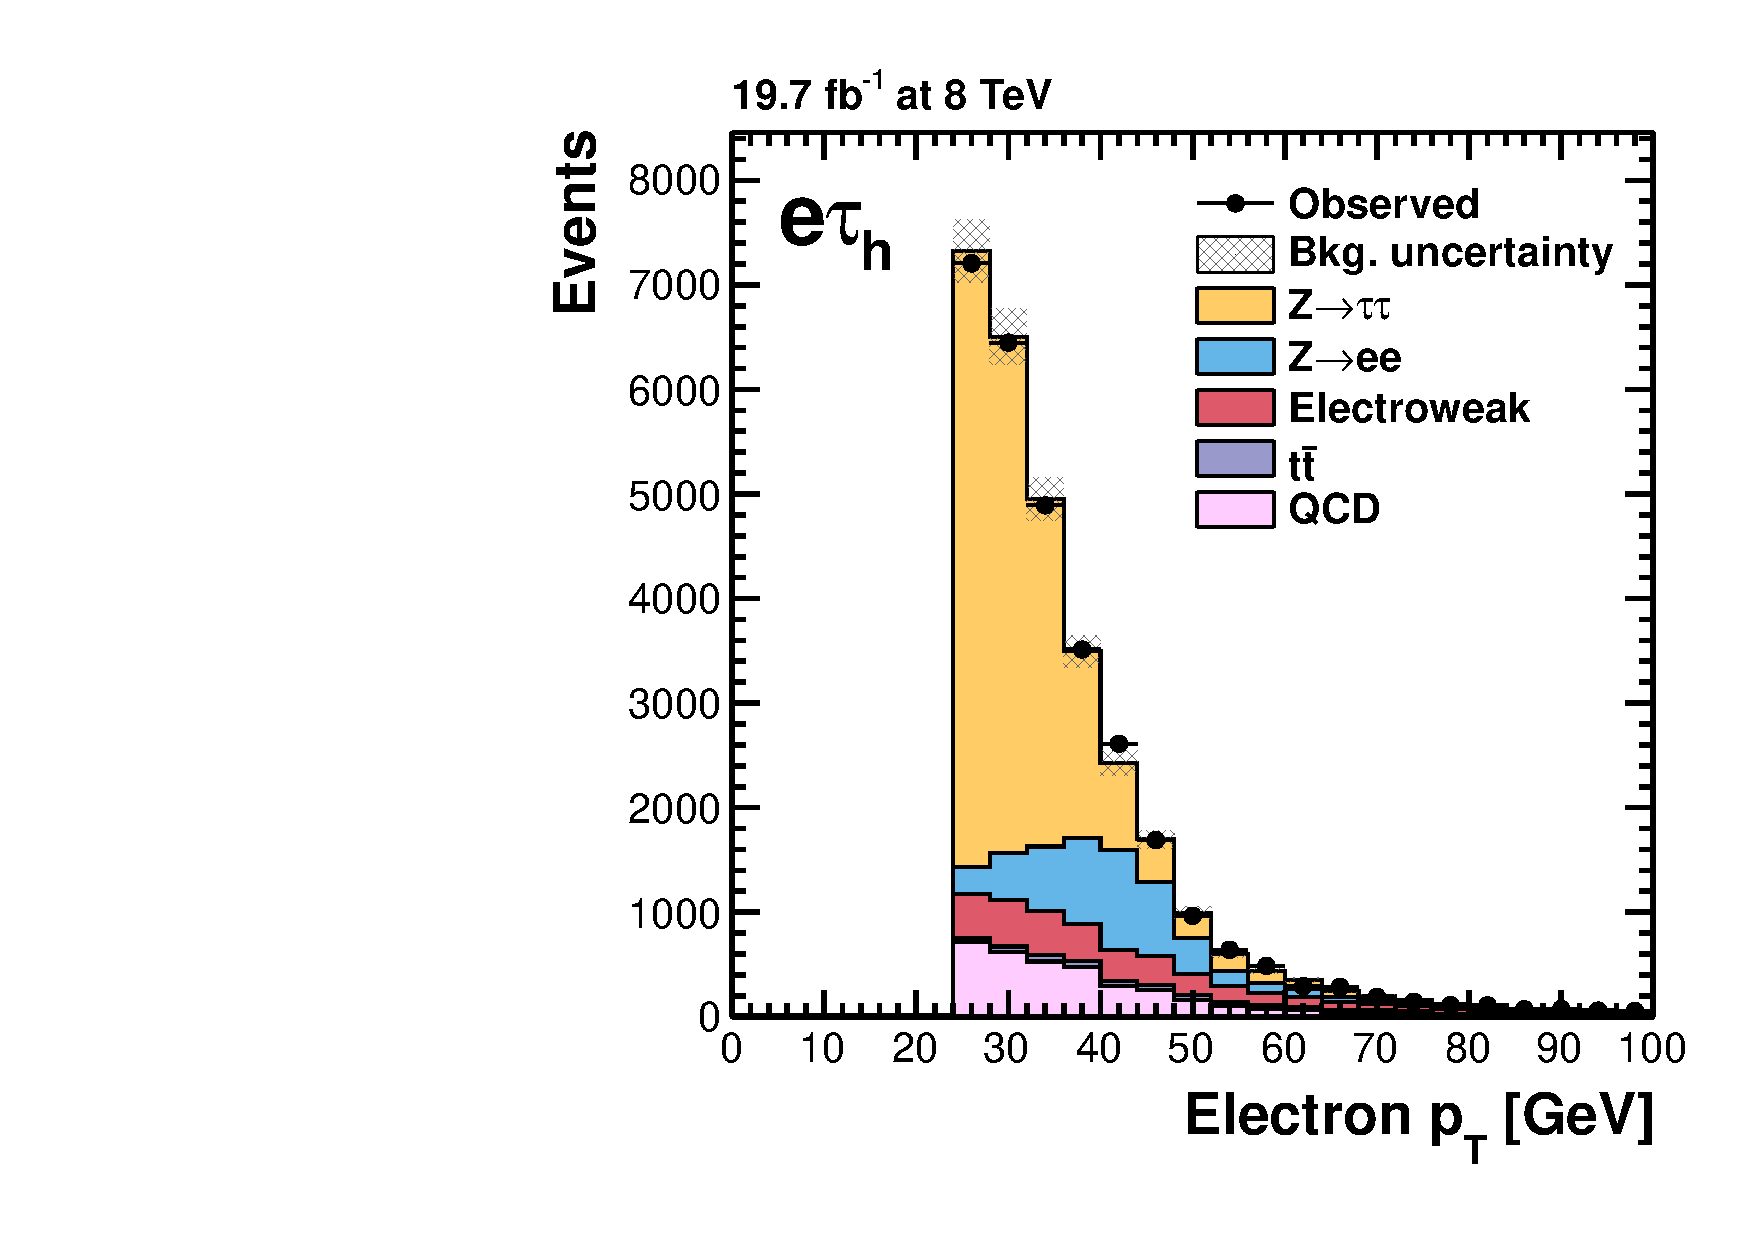
\includegraphics[width=0.5\textwidth]
      {plots/htt-sm/pt_1_inclusive_et_2012.pdf}}
\subfloat[]{
    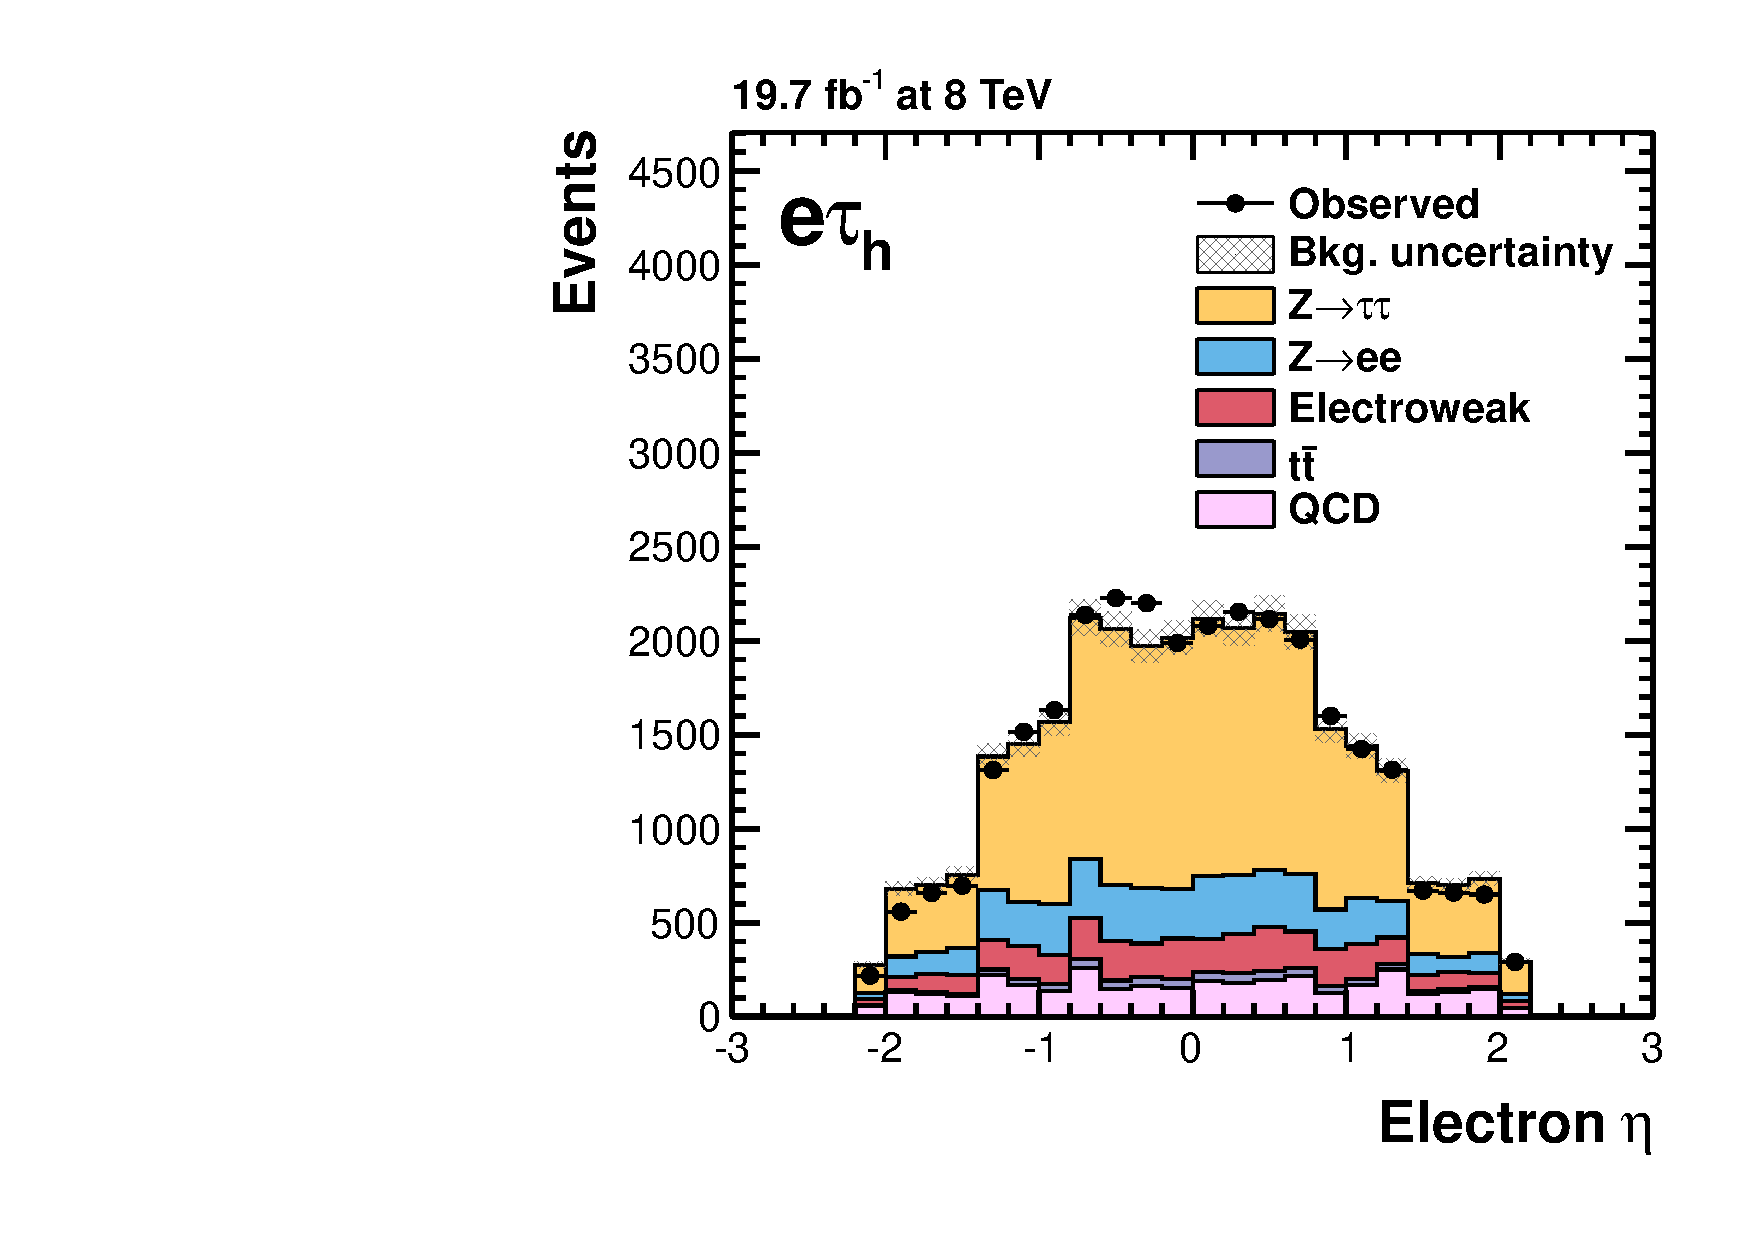
\includegraphics[width=0.5\textwidth] 
      {plots/htt-sm/eta_1_inclusive_et_2012.pdf}} 

\end{center}
\caption{
The $\pt$ and $\eta$ distribution for electron candidates in the $\etau$
channel.
}
\label{fig:etauelectrons}
\end{figure}


\begin{figure}[htb]
\begin{center}
\subfloat[]{
    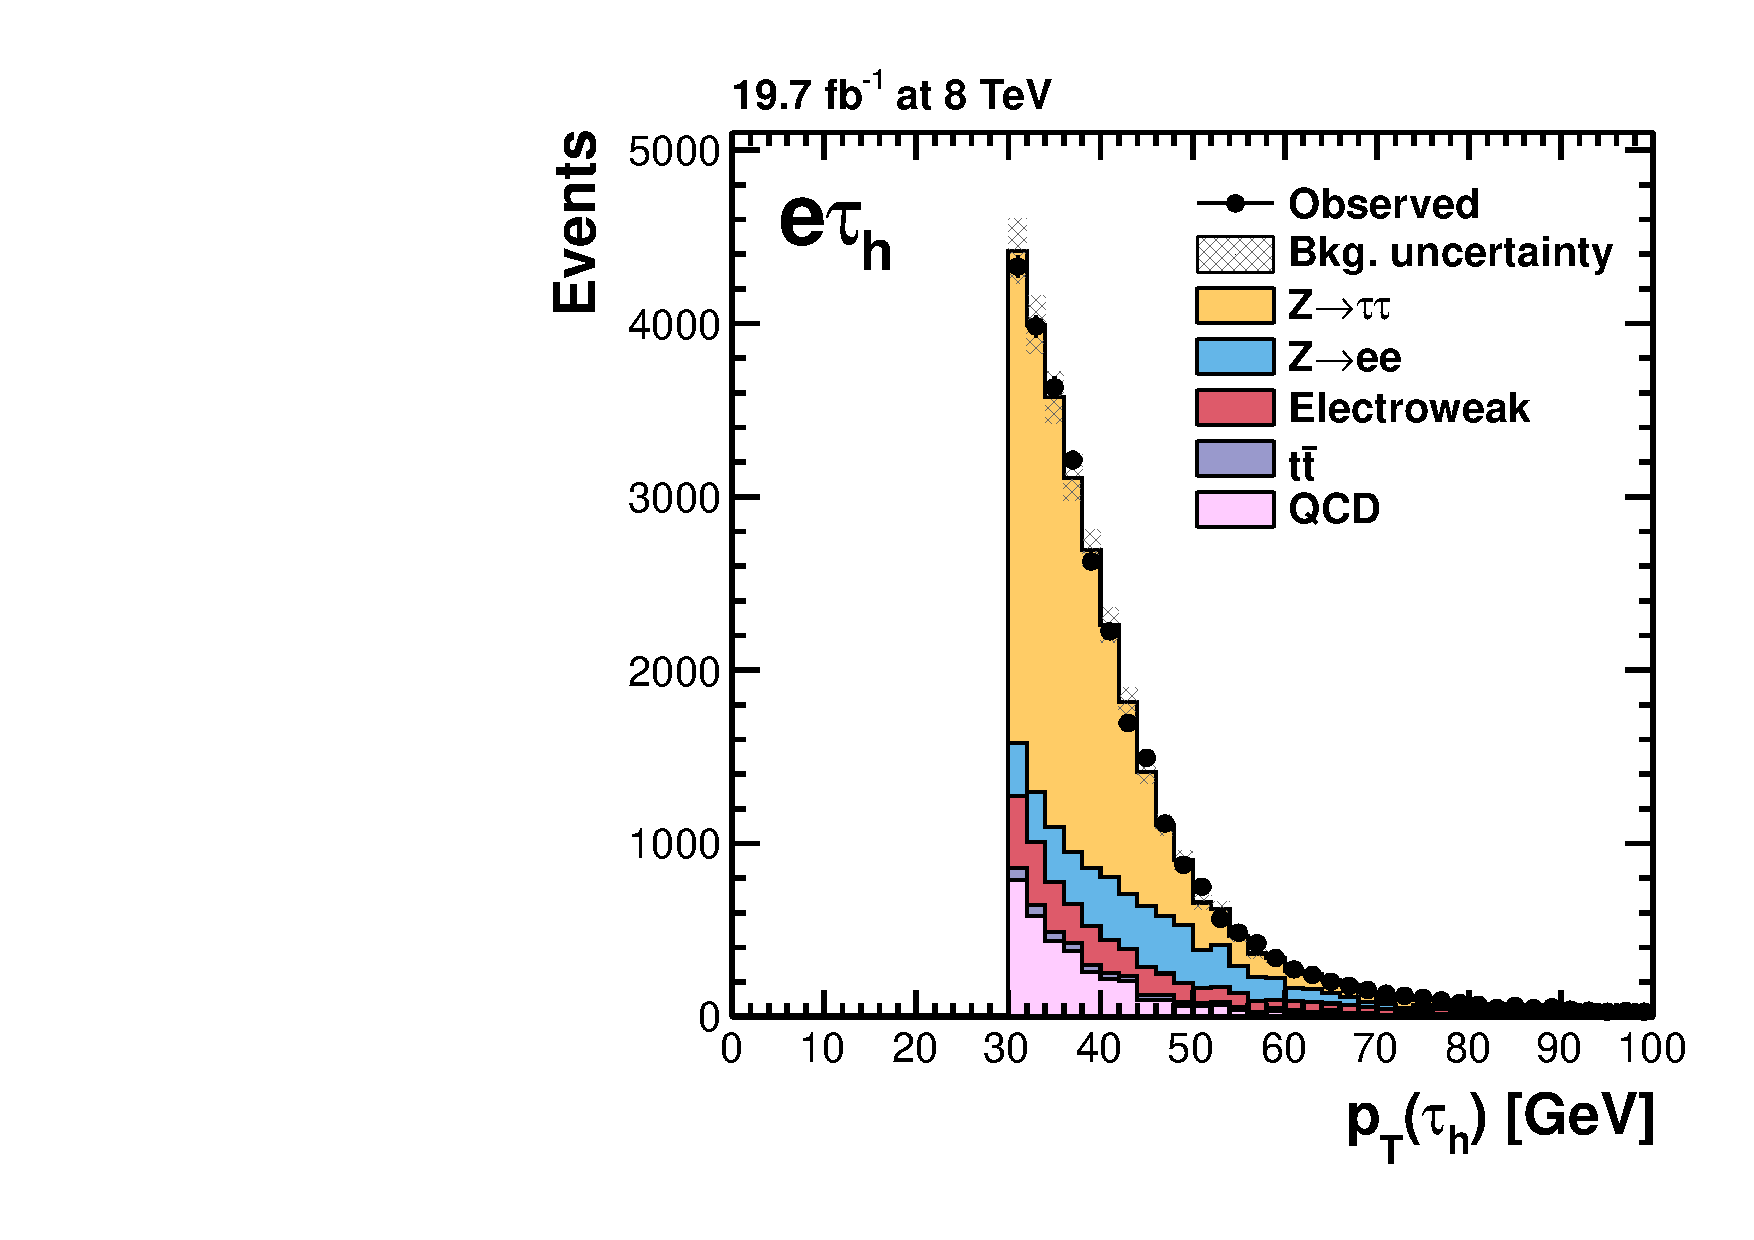
\includegraphics[width=0.5\textwidth]
      {plots/htt-sm/pt_2_inclusive_et_2012.pdf}}
\subfloat[]{
    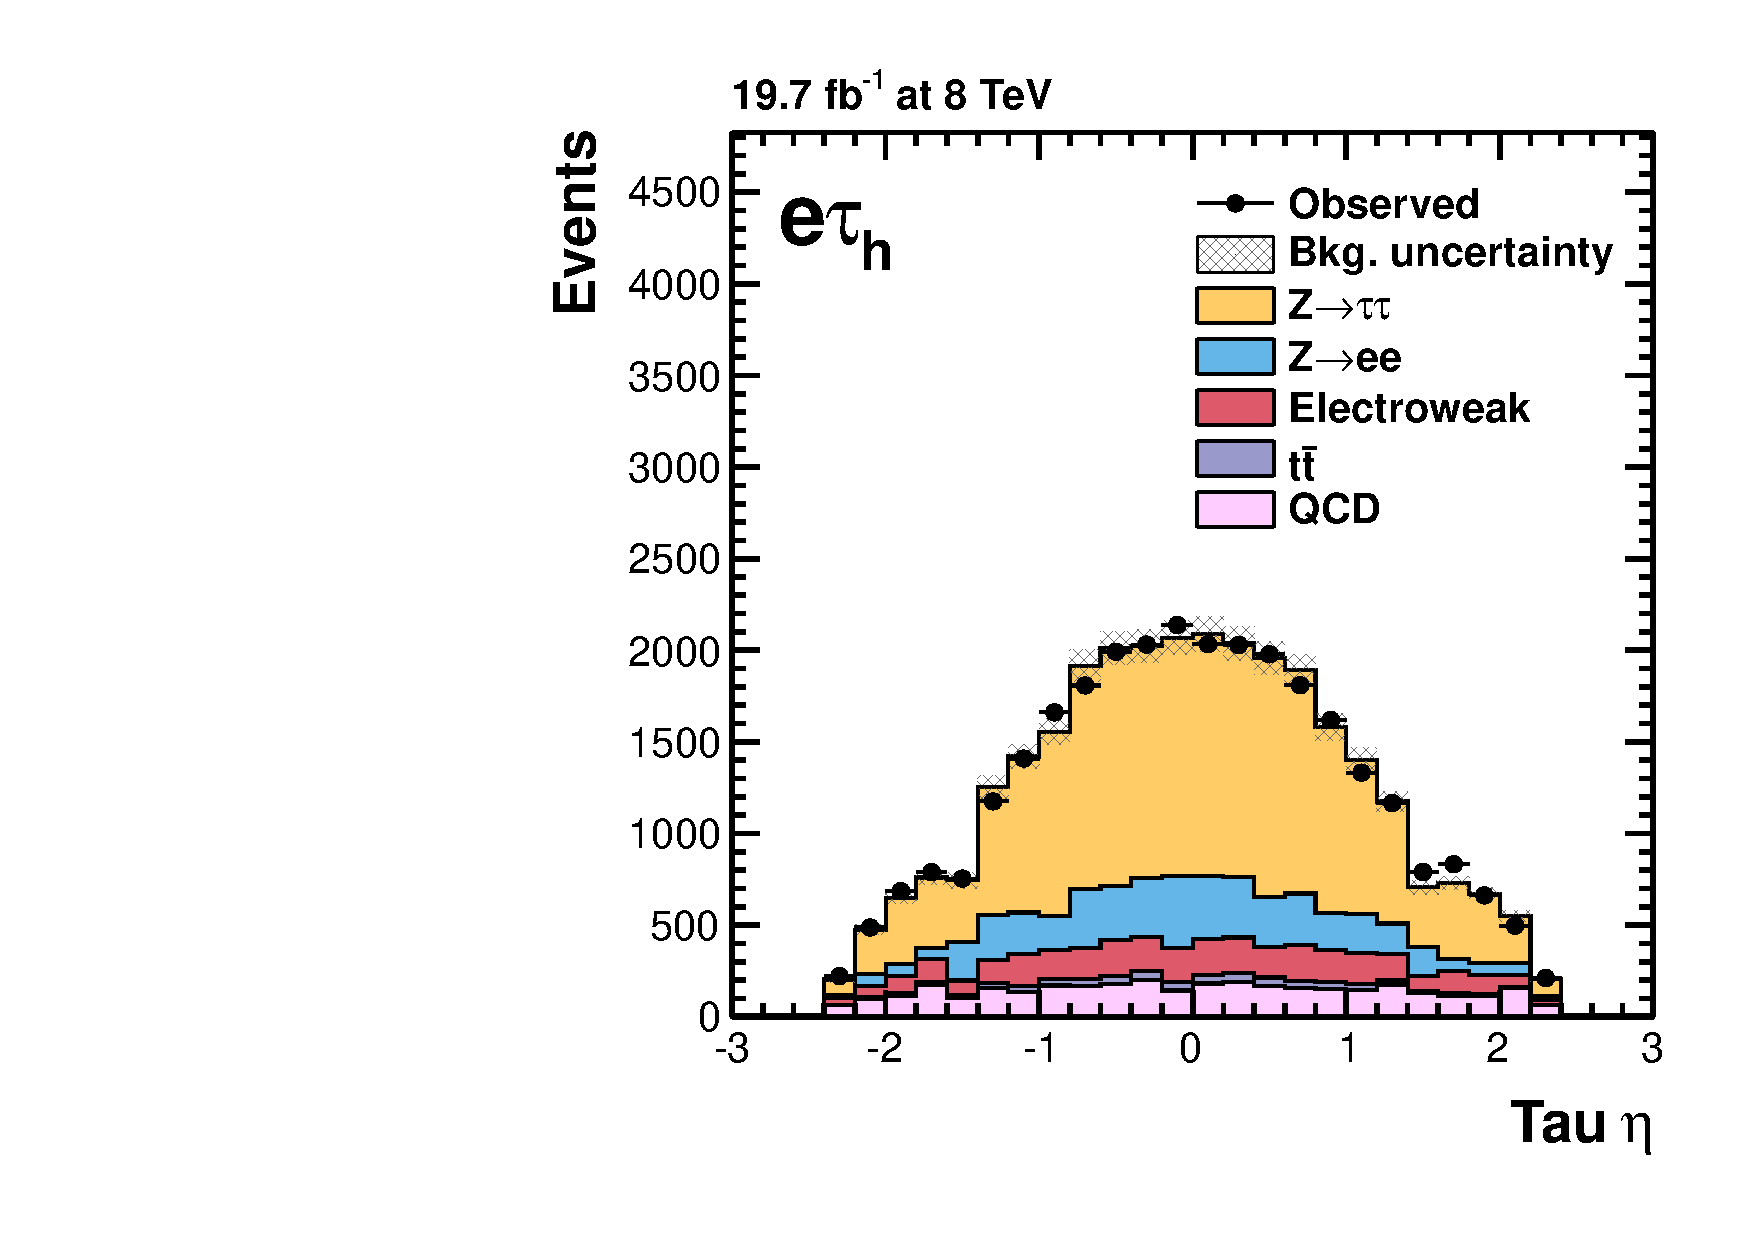
\includegraphics[width=0.5\textwidth] 
      {plots/htt-sm/eta_2_inclusive_et_2012.pdf}} 

\end{center}
\caption{
The $\pt$ and $\eta$ distribution for tau candidates in the $\etau$
channel.
}
\label{fig:etautaus}
\end{figure}

\subsection{Candidate Pair in the $\mutau$ Channel}

Events in the $\mutau$ channel require a muon and hadronic tau
candidate. The events are first selected by a trigger algorithm which requires
a muon and tau object. This is done in the same way as for the $\etau$ channel,
where the trigger object at \ac{L1} is a muon and the hadronic tau is
reconstructed at \ac{HLT} level.

In the offline selection the muon is required to have $\pt$ larger than ($17~\GeV$)
$20~\GeV$ in (2011) 2012 data. As for the $\etau$ channel, the higher $\pt$ cut is necessary for the
higher trigger threshold in 2012. In all data taking periods the $\eta$ requirement
on the muon is $|\eta| < 2.1$. The muon is required to pass tight muon ID as
defined in section \ref{sec:muons}. The isolation definition described in 
section \ref{sec:leptonisolation} is
applied with a threshold of 0.1. The muon must be compatible with
originating at the chosen \ac{PV}, and so the impact parameters in the
transverse and beam directions, $d_{xy}$ and $d_{z}$ respectively, must be
small. 

The hadronic tau has the same ID and isolation definition as described for the $\etau$
channel, with the exception of the anti-electron and anti-muon discriminators.
In the $\mutau$ channel a tight anti-muon discriminator and a loose
anti-electron discriminator are used. 

The muon and hadronic tau are required to be of opposite charge. If more
than one such pair exists in the event, then the pair with the highest sum $\pt$
is selected. The $\pt$ and $\eta$ distributions of the candidate pair in the
$\mutau$ channel are shown in figure \ref{fig:mutaumuons} for the muon and
\ref{fig:mutautaus} for the tau. 


\begin{figure}[htb]
\begin{center}
\subfloat[]{
    \includegraphics[width=0.5\textwidth]
      {plots/htt-sm/pt_1_inclusive_mt_2012.pdf}}
\subfloat[]{
    \includegraphics[width=0.5\textwidth] 
      {plots/htt-sm/eta_1_inclusive_mt_2012.pdf}} 

\end{center}
\caption{
The $\pt$ and $\eta$ distribution for muon candidates in the $\mutau$
channel.
}
\label{fig:mutaumuons}
\end{figure}


\begin{figure}[htb]
\begin{center}
\subfloat[]{
    \includegraphics[width=0.5\textwidth]
      {plots/htt-sm/pt_2_inclusive_mt_2012.pdf}}
\subfloat[]{
    \includegraphics[width=0.5\textwidth] 
      {plots/htt-sm/eta_2_inclusive_mt_2012.pdf}} 

\end{center}
\caption{
The $\pt$ and $\eta$ distribution for tau candidates in the $\mutau$
channel.
}
\label{fig:mutautaus}
\end{figure}

\subsection{Extra lepton vetos}

The contribution of certain backgrounds is reduced by vetoing events with extra
leptons in them. This is also crucial to ensure there is no event overlap
between categories, for example between the $\mutau$ channel and the
$\PW\PH\to\Pgt\Pgt$ analysis in the $\mu\mu\tau_{h}$ final state. In the
$\mutau$ and $\etau$ channels, events are vetoed if they contain an extra muon
or electron respectively, to reduce contribution from $\PZ\to\ell\ell$ in which
the $\tau_{h}$ is a fake from an extra misidentified jet in the event. In these
vetos, the definition of the extra lepton is slightly looser than the lepton ID
used for the candidate pair - with a $\pt$ requirement of $> 15~\GeV$ and
passing loose versions of the ID and isolation. A further veto on all events
containing any additional electron or muon candidate is applied, also with
relaxed selections. 

\subsection{Topological Selection}

After selection of the candidate pair, a large background from $\WJets$ remains
in the $\etau$ and $\mutau$ channels, usually with the lepton from the $\PW$ and
a jet faking the hadronic tau. A useful quantity to reduce this background is
the transverse mass between the lepton and the $\MET$:

\begin{equation}
m_{\text{T}}\equiv\sqrt{2\pt^{\ell}\MET(1-\cos(\Delta\phi))},
\end{equation}

where $\pt^{\ell}$ is the $\pt$ of the electron or muon and $\Delta\phi$ is the
difference in azimuthal angle between the lepton and the $\MET$. In real tau
events from $\PZ\to\Pgt\Pgt$ or $\PH\to\Pgt\Pgt$ the neutrinos in the $\Pgt$
decay tend to be produced collinearly with the visible products, whereas in
$\WJets$ events the neutrinos originate from the $\PW$ which has a much higher
mass than the $\Pgt$, and hence the neutrino is more likely to travel in the
opposite direction to the lepton in the transverse plane. Hence $\WJets$ events
have a higher transverse mass than signal events, and so a cut of
$m_{\text{T}}<30\,\GeV$ is found to reduce a large amount of $\WJets$ events
whilst still retaining a good signal efficiency.

Figure \ref{fig:transversemass} shows the distribution of $m_{\text{T}}$ for all
events in the $\mutau$ channel before the $m_{\text{T}}<30\,\GeV$ cut is
applied.

\begin{figure}[htb]
\begin{center}
    \includegraphics[width=0.5\textwidth]
      {plots/htt-sm/mt_1_inclusive_mt_2012.pdf}

\end{center}
\caption{
 The transverse mass between the muon and the $\MET$ in the $\mutau$ channel.  
}
\label{fig:transversemass}
\end{figure}


\section{Event Categorisation}
\label{sec:eventcategorisation}

The selection as described up until this point is referred to as the
``inclusive'' $\HToTauTau$ selection. 
Events with a good candidate lepton and tau pair are further categorised in
order to group events which are more background-like or signal-like. The
categorisation uses properties consistent with the different production modes of
the Higgs boson as described in section \ref{sec:theory}. Figure
\ref{fig:smcategories} illustrates these categories for the $\mutau$ and $\etau$
channels.

\begin{figure}[htb]
\begin{center}
    \includegraphics[width=0.8\textwidth]
      {plots/htt-sm/categories_2012.pdf}
\end{center}
\caption{
 Categories used in the $\etau$ and $\mutau$ channels of the \ac{SM}
 $\HToTauTau$ analysis \cite{HIG-13-004}.  
}
\label{fig:smcategories}
\end{figure}

The categorisation separates events which have 0,1 or 2 jets with $\pt>30~\GeV$
and $|\eta| < 4.7$. The jets are required to be separate from the lepton
candidates by $\Delta R > 0.5$. Events which contain a b-tagged jet as described in section
\ref{sec:btag} are vetoed to reduce the contribution of the $\ttbar$ background. 
The 0-jet categories are background dominant, and are included in the final
signal extraction to provide constraints on the backgrounds for the more signal
sensitive categories. The 1-jet categories are sensitive to gluon fusion Higgs
production in association with a jet and VBF Higgs production where one jet is
not picked up by the detector. The 2-jet categories are sensitive to
\ac{VBF} Higgs production, and the additional cuts on $m_{jj}$ and $\Delta
\eta_{jj}$ exploit the topology of this process. Events with additional jets in
the $\Delta \eta_{jj}$ gap are vetoed to reduce the \ac{QCD} background.

To improve sensitivity, categories are further separated into more signal-like
and background-like events. The 0-jet and 1-jet categories are separated by
$\tau_{h}$ $\pt$. The high $\pt^{\tau_{h}}$ events are more likely to be
consistent with a $\HToTauTau$ event than a $\ZToTauTau$ event due to the higher
mass of the Higgs than the $\PZ$. This also reduces contributions from \ac{QCD}
and $\WJets$ processes, where the jet faking the hadronic tau is likely to be
softer. An additional boosted category is used in 1-jet high $\pt^{\tau_{h}}$
events with a cut on the di-tau $\pt$, defined as:
\begin{equation}
\pt^{\Pgt\Pgt} = |\vec{\pt}^{L} + \vec{\pt}^{L'}+\vecMET|,
\end{equation}
with the requirement $\pt^{\Pgt\Pgt}>100~\GeV$. The VBF categories are split into VBF
``tight'' and ``loose'' based on tighter or looser $m_{jj}$ and
$\Delta\eta_{jj}$ cuts and the inclusion of the same ditau $\pt$ cut as in the
boosted 1-jet category. The distribution of the $\pt^{\Pgt\Pgt}$ in the
$\mutau$ channel is shown in figure \ref{fig:ditaupt}. 

\begin{figure}[htb]
\begin{center}
    \includegraphics[width=0.5\textwidth]
      {plots/htt-sm/pt_tt_inclusive_mt_2012_log.pdf}
\end{center}
\caption{
 Di-tau $\pt$ in the $\mutau$ channel as used for the separation of events into
 categories. 
}
\label{fig:ditaupt}
\end{figure}

The boosted 1-jet and the VBF tight categories are very 
signal sensitive, and also select events wth the best $m_{\tau\tau}$ resolution.
The VBF tight category is not possible in 2011 data due to the lower statistics,
so the VBF tight and VBF loose categories are merged. 

In the $\etau$ channel, 1-jet categories have an additional cut of $\MET >
30~\GeV$ to reduce the background from $\PZ\to\Pe\Pe$. This cut suppresses the
signal and $\ZToTauTau$ events with low $\pt^{\Pgt\Pgt}$, and as such the 1-jet low
$\pt^{\Pgt\Pgt}$ category is not possible in the $\etau$ channel.  

\section{Datasets and \ac{MC} samples}
\label{sec:dataandMC}

The data used in this analysis corresponds to that collected during the 2011 and
2012 running periods of the \ac{LHC}. Samples of background and signal events are produced using several different
\ac{MC} generators. The \textsc{madgraph}~\cite{Alwall:2011uj} matrix element
generator is used for the $\ZJets$, $\WJets$, diboson ($\PW\PW$, $\PZ\PZ$ and
$\PW\PZ$) and $\ttbar$ backgrounds. 
In order to have high enough statistics to evaluate the
backgrounds in the categories based on jet multiplicity, extra samples are
generated with fixed jet multiplicities up to 4 jets. These are combined with
inclusive samples using the expected ratio to retain the correct cross-section
ratios between jet multiplicity bins. The single top samples are generated using
\textsc{powheg}~\cite{Frixione:2007vw,Alioli:2010xd,Alioli:2010xa}, as are the
signal samples for gluon-fusion and \ac{VBF} at \ac{NLO} precision. Signal
samples for production in association with a vector boson are generated using
\textsc{pythia}~\cite{Sjostrand:2006za} at \ac{LO} precision only. In all
samples, \textsc{pythia} is used for parton showering and hadronisation and
\textsc{tauola}~\cite{TAUOLA} is used for tau decays. Minimum bias events
generated by \textsc{pythia} are added to all generated Monte Carlo samples
to simulate additional proton-proton interactions, and then the events are
weighted to match the pile-up profile observed in data. 

For the signal, \ac{MC} samples are produced in $5~\GeV$ steps between
$m_{H}=90~\GeV$ and $m_{H}=145~\GeV$. The cross-sections and branching ratios 
are taken from the \ac{LHCHXSWG}
\cite{LHCHiggsCrossSectionWorkingGroup:2011ti,Dittmaier:2012vm,Heinemeyer:2013tqia}.
The full set of simulated processes, the \ac{MC} generators used and the
cross-sections of the processes can be found in table \ref{tab:datasetsandMC}.

\begin{table}
\begin{tabular}{|l|c|c|c|}
\hline
Process & \ac{MC} Generator & \multicolumn{2}{c}{Cross Section [$\picobarn$]} \\
\cline{3-4}
&  & 7 \TeV & 8 \TeV \\
\hline
\hline
$\PW\to L\nu$ & \textsc{madgraph} & $31314$  & $36257$ \\
$\Pqt\Paqt$ & \textsc{madgraph}   & $164.4$   & $249.5$ \\
$\PZ\to LL$ & \textsc{madgraph}                      & $3048$    & $3504$ \\
$\PW\PZ\to \Pq\Pq'LL$ & \textsc{madgraph}          & $1.8$     & $2.2$ \\
$\PW\PZ\to L\Pnu LL$ & \textsc{madgraph}            & $0.9$     & $1.1$ \\
$\PZ\PZ\to LLLL$ & \textsc{madgraph}           & $0.06$    & $0.18$ \\
$\PZ\PZ\to LL\Pq\Pq$ & \textsc{madgraph}           & $0.8$     & $2.5$ \\
$\PZ\PZ\to LL\Pnu\Pnu$ & \textsc{madgraph}         & $0.3$     & $0.7$ \\
Single-top ($\Pqt\PW$ channel) & \textsc{powheg}            & $15.7$    & $22.2$ \\
\hline
SM $\Pg\Pg\PH(\Pgt\Pgt)$ & \textsc{powheg} & $0.96$ & $1.22$ \\
SM $\Pq\Pq\PH(\Pgt\Pgt)$ & \textsc{powheg} & $0.077$ & $0.010$ \\
SM $\PZ\PH(\Pgt\Pgt)$+$\PW\PH(\Pgt\Pgt)$+$\Pqt\Paqt\PH(\Pgt\Pgt)$ &
\textsc{pythia} & $0.063$ & $0.079$ \\
\hline
\end{tabular}
\caption{
Summary of the background and signal processes used in the $\HToTauTau$ analysis along with the
\ac{MC} generator and cross-section for the process in $7~\TeV$ and $8~\TeV$
conditions. The notation $L$ indicates a leptonic decay into $\Pe$, $\Pmu$ or
$\Pgt$, and $q$ indicates a quark. For the $\PW$, $\PZ$ and diboson backgrounds
samples are produced for jet multiplicities of 0, 1, 2, 3 and 4. The
cross-sections listed for the signal process are for $m_{H}=125~\GeV$.
}
\label{tab:datasetsandMC}
\end{table}

\section{Background Estimation}
\label{sec:backgrounds}

There are many backgrounds to $\HToTauTau$, and it is essential to estimate well
the contribution in each category. Where possible, data driven methods
are used to minimise systematic uncertainty related to the modelling in the
\ac{MC}. It is essential to accurately estimate both the shape and the overall
yield of each background.

\subsection{Drell-Yan $\PZ \to\Pgt\Pgt$}
\label{sec:backgroundEstimation_Ztautau}

The $\PZ \to \Pgt\Pgt$ component is the largest and is usually referred to as ``irreducible", due to its final
state involving two real taus which only differ from the $\PH \to \Pgt\Pgt$ signal by
having an invariant mass closer to the mass of the $\PZ$ instead of the Higgs.
The contribution from $\ZToTauTau$ in each category is estimated using an
``embedded'' sample. In this process a sample of $\PZ\to\Pmu\Pmu$ events are
collected and the muons replaced with simulated taus. These muons are required
to pass \ac{PF} identification and loose isolation and be of opposite charge.
The simulated taus are assigned the 4-momenta of the muons, and all other
quantities such as jets, $\MET$ and tau isolation are recomputed. The taus
are simulated by \textsc{tauola}. The $\ZToTauTau$ sample is used to esimate 
the inclusive yield of this background without the topological $m_{\text{T}}$
cut. 
The yield in each category is estimated by scaling this inclusive yield by the efficiency for 
inclusive events to pass the category selection, which is estimated using the
embedded sample. The shape is then taken from the embedded sample within the
category selection. The advantage of this is that the majority of event objects
are taken from data, and hence the systematic uncertainties related to $\MET$
and jet reconstruction are much smaller. 

%To account for the known contamination of $t \bar{t}$ events in the embedded
%samples, the embedded $t \bar{t}$ samples described in
%section~\ref{sec:datasets_and_MonteCarloSamples} are used to evaluate the
%expected contribution from such events, and then this is directly subtracted
%from the $\PZ \to\Pgt\Pgt$ contribution.

\subsection{$\PZ\to\ell\ell$}
\label{sec:backgroundEstimation_Zll}

The $\PZ\to\ell\ell$ background results when one lepton provides the electron or
muon and either the other lepton or an associated jet fakes the hadronic tau. This
background is much smaller than $\ZToTauTau$ but especially important in the
$\etau$ channel where electrons have a $3$-$4\%$ probability to pass the
anti-electron discrimination in the tau ID. Both yield and shape of this
background are taken from simulation.

\subsection{$\WJets$}
\label{sec:backgroundEstimation_WplusJets}

W plus jets is a background in this analysis where there is a real electron or
muon from the W and one of the associated jets fakes a hadronic tau. This
background is largely reduced by the $m_{\text{T}}< 30~\GeV$ cut described in
section~\ref{sec:eventSelection}. To estimate the remaining contribution the
events with $m_{\text{T}}> 70~\GeV$ are used, which are dominated by W+jets 
events. This is used to estimate the sideband normalisation of the W+jets, by
subtracting all other backgrounds from data and taking the rest to be W.
An extrapolation factor, to take the estimate from the high $m_{\text{T}}$ region to
give an estimate in the signal region with $m_{\text{T}}< 30~\GeV$, is calculated from MC.

The shape of the W is taken from MC in each category. Due to the low number of
events passing the VBF categories, the $m_{jj}$ and $|\Delta\eta_{jj}|$
conditions are relaxed in both calculating the extrapolation factor and
obtaining the shape.

\subsection{QCD}
\label{sec:backgroundEstimation_QCD}

QCD occurs when both the lepton and the tau are misidentified jets, and is estimated 
entirely from data. It is expected that the contribution of
same sign and opposite sign events from QCD is roughly the same. Thus the same
sign data is used with all other backgrounds subtracted, to predict the rate of
QCD in the opposite sign events. For the background subtraction, the W+jets is
estimated as described in the previous section and all other background
contributions are estimated from MC. The opposite sign/same sign rates from QCD
are not quite exactly the same, and an extrapolation factor of 1.06, measured
using data with the electron/muon isolation inverted, is applied to correct for
this. This is the method for extracting the norm in all of the 0-jet and 1-jet
categories, with the exception of 1-jet high-$\pT^{\Pgth}$ boosted.

Due to the low statistics in the 1-jet high-$\pT^{\Pgth}$ boosted and the VBF
categories, it is necessary to define another
sideband from which to extract the QCD estimate. This is done by inverting the
electron/muon isolation to $0.2<R^{\Pe/\Pgm}<0.5$ in same-sign events. The
inclusive same-sign yield is taken from the normal isolation region, and scaled
by the efficiency to go from the inclusive to the category selection as
estimated in the anti-isolated data. 

In the 0-jet low-$\pT^{\Pgth}$ category the shape is taken from the normal
isolated same-sign data with other backgrounds subtracted. In all other
categories the anti-isolated data is used for the shapes. The high purity for
QCD multijet events in anti-isolated same sign data makes it unnecessary to
subtract other backgrounds, which are negligible. In the 1-jet
high-$\pT^{\Pgth}$ boosted and tight VBF-tag categories the isolation on the
$\Pgt_{had}$ is also loosened to obtain a sufficiently smooth shape.  

\subsection{$\ttbar$}
\label{sec:backgroundEstimation_TT}

For the $t \bar{t}$ both shape and normalisation are taken from MC. Both are checked
against data by defining a control region which is at least 90$\%$ pure in
$t \bar{t}$. This is done using the $\emu$ channel, which has a much higher
quantity of $\ttbar$ than $\etau$ and $\mutau$. The control region is used to
derive a scale factor to the \ac{MC} normalisation. 

\subsection{Diboson and single top}
Both the normalisation and shapes of these backgrounds are estimated using MC.
The contributions from these backgrounds are much smaller than the others.

\section{Data/MC Correction Factors}
\label{sec:datamcfactors}

Whilst data-driven methods are used wherever possible, MC is still
relied on in predicting expected shapes and yields of signal and backgrounds.
As such is it important that the MC is corrected for
any effects which are known to be imperfectly modeled. Many of these corrections
are derived by studying the agreement between \ac{MC} and data in dedicated
samples or control regions.

\subsection{ID, isolation and trigger efficiencies}

For ID, isolation and trigger efficiencies of the candidate electron/muon 
and tau in the analysis, the \ac{MC} is corrected for measured differences in 
the efficiency in data and \ac{MC}.

This section documents measurements of these efficiences for the electron/muon 
of the $\etau$ and $\mutau$ channels. This is done using a ``tag and probe"
method \cite{Khachatryan:2010xn}.
The tag and probe method makes use of a well known and measured resonance decaying
into a light lepton pair, in this case $\PZ\to\Pe\Pe$ or $\PZ\to\Pmu\Pmu$, 
in which one the light leptons is assigned as the `tag' and one is the `probe'. 
The tag is constrained by a very tight selection such that it is known with near 
certainty to be a real electron/muon. The probe is subject to a looser selection, 
but only tag/probe pairs with an invariant mass close to the $\PZ$ mass are used. 
This ensures that the probe is also a true electron/muon with high probabiliy. 
Then the probe can be subjected to further cuts or constraints to measure the 
efficiency of such a selection to select real leptons.

The invariant mass distributions of the tag and probe events are used to extract
the different selection efficiencies. A simultaneous fit of the passing and failing probe 
mass shapes is performed, and the ratio of the integral of the fitted $\PZ$ signal 
in the pass and fail distributions is used to extract the efficiency. To account for any background
to the real $\PZ$ events, signal and background are both accounted for
separately in the fit. An example of such a fit can be seen in figure
\ref{fig:tandp}.

The electron/muon ID efficiency is measured with a reconstructed
electron/muon as the probe, subject only to $\pt$ and $\eta$ cuts. 
Then the electron/muon isolation efficiency is measured
with a probe which already fulfils the full ID selection criteria. 

The efficiencies for combined ID and isolation are shown in Figures
\ref{fig:electronIdIso} and \ref{fig:muonIdIso}, measured in the complete 2012
dataset and PU weighted MC, as a function of the lepton $\eta$ and $\pt$.
The scale factor which is used in the analysis is given by the ratio of the
measured efficiency in data (black) and MC (red), and is evaluated separately in
selected $\pt$ and $\eta$ bins.

\begin{figure}[htb]
\subfloat[]{
\includegraphics[width=0.5\textwidth]{plots/TagAndProbe/ElectronIdIsoEta2012DatavsMC.pdf}}
\subfloat[]{
\includegraphics[width=0.5\textwidth]{plots/TagAndProbe/ElectronIdIsoPT2012DatavsMC.pdf}}
\caption{Combined electron ID and isolation efficiency in data and MC as a
function of (left) $\eta$ and (right) $\pt$}
\label{fig:electronIdIso}
\end{figure}

\begin{figure}[htb]
\subfloat[]{
\includegraphics[width=0.5\textwidth]{plots/TagAndProbe/MuonIdIsoEta2012DatavsMC.pdf}}
\subfloat[]{
\includegraphics[width=0.5\textwidth]{plots/TagAndProbe/MuonIdIsoPT2012DatavsMC.pdf}}
\caption{Combined muon ID and isolation efficiency in data and MC as a function
of (left) $\eta$ and (right) $\pt$}
\label{fig:muonIdIso}
\end{figure}

The same method is used to measure the efficiencies of the trigger
in data and MC. In this case a probe is used which has already passed both ID
and isolation, and the passing probe condition is that the lepton is responsible
for firing the lepton leg of the lepton plus tau trigger. Figures
\ref{fig:electrontrg} and \ref{fig:muontrg} show the trigger efficiency as a
function of $\pt$ measured in both 2012 data and MC. For the
electrons, the trigger is measured separately in the barrel and endcap
regions, which correspond to $|\eta| < 1.479$ and $|\eta| > 1.479$
respectively. For the muons, the trigger is measured in 3 regions, corresponding
to the different regions of the muon chambers.

\begin{figure}[htb]
\subfloat[]{
\includegraphics[width=0.5\textwidth]{plots/TagAndProbe/ee_TP_fit.pdf}}
\subfloat[]{
\includegraphics[width=0.5\textwidth]{plots/TagAndProbe/ee_TF_fit.pdf}}
\caption{Fitted $m_{ee}$ peaks for $\PZ\to\Pe\Pe$ tag and probe data events with a probe passing (a) and
failing (b) matching to the electron leg of the $\etau$ trigger. This example
fit is for electrons with $26 <\pt< 30~\GeV$ in the barrel. A separate function is fitted for the
background and signal ($\PZ\to\Pe\Pe$) contributions. The ratio of the integrals
of these two fits gives the trigger efficiency of the electrons, which is
approximately $80\%$ for this $\pt$ and $\eta$ range.}
\label{fig:tandp}
\end{figure}


\begin{figure}[htb]
\subfloat[]{
\includegraphics[width=0.5\textwidth]{plots/TagAndProbe/ElectronBarrel2012DatavsMC.pdf}}
\subfloat[]{
\includegraphics[width=0.5\textwidth]{plots/TagAndProbe/ElectronEndcap2012DatavsMC.pdf}}
\caption{Efficiency of the electron leg of the $\etau$ trigger as a function of electron $\pt$ measured
in 2012 data and MC in the (left) barrel and (right) endcaps.}
\label{fig:electrontrg}
\end{figure}

\begin{figure}[htb]
\subfloat[]{
\includegraphics[width=0.5\textwidth]{plots/TagAndProbe/MuonAbsEta082012DatavsMC.pdf}}
\subfloat[]{
\includegraphics[width=0.5\textwidth]{plots/TagAndProbe/MuonAbsEta122012DatavsMC.pdf}}

\begin{center}
\subfloat[]{
\includegraphics[width=0.5\textwidth]{plots/TagAndProbe/MuonAbsEndcap2012DatavsMC.pdf}}
\end{center}
\caption{Efficiency of the muon leg of the $\mutau$ trigger as a function of muon $\pt$ measured in
2012 data and MC in the region (top left) $|\eta|$ $<$ 0.8, (top right) 0.8
$<$ $|\eta|$ $<$ 1.2 and (bottom) $|\eta|$ $>$ 1.2.}
\label{fig:muontrg}
\end{figure}

\subsection{Other corrections}

An additional correction is applied in the \ac{SM} gluon-gluon fusion signal
samples to exploit recent improved predictions. Events are weighted to match the
Higgs boson $\pT$ distribution calculated at \ac{NNLO} using the
\textsc{HRes}~\cite{deFlorian:2012mx} program. This also includes the
resummation at \ac{NNLL} accuracy of terms of the form
$\ln(m_{\PH}^{2}/\pT^{2})$ which are particularly important for low Higgs boson
$\pT$. An event weight for the difference between the finite and infinite top
mass approximations is also applied \cite{Grazzini:2013mca}.
A reweighting is applied to $t \bar{t}$ events. The correction has been developed by the Top
group to better match the top quark $P_{T}$ distribution observed in data~\cite{TopPtReweighting}. 
The contribution of $Z/\gamma^{*} \to ee$ background to the $e\tau_{had}$ channel
is additionally corrected by $e \to \tau_{had}$ fake--rate Monte Carlo--to--data
scale--factors

b-tag scale factors - add equation.

\section{Systematics}
\label{sec:systematics}

The systematic uncertainties consist of two different types:

\begin{itemize} 
\item Normalisation uncertainties: these affect the yield of a particular background or
signal.
\item Shape uncertainties: these affect the shape of the signal or background, or in
other words the number of signal or background events in a particular bin rather
than the overall number.
\end{itemize}

The way in which these different types of uncertainties are incorporated in the
final results is described in section \ref{sec:signalextraction}. The different
sources of uncertainties and their chosen values is described in the next
section separately for the normalisation and shape uncertainties.

\subsection{Normalisation Uncertainties}
\label{sec:systematicUncertainties_yield}

The uncertainties in the analysis which contribute to the normalisation of the
background or signal processes are as follows:

\begin{itemize}
\item \textbf{ID, isolation and trigger efficiencies for the electrons, muons and
hadronic taus}.\\
Data to MC scale factors as described in \cite{CMS_AN_2013-171}
are measured for this analysis and applied to correct for differences in these
efficiencies in MC compared with data. The estimated uncertainty in these
measurements are combined in quadrature. For the electrons and muons, this
amounts to a 2$\%$ normalisation uncertainty, which is applied to all
backgrounds in which the yield is taken from MC and signal.
For the hadronic taus a 6$\%$ uncertainty
is measured on the tau identification efficiency using 
$Z/\gamma^{*} \to \tau\tau \to \mu\tau_{had}$
events~\cite{TauIDRecommendation}. For the hadronic tau leg of the trigger, the
uncertainty is 3.0$\%$ for the triggers of the $e\tau_{had}$ and $\mu\tau_{had}$
channels and 4.5$\%$ for each leg of the trigger in the $\tau_{had}\tau_{had}$
channels. These uncertainties are applied to all backgrounds in which the yield
is taken from MC and signal.
\item \textbf{$e \to \tau_{had}$ and $\mu \to \tau_{had}$ fake--rates} \\
The uncertainty on the $e \to \tau_{had}$ fakerate is determined as part of
its measurement, and a description can be found in \cite{CMS_AN_2013-171}.
This amounts to an uncertainty of $30\%$, correlated between $\tau_{had}$ candidates
reconstructed in any tau decay mode. The uncertainty on the rate of $\mu \to \tau_{had}$
fakes is taken from the Tau POG~\cite{TauIDRecommendation}, amounting to $30\%$. 
\item \textbf{b--tag scale--factors} \\
Uncertainties on b--tagging efficiencies and mistag rates as function of jet
$P_{T}$ and $\eta$ for a particular b-tag working point of the CSV discriminator
(in the case of this analysis the medium working point) are provided by the BTV 
POG~\cite{BTagSFRecommendation}. The effect of these uncertainties on the
analysis is evaluated by varying the scale factors applied within their
recommended uncertiainties and evaluating the overall change in yield as a
result in each channel and category for each background. For those backgrounds
with a non-negligible variation as a result of this uncertainty the yield change
is applied as a normalisation uncertainty.
\item \textbf{$Z$--recoil correction} \\
Uncertainties on \MET resolution and response are accounted for
by varying the $Z$--recoil correction parameters within the uncertainties determined within the method.
\MET and all \MET related observables (including $M_{\tau\tau}$) are recomputed after each such variation.
\item \textbf{Background Normalisation} \\
The normalisation uncertainties on the backgrounds are evaluated where possible
by using alternative methods for estimation and studying the difference in yield,
and/or an uncertainty is applied which covers the statistical uncertainty on the
yield prediction from the default method. 

The normalization of the $Z/\gamma^{*} \to \tau\tau$ embedded samples in the inclusive event
category, obtained using Monte Carlo samples as described in
section~\ref{sec:backgroundEstimation_Ztautau}, is attributed an uncertainty of
$3\%$. The uncertainty as a result of extrapolation from the inclusive selection
to the category selection is 5$\%$ in the 2jet--0tag and 2jet--1tag categories,
and 6$\%$ in the 2jet--2tag category. An additional uncertainty on the $Z/\gamma^{*} \to \tau\tau$ 
is included to account for the subtraction of
the $t \bar{t}$ contamination in the embedded samples, where the size of the
uncertainty is equal to the size of the contamination. 

The $Z/\gamma^{*} \to \ell\ell$ ($\ell = e$, $\mu$) background is very small
after the requirement of 2 jets, and so the dominant uncertainty is from the
statistical uncertainty on the yield estimate. This uncertainty is estimated separately
for the components where it is either a jet or a lepton which fakes the hadronic 
tau. The uncertainty on the jet component is 20$\%$ (20$\%$) in the 2jet--0tag,
20$\%$ (25$\%$) int the 2jet--1tag and 90$\%$ (70$\%$) in the 2jet--2tag
category in the $\mu\tau_{had}$ and $e\tau_{had}$ channels respectively.
The corresponding uncertainties on the leptonic component
are 30$\%$ (20$\%$) in 2jet--0tag, 60$\%$ (20$\%$) in 2jet--1tag and 60$\%$
(40$\%$) in 2jet--2tag. 

The uncertainty on the $t \bar{t}$ cross-section amounts to $10\%$, and on the single top and di--boson
production cross--sections amounts to $15\%$.

The normalization of the $W$ + jets background is obtained from data, 
using the high $M_{T}$ sideband extrapolation method described in
section~\ref{sec:backgroundEstimation_WplusJets}. The uncertainty on the W
estimate is dominated by the data statistics available in this control region, and
amounts to 10$\%$ in the 2jet--0tag category, 40$\%$ in the 2jet--1tag category
and 100$\%$ in the 2jet-2tag category. 

The uncertainty on the normalization of QCD background is obtained by adding the
statistical uncertainty on the yield of events selected in the QCD dominated control regions
described in section~\ref{sec:backgroundEstimation_QCD} in quadrature with the
uncertainty on opposite sign - same sign factor of 1.06, which is around 10$\%$. 

%\item \textbf{Theoretical Uncertainties} \\
\item \textbf{Luminosity} \\
  The uncertainty on the luminosity amounts to $2.6\%$ for $2012$ data.
  This uncertainty is applied to the signal
  and to $Z/\gamma^{*} \to \ell\ell$ ($\ell = e$, $\mu$), $Z/\gamma^{*} \to
  \tau\tau$, $t \bar{t}$, single top and di--boson backgrounds. 
  The normalization of the $W$ + jets and QCD backgrounds is obtained from data and hence not subject to the luminosity uncertainty.
\end{itemize}

\subsection{Shape Uncertainties}
\label{sec:systematicUncertainties_yield}

\begin{itemize}

\item \textbf{$\tau_{had}$ energy scale} \\
When studying mass distributions, the shape of the distribution is directly
dependent on the energy scale of the objects making up the mass. Thus the
$m_{\tau\tau}$ and 4 body mass shapes are sensitive to the tau energy scale.
To incorporate this uncertainty, the energy scale of hadronically decaying taus is varied by $3\%$,
following the recommendation of the Tau POG~\cite{TauIDRecommendation}. 
in the previous section.
\item \textbf{$Z \to \ell\ell$ lepton energy scale}\\
A shape uncertainty is also added for the $Z \to \ell\ell$ contribution for the
events in the $e\tau_{had}$ and $\mu\tau_{had}$ channels where a lepton fakes a
hadronic tau, to account for the effect of the energy scale of the lepton fake.
This energy scale mismeasurement is estimated to give a shift of up to 2$\%$ in the
mass shape of the contribution, and hence a shape systematic amounting to the
2$\%$ shift up and down is included to cover for this effect.

\end{itemize}

\section{Results}
\label{sec:results}

\subsection{Signal Extraction}
\label{sec:signalextraction}

\subsection{Limit and Significance}
\label{sec:significance}

\begin{figure}[h!]
\subfloat[]{
\includegraphics[width=0.5\textwidth]{plots/htt-sm/cmb_limit.pdf}}
\subfloat[]{
\includegraphics[width=0.5\textwidth]{plots/htt-sm/cmb_limit_signalinjected.pdf}}
\caption{Expected and observed limit}
\label{fig:results-limit}
\end{figure}

\begin{figure}[h!]
\includegraphics[width=0.5\textwidth]{plots/htt-sm/cmb_p-value.pdf}
\caption{P value}
\label{fig:results-limit}
\end{figure}


\subsection{Consistency with $125~\GeV$ Higgs}
\label{sec:consistency}

\begin{figure}[h!]
\subfloat[]{
\includegraphics[width=0.5\textwidth]{plots/htt-sm/cmb-mass_scan.pdf}}
\subfloat[]{
\includegraphics[width=0.5\textwidth]{plots/htt-sm/cmb-scan-hww-CV-CF-125.pdf}}
\caption{Mass scan and couplings}
\label{fig:results-properties}
\end{figure}


  \chapter{Search for \ac{MSSM} $\Pphi\to\Pgt\Pgt$}
\label{chap:httmssm}

As discussed in chapter \ref{chap:theory}, from the \ac{LHC} we have observation
of a $125~\GeV$ Higgs boson which is so far consistent with the \ac{SM}. From
chapter \ref{chap:htt-sm}, we have evidence at the $3\sigma$ level of a Higgs
boson decaying into tau leptons, which has properties consistent with the $125~\GeV$ boson
discovered in the other decay channels and consistent with the \ac{SM}.
However, as discussed in section \ref{sec:mssmhiggs}, the \ac{MSSM} is an
alternative theory to the \ac{SM} which could provide a $125~\GeV$ Higgs boson
consistent with the properties observed so far experimentally. In this theory,
we would also see two additional neutral Higgs bosons. This chapter describes
the search for the three neutral Higgs bosons of the \ac{MSSM} in the final
state of $\Pgt\Pgt$. We use the symbol $\Pphi$ to refer to any one of the three
neutral Higgs bosons, $\PH$, $\Ph$ or $\PA$. This analysis largely uses the same
techniques as the \ac{SM} $\HToTauTau$ analysis and as such this chapter focusses on the
places that the analysis is different and on the interpretation of results in
the context of the \ac{MSSM}. The results documented are the ``legacy''
\ac{MSSM} $\Pphi\to\Pgt\Pgt$ result from run 1 of the \ac{LHC} \cite{HIG-13-021}, and like for
chapter~\ref{chap:htt-sm} the information is focussed on the analysis in the
$\etau$ and $\mutau$ final states. The results shown in
section~\ref{sec:mssmresults} include the combination of all channels, which for
the \ac{MSSM} analysis includes the $\etau$, $\mutau$, $\emu$, $\tautau$ and
$\mumu$ final states. 

\section{Event Selection and Categorisation}
\label{sec:mssmEventSelection}

The inclusive selection of the candidate di-tau pair is almost exactly the same
as that used for the \ac{SM} $\HToTauTau$ analysis described in section
\ref{sec:eventSelection}, with one small exception. Due
to the fact that the $\Pgth$ $\pt$ is not directly used in the \ac{MSSM} analysis we are
able to lower the $\Pgth$ $\pt$ threshold from $30~\GeV$ to $20~\GeV$. This is useful
in the \ac{MSSM} analysis since we are interested in Higgs bosons of a
much larger mass up to $1~\TeV$ and so we must consider events up to a large
$m_{\Pgt\Pgt}$. A lower $\pt$ cut on the $\Pgth$ gives a larger overall number of events
and improves the statistics in the background templates across the $m_{\Pgt\Pgt}$ range. 
Using hadronic taus lower than $30~\GeV$ in the \ac{SM} analysis was not possible 
due to an observed data - \ac{MC} discrepancy in the $\pt$ distribution for low 
$\pt$ taus as a result of imperfect modelling of the trigger in \ac{MC}.

An alternative event categorisation is used for the \ac{MSSM} analysis. Much
like in the \ac{SM} analysis where the categorisation is used to target the different 
production modes of the Higgs, the \ac{MSSM} analysis follows a similar
strategy. Events are split into those with at least one b-tagged jet, or exactly
0 b-tagged jets, referred to as the b--tag and no b--tag category.  The
definition for a b-tagged jet is as described in section~\ref{sec:btag} and has
$\pt > 30~\GeV$ and $|\eta| < 2.4$. The b--tag
category is more sensitive to b-associated Higgs production, and the no b--tag
to gluon fusion. Figure \ref{fig:nbtag} shows the number of b-tagged jets in the
$\mutau$ channel, with the two signal contributions overlaid. It can be seen
that a large amount of the b-associated production signal still falls into the
no b--tag category, which occurs for events where the b-jets fall outside the
acceptance.

\begin{figure}[tbh]
\includegraphics[width=0.6\textwidth]{plots/htt-mssm/n_bjets_inclusive_mt_2012_log.pdf}

\caption{Number of b-tagged jets in the $\mutau$ channel, as used to separate
events into b--tag and no b--tag categories. Signal contributions are shown
separately for b-associated producton and gluon fusion.}
\label{fig:nbtag}
\end{figure}

\section{Datasets and \ac{MC} samples}
\label{sec:mssmdataandMC}

The datasets and \ac{MC} samples for each of the background processes are
identical to those described in section \ref{sec:dataandMC}. The signal is
generated using \textsc{pythia}~\cite{Sjostrand:2006za} at \ac{LO}. Like the
samples described in section \ref{sec:dataandMC}, it uses \textsc{pythia}
for parton showering and hadronisation and \textsc{tauola}~\cite{TAUOLA} for tau
decays. Additional proton-proton collisions to simulate pileup events are added
as for the other samples. The signal samples are generated in a mass range from
$90~\GeV$ up to $1~\TeV$ in steps of varying size. 

\section{Background Methods and Systematics}
\label{sec:mssmBackgroundsSysts}

\subsection{Background Methods}
\label{sec:mssmBackgrounds}
The background composition is very similar to that of the \ac{SM} $\HToTauTau$
analysis and the methods used to estimate the contributions follow those
described in section \ref{sec:backgrounds}. The requirement of at least one
b-tagged jet in the b-tag category reduces background from $\ZToTauTau$
and increases the contribution of $\ttbar$. As described in section
\ref{sec:backgroundEstimation_Ztautau}, an embedding procedure is used for the
$\ZToTauTau$ estimate, in which $\PZ\to\Pgm\Pgm$ events in data are replaced
with simulated taus. It is known that a small fraction of selected data events
are $\ttbar$ events instead of $\PZ\to\Pgm\Pgm$ events, and hence it is
necessary to calculate this contamination in the b--tag category so as to avoid
double counting of $\ttbar$. The contamination is estimated by running the
embedding procedure on a $\ttbar$ \ac{MC} sample. For the $\etau$ and $\mutau$ channels, this
contamination is around $1.5\%$, and so the $\ttbar$ yield is reduced
accordingly. 

Similarly to the way cuts on $m_{jj}$ and $|\Delta\eta_{jj}|$ are relaxed to
obtain smooth shapes for the $\WJets$ background in the VBF categories, the
b-tagging working point for the jets is relaxed to the loose working point to
obtain the shape for the b--tag category. This is also done for the shape of
the $\PZ\to\ell\ell$ background. For the QCD, the same-sign data is used for
both shape and normalisation in the no--btag category, whereas for the b--tag
category the shape is taken from anti-isolated same-sign data using the relaxed
b-tagging working point.

Data to \ac{MC} corrections are the same as those used in the \ac{SM}
$\HToTauTau$ analysis as described in section~\ref{sec:datamcfactors}. An
additional correction is derived for the $\WJets$ background to account for
observed differences in the jet-tau fake-rate at high $\pt$, which in particular
affects the high mass tail of the $\WJets$. 

\subsection{Tail fitting of backgrounds}
\label{sec:tailfitting}

One large difference between the \ac{MSSM} $\Pphi\to\Pgt\Pgt$ analysis compared
with the $\HToTauTau$ analysis is the fact that we consider Higgs bosons of
masses up to $1~\TeV$. This means that we must study the $m_{\Pgt\Pgt}$
distribution up to high values of around $1.5~\TeV$. In these high mass regions, the
number of events in our backgrounds is greatly reduced, and it becomes more
difficult to obtain smooth background templates. This results in a need for a
large number of bin-by-bin uncertainties like those described in
section~\ref{sec:systematicUncertainties_shape} to cover bins with low
statistics. A better method for dealing with this is to ensure that the bins are
all populated by fitting the template in the high mass region using an analytic
function, and replacing the template with the result of that function.

The function used for the high mass fits takes the following form:

\begin{equation}
f = exp\left(\frac{-m_{\Pgt\Pgt}}{c_{0} + c_{1}\cdot m_{\Pgt\Pgt}}\right) ,
\end{equation}

where $c_{0}$ and $c_{1}$ are free parameters in the fit. The fit is made to
the \ac{MC} in the region $m_{\Pgt\Pgt} > 150~\GeV$ and then the template is
replaced by the values of the analytical function for this region. To represent
the uncertainty on this high mass fit in the final maximum-likelihood fit, shape
uncertainties are generated corresponding to the $\pm1\sigma$ shift in the fit
parameters $c_{0}$ and $c_{1}$. The values of the uncertainty $\sigma$ are the 
eigenvalues of the covariance matrix of the fit. Figure \ref{fig:tailfits} shows
an example of the fit obtained for the \WJets background in the $\mutau$
channel, showing the central fit to the template and the shape nuisances which
are added to the maximum likelihood fit.

\begin{figure}[tbh]
\subfloat[]{
\includegraphics[width=0.5\textwidth]{plots/htt-mssm/W_fine_binning_CMS_shift1_muTau_nobtag_8TeV_Rebin.pdf}}
\subfloat[]{
\includegraphics[width=0.5\textwidth]{plots/htt-mssm/W_fine_binning_CMS_shift1_muTau_btag_8TeV_Rebin.pdf}}
\caption{Analytic fits to the high mass tail of the $m_{\Pgt\Pgt}$ distribution,
shown here for the example of the $\WJets$ background. Fits are shown for the
no--btag (a) and b--tag (b) categories of the $\mutau$ channel in $8~\TeV$
\ac{MC}. The green line corresponds to the central fit, and the red and blue
lines indicate the systematic uncertainties added to the final
maximum-likelihood fit corresponding to the uncertainties in the two fitted
parameters.}
\label{fig:tailfits}
\end{figure}

Fits are performed for the $\WJets$, QCD and $\ttbar$ backgrounds in the $\etau$
and $\mutau$ channels, where the statistics in the templates are good enough to
produce a reliable fit. In the backgrounds in which a tail fit is not used, and
in the low mass regions of the fitted backgrounds, bin-by-bin uncertainties as
described in section~\ref{sec:systematicUncertainties_shape} are applied.

\subsection{Other Systematic Uncertainties}
%%Try to find some references for some of these things
The majority of the systematic uncertainties in the \ac{MSSM} analysis are the
same as those in the \ac{SM} analysis as described in
section~\ref{sec:systematics}, with evaluation in the b--tag and no
b--tag categories where appropriate. An uncertainty equal to the magnitude of
the correction to the $\ttbar$ as a result of the embedding contamination
is taken as an uncertainty in the rate of $\ttbar$ events. A shape 
uncertainty for the correction for jet-tau fake-rate on the $\WJets$ background
is also applied, where the shapes are generated by shifting the fake-rate
correction up and down by the uncertainty in its measurement. 

Another shape uncertainty is included to account for differences in tau ID
efficiency at high $\pt$, affecting the high $m_{\Pgt\Pgt}$ events. 
Uncertainties on the signal are similar to those on the \ac{SM} signal, and vary
with $m_{\PA}$ and $\tan\beta$. The \ac{PDF} uncertainties range from $2$--$10\%$ and scale uncertainties range from
$5$--$25\%$ for gluon-gluon fusion and $8$--$15\%$ for b-associated production
\cite{CMS-PAS-HIG-13-021}.

\section{Results}
\label{sec:mssmResults}

\subsection{Signal Extraction}
\label{sec:mssmSignalExtraction}

The discriminating variable used for signal extraction is the same as in the
\ac{SM} analysis - the di-tau mass. Other than the fact that the distribution is
included in the fit up to $1.5~\GeV$, the maximum likelihood fit is the same as
described in section~\ref{sec:} using equations~\ref{eq:LikelihoodFunction} and
\ref{eq:PoissonDistribution}.

Figure \ref{fig:mssmpostfitmass} shows the di-tau mass distribution in the
$\etau$ and $\mutau$ channels for the b-tag and no-btag categories. The plots
are shown on a logarithmic scale to highlight the tail of the distribution of
interest in the \ac{MSSM} analysis. 

\begin{figure}[tbh]
\subfloat[]{
\includegraphics[width=0.5\textwidth]{plots/htt-mssm/muTau_nobtag_postfit_7TeV_8TeV_LOG.pdf}}
\subfloat[]{
\includegraphics[width=0.5\textwidth]{plots/htt-mssm/muTau_btag_postfit_7TeV_8TeV_LOG.pdf}}

\subfloat[]{
\includegraphics[width=0.5\textwidth]{plots/htt-mssm/eleTau_nobtag_postfit_7TeV_8TeV_LOG.pdf}}
\subfloat[]{
\includegraphics[width=0.5\textwidth]{plots/htt-mssm/eleTau_btag_postfit_7TeV_8TeV_LOG.pdf}}
\caption{Post-fit $m_{\Pgt\Pgt}$ distributions for the no-btag
(left) and b-tag categories. Plots are shown for
the $\mutau$ channel (top) and $\etau$ channel (bottom), for the combination of
7 and $8~\TeV$ data \cite{HIG-13-021}.}
\label{fig:mssmpostfitmass}
\end{figure}

The \ac{MSSM} analysis differs from the \ac{SM} analysis when we 
interpret the result of the maximum likelihood fit in the form of a limit. This
is done differently for the two types of limit producted - referred to as `model 
independent' and `model dependent'. 

\subsection{Model Independent limits}
\label{sec:modelindependent}

The simplest type of limit produced in the \ac{MSSM} analysis is analogous to the 
expected limit on $\mu$ produced in the \ac{SM} analysis (figure
\ref{fig:results-limit}). In the \ac{MSSM} analysis, instead of setting a limit
on the signal strength modifier with reference to a benchmark cross-section, a
more 'model-independent' limit is given on cross-section times branching ratio
for the Higgs production process. This can then be interpreted in many different
benchmark models. A limit is set separately for each of the two dominant production modes,
b-associated production and gluon fusion production. It is not possible to
completely disentangle the two production modes - as shown in
section~\ref{sec:mssmEventSelection} the categorisation does not completely
separate the signal contributions, and some b-associated production signal is
found in no b--tag category and some gluon fusion in the b--tag category. Hence
to produce a limit on each process separately, the other signal process is
`profiled'. This means that it is allowed to float in the fit like the nuisance
parameters. This type of limit is referred to as a `single-resonance' search,
due to the fact that there is no requirement that the three Higgs bosons of the
\ac{MSSM} are included, the search is simply for the production of $\Pphi$,
which represents any of the three bosons.

Figure \ref{fig:mssmModelIndependent} shows the expected and observed limit on
cross-section times branching ratio for the gluon fusion and b-associated
production processes. The expected limit is generated in the same way as the
expected limit in figure \ref{results-limit} b), by injecting an \ac{SM} Higgs.
In this way the observed limit is compared to an expected including both the
backgrounds and an \ac{SM} Higgs. 

\begin{figure}[tbh]
\subfloat[]{
\includegraphics[width=0.5\textwidth]{plots/htt-mssm/cmb_ggH-limit.pdf}}
\subfloat[]{
\includegraphics[width=0.5\textwidth]{plots/htt-mssm/cmb_bbH-limit.pdf}}
\caption{Limits on cross-section times branching ratio for a) gluon fusion Higgs
production and b) b-associated Higgs production for the combination of all
channels and categories. For each limit the other production process is
profiled. The observed limit is compared with an expected limit which includes
the \ac{SM} Higgs.}
\label{fig:mssmModelIndependent}
\end{figure}

The reason for comparing the observed with an expected including the \ac{SM} Higgs 
is that we cannot interpret results in the context of the \ac{MSSM} without taking into account
the fact that we have $3\sigma$ evidence of an \ac{SM}-like Higgs boson decaying
into taus. Despite the fact that the categorisation of events is chosen to
enhance selection of an \ac{MSSM} signal and not an \ac{SM} signal, the
selection is still very close to that of the \ac{SM} analysis and hence there is
still some sensitivity to the \ac{SM} Higgs in the \ac{MSSM} analysis. Thus we
have to interpret any excess in data over background very carefully, since it
does not automatically mean evidence of an \ac{MSSM} signal when it could be
from the \ac{SM} Higgs. 

\subsection{Model Dependent limits}
\label{sec:modeldependent}

The sensitivity to the \ac{SM} Higgs becomes even more important when
considering a model-dependent result. As discussed in
section~\ref{sec:MSSMBenchmarks}, the \ac{MSSM} benchmark scenarios being tested in this
analysis are required to be consistent with experimental measurements of the
$125~\GeV$ Higgs bosons. Hence in such scenarios, one of the three neutral Higgs
bosons must be very similar to the \ac{SM} $125~\GeV$ Higgs boson. This means
that by construction an \ac{MSSM} signal from one of these benchmarks looks a
lot like the \ac{SM} signal, with the exception of the requirement of the
additional two Higgs bosons.

Hence when interpreting the results of the \ac{MSSM} search in the context of an
\ac{MSSM} benchmark scenario, we cannot simply construct a limit from
considering the background-only hypothesis compared with the
signal-plus-background hypothesis. Instead, we must build a limit based on
whether the data agrees better than the background plus \ac{SM} signal or
background plus \ac{MSSM} signal hypothesis.

\subsubsection{\ac{MSSM} and \ac{SM} hypothesis testing}

Insert statistics here


\begin{figure}[tbh]
\includegraphics[width=0.7\textwidth]{plots/htt-mssm/sigsep_13.pdf}
\caption{Distributions of the test statistic for toys with \ac{MSSM} or \ac{SM}
signal for $m_{\PA} = 300~\GeV$, $\tan\beta = 13$ in the $m_{h}^{\text{max}}$
scenario. The black vertical line indictates the observed value of the test
statistic. The separation of the distributions is such that this point can be
excluded at 95$\%$ C.L.}
\label{fig:toydistribution}
\end{figure}


Figure \ref{fig:hypotestcompare} shows the

\begin{figure}[tbh]
\subfloat[]{
\includegraphics[width=0.5\textwidth]{plots/htt-mssm/cmb_mhmax-mA-tanb-SMinjected.pdf}}
\subfloat[]{
\includegraphics[width=0.5\textwidth]{plots/htt-mssm/cmbRL_mhmax-HypoTest.pdf}}
\caption{Expected and observed limit in the $m_{\PA}-\tan\beta$ plane of the
$m_H^{\text{max}}$ scenario. In the left hand plot, the \ac{MSSM} signal is
compared with the background only hypothesis. In the right hand plot, hypothesis
separation testing compares the \ac{MSSM} hypothesis with the \ac{SM}
hypothesis \cite{,HIG-13-021}.}
\label{fig:hypotestcompare}
\end{figure}

\begin{figure}[tbh]
\subfloat[]{
\includegraphics[width=0.5\textwidth]{plots/htt-mssm/cmbRL_mhmodp-HypoTest.pdf}}
\subfloat[]{
\includegraphics[width=0.5\textwidth]{plots/htt-mssm/cmbRL_mhmodm-HypoTest.pdf}}
\caption{Expected and observed limit in the $m_{\PA}-\tan\beta$ plane of the
$m_H^{\text{mod+}}$ scenario (a) and $m_H^{\text{mod-}}$ scenario (b). Hypothesis
separation testing is used to compare the \ac{MSSM} hypothesis with the \ac{SM}
hypothesis. The red area indicates the region of phase space which already
excluded by the Higgs mass constraint of $125\pm3~\GeV$ \cite{HIG-13-021}.}
\label{fig:mhmodpmhmodm}
\end{figure}

\begin{figure}[tbh]
\subfloat[]{
\includegraphics[width=0.5\textwidth]{plots/htt-mssm/cmbRL_lightstau1-HypoTest.pdf}}
\subfloat[]{
\includegraphics[width=0.5\textwidth]{plots/htt-mssm/cmbRL_lightstopmod-HypoTest.pdf}}
\caption{Expected and observed limit in the $m_{\PA}-\tan\beta$ plane of the
light-stau scenario (a) and light-stop scenario (b). Hypothesis
separation testing is used to compare the \ac{MSSM} hypothesis with the \ac{SM}
hypothesis. The red area indicates the region of phase space which already
excluded by the Higgs mass constraint of $125\pm3~\GeV$ \cite{HIG-13-021}.}
\label{fig:lightstaulightstop}
\end{figure}

\begin{figure}[tbh]
\subfloat[]{
\includegraphics[width=0.5\textwidth]{plots/htt-mssm/cmbRL_tauphobic-HypoTest.pdf}}
\subfloat[]{
\includegraphics[width=0.5\textwidth]{plots/htt-mssm/cmbRL_lowmH-HypoTest.pdf}}
\caption{Expected and observed limit in the $m_{\PA}-\tan\beta$ plane of the
$\tau$-phobic scenario (a) and low-$m_{\PH}$ scenario (b). Hypothesis
separation testing is used to compare the \ac{MSSM} hypothesis with the \ac{SM}
hypothesis. The red area indicates the region of phase space which already
excluded by the Higgs mass constraint of $125\pm3~\GeV$ \cite{HIG-13-021}.}
\label{fig:tauphobiclowmH}
\end{figure}

  \chapter{Hhh analysis}
\label{chap:Hhh}

As described in detail in the previous chapters, there are many popular MSSM
models which incorporate the 125 GeV Higgs. As seen in Chapter
\ref{chap:httmssm}, the $H\rightarrow\tau\tau$ analysis is very successful in 
setting limits on various MSSM models. The $H\rightarrow\tau\tau$ result primarily sets
limits on the high $\tan\beta$ regions, and so with large amounts of the
$m_{A}-\tan\beta$plane ruled out for such MSSM scenarios, focus shifts more 
to the regions which are still allowed, in particular the low $\tan\beta$.

In certain low $\tan\beta$ regions of the MSSM, the branching ratio for the
decay of the heavy neutral scalar Higgs, H, into two of the light Higgs, h,
BR($H\rightarrow hh$), is enhanced. Thus we could consider models in which the
light Higgs has a mass of 125 GeV and is the Higgs particle discovered at the
LHC, and as such we could get production of a pair of these light Higgs from the
heavier Higgs. The range of heavy Higgs masses in consideration is from 260 GeV
(driven by the kinematic threshold for the producton of two 125 GeV Higgs
bosons) up to 350 GeV (above which the branching ratio for Higgs decaying into
tops becomes overwhelmingly high).

When looking for two 125 GeV Higgs bosons, the final state consisting of two
$\tau$ leptons and two b quarks has some sensitivity. Hence we can use the
inclusive selection from the $H\rightarrow\tau\tau$ and require additional jets
to form the $h\rightarrow bb$. In this way we can use a large amount of the
expertise and methods from the $H\rightarrow\tau\tau$ analysis.



  %% To ignore a specific chapter while working on another,
  %% making the build faster, comment it out like this:
  %\input{chap4}
\end{mainmatter}

%% Produce the appendices
%\begin{appendices}
%  %% The "\appendix" call has already been made in the declaration
%% of the "appendices" environment (see thesis.tex).
\chapter{Pointless extras}
\label{app:Pointless}

\chapterquote[french]%
{Le savant n'\'etudie pas la nature parce que cela est utile; \\
\indent il l'\'etudie parce qu'il y prend plaisir, \\ 
\indent et il y prend plaisir parce qu'elle est belle.}%
{Henri Poincar\'e, 1854--1912}

Appendixes (or should that be ``appendices''?) make you look really clever, 'cos
it's like you had more clever stuff to say than could be fitted into the main
bit of your thesis. Yeah. So everyone should have at least three of them\dots

\section{Like, duh}
\label{sec:Duh}
Padding? What do you mean?

\section{$y = \alpha x^2$}
\label{sec:EqnTitle}
See, maths in titles automatically goes bold where it should (and check the 
table of contents: it \emph{isn't} bold there!) Check the source: nothing
needs to be specified to make this work. Thanks to Donald Arsenau for the
teeny hack that makes this work.

%% Big appendixes should be split off into separate files, just like chapters
%\input{app-myreallybigappendix}

%\end{appendices}

%% Produce the un-numbered back matter (e.g. colophon,
%% bibliography, tables of figures etc., index...)
\begin{backmatter}
  %\begin{colophon}
%  This thesis was made in \LaTeXe{} using the ``hepthesis'' class~\cite{hepthesis}.
%\end{colophon}

%% You're recommended to use the eprint-aware biblio styles which
%% can be obtained from e.g. www.arxiv.org. The file mythesis.bib
%% is derived from the source using the SPIRES Bibtex service.
\bibliographystyle{h-physrev}
\bibliography{mythesis}
\newpage
\chapter*{List of Acronyms}
\addcontentsline{toc}{chapter}{Acronyms}
\markboth{ACRONYMS}{}

\begin{acronym}
\vspace{0.5cm}
\acro{4FS}{four-flavour scheme}
\acro{5FS}{five-flavour scheme}
\acro{BDT}{boosted decision tree}
\acro{BSM}{beyond-the-standard-model}
\acro{CL}{confidence level}
\acro{CSC}{cathode strip chamber}
\acro{CSV}{combined secondary vertex}
\acro{CTF}{combinatorial track finder}
\acro{DA}{deterministic annealing}
\acro{DAQ}{data acquisition}
\acro{DT}{drift tube}
\acro{ECAL}{electromagnetic calorimeter}
\acro{GSF}{Gaussian sum filter}
\acro{HB}{hadron barrel}
\acro{HCAL}{hadron calorimeter}
\acro{HE}{hadron endcaps}
\acro{HF}{hadron forward}
\acro{HLT}{high-level trigger}
\acro{HO}{hadron outer}
\acro{JER}{jet energy resolution}
\acro{JES}{jet energy scale}
\acro{L1}{Level-1}
\acro{LHCHXSWG}{LHC Higgs Cross Section Working Group}
\acro{LO}{leading order}
\acro{MC}{Monte Carlo}
\acro{MPF}{missing transverse energy projection fraction}
\acro{MPI}{multi-parton interaction}
\acro{MVA}{multi-variate analysis}
\acro{MSSM}{minimal supersymmetric standard model}
\acro{NLO}{next-to-leading order}
\acro{NNLO}{next-to-next-to-leading order}
\acro{NNLL}{next-to-next-to-leading logarithmic}
\acro{pdf}{probability density function}
\acro{PDF}{parton distribution function}
\acro{PF}{particle flow}
\acro{PS}{Proton Synchrotron}
\acro{PSB}{Proton Synchrotron Booster}
\acro{PU}{pile-up}
\acro{PV}{Primary Vertex}
\acro{QCD}{Quantum Chromodynamics}
\acro{RF}{radio frequency}
\acro{RPC}{resistive plate chamber}
\acro{SPS}{Super Proton Synchrotron}
\acro{SSV}{simple secondary vertex}
\acro{SM}{standard model}
\acro{TEC}{tracker endcaps}
\acro{TIB}{tracker inner barrel}
\acro{TID}{tracker inner disks}
\acro{TOB}{tracker outer barrel}
\acro{UE}{underlying event}
\acro{VBF}{vector boson fusion}
\acro{WLCG}{Worldwide LHC Computing Grid}
\end{acronym}

%% I prefer to put these tables here rather than making the
%% front matter seemingly interminable. No-one cares, anyway!
\listoffigures
\listoftables

%% If you have time and interest to generate a (decent) index,
%% then you've clearly spent more time on the write-up than the 
%% research ;-)
%\printindex

\end{backmatter}

%% Close
\end{document}
